\batchmode
\documentclass[twoside]{book}

% Packages required by doxygen
\usepackage{calc}
\usepackage{doxygen}
\usepackage{graphicx}
\usepackage[utf8]{inputenc}
\usepackage{makeidx}
\usepackage{multicol}
\usepackage{multirow}
\usepackage{textcomp}
\usepackage[table]{xcolor}

% Font selection
\usepackage[T1]{fontenc}
\usepackage{mathptmx}
\usepackage[scaled=.90]{helvet}
\usepackage{courier}
\usepackage{amssymb}
\usepackage{sectsty}
\renewcommand{\familydefault}{\sfdefault}
\allsectionsfont{%
  \fontseries{bc}\selectfont%
  \color{darkgray}%
}
\renewcommand{\DoxyLabelFont}{%
  \fontseries{bc}\selectfont%
  \color{darkgray}%
}

% Page & text layout
\usepackage{geometry}
\geometry{%
  a4paper,%
  top=2.5cm,%
  bottom=2.5cm,%
  left=2.5cm,%
  right=2.5cm%
}
\tolerance=750
\hfuzz=15pt
\hbadness=750
\setlength{\emergencystretch}{15pt}
\setlength{\parindent}{0cm}
\setlength{\parskip}{0.2cm}
\makeatletter
\renewcommand{\paragraph}{%
  \@startsection{paragraph}{4}{0ex}{-1.0ex}{1.0ex}{%
    \normalfont\normalsize\bfseries\SS@parafont%
  }%
}
\renewcommand{\subparagraph}{%
  \@startsection{subparagraph}{5}{0ex}{-1.0ex}{1.0ex}{%
    \normalfont\normalsize\bfseries\SS@subparafont%
  }%
}
\makeatother

% Headers & footers
\usepackage{fancyhdr}
\pagestyle{fancyplain}
\fancyhead[LE]{\fancyplain{}{\bfseries\thepage}}
\fancyhead[CE]{\fancyplain{}{}}
\fancyhead[RE]{\fancyplain{}{\bfseries\leftmark}}
\fancyhead[LO]{\fancyplain{}{\bfseries\rightmark}}
\fancyhead[CO]{\fancyplain{}{}}
\fancyhead[RO]{\fancyplain{}{\bfseries\thepage}}
\fancyfoot[LE]{\fancyplain{}{}}
\fancyfoot[CE]{\fancyplain{}{}}
\fancyfoot[RE]{\fancyplain{}{\bfseries\scriptsize Generated on Mon Jul 15 2019 22\-:58\-:06 for mechano\-Chem\-F\-E\-M by Doxygen }}
\fancyfoot[LO]{\fancyplain{}{\bfseries\scriptsize Generated on Mon Jul 15 2019 22\-:58\-:06 for mechano\-Chem\-F\-E\-M by Doxygen }}
\fancyfoot[CO]{\fancyplain{}{}}
\fancyfoot[RO]{\fancyplain{}{}}
\renewcommand{\footrulewidth}{0.4pt}
\renewcommand{\chaptermark}[1]{%
  \markboth{#1}{}%
}
\renewcommand{\sectionmark}[1]{%
  \markright{\thesection\ #1}%
}

% Indices & bibliography
\usepackage{natbib}
\usepackage[titles]{tocloft}
\setcounter{tocdepth}{3}
\setcounter{secnumdepth}{5}
\makeindex

% Packages requested by user
\usepackage{amsmath}
\usepackage{amsfonts}

% Hyperlinks (required, but should be loaded last)
\usepackage{ifpdf}
\ifpdf
  \usepackage[pdftex,pagebackref=true]{hyperref}
\else
  \usepackage[ps2pdf,pagebackref=true]{hyperref}
\fi
\hypersetup{%
  colorlinks=true,%
  linkcolor=blue,%
  citecolor=blue,%
  unicode%
}

% Custom commands
\newcommand{\clearemptydoublepage}{%
  \newpage{\pagestyle{empty}\cleardoublepage}%
}


%===== C O N T E N T S =====

\begin{document}

% Titlepage & ToC
\pagenumbering{roman}
\begin{titlepage}
\vspace*{7cm}
\begin{center}%
{\Large mechano\-Chem\-F\-E\-M \\[1ex]\large 0.\-4 }\\
\vspace*{1cm}
{\large Generated by Doxygen 1.8.5}\\
\vspace*{0.5cm}
{\small Mon Jul 15 2019 22:58:06}\\
\end{center}
\end{titlepage}
\clearemptydoublepage
\tableofcontents
\clearemptydoublepage
\pagenumbering{arabic}

%--- Begin generated contents ---
\chapter{Main Page}
\label{index}\hypertarget{index}{}mechano\+Chem\+F\+EM contains deal\+Multiphysics\+: a library based on deal.\+ii for ease of mechano-\/chemical modeling using finite element method, and many examples built on this library.

{\bfseries List of contributors\+:}~\newline


Zhenlin Wang (lead developer)~\newline


Krishna Garikipati~\newline


\href{http://umich.edu/~compphys/index.html}{\tt Computational Physics Group, University of Michigan}

\href{https://github.com/mechanoChem/mechanoChemFEM}{\tt {\bfseries Download from Github}}

\section*{{\bfseries Overview}~\newline
 }

\href{http://www.dealii.org}{\tt deal.\+ii} is a robust finite element library. The deal\+Multiphysics code is a light library for enhancement of using deal.\+ii for F\+EM modeling. It contains five modules\+:

\begin{DoxyVerb}hpFEM<T, dim> : offer high level functions dedicated to mulitphysics modeling using deal.ii

Residual< T, dim > : offer residual functions of a variety of equations and boundary conditions

solveClass< dim, matrixType, vectorType > : offer nonlinear solvers based on deal.ii linear solver

FEMdata< dim, vectorType > : high level functions for data output and restart(checkpoint)

supplementary:a collection of extra data structures and many helper functions
\end{DoxyVerb}


Parameter\+Handler is used for parameter management.

\section*{{\bfseries Version information}~\newline
 }

This is version 0.\+3, the intial release of the code.

\section*{{\bfseries License}~\newline
 }

G\+NU Lesser General Public License (L\+G\+PL). Please see the file L\+I\+C\+E\+N\+SE for details.

\section*{{\bfseries Acknowledgements}~\newline
 }

This code has been developed under the support of the following\+: ~\newline



\begin{DoxyItemize}
\item N\+SF D\+M\+R\+EF grant\+: D\+M\+R1436154 \char`\"{}\+D\+M\+R\+E\+F\+: Integrated Computational Framework for Designing Dynamically Controlled Alloy-\/\+Oxide Heterostructures\char`\"{} ~\newline

\item D\+OE B\+ES, Division of Materials Sciences and Engineering\+: Award DE-\/\+S\+C0008637 that funds the P\+Redictive Integrated Structural Materials Science (P\+R\+I\+S\+MS) Center at University of Michigan ~\newline

\item Toyota Research Institute, Award \#849910, \char`\"{}\+Computational framework for data-\/driven, predictive, multi-\/scale and multi-\/physics modeling of battery materials\char`\"{} ~\newline

\end{DoxyItemize}

\section*{{\bfseries Installation with cmake\+:}~\newline
 }


\begin{DoxyEnumerate}
\item {\bfseries Install pre-\/required libs}~\newline


1) Install C\+Make \mbox{[}\href{http://www.cmake.org/download/}{\tt http\+://www.\+cmake.\+org/download/}\mbox{]}~\newline
 2) Install deal.\+II \mbox{[}www.\+dealii.\+org/download.html\mbox{]} with~\newline

\begin{DoxyItemize}
\item Trilinos \mbox{[}\href{https://trilinos.org/}{\tt https\+://trilinos.\+org/}\mbox{]}~\newline

\item Pet\+Sc \mbox{[}\href{https://www.mcs.anl.gov/petsc/download/index.html}{\tt https\+://www.\+mcs.\+anl.\+gov/petsc/download/index.\+html}\mbox{]}~\newline
 Deal.\+II O\+SX binaries include full packages of deal.\+ii with Trillions and other useful libs.
\end{DoxyItemize}
\item {\bfseries Install deal\+Muliphysics}~\newline


1) Goes into “build” folder~\newline
 2) Modify C\+Make\+List.\+txt for path of pre-\/required libs\+: deal.\+ii (with Trilinos, Petsc) ~\newline
 3) cmake C\+Make\+Lists.\+txt ~\newline
 4) \$ make install or do \$ make release install~\newline
 5) \$ make run ~\newline

\begin{DoxyItemize}
\item test(optional) of installation which will run “main” in build folder ~\newline

\end{DoxyItemize}
\end{DoxyEnumerate}

\section*{{\bfseries Usage}~\newline
 }

Please see examples.

data\+:01/20/2018 
\chapter{$<$B$>$mechano\-Chem\-F\-E\-M$<$/\-B$>$$<$br$>$}
\label{md_doxygen_readme}
mechano\+Chem\+F\+EM contains deal\+Multiphysics\+: a library based on deal.\+ii for ease of mechano-\/chemical modeling using finite element method, and many examples built on this library.

{\bfseries List of contributors\+:}~\newline


Zhenlin Wang (lead developer)~\newline


Krishna Garikipati~\newline


\href{http://umich.edu/~compphys/index.html}{\tt Computational Physics Group, University of Michigan}

\href{https://github.com/mechanoChem/mechanoChemFEM}{\tt {\bfseries Download from Github}}

\section*{{\bfseries Overview}~\newline
 }

\href{http://www.dealii.org}{\tt deal.\+ii} is a robust finite element library. The deal\+Multiphysics code is a light library for enhancement of using deal.\+ii for F\+EM modeling. It contains five modules\+:

\begin{DoxyVerb}hpFEM<T, dim> : offer high level functions dedicated to mulitphysics modeling using deal.ii

Residual< T, dim > : offer residual functions of a variety of equations and boundary conditions

solveClass< dim, matrixType, vectorType > : offer nonlinear solvers based on deal.ii linear solver

FEMdata< dim, vectorType > : high level functions for data output and restart(checkpoint)

supplementary:a collection of extra data structures and many helper functions
\end{DoxyVerb}


Parameter\+Handler is used for parameter management.

\section*{{\bfseries Version information}~\newline
 }

This is version 0.\+3, the intial release of the code.

\section*{{\bfseries License}~\newline
 }

G\+NU Lesser General Public License (L\+G\+PL). Please see the file L\+I\+C\+E\+N\+SE for details.

\section*{{\bfseries Acknowledgements}~\newline
 }

This code has been developed under the support of the following\+: ~\newline



\begin{DoxyItemize}
\item N\+SF D\+M\+R\+EF grant\+: D\+M\+R1436154 \char`\"{}\+D\+M\+R\+E\+F\+: Integrated Computational Framework for Designing Dynamically Controlled Alloy-\/\+Oxide Heterostructures\char`\"{} ~\newline

\item D\+OE B\+ES, Division of Materials Sciences and Engineering\+: Award DE-\/\+S\+C0008637 that funds the P\+Redictive Integrated Structural Materials Science (P\+R\+I\+S\+MS) Center at University of Michigan ~\newline

\item Toyota Research Institute, Award \#849910, \char`\"{}\+Computational framework for data-\/driven, predictive, multi-\/scale and multi-\/physics modeling of battery materials\char`\"{} ~\newline

\end{DoxyItemize}

\section*{{\bfseries Installation with cmake\+:}~\newline
 }


\begin{DoxyEnumerate}
\item {\bfseries Install pre-\/required libs}~\newline


1) Install C\+Make \mbox{[}\href{http://www.cmake.org/download/}{\tt http\+://www.\+cmake.\+org/download/}\mbox{]}~\newline
 2) Install deal.\+II \mbox{[}www.\+dealii.\+org/download.html\mbox{]} with~\newline

\begin{DoxyItemize}
\item Trilinos \mbox{[}\href{https://trilinos.org/}{\tt https\+://trilinos.\+org/}\mbox{]}~\newline

\item Pet\+Sc \mbox{[}\href{https://www.mcs.anl.gov/petsc/download/index.html}{\tt https\+://www.\+mcs.\+anl.\+gov/petsc/download/index.\+html}\mbox{]}~\newline
 Deal.\+II O\+SX binaries include full packages of deal.\+ii with Trillions and other useful libs.
\end{DoxyItemize}
\item {\bfseries Install deal\+Muliphysics}~\newline


1) Goes into “build” folder~\newline
 2) Modify C\+Make\+List.\+txt for path of pre-\/required libs\+: deal.\+ii (with Trilinos, Petsc) ~\newline
 3) cmake C\+Make\+Lists.\+txt ~\newline
 4) \$ make install or do \$ make release install~\newline
 5) \$ make run ~\newline

\begin{DoxyItemize}
\item test(optional) of installation which will run “main” in build folder ~\newline

\end{DoxyItemize}
\end{DoxyEnumerate}

\section*{{\bfseries Usage}~\newline
 }

Please see examples.

data\+:01/20/2018 
\chapter{Code Structure}
\label{codestructure}
The code is divided into three levels\+: {\bfseries developer level}, {\bfseries user level 0} and {\bfseries user level 1}. The user defined functions is a list of functions that can/must be defined by the user.  
\chapter{Example 2 \-: Battery model at electrode scale}
\label{battery_electrode_scale}
\hypertarget{growth_Introduction}{}\section{Introduction}\label{growth_Introduction}
A battery cell usually consists of porous, positive and negative electrodes, a separator and a current collector. This example present coupled continuum formulation for the electrostatic, chemical, thermal and mechanical processes in battery materials. The treatment applies on the macroscopic scale, at which electrodes can be modelled as porous materials made up of active particles held together by binders and perfused by the electrolyte.

This code is used to generate results for paper\-: {\bfseries Intercalation driven porosity effects on the electro-\/chemo-\/thermo-\/mechanical response in continuum models for battery material electrodes}, Z. Wang, J. Siegel, K. Garikipati, Journal of the Electrochemical Society, Vol. 164\-: A2199-\/\-A2212, 2017, doi\-:10.\-1149/2.0081712jes  \hypertarget{battery_particle_section1}{}\subsection{The multi-\/physics particle scale model}\label{battery_particle_section1}
\hypertarget{battery_particle_subsub1}{}\subsubsection{Electro-\/chemo-\/thermal equations}\label{battery_particle_subsub1}
{\bfseries The electrochemical equations for finitely deforming electrodes}\par
 The ordinary differential equation for mass balance of lithium\-: \[ \frac{\partial}{\partial t}({\epsilon_\text{s}C_\text{Li}})+\epsilon_\text{s}{a_\text{p}}j_n=0 \] where $C_\text{Li}$ is the concentration of lithium in the deformed configuration, $\epsilon_\text{s}$ is the volume fraction of solid particles, and $a_\text{p}$ is related to the inverse radius. For spherical particles of radius $R_\text{p}$, it is defined as $a_\text{p} = 3/R_\text{p}$. Finally, $j_n$ is the normal flux of lithium on the particle's surface.

The partial differential equation for mass balance of lithium ions, $C_{\text{Li}^+}$\-: \[ \frac{\partial }{\partial t}(\epsilon_\text{l}C_{\text{Li}^+})=\nabla\cdot (\epsilon_\text{l}D_\text{eff}\nabla C_{\text{Li}^+})+(1-t^0_+)\epsilon_\text{s}{a_\text{p}}j_n. \] where $\epsilon_\text{l}$ is the volume fraction of pores in the electrode, $t^0_+$ is the lithium ion transference number, and \$\-D\-\_\-\{eff\}\$ is the effective diffusivity.

The equations for the electric fields are, \[ \nabla\cdot\left(\gamma_\text{eff}(-\nabla\phi_\text{E})+\gamma_\text{eff}\frac{2R\theta}{F}(1-t^{0}_{+})\nabla\ln C_{2}\right)=a_\text{p}Fj_{n} \] \[ \nabla\cdot\left(\sigma_\text{eff}(-\nabla\phi_\text{S})\right)=-a_\text{p}Fj_{n} \] where $\phi_\text{E}$ and $\phi_\text{S}$ are, respectively, the electric potential fields in the electrolyte and solid, $\gamma_\text{eff}$ and $\sigma_\text{eff}$ are the corresponding effective conductivities which depend on the porosity, $R$ is the universal gas constant and $\theta$ is the temperature.

The electrochemical equations are completed with specification of the Butler-\/\-Volmer model for the flux of lithium, $j_n$\-: \[ j_n=j_0\left(\text{exp}\left(\frac{\alpha_aF}{R\theta}(\phi_\text{S}-\phi_\text{E}-U)\right)-\text{exp}\left(-\frac{\alpha_aF}{R\theta}(\phi_\text{S}-\phi_\text{E}-U)\right)\right)\\ j_0=k_0(C_2)^{\alpha_a} \frac{(C_1^{\text{max}}-C_{1_\text{Li}})^{\alpha_a}}{(C_1^{\text{max}})^{\alpha_a}} \frac{(C_{1_\text{Li}})^{\alpha_c}}{{(C_1^\text{max}})^{\alpha_c}} \] where $\alpha_a, \alpha_c$ are transfer coefficients, $k_0$ is a kinetic rate constant,and $C^{\text{max}}_\text{Li}$ is the maximum concentration of lithium that the particle can contain. The open circuit potential $U$ can be written as a fit depend on $C_\text{Li}$.

{\bfseries The standard thermal equations}\par
 Heat generation and transport are governed by the heat equation, which is derived from the first law of thermodynamics. For the temperature \$\$, we have the standard form of the heat equation in the electrodes\-: \[ \rho C_p\frac{\text{d}\theta}{\text{d}t}=\lambda \nabla^2\theta+Q_{\text{rxn}}+Q_{\text{rev}}+Q_{\text{ohm}} \label{eq:ThermalElectrode} \] where f $\rho$ is the mass density of the electrode, $C_p$ is specific heat and $\lambda$ is the thermal conductivity. In the separator, we have\-: \[ \rho C_p\frac{\text{d}\theta}{\text{d}t}=\lambda \nabla^2\theta+Q_{\text{ohm}}. \] The heat generation terms are\-: \[ Q_{\text{rxn}}=Faj_n(\phi_\text{S}-\phi_\text{E}-U) \quad \text{irreversible entropic heat}\\ Q_{\text{rev}}=Faj_n\theta\frac{\partial U}{\partial \theta} \quad\text{reversible entropic heat}\\ Q_{\text{ohm}}=-\boldsymbol{i}_1\cdot\nabla\phi_\text{S}-\boldsymbol{i}_2\cdot\nabla\phi_\text{E} \quad\text{Joule heating in electrode}\\ Q_{\text{ohm}}=-\boldsymbol{i}_2\cdot\nabla\phi_\text{E} \quad\text{Joule heating in separator} \]\hypertarget{battery_electrode_scale_subsub2}{}\subsubsection{Finite strain mechanics and the evolving porosity model}\label{battery_electrode_scale_subsub2}
Lithium intercalation/de-\/intercalation induces particle swelling/contraction which manifests itself as electrode deformation at the macro-\/scale. Additionally, the particle and separator undergo thermal expansion.\{\{blue\}The electrolyte is assumed not to undergo thermal expansion. Therefore the decomposition of the deformation into elastic, swelling and thermal contributions does not apply to it.\} The kinematics of finite strain leads to the following decomposition\-: \[ \boldsymbol{F}=\boldsymbol{F}^\text{e}\boldsymbol{F}^\text{c}\boldsymbol{F}^{\theta} \] where $\boldsymbol{F} = \boldsymbol{1} + \partial\boldsymbol{u}/\partial\boldsymbol{X}$, is the total deformation gradient tensor averaged over the constituents of the material. It is multiplicatively decomposed into $\boldsymbol{F}^\text{e}$, $\boldsymbol{F}^\text{c}$ and $\boldsymbol{F}^{\theta}$, which are, respectively, its elastic, chemical (induced by lithium intercalation) and thermal components. In the absence of a body force the strong form of the mechanics problem in the current configuration is \[ \nabla\cdot\boldsymbol{T} = \boldsymbol{0} \\ \boldsymbol{T}= \frac{1}{\det{\boldsymbol{F}^\text{e}}}\frac{\partial W}{\partial \boldsymbol{F}^\text{e}}\boldsymbol{F}^{\text{e}^\text{T}} \] where \$\$ is the Cauchy stress tensor and \$\-W\$ is the strain energy density function.

we assume that although the particles undergo isotropic swelling in the electrode due to intercalation of lithium, there is unidirectional swelling along the normal to the separator. This assumption models the non-\/slip boundary condition that would be applied at the current collector-\/electrode interface, and which would provide a strong constraint against macroscopic expansion of the electrode in the e1 and e3 directions. Since we do not directly model the current collector, this assumption represents its mechanical effect Accordingly, we have \[ F^\text{c}_{iJ}=\beta\delta_{2i}\delta_{2J}+\delta_{iJ} \] Thermal expansion is modelled as isotropic \[ F^{\theta}_{iJ}=(1+\beta^{\theta})^{1/3}\delta_{iJ} \] Based on mixture theory (Z. Wang et.\-al.), the volume fraction of particle in electrode can be modeled by \[ \epsilon_\text{s}=\frac{\left( \frac{\kappa(\frac{\det\boldsymbol{F}}{(1+\beta)(1+\beta^\theta)}-1)-3P_\text{l}-3P_\text{b}}{\kappa_\text{s}} +1\right)(1+\beta_\text{s})(1+\beta_\text{s}^\theta)}{\det\boldsymbol{F}}\epsilon_{\text{s}_0} \] Assuming the binder to deform at constant volume during charging and discharging such that \$\{det\}\{F\}\-\_\-\{b\}=1\$, we have \[ \epsilon_\text{b}=\frac{1}{\det \boldsymbol{F}}\epsilon_{\text{b}_0}\\ \epsilon_\text{l}=1-\epsilon_{\text{s}}-\epsilon_\text{b} \] \hypertarget{battery_electrode_scale_sub2}{}\subsection{Boundary condition}\label{battery_electrode_scale_sub2}
 \hypertarget{battery_particle_Implementation}{}\section{Implementation}\label{battery_particle_Implementation}
The coding flow is very similar to Intercalation. We discuss the difference here.\hypertarget{battery_electrode_scale_sub1}{}\subsection{Read parameters.\-prm before defining primary variables over different domains}\label{battery_electrode_scale_sub1}
Here, we want to read the paramters from file at the very beginning of main.\-cc instead of at run.\-cc. This is can be easily done at main.\-cc 
\begin{DoxyCode}
ParameterHandler params;
initBoundValProbs<DIMS> problem(params);
ElectricChemo<Sacado::Fad::DFad<double>,DIMS> \_electricChemoFormula(params);
problem.electricChemoFormula=&\_electricChemoFormula;
problem.declare\_parameters();
params.read\_input (\textcolor{stringliteral}{"parameters.prm"});
\end{DoxyCode}
 Then we can read the domain id, and Define primary variables over different domains just like Example 1 
\begin{DoxyCode}
params.enter\_subsection(\textcolor{stringliteral}{"Problem"}); 
\textcolor{keywordtype}{int} separator\_fe=params.get\_integer(\textcolor{stringliteral}{"separator\_fe"});
\textcolor{keywordtype}{int} electrode\_fe=params.get\_integer(\textcolor{stringliteral}{"electrode\_fe"});
params.leave\_subsection();

\textcolor{comment}{//main fields }
std::vector<std::vector<std::string> > primary\_variables(6);\textcolor{comment}{//u; c\_li\_plus;phi\_e;c\_li;phi\_s;T   }
primary\_variables[0].push\_back(\textcolor{stringliteral}{"u"}); primary\_variables[0].push\_back(\textcolor{stringliteral}{"component\_is\_vector"});
primary\_variables[1].push\_back(\textcolor{stringliteral}{"C\_li\_plus"}); primary\_variables[1].push\_back(\textcolor{stringliteral}{"component\_is\_scalar"});
primary\_variables[2].push\_back(\textcolor{stringliteral}{"phi\_e"}); primary\_variables[2].push\_back(\textcolor{stringliteral}{"component\_is\_scalar"});
primary\_variables[3].push\_back(\textcolor{stringliteral}{"C\_li"}); primary\_variables[3].push\_back(\textcolor{stringliteral}{"component\_is\_scalar"});
primary\_variables[4].push\_back(\textcolor{stringliteral}{"phi\_s"}); primary\_variables[4].push\_back(\textcolor{stringliteral}{"component\_is\_scalar"});
primary\_variables[5].push\_back(\textcolor{stringliteral}{"T"}); primary\_variables[5].push\_back(\textcolor{stringliteral}{"component\_is\_scalar"});

\textcolor{comment}{//active material, separator, currentCollector, pure solid}
\textcolor{keywordtype}{int} number\_domain=2;
std::vector<std::vector<int> > FE\_support(number\_domain);\textcolor{comment}{// store order of polynomial basis functions, 0
       means FE\_Nothing   }
\textcolor{comment}{//electrode domain}
FE\_support[separator\_fe].push\_back(1);\textcolor{comment}{//u}
FE\_support[separator\_fe].push\_back(1);\textcolor{comment}{//C\_li\_plus}
FE\_support[separator\_fe].push\_back(1);\textcolor{comment}{//phi\_e}
FE\_support[separator\_fe].push\_back(0);\textcolor{comment}{//C\_li}
FE\_support[separator\_fe].push\_back(0);\textcolor{comment}{//phi\_s}
FE\_support[separator\_fe].push\_back(1);\textcolor{comment}{//T}

\textcolor{comment}{//separator}
FE\_support[electrode\_fe].push\_back(1);\textcolor{comment}{//u}
FE\_support[electrode\_fe].push\_back(1);\textcolor{comment}{//C\_li\_plus}
FE\_support[electrode\_fe].push\_back(1);\textcolor{comment}{//phi\_e}
FE\_support[electrode\_fe].push\_back(1);\textcolor{comment}{//C\_li}
FE\_support[electrode\_fe].push\_back(1);\textcolor{comment}{//phi\_s}
FE\_support[electrode\_fe].push\_back(1);\textcolor{comment}{//T}
\end{DoxyCode}
\hypertarget{battery_electrode_scale_Generate}{}\subsection{Generate mesh internally}\label{battery_electrode_scale_Generate}
In Example 1, mesh is imported from existing mesh. Here we use deal.\-ii {\bfseries Grid\-Generator} to generate mesh 
\begin{DoxyCode}
\textcolor{keywordflow}{for} (\textcolor{keywordtype}{unsigned} \textcolor{keywordtype}{int} j = 0; j < element\_div\_x; ++j) step\_sizes[0].push\_back((X\_end-X\_0)/element\_div\_x); 
\textcolor{keywordflow}{for} (\textcolor{keywordtype}{unsigned} \textcolor{keywordtype}{int} j = 0; j < element\_div\_y; ++j) step\_sizes[1].push\_back((Y\_end-Y\_0)/element\_div\_y);
\textcolor{keywordflow}{if}(dim==3)\textcolor{keywordflow}{for} (\textcolor{keywordtype}{unsigned} \textcolor{keywordtype}{int} j = 0; j < element\_div\_z; ++j) step\_sizes[2].push\_back((Z\_end-Z\_0)/
      element\_div\_z);

\textcolor{keywordflow}{if}(dim==2) GridGenerator::subdivided\_hyper\_rectangle (this->triangulation, step\_sizes, Point<dim>(X\_0,Y\_0),
       Point<dim>(X\_end,Y\_end), colorize);
\textcolor{keywordflow}{else} GridGenerator::subdivided\_hyper\_rectangle (this->triangulation, step\_sizes, Point<dim>(X\_0,Y\_0,Z\_0), 
      Point<dim>(X\_end,Y\_end,Z\_end), colorize);
\end{DoxyCode}
\hypertarget{battery_electrode_scale_Finite}{}\subsection{Finite strain mechanics using Saint Venant Kirchhoff model}\label{battery_electrode_scale_Finite}
After we have elastic deformation gradient tensor {\bfseries Fe}, we need to choose the constitutive model for mechanics 
\begin{DoxyCode}
Residual<vectorType,dim>::evaluateStrain(Fe, E, defMap, infinitesimal\_strain\_indicator);
Residual<vectorType,dim>::evaluateSaint_Venant_KirchhoffStress(P\_stress,Fe, E);
Residual<vectorType,dim>::residualForMechanics(fe\_values, u\_dof, R, P\_stress);  
\end{DoxyCode}
\hypertarget{battery_electrode_scale_neumann}{}\subsection{Apply neumann boundary condition}\label{battery_electrode_scale_neumann}
In this example we need to apply neumann boundary condition for heat dissipation and current. We need to first find the corresponding surface, and use function {\bfseries residual\-For\-Neumman\-B\-C}. 
\begin{DoxyCode}
\textcolor{keywordflow}{for} (\textcolor{keywordtype}{unsigned} \textcolor{keywordtype}{int} faceID=0; faceID<2*dim; faceID++)\{
    \textcolor{keywordflow}{if}(cell->face(faceID)->at\_boundary())\{
        FEFaceValues<dim>* fe\_face\_values;
        \textcolor{keywordflow}{if}(domain==1 or domain==-1) fe\_face\_values=&electrode\_fe\_face\_values;
        \textcolor{keywordflow}{else} \textcolor{keywordflow}{if}(domain==0) fe\_face\_values=&separator\_fe\_face\_values;
        fe\_face\_values->reinit (cell, faceID);
        \textcolor{keyword}{const} \textcolor{keywordtype}{unsigned} \textcolor{keywordtype}{int} n\_face\_quadrature\_points = fe\_face\_values->n\_quadrature\_points;
        dealii::Table<1,Sacado::Fad::DFad<double> > T\_face(n\_face\_quadrature\_points),heat\_transfer(
      n\_face\_quadrature\_points);
        evaluateScalarFunction(fe\_values, *fe\_face\_values, T\_dof, ULocal, T\_face);
        \textcolor{keywordflow}{for}(\textcolor{keywordtype}{unsigned} \textcolor{keywordtype}{int} q=0;q<n\_face\_quadrature\_points;q++) heat\_transfer[q]=h*(T\_face[q]-T\_ini);
        Residual<vectorType,dim>::residualForNeummanBC(fe\_values, *fe\_face\_values, T\_dof, R, heat\_transfer)
      ;
        \textcolor{keywordflow}{if}(cell->face(faceID)->boundary\_id()==dim*2 )\{
            \textcolor{keywordtype}{double} current;
            \textcolor{keywordflow}{if}(cell\_center[1]<=electrode\_Y1) current=current\_IpA;
            \textcolor{keywordflow}{else} current=-current\_IpA;
            Residual<vectorType,dim>::residualForNeummanBC(fe\_values, *fe\_face\_values, phi\_s\_dof, R, 
      current);
        \}
    \}
\}   
\end{DoxyCode}
 \hypertarget{battery_electrode_scale_Scalling}{}\subsection{Residual scalling}\label{battery_electrode_scale_Scalling}
In battery modelling, the value of parameters may differ a lot, and scalling may be necessary before solving. And this is can be easilly done using function {\bfseries scalling}. 
\begin{DoxyCode}
ResidualEq->scalling(fe\_values,c\_li\_plus\_dof,R,1e-3);
ResidualEq->scalling(fe\_values,phi\_e\_dof,R,1e-3);
ResidualEq->scalling(fe\_values,c\_li\_dof,R,1e-5);
ResidualEq->scalling(fe\_values,phi\_s\_dof,R,1e-6);
ResidualEq->scalling(fe\_values,T\_dof,R,1e-5);
\end{DoxyCode}
\hypertarget{battery_electrode_scale_computed}{}\subsection{Output extral field computed from primary variabls}\label{battery_electrode_scale_computed}
During battery simulation, reaction rate is a important intermidate results and we want to output it along with the primary variables. To do so we first need to implement a class derived from {\bfseries computed\-Field$<$dim$>$}. 
\begin{DoxyCode}
\textcolor{preprocessor}{#include <deal.II/base/parameter\_handler.h>}
\textcolor{preprocessor}{#include <supplementary/computedField.h>}
\textcolor{preprocessor}{#include "electricChemo.h"}
\(\backslash\)code\{.cpp\}
\textcolor{keyword}{template} <\textcolor{keywordtype}{int} dim>
\textcolor{keyword}{class }nodalField : \textcolor{keyword}{public} computedField<dim>
\{
\textcolor{keyword}{public}:
    nodalField(dealii::ParameterHandler& \_params);
    ~nodalField();
    
    dealii::ParameterHandler* params;
    \textcolor{keywordtype}{void} compute\_derived\_quantities\_vector(\textcolor{keyword}{const} std::vector<Vector<double> > &uh,
                           \textcolor{keyword}{const} std::vector<std::vector<Tensor<1,dim> > > &duh,
                           \textcolor{keyword}{const} std::vector<std::vector<Tensor<2,dim> > > &dduh,
                           \textcolor{keyword}{const} std::vector<Point<dim> >                  &normals,
                           \textcolor{keyword}{const} std::vector<Point<dim> >                  &evaluation\_points,
                           std::vector<Vector<double> >                    &computed\_quantities) \textcolor{keyword}{const};
                                 
    
                                 \textcolor{comment}{//std::vector<std::string> get\_names () const;}
                                 \textcolor{comment}{//std::vector<DataComponentInterpretation::DataComponentInterpretation>
       get\_data\_component\_interpretation () const;}
                                 \textcolor{comment}{//virtual UpdateFlags get\_needed\_update\_flags () const;}
                                 \textcolor{comment}{//void setupComputedField(std::vector<std::vector<std::string> >
       \_primary\_variables);}
                                                             
    std::vector<unsigned int > primary\_variables\_dof;
    \textcolor{comment}{//std:}
\end{DoxyCode}
 And overload function {\bfseries compute\-\_\-derived\-\_\-quantities\-\_\-vector} for the new field\-: 
\begin{DoxyCode}
\textcolor{keyword}{template} <\textcolor{keywordtype}{int} dim>
\textcolor{keywordtype}{void} nodalField<dim>::compute\_derived\_quantities\_vector(\textcolor{keyword}{const} std::vector<Vector<double> > &uh,
                           \textcolor{keyword}{const} std::vector<std::vector<Tensor<1,dim> > > &duh,
                           \textcolor{keyword}{const} std::vector<std::vector<Tensor<2,dim> > > &dduh,
                           \textcolor{keyword}{const} std::vector<Point<dim> >                  &normals,
                           \textcolor{keyword}{const} std::vector<Point<dim> >                  &evaluation\_points,
                           std::vector<Vector<double> >                    &computed\_quantities)\textcolor{keyword}{ const}
\textcolor{keyword}{}\{
    ElectricChemo<double,dim> electricChemoFormula;
    electricChemoFormula.params=params;
    electricChemoFormula.setParametersFromHandler();

    params->enter\_subsection(\textcolor{stringliteral}{"Geometry"});
    \textcolor{keywordtype}{double} electrode\_Y1=params->get\_double(\textcolor{stringliteral}{"electrode\_Y1"});
    \textcolor{keywordtype}{double} electrode\_Y2=params->get\_double(\textcolor{stringliteral}{"electrode\_Y2"});
  params->leave\_subsection();
    
    \textcolor{keywordtype}{int} u\_dof=primary\_variables\_dof[0];
    \textcolor{keywordtype}{int} c\_li\_plus\_dof=primary\_variables\_dof[1];
    \textcolor{keywordtype}{int} phi\_e\_dof=primary\_variables\_dof[2];
    \textcolor{keywordtype}{int} c\_li\_dof=primary\_variables\_dof[3];
    \textcolor{keywordtype}{int} phi\_s\_dof=primary\_variables\_dof[4];
    \textcolor{keywordtype}{int} T\_dof=primary\_variables\_dof[5];
    
    \textcolor{keyword}{const} \textcolor{keywordtype}{unsigned} \textcolor{keywordtype}{int} dof\_per\_node = uh.size();
    \textcolor{keywordflow}{for} (\textcolor{keywordtype}{unsigned} \textcolor{keywordtype}{int} q=0; q<dof\_per\_node; ++q)\{
        computed\_quantities[q][0]=0;
        
        \textcolor{keywordtype}{double} c\_li\_plus, phi\_e, c\_li, phi\_s, T;
        c\_li\_plus=uh[q][c\_li\_plus\_dof];
        phi\_e=uh[q][phi\_e\_dof];
        c\_li=uh[q][c\_li\_dof];
        phi\_s=uh[q][phi\_s\_dof];
        T=uh[q][T\_dof];
        \textcolor{keywordtype}{int} domain;
        
        \textcolor{keywordflow}{if}(evaluation\_points[q][1]<=electrode\_Y1) domain=-1;
        \textcolor{keywordflow}{else} \textcolor{keywordflow}{if}(evaluation\_points[q][1]>=electrode\_Y2)domain=1;
        \textcolor{keywordflow}{else} domain=0;
        computed\_quantities[q][0]=electricChemoFormula.formula\_jn(T, c\_li, c\_li\_plus, phi\_s, phi\_e, domain)
      ;        
    \}   
\}
\end{DoxyCode}


Then before write K\-T\-K file, we need to pass the class to {\bfseries F\-E\-Mdata$<$dim,\-P\-E\-T\-Sc\-Wrappers\-::\-M\-P\-I\-::\-Vector$>$} 
\begin{DoxyCode}
    nodalField<dim> computedNodalField(*params);
    std::vector<std::vector<std::string> > computed\_primary\_variables=\{\{\textcolor{stringliteral}{"jn"}, \textcolor{stringliteral}{"component\_is\_scalar"}\}\};
    \textcolor{comment}{//computed\_primary\_variables[0].push\_back("jn");
       computed\_primary\_variables[0].push\_back("component\_is\_scalar");}
    computedNodalField.setupComputedField(computed\_primary\_variables);
    computedNodalField.primary\_variables\_dof=primary\_variables\_dof;

...
    FEMdata<dim,vectorType>::data_out.add\_data\_vector (localized\_U, computedNodalField);
    std::string output\_path = output\_directory+\textcolor{stringliteral}{"output-"}+std::to\_string(current\_increment)+\textcolor{stringliteral}{".vtk"};
    FEMdata<dim,vectorType>::write_vtk(solution\_prev, output\_path); 
\end{DoxyCode}
\hypertarget{battery_electrode_scale_Pa}{}\subsubsection{Parameterhandler is used to manage all parameters as Example 1}\label{battery_electrode_scale_Pa}
\hypertarget{growth_results}{}\section{Results}\label{growth_results}
We present few results here by using the following Parameter file\-: 
\begin{DoxyCode}
\textcolor{preprocessor}{#parameters file}
\textcolor{preprocessor}{}\textcolor{preprocessor}{#1. Thermal modeling of cylindrical lithium ion battery during discharge cycle, Dong Hyup Jeon ⇑,1, Seung
       Man Baek,2011,Energy Conversion and Management LiC6}
\textcolor{preprocessor}{}\textcolor{preprocessor}{# 2. Numerical study on lithium titanate battery thermal response under adiabatic condition,Qiujuan Sun a,
       Qingsong Wanga 2015, Energy Conversion and Management}
\textcolor{preprocessor}{}\textcolor{preprocessor}{#3.white Theoretical Analysis of Stresses in a Lithium Ion Cell    }
\textcolor{preprocessor}{}\textcolor{preprocessor}{#4 A Computational Model of the Mechanical Behavior within Reconstructed LixCoO2 Li-ion Battery Cathode
       Particles, Veruska Malavé, J.R. Berger, EA}
\textcolor{preprocessor}{}\textcolor{preprocessor}{#5. A pseudo three-dimensional electrochemicalethermal model of a prismatic LiFePO4 battery during
       discharge process}
\textcolor{preprocessor}{}\textcolor{preprocessor}{#6. solid diffusion Single-Particle Model for a Lithium-Ion Cell: Thermal Behavior, Meng Guo,a Godfrey
       Sikha,b,* and Ralph E. Whitea}
\textcolor{preprocessor}{}\textcolor{preprocessor}{#global parameters}
\textcolor{preprocessor}{}

\textcolor{preprocessor}{#declare problem setting}
\textcolor{preprocessor}{}subsection Problem
set print\_parameter = \textcolor{keyword}{true}
set dt = 10
set totalTime = 370
set step\_load = \textcolor{keyword}{false}

set first\_domain\_id = 0
set electrode\_id=0
set separator\_id=1

set electrode\_fe=0
set separator\_fe=1

\textcolor{preprocessor}{#directory}
\textcolor{preprocessor}{}set output\_directory = output/
set snapshot\_directory = snapshot/ 
\textcolor{preprocessor}{#FEM}
\textcolor{preprocessor}{}set volume\_quadrature = 4 
set face\_quadrature = 3 
\textcolor{preprocessor}{#applied current}
\textcolor{preprocessor}{}set IpA = -100
end

\textcolor{preprocessor}{# some useful geometry information beforehand}
\textcolor{preprocessor}{}subsection Geometry
set X\_0 = 0
set Y\_0 = 0
set Z\_0 = 0
set X\_end = 120
set Y\_end = 120
set Z\_end = 85

set electrode\_Y1 = 60
set electrode\_Y2 = 80

set element\_div\_x = 1
set element\_div\_y = 120
set element\_div\_z = 1
end

\textcolor{preprocessor}{# initial condition}
\textcolor{preprocessor}{}subsection Initial condition
set c\_li\_max\_neg = 28.7e-3
set c\_li\_max\_pos = 37.5e-3
set c\_li\_100\_neg = 0.915
set c\_li\_100\_pos = 0.022
set c\_li\_0\_neg = 0.02
set c\_li\_0\_pos = 0.98
set c\_li\_plus\_ini = 1.0e-3
set T\_0 = 298
end

\textcolor{preprocessor}{# parameter for elastiticy equations}
\textcolor{preprocessor}{}subsection Elasticity
set youngsModulus\_neg = 12e3 #cite 3 in porosity paper
set youngsModulus\_pos = 370e3 #cite4
set youngsModulus\_sep = 0.5e3 #cite 3 in porosity paper

set nu\_sep = 0.35 #cite 3 in porosity paper
set nu\_neg = 0.3 #cite 3 in porosity paper
set nu\_pos = 0.2 #cite4 

set kappa\_sep = 0.42e-3
set kappa\_neg = 4.94e-3
set kappa\_pos = 7.4e-3
set kappa\_s = 25e-3
set pb = 0
set pl = 0
set omega\_s = 3.5 #not used but 3.5 is from linear coff in porosity paper
\textcolor{preprocessor}{#following from cite 3 in porosity paper}
\textcolor{preprocessor}{}set omega\_neg = 9.615e-6 
set omega\_pos = 6.025e-6
set omega\_sep = 82.46e-5

end

\textcolor{preprocessor}{# parameter for electro-chemo equations}
\textcolor{preprocessor}{}subsection ElectroChemo #cite6
set sigma\_neg = 1.5e8
set sigma\_pos = 0.5e8

set t\_0 = 0.2
set D\_li\_neg = 5e-1 #cite 40 in porosity paper in code use expression cite 3 
set D\_li\_pos = 1.0e-1 #cite3

set eps\_s\_0\_neg = 0.53
set eps\_s\_0\_pos = 0.5
set eps\_s\_0\_sep = 0.35

set eps\_l\_0\_neg = 0.32
set eps\_l\_0\_pos = 0.35
set eps\_l\_0\_sep = 0.65

set eps\_b\_0\_neg = 0.15
set eps\_b\_0\_pos = 0.15
set eps\_b\_0\_sep = 0

set R\_s\_0\_neg = 8.0
set R\_s\_0\_pos = 6.0
set R\_s\_0\_sep = 0.0

# parameter \textcolor{keywordflow}{for} Butler-Volmer equations at ElectricChemo \textcolor{keyword}{class}
set F = 96485.3329
set Rr = 8.3144598
set alpha\_a = 0.5
set alpha\_c = 0.5
set k\_neg = 0.8 #to match porosity paper
set k\_pos = 0.8 #to match porosity paper
set c\_max\_neg = 28.7e-3
set c\_max\_pos = 37.5e-3

end

\textcolor{preprocessor}{# parameter for thermal equations}
\textcolor{preprocessor}{}subsection Thermal
set lambda\_neg = 1.04e6 #cite1
set lambda\_pos = 5e6  #cite1
set lambda\_sep = 0.33e6  #cite1


set density\_neg = 2.5e-15  #cite1
set density\_pos = 2.5e-15  #cite1
set density\_sep = 1.1e-15  #cite1


set Cp\_s\_neg = 700e12  #cite1
set Cp\_s\_pos = 700e12 #cite1
set Cp\_sep = 700e12  #cite1


set h = 5 #Heat transfer coefficient
end
            
                    
\textcolor{preprocessor}{#==============================================================================}
\textcolor{preprocessor}{}\textcolor{preprocessor}{# parameters reserved for deal.ii first level code:}
\textcolor{preprocessor}{}\textcolor{preprocessor}{#nonLinear\_method : classicNewton}
\textcolor{preprocessor}{}\textcolor{preprocessor}{#solver\_method (direct) : PETScsuperLU, PETScMUMPS}
\textcolor{preprocessor}{}\textcolor{preprocessor}{#solver\_method (iterative) : PETScGMRES PETScBoomerAMG}
\textcolor{preprocessor}{}\textcolor{preprocessor}{#relative\_norm\_tolerance, absolute\_norm\_tolerance, max\_iterations}
\textcolor{preprocessor}{}\textcolor{preprocessor}{#}
\textcolor{preprocessor}{}subsection Nonlinear\_solver
        set nonLinear\_method = classicNewton
        set relative\_norm\_tolerance = 1.0e-10
        set absolute\_norm\_tolerance = 1.0e-7
        set max\_iterations = 8
end
                        
subsection Linear\_solver
        set solver\_method = PETScMUMPS
        set system\_matrix\_symmetricFlag = \textcolor{keyword}{false} # \textcolor{keywordflow}{default} is \textcolor{keyword}{false}
end
\end{DoxyCode}


   \par
 

Many more results can be found at paper\-: {\bfseries Intercalation driven porosity effects on the electro-\/chemo-\/thermo-\/mechanical response in continuum models for battery material electrodes}, Z. Wang, J. Siegel, K. Garikipati, Journal of the Electrochemical Society, Vol. 164\-: A2199-\/\-A2212, 2017, doi\-:10.\-1149/2.0081712jes \hypertarget{brain_morph_com}{}\section{Complete code}\label{brain_morph_com}
The complete implementaion can be found at \href{https://github.com/mechanoChem/mechanoChemFEM/tree/example/Example2%20Battery%20model%20at%20electrode%20scale}{\tt Github}. 
\chapter{Example 3 \-: Battery model at particle scale}
\label{battery_particle}
\hypertarget{_intercalation_Introduction}{}\section{Introduction}\label{_intercalation_Introduction}
A battery cell consists of porous, positive and negative electrodes, a separator and current collectors(see Figure 1). The electrode consists of active-\/material particles and carbon-\/binders, and the porespace is filled with the electrolyte. The two electrodes are isolated by a separator which is usuallymade of polyolefin for Li-\/ion batteries. The porous separator is perfused with electrolyte, allowingionic transport between the electrodes. Metallic current collectors are located at either end of the battery.

This example present a coupled continuum formulation for the electrostatic, chemical, thermal, mechanical and fluid physics in battery materials. The treatment is at the particle scale, at whic hthe active particles held together by binders, the porous separator, current collectors and the perfusing electrolyte are explicitly modeled.

This code is used to generate results for paper\+: {\bfseries A multi-\/physics battery model with particle scale resolution ofporosity evolution driven by intercalation strain and electrolyte flow}, Z. Wang, K. Garikipati, ar\+Xiv\+:1804.\+06436  \hypertarget{battery_particle_section1}{}\subsection{The coupled electro-\/chemo-\/thermo-\/mechanical model}\label{battery_particle_section1}
We lay down the governing equations for primary variables in three dimensions. As is the convention in continuum mechanics, the solids (current collector,active-\/material particle and polymeric separator particles) are described in a Lagrangian setting, while the fluid (electrolyte) flow is described in an Eulerian setting. Electrolytic flow around thedeforming solid components alters the fluid domain. The fluid mesh therefore must be remapped asthe computation proceeds. The Arbitrary Lagrangian-\/\+Eulerian (A\+LE) framework is adopted herefor this purpose. \hypertarget{battery_particle_subsub1}{}\subsubsection{Electro-\/chemo-\/thermal equations}\label{battery_particle_subsub1}
In the active material we have conservation of lithium\+: \[ \frac{\partial C_\text{Li}}{\partial t}+\nabla\cdot\boldsymbol{j}=0\\ \boldsymbol{j}=-D\nabla C_\text{Li} \] where $D$ is diffusivity. Conservation of of Li $^+$ cations in the electrolyte is written similarly\+: \[ \frac{\partial C_{\text{Li}^+}}{\partial t}+\nabla\cdot\boldsymbol{j}_+=0 \] In general, the flux of each species can depend on the concentration gradients of the other species. This is a special case of the Onsager reciprocity relations with the dependence on chemical potential gradients reduced to concentration gradient dependence. Following Newman and Thomas-\/\+Alyea $^{\text{J. Newman and K. E. Thomas-Alyea,John Wiley and Sons, Inc, (2004).}}$, we have \[ \boldsymbol{j}_+=-D_{+}\nabla C_{\text{Li}^+} +\frac{t_+}{F}\boldsymbol{i}_\text{E}+C_{\text{Li}^+}\boldsymbol{v} \] for a binary solution. Here, $D_{+}$ is the diffusivity, $t_+$ is the transference number of the cation, $\boldsymbol{v}$ is the electrolyte velocity, $F$ is the Faraday constant, and $\boldsymbol{i}_\text{E}$ is the total current in the electrolyte phase which will be derived in what follows.

The total current in the current collector and active material is governed by Ohm\textquotesingle{}s law\+: \[ \boldsymbol{i}_\text{S}=-\sigma_\text{S} \nabla\phi_\text{S} \] where $\phi_\text{S}$ is the electric potential, and the conductivity $\sigma_\text{S}$ differs between the current collector and active material. In the electrolyte we have \[ \boldsymbol{i}_\text{E}=-\sigma_\text{E}\nabla\phi_\text{E}-\gamma_\text{D}\nabla\ln C_{\text{Li}^+} \] where $\sigma_\text{E}$ is the electrolyte\textquotesingle{}s conductivity, and $\gamma_\text{D}$ is the diffusion conductivity evaluated as\+: \[ \gamma_\text{D}=\frac{2R\theta \sigma_\text{E}}{F}\left(1-t_+\right)\left(1+\frac{d \ln f}{d\ln C_{\text{Li}^+}}\right), \] with $f$ being the mean molar activity coefficient of the electrolyte, which is assumed to be constant. Thus the relation simplifies to \[ \gamma_\text{D}=\frac{2 R\theta \sigma_\text{E}}{F}\left(1-t_+\right). \] Under the electroneutrality approximation, we have \[ \nabla\cdot (- \sigma_\text{s}\nabla\phi_\text{S})=0 \] in the active material, and \[ \nabla\cdot\left(-\sigma_\text{E}\nabla\phi_\text{E}-\gamma_\text{D}\nabla\ln C_{\text{Li}^+}\right)=0 \] in the electrolyte. These two equations properly describe the electric potentials with the electroneutrality approximation, such that the double layer effect is neglected.\hypertarget{battery_particle_section2}{}\subsection{The standard thermal equations}\label{battery_particle_section2}
Heat generation and transport are governed by the heat equation, which is derived from the first law of thermodynamics. Since the velocity of the electrolyte is low, with a Peclet number Pe $\sim 1.0\times 10^{-7}$, we neglect heat flux by advection. For the temperature $\theta$, we have the standard form of the heat equation\+: \[ \rho C_p\frac{\text{d}\theta}{\text{d}t}+\nabla \cdot\boldsymbol{q}=0 \] where $\rho$ is the mass density of the electrode, $C_p$ is the specific heat and $\boldsymbol{q}$ is the heat flux. The heat flux can be expressed as \[ \boldsymbol{q}=\phi F\sum_i z_i\boldsymbol{j}_i-\lambda\nabla\theta+\boldsymbol{q}^\text{D} \] where $\lambda$ is the thermal conductivity. The first term on right is associated with Joule heating and the last term $\boldsymbol{q}^\text{D}$ is the Dufour effect, which is ignored in this work. Again, with the electroneutrality approximation we have \$ z\+\_\+i \{j\}\+\_\+i=0\$, we have \[ \rho C_p\frac{\text{d}\theta}{\text{d}t}-\lambda \nabla^2\theta+\nabla\phi_\text{S}\cdot\boldsymbol{i}_\text{S}=0 \] in the electrode, and \[ \rho C_p\frac{\text{d}\theta}{\text{d}t}-\lambda \nabla^2\theta+\nabla\phi_\text{E}\cdot\boldsymbol{i}_\text{E}=0 \] in the electrolyte.\hypertarget{battery_particle_section3}{}\subsection{Finite strain mechanics}\label{battery_particle_section3}
Lithium intercalation and de-\/intercalation induce expansion and contraction, respectively, of the active material. Additionally, the active material, binder, porous separator and current collector undergo thermal expansion. The kinematics of finite strain leads to the following decomposition in the active material\+: \[ \boldsymbol{F}=\boldsymbol{F}^\text{e}\boldsymbol{F}^\text{c}\boldsymbol{F}^{\theta}. \] For other solid sub-\/domains (binder and polymeric separator particles) we have \[ \boldsymbol{F}=\boldsymbol{F}^\text{e}\boldsymbol{F}^{\theta}. \] Here, $\boldsymbol{F} = \boldsymbol{I} + \partial\boldsymbol{u}/\partial\boldsymbol{X}$, is the total deformation gradient tensor in each of the relevant solid regions. Its multiplicative components $\boldsymbol{F}^\text{e}$, $\boldsymbol{F}^\text{c}$ and $\boldsymbol{F}^{\theta}$, are, respectively, the elastic, chemical (induced by lithium intercalation) and thermal components. In the absence of a body force the strong form of the mechanics problem in the current configuration is \[ \nabla\cdot\boldsymbol{T} = \boldsymbol{0}, \] \[ \text{for}\quad \boldsymbol{T}= \frac{1}{\det{\boldsymbol{F}^\text{e}}}\frac{\partial W}{\partial \boldsymbol{F}^\text{e}}\boldsymbol{F}^{\text{e}^\text{T}}, \] where $\boldsymbol{T}$ is the Cauchy stress tensor and $W$ is the strain energy density function. The chemical and thermal expansion components of the multiplicative decomposition of $\boldsymbol{F}$ are modelled as isotropic, e.\+g.\+: \[ F^{\text{c}}_{iJ}=(1+\beta^{\text{c}})^{1/3}\delta_{iJ} \\ F^{\theta}_{iJ}=(1+\beta^{\theta})^{1/3}\delta_{iJ} \] The lithiation swelling response function is parameterized by the lithium concentration. We write \[ \beta^{\theta}(\theta)=\Omega_{\theta} (\theta-\theta_0) \] for the thermal expansion functions.\hypertarget{battery_particle_section4}{}\subsection{Incompressible fluid model}\label{battery_particle_section4}
We model the electrolyte as an incompressible, creeping flow. In this regime, with inertia and body forces being neglected, the Stokes equations are\+: \[ -2\eta\nabla\cdot\varepsilon(\boldsymbol{v})+\nabla p=0 \] \[ \nabla\cdot\boldsymbol{v}=0 \] where $\varepsilon(\boldsymbol{v})=\frac{1}{2}(\nabla\boldsymbol{v}+\nabla\boldsymbol{v}^\text{T})$ is the strain rate tensor, and $\eta$ is the dynamic viscosity.\hypertarget{battery_particle_section5}{}\subsection{The Arbitrary Lagrangian-\/\+Eulerian framework}\label{battery_particle_section5}
In the fluid (electrolyte) phase, whose description is Eulerian, the mesh must be mapped to evolve with the fluid sub-\/domain as it flows around the deforming solid components. If the mesh displacement is $\boldsymbol{u}_\text{m}$, the spatial gradient operator acting on a variable $\tau$ in the Eulerian setting is \[ \nabla \tau=\frac{\partial\tau}{\partial\boldsymbol{X}}\boldsymbol{F}_\text{m}^{-1} \] where $\boldsymbol{F}_\text{m}= \boldsymbol{I} +\partial \boldsymbol{u}_\text{m}/\partial \boldsymbol{X}$, is the deformation gradient tensor of the mesh. In the solid phase, $\boldsymbol{u}_\text{m}$ coincides with the displacement of material points, $\boldsymbol{u}$, and $\boldsymbol{F}_\text{m}$ is replaced by the deformation gradient tensor of the solid, $\boldsymbol{F}$. In the fluid phase the description of fluid mesh deformation could be arbitrary, but its choice proves to be critical in solid-\/fluid interaction problems. The mesh displacement in the fluid phase can be solved by Poisson equations, arbitrary elasticity equations or bi-\/harmonic equations.

The large lithium intercalation strain may lead to a dramatic volume change of the active material. The large deformation of active material may cause extreme distortions of the mesh in the fluid. For this reason, we apply adaptive mesh rezoning schemes. The idea is to introduce a constraint condition over two adjacent element nodes $i$ and $j$ such that the relative difference of net displacements is less than the element length $h^e$\+: \[ |\boldsymbol{u}_m^i-\boldsymbol{u}_m^j|\le\alpha h^e, \] which is equivalent to \[ |\nabla\boldsymbol{u}_m|\le\alpha \] where $\alpha\in[0,1)$ is the tolerance for element distortion. This constraint is applied element wise as a penalty term\+: \[ \nabla^2(1+\tau_m\boldsymbol{u}_m)=\boldsymbol{0} \] where $\tau_m$ is the weight function that imposes spatially varying stiffening effects for the mesh. The key idea for choosing $\tau_m$ is to enforce this value to be high for smaller elements and small for large elements. In this work we choose \[ \tau_m=\left(\frac{\det \boldsymbol{F}_m^0}{\det \boldsymbol{F}_m} \right)^\delta \] where $\boldsymbol{F}_m^0$ is the initial deformation gradient tensor of the mesh and $\delta$ is a constant value.\hypertarget{battery_particle_subsection3}{}\subsection{Boundary and interface condition}\label{battery_particle_subsection3}
The multi-\/physics character of this problem extends to the restriction of certain physics--and therefore the corresponding partial differential equations--to specific sub-\/domains. The conventional application of boundary conditions translates to interface conditions where the sub-\/domains meet. During discharging or charging, the following chemical reactions occur at the interface between the active material and electrolyte\+: \[ \text{Li}\to \text{Li}^++q^-, \quad \text{-ve electrode during discharge/+ve electrode during charge,}\nonumber\\ \text{Li}^++q^- \to\text{Li},\quad \text{+ve electrode during discharge/-ve electrode during charge}.\nonumber \] The reaction rate is given by the Butler-\/\+Volmer model \[ j_n=j_0\left(\text{exp}\left(\frac{\alpha_aF}{R\theta}(\phi_\text{S}-\phi_\text{E}-U)\right)-\text{exp}\left(-\frac{\alpha_aF}{R\theta}(\phi_\text{S}-\phi_\text{E}-U)\right)\right) \label{eq:BVeuqation}\\ j_0=k_0(C_{\text{Li}^+})^{\alpha_a} \frac{(C_\text{Li}^{\text{max}}-C_\text{Li})^{\alpha_a}}{(C_1^{\text{max}})^{\alpha_a}} \frac{(C_\text{Li})^{\alpha_c}}{{(C_1^\text{max}})^{\alpha_c}} \] where $\alpha_a, \alpha_c$ are transfer coefficients and $k_0$ is a kinetic rate constant. The interface condition for lithium and lithium ions\+: \[ \boldsymbol{j}\cdot \boldsymbol{n}_\text{s}=j_n \quad \text{on } \Gamma_\text{s-e},\\ \boldsymbol{j}_+\cdot \boldsymbol{n}_\text{e}=-j_n\ \quad \text{on } \Gamma_\text{s-e}, \] The interface condition for the electric potential\+: \[ \boldsymbol{i}_\text{S}\cdot\boldsymbol{n}_\text{s}=Fj_n \quad \text{on } \Gamma_\text{s-e}\\ \boldsymbol{i}_\text{E}\cdot\boldsymbol{n}_\text{e}=-Fj_n \ \quad \text{on } \Gamma_\text{s-e} \] At the interface, the chemical reactions also generate heat\+: \[ Q_{\Gamma_\text{s-e}}=q_{\text{rxn}}+q_{\text{rev}} \] where \[ q_{\text{rxn}}=Fj_n(\phi_\text{S}-\phi_\text{E}-U) ;\quad \text{irreversible entropic heat,} \\ q_{\text{rev}}=Fj_n\theta\frac{\partial U}{\partial \theta};\quad\text{reversible entropic heat.} \] The electrolytic fluid is bounded within the solid materials\+: active material, binder, polymeric separator particles, and current collector. No-\/slip conditions give ~\newline
 \[ \boldsymbol{v}=\dot{\boldsymbol{u}} \quad \text{on } \Gamma_\text{s-e}, \Gamma_\text{e-c}, \Gamma_\text{e-p} \] Traction continuity on all solid-\/fluid interfaces gives\+: \[ \boldsymbol{T}\boldsymbol{n}_\text{s}=-(2\eta\cdot\varepsilon(\boldsymbol{v})-p\boldsymbol{1})\boldsymbol{n}_\text{e} \quad \text{on } \Gamma_\text{s-e} \\ \boldsymbol{T}\boldsymbol{n}_\text{c}=-(2\eta\cdot\varepsilon(\boldsymbol{v})-p\boldsymbol{1})\boldsymbol{n}_\text{e} \quad \text{on } \Gamma_\text{e-c} \\ \boldsymbol{T}\boldsymbol{n}_\text{p}=-(2\eta\cdot\varepsilon(\boldsymbol{v})-p\boldsymbol{1})\boldsymbol{n}_\text{e} \quad \text{on } \Gamma_\text{e-p} \] Compatibility at the solid-\/fliud interfaces equates the A\+LE mesh deformation, $\boldsymbol{u}_\text{m}$ in the electrolyte sub-\/domain to the solid deformations\+: \[ \boldsymbol{u}_\text{m}=\boldsymbol{u} \quad \text{on } \Gamma_\text{s-e}, \Gamma_\text{c-e}, \Gamma_\text{p-e}. \]  \hypertarget{battery_particle_Implementation}{}\section{Implementation}\label{battery_particle_Implementation}
The code is very similar to \mbox{\hyperlink{battery_electrode_scale}{Example 2 \+: Battery model at electrode scale}}. Here we mainly discuss how to apply interface condition and apply constraints during solve step.

{\bfseries Applying boundary and interface conditions}~\newline
 During updating linear system, we apply these boundary and interface conditions discussed above. For interface coditions, we first need to find these interface. For example to find interface bewteen active\+\_\+material and electrolyte we can loop the element face and check the domain id of elements on both sides. 
\begin{DoxyCode}
\textcolor{keywordflow}{if}(cell->material\_id()==active\_material\_id  )\{
    \textcolor{keywordflow}{for} (\textcolor{keywordtype}{unsigned} \textcolor{keywordtype}{int} f=0; f<GeometryInfo<dim>::faces\_per\_cell; ++f)\{
        \textcolor{keywordflow}{if} (cell->at\_boundary(f) == \textcolor{keyword}{false})\{
            \textcolor{keywordflow}{if}(cell->neighbor(f)->material\_id()==electrolyte\_id  and cell->neighbor(f)->has\_children() == \textcolor{keyword}{
      false})\{
              assemble\_interface\_activeMaterial\_electrolyte\_term(cell, f, ULocal, ULocalConv, localized\_U, 
      R);                                          
            \}
            \textcolor{keywordflow}{else} \textcolor{keywordflow}{if} (cell->neighbor(f)->has\_children() == \textcolor{keyword}{true})\{
                \textcolor{keywordflow}{for} (\textcolor{keywordtype}{unsigned} \textcolor{keywordtype}{int} sf=0; sf<cell->face(f)->n\_children(); ++sf)\{
                    \textcolor{keywordflow}{if} (cell->neighbor\_child\_on\_subface(f, sf)->material\_id()==electrolyte\_id )\{
                      assemble\_interface\_activeMaterial\_electrolyte\_term(cell, f, ULocal, ULocalConv, 
      localized\_U, R);                                                                
                        \textcolor{keywordflow}{break};
                    \}
                \}
            \}
        \}
    \}
\}
\end{DoxyCode}
 Once we find the interface, the corresponding function for assemble interfacial residual is called. Now let\textquotesingle{}s take a look of one of these functions. The following code iitialize the finite elemnt system for the elements on both sides and their faces. 
\begin{DoxyCode}
  hp::FEValues<dim> hp\_fe\_values (fe\_collection, q\_collection, update\_values | update\_quadrature\_points  | 
      update\_JxW\_values | update\_gradients);
FEFaceValues<dim> activeMaterial\_fe\_face\_values (*fe\_system[active\_material\_fe], *common\_face\_quadrature, 
      update\_values | update\_quadrature\_points | update\_JxW\_values | update\_normal\_vectors | update\_gradients);
FEFaceValues<dim> electrolyte\_fe\_face\_values (*fe\_system[electrolyte\_fe], *common\_face\_quadrature, 
      update\_values | update\_quadrature\_points | update\_JxW\_values | update\_normal\_vectors | update\_gradients); 
  
  hp\_fe\_values.reinit (cell);
  \textcolor{keyword}{const} FEValues<dim> &activeMaterial\_fe\_values = hp\_fe\_values.get\_present\_fe\_values();
  hp\_fe\_values.reinit (cell->neighbor(f));
  \textcolor{keyword}{const} FEValues<dim> &electrolyte\_fe\_values = hp\_fe\_values.get\_present\_fe\_values();
  activeMaterial\_fe\_face\_values.reinit(cell, f);
  electrolyte\_fe\_face\_values.reinit(cell->neighbor(f), cell->neighbor\_of\_neighbor(f));
  std::vector<types::global\_dof\_index> activeMaterial\_neighbor\_dof\_indices (electrolyte\_dofs\_per\_cell);
\end{DoxyCode}
 Then we can evaluate all fields at surface quadrature points using \mbox{\hyperlink{group___evaluation_functions_ga2e2fbeb2173113c6889c73bbb7304789}{evaluate functions }} 
\begin{DoxyCode}
evaluateVectorFunctionGradient<Sacado::Fad::DFad<double>,dim>(electrolyte\_fe\_values, 
      electrolyte\_fe\_face\_values, v\_dof, ULocal\_electrolyte, velocity\_grad,defMap\_mesh\_surface);
evaluateScalarFunction<Sacado::Fad::DFad<double>,dim>(electrolyte\_fe\_values, electrolyte\_fe\_face\_values, 
      p\_dof, ULocal\_electrolyte, Pressure);
evaluateScalarFunction<Sacado::Fad::DFad<double>,dim>(electrolyte\_fe\_values, electrolyte\_fe\_face\_values, 
      c\_li\_plus\_dof, ULocal\_electrolyte, c\_li\_plus);
evaluateScalarFunction<Sacado::Fad::DFad<double>,dim>(electrolyte\_fe\_values, electrolyte\_fe\_face\_values, 
      phi\_e\_dof, ULocal\_electrolyte, phi\_e);

evaluateScalarFunction<Sacado::Fad::DFad<double>,dim>(activeMaterial\_fe\_values, 
      activeMaterial\_fe\_face\_values, T\_dof, ULocal, T);
evaluateScalarFunction<Sacado::Fad::DFad<double>,dim>(activeMaterial\_fe\_values, 
      activeMaterial\_fe\_face\_values, c\_li\_dof, ULocal, c\_li);
evaluateScalarFunction<Sacado::Fad::DFad<double>,dim>(activeMaterial\_fe\_values, 
      activeMaterial\_fe\_face\_values, phi\_s\_dof, ULocal, phi\_s);
\end{DoxyCode}
 These interface conditions are Neumman conditions. And the residual is assembled by calling the residual functions as we discuss before.

{\bfseries Applying constraints during solve step}~\newline
 The interface condition $\boldsymbol{u}_\text{m}=\boldsymbol{u}$ is a master-\/slave interface, meanning $\boldsymbol{u}_\text{m}$ does not affect $\boldsymbol{u}$ but just take its value as a Dirichlet boundary condition. So we cannot use the constraint materix to apply this constraint. Here we apply this constrain manually during the solve step. First we need to find the pair of D\+O\+Fs for $\boldsymbol{u}$ and $\boldsymbol{u}_\text{m}$ at same node. And save it as constrain\+\_\+index. 
\begin{DoxyCode}
\textcolor{keywordflow}{if} (ck1>=0 && ck1<dim )\{
        \textcolor{keywordtype}{int} dof\_per\_node=local\_face\_dof\_indices2.size()/4;
        hpFEM<dim>::constraints.add\_line (local\_face\_dof\_indices1[i]);\textcolor{comment}{//u\_mesh                             
                               }
        \textcolor{keywordflow}{for} (\textcolor{keywordtype}{unsigned} \textcolor{keywordtype}{int} j=(node\_u\_m\_applied/2)*dof\_per\_node; j<local\_face\_dof\_indices2.size(); ++j)\{
            \textcolor{keyword}{const} \textcolor{keywordtype}{unsigned} \textcolor{keywordtype}{int} ck3 = fe\_system[current\_collector\_fe]->face\_system\_to\_component\_index(j).
      first;
            \textcolor{keywordflow}{if}(ck3==ck1)\{
                constrain\_index[0].push\_back(local\_face\_dof\_indices1[i]);
                constrain\_index[1].push\_back(local\_face\_dof\_indices2[j]);
                node\_u\_m\_applied++;
                \textcolor{keywordflow}{break};
            \}
        \}                       
    \}   
\end{DoxyCode}
 This constraint is equivalent to $d\boldsymbol{u}_\text{m}=d\boldsymbol{u}$ which can be applied during the nonlinear solve step. We only need to overload function \mbox{\hyperlink{classsolve_class_a029ece57f667fa697cb29eb482eff31b}{apply\+\_\+d\+U\+\_\+constrain }}. 
\begin{DoxyCode}
\textcolor{keyword}{template} <\textcolor{keywordtype}{int} dim>
\textcolor{keywordtype}{void} initBoundValProbs<dim>::apply\_dU\_constrain(PETScWrappers::MPI::Vector& dU)
\{
    PETScWrappers::Vector localized\_dU(this->dU);   
  \textcolor{keywordflow}{for}(\textcolor{keywordtype}{unsigned} \textcolor{keywordtype}{int} i=0;i<constrain\_index[0].size();i++)\{
        localized\_dU(constrain\_index[0][i])=localized\_dU(constrain\_index[1][i]);
    \}
    dU = localized\_dU;
\}
\end{DoxyCode}
 Also use another \mbox{\hyperlink{classsolve_class_a9240f8777a918e2c20e57857e4b6b97e}{nonlinear solver function }} which take a extra argument {\bfseries vector\+Type\& dU}.\hypertarget{_intercalation_results}{}\section{Results}\label{_intercalation_results}
We present few results here by using the following Parameter file\+: 
\begin{DoxyCode}
\textcolor{preprocessor}{#parameters file}
\textcolor{preprocessor}{#1. Thermal modeling of cylindrical lithium ion battery during discharge cycle, Dong Hyup Jeon ⇑,1, Seung
       Man Baek,2011,Energy Conversion and Management LiC6}
\textcolor{preprocessor}{# 2. Numerical study on lithium titanate battery thermal response under adiabatic condition,Qiujuan Sun a,
       Qingsong Wanga 2015, Energy Conversion and Management}
\textcolor{preprocessor}{#3.white Theoretical Analysis of Stresses in a Lithium Ion Cell    }
\textcolor{preprocessor}{#4 A Computational Model of the Mechanical Behavior within Reconstructed LixCoO2 Li-ion Battery Cathode
       Particles, Veruska Malavé, J.R. Berger, EA}
\textcolor{preprocessor}{#5. A pseudo three-dimensional electrochemicalethermal model of a prismatic LiFePO4 battery during
       discharge process}
\textcolor{preprocessor}{#6. solid diffusion Single-Particle Model for a Lithium-Ion Cell: Thermal Behavior, Meng Guo,a Godfrey
       Sikha,b,* and Ralph E. Whitea}
\textcolor{preprocessor}{#global parameters}


\textcolor{preprocessor}{#declare problem setting}
subsection Problem
\textcolor{keyword}{set} print\_parameter = \textcolor{keyword}{true}
\textcolor{keyword}{set} dt = 0.5
set totalTime = 370
\textcolor{keyword}{set} step\_load = \textcolor{keyword}{true}

\textcolor{keyword}{set} first\_domain\_id = 1
\textcolor{keyword}{set} active\_material\_id=1
\textcolor{keyword}{set} electrolyte\_id=2
\textcolor{keyword}{set} current\_collector\_id=3
\textcolor{keyword}{set} binder\_id=3 
\textcolor{keyword}{set} solid\_id=4

\textcolor{keyword}{set} active\_material\_fe=0
\textcolor{keyword}{set} electrolyte\_fe=1
\textcolor{keyword}{set} current\_collector\_fe=2
\textcolor{keyword}{set} binder\_fe=2\textcolor{comment}{//not necessary}
\textcolor{keyword}{set} solid\_fe=3


\textcolor{preprocessor}{#directory}
\textcolor{keyword}{set} mesh = /home/wzhenlin/workspace/batteryCode/mesh/2D/2D\_R10\_labeled.inp
\textcolor{keyword}{set} output\_directory = output/
\textcolor{keyword}{set} snapshot\_directory = snapshot/ 
\textcolor{preprocessor}{#FEM}
\textcolor{keyword}{set} volume\_quadrature = 4 
\textcolor{keyword}{set} face\_quadrature = 3 
\textcolor{preprocessor}{#applied current}
\textcolor{keyword}{set} IpA = -350 
end

\textcolor{preprocessor}{# some useful geometry information beforehand}
subsection Geometry
\textcolor{keyword}{set} X\_0 = -13
\textcolor{keyword}{set} Y\_0 = 0
\textcolor{keyword}{set} Z\_0 = 0
\textcolor{keyword}{set} X\_end = 13 
\textcolor{keyword}{set} Y\_end = 153
\textcolor{keyword}{set} Z\_end = 0

\textcolor{keyword}{set} electrode\_Y1 = 76
\textcolor{keyword}{set} electrode\_Y2 = 99
\textcolor{keyword}{set} currentCollector\_Y1 = 16
\textcolor{keyword}{set} currentCollector\_Y2 = 144
\textcolor{keyword}{set} particle\_R = 10
\textcolor{keyword}{set} particle\_number = 15
end

\textcolor{preprocessor}{# initial condition}
subsection Initial condition
\textcolor{keyword}{set} c\_li\_max\_neg = 28.7e-3
\textcolor{keyword}{set} c\_li\_max\_pos = 37.5e-3
\textcolor{keyword}{set} c\_li\_100\_neg = 0.915
set c\_li\_100\_pos = 0.022
set c\_li\_0\_neg = 0.02
set c\_li\_0\_pos = 0.98
set c\_li\_plus\_ini = 1.0e-3
\textcolor{keyword}{set} T\_0 = 298
end

\textcolor{preprocessor}{# parameter for elastiticy equations}
subsection Elasticity
\textcolor{keyword}{set} youngsModulus\_Al = 70e3 #cite5
\textcolor{keyword}{set} youngsModulus\_Cu = 120e3 #cite5 
\textcolor{keyword}{set} youngsModulus\_binder = 2.3e3
\textcolor{keyword}{set} youngsModulus\_s\_neg = 12e3 #cite 3 in porosity paper
\textcolor{keyword}{set} youngsModulus\_s\_pos = 370e3 #cite4
\textcolor{keyword}{set} youngsModulus\_sep = 0.5e3 #cite 3 in porosity paper

\textcolor{keyword}{set} nu\_Al = 0.35
set nu\_Cu = 0.34
set nu\_binder = 0.3 
\textcolor{keyword}{set} nu\_sep = 0.35 #cite 3 in porosity paper
\textcolor{keyword}{set} nu\_s\_neg = 0.3 #cite 3 in porosity paper
\textcolor{keyword}{set} nu\_s\_pos = 0.2 #cite4 

\textcolor{keyword}{set} omega\_c = 3.5 #not used but 3.5 is from linear coff in porosity paper
\textcolor{preprocessor}{#following from cite 3 in porosity paper}
\textcolor{keyword}{set} omega\_t\_s\_neg = 8.62e-6 
\textcolor{keyword}{set} omega\_t\_s\_pos = 4.06e-6
\textcolor{keyword}{set} omega\_t\_sep = 13.32e-5
\textcolor{keyword}{set} omega\_t\_Al = 23.6e-6
\textcolor{keyword}{set} omega\_t\_Cu = 17e-6
\textcolor{keyword}{set} omega\_t\_binder = 190e-6 
end

\textcolor{preprocessor}{#parameter for fluid equations}
subsection Fluid
\textcolor{keyword}{set} viscosity = 1.0 #original data is 1.0e-9, but scaled to 1.0
set youngsModulus\_mesh = 1.0e3
\textcolor{keyword}{set} nu\_mesh = 0.3
end

\textcolor{preprocessor}{# parameter for electro-chemo equations}
subsection ElectroChemo #cite6
\textcolor{keyword}{set} sigma\_s\_neg = 1.5e8
\textcolor{keyword}{set} sigma\_s\_pos = 0.5e8
\textcolor{keyword}{set} sigma\_Al = 3.5e9
\textcolor{keyword}{set} sigma\_Cu = 6e9
\textcolor{keyword}{set} sigma\_binder =1e8

\textcolor{keyword}{set} t\_0 = 0.2
set D\_li\_neg = 5e-1 #cite 40 in porosity paper in code use expression cite 3 
\textcolor{keyword}{set} D\_li\_pos = 1.0e-1 #cite3

\textcolor{preprocessor}{# parameter for Butler-Volmer equations at ElectricChemo class}
\textcolor{keyword}{set} F = 96485.3329
set Rr = 8.3144598
set alpha\_a = 0.5
set alpha\_c = 0.5
set k\_neg = 0.8 #to match porosity paper
\textcolor{keyword}{set} k\_pos = 0.8 #to match porosity paper
\textcolor{keyword}{set} c\_max\_neg = 28.7e-3
\textcolor{keyword}{set} c\_max\_pos = 37.5e-3

end

\textcolor{preprocessor}{# parameter for thermal equations}
subsection Thermal
\textcolor{keyword}{set} lambda\_s\_neg = 5e6 #cite1
\textcolor{keyword}{set} lambda\_s\_pos = 1.85e6  #cite1
\textcolor{keyword}{set} lambda\_e = 0.33e6  #cite2
\textcolor{keyword}{set} lambda\_sep = 1e6  #cite1
\textcolor{keyword}{set} lambda\_Al = 160e6  #cite5
\textcolor{keyword}{set} lambda\_Cu = 400e6  #cite5
\textcolor{keyword}{set} lambda\_binder = 0.19e6 #PVDF

\textcolor{keyword}{set} density\_s\_neg = 5.03e-15  #cite1
\textcolor{keyword}{set} density\_s\_pos = 2.29e-15  #cite1
\textcolor{keyword}{set} density\_sep = 1.2e15  #cite1
\textcolor{keyword}{set} density\_e = 1e-15  #cite2
\textcolor{keyword}{set} density\_Al = 2.7e-15  #cite5
\textcolor{keyword}{set} density\_Cu = 8.9e-15  #cite5
\textcolor{keyword}{set} density\_binder = 1.78e-15  #cite5

\textcolor{keyword}{set} Cp\_s\_neg = 0.7e12  #cite1
\textcolor{keyword}{set} Cp\_s\_pos = 1.17e12  #cite1
\textcolor{keyword}{set} Cp\_e = 1978.16e12  #cite2
\textcolor{keyword}{set} Cp\_sep = 700e12  #cite1
\textcolor{keyword}{set} Cp\_Al = 903e12  #cite5
\textcolor{keyword}{set} Cp\_Cu = 385e12  #cite5
\textcolor{keyword}{set} Cp\_binder = 700e12 

\textcolor{keyword}{set} h = 5 #Heat transfer coefficient
end
            
                    
\textcolor{preprocessor}{#==============================================================================}
\textcolor{preprocessor}{# parameters reserved for deal.ii first level code:}
\textcolor{preprocessor}{#nonLinear\_method : classicNewton}
\textcolor{preprocessor}{#solver\_method (direct) : PETScsuperLU, PETScMUMPS}
\textcolor{preprocessor}{#solver\_method (iterative) : PETScGMRES PETScBoomerAMG}
\textcolor{preprocessor}{#relative\_norm\_tolerance, absolute\_norm\_tolerance, max\_iterations}
\textcolor{preprocessor}{#}
subsection Nonlinear\_solver
        \textcolor{keyword}{set} nonLinear\_method = classicNewton
        \textcolor{keyword}{set} relative\_norm\_tolerance = 1.0e-16
        \textcolor{keyword}{set} absolute\_norm\_tolerance = 1.0e-7
        \textcolor{keyword}{set} max\_iterations = 60
end
                        
subsection Linear\_solver
        \textcolor{keyword}{set} solver\_method = PETScsuperLU
        \textcolor{keyword}{set} system\_matrix\_symmetricFlag = \textcolor{keyword}{false} # \textcolor{keywordflow}{default} is \textcolor{keyword}{false}
end
\end{DoxyCode}
  

 

  
\chapter{Example 1 \-: Brain morph with finte strain mechanics}
\label{brain_morph}
\hypertarget{growth_Introduction}{}\section{Introduction}\label{growth_Introduction}
We solve two diffusion reaction equations\-: \[ \frac{\partial C_\text{1}}{\partial t}+\nabla\cdot\boldsymbol{j}_1=r_1 \\ \frac{\partial C_\text{2}}{\partial t}+\nabla\cdot\boldsymbol{j}_2=r_2 \] where $\boldsymbol{j}_1 $ and $\boldsymbol{j}_2 $ are flux terms\-: \[ \boldsymbol{j}_1^{diff}=-M_1\nabla C_\text{1}; \quad \boldsymbol{j}_2^{diff}=-M_2\nabla C_\text{2}\\ \] $r_1$ and $r_2$ are reaction terms, in this example they are \[ r_1= reac_{10}; \quad r_1= reac_{20} \]

Besides chemistry, we also solve elasticity problem at finite strain\-: \[ \nabla\cdot\boldsymbol{T} = \boldsymbol{0}\\ \boldsymbol{T}= \frac{1}{\det{\boldsymbol{F}^{\text{e}}}}\frac{\partial W}{\partial \boldsymbol{F}^{\text{e}}}\boldsymbol{F}^{\text{e}} \] To make it more interesting, we have mechanical deformation due to species intecalation. \[ \boldsymbol{F}=\boldsymbol{F}^{\text{e}}\boldsymbol{F}^{\text{g}}\\ \boldsymbol{F}^{\text{g}}=\left(\frac{C_\text{1}}{C_\text{10}}\right)^{\frac{1}{3}}\mathbb{1} \] For deomstraion we use a very simple mesh with three different domains. We will solve the abolve equations on domain 1 and 2.  \hypertarget{brain_morph_define1}{}\subsection{Define primary variables over different domains}\label{brain_morph_define1}
In deal.\-ii to solve equations in different domains, {\ttfamily Fe\-\_\-\-Nothing} is used and different {\ttfamily Fe\-\_\-\-System} need to be defined. By using deal\-Mutiphysics, it can be easily taken care of by two user defined vector\-: {\ttfamily {\bfseries primary\-\_\-variables}} and {\ttfamily {\bfseries F\-E\-\_\-support}}. 
\begin{DoxyCode}
std::vector<std::vector<std::string> > primary\_variables(3);        
primary\_variables[0].push\_back(\textcolor{stringliteral}{"u"}); primary\_variables[0].push\_back(\textcolor{stringliteral}{"component\_is\_vector"});
primary\_variables[1].push\_back(\textcolor{stringliteral}{"c1"}); primary\_variables[1].push\_back(\textcolor{stringliteral}{"component\_is\_scalar"});
primary\_variables[2].push\_back(\textcolor{stringliteral}{"c2"}); primary\_variables[2].push\_back(\textcolor{stringliteral}{"component\_is\_scalar"});

\textcolor{keywordtype}{int} number\_domain=3;
\textcolor{keywordtype}{int} mech\_degree=1;
\textcolor{keywordtype}{int} diff\_degree=1;
std::vector<std::vector<int> > FE\_support(number\_domain);\textcolor{comment}{// store order of polynomial basis functions, 0
       means FE\_Nothing   }
\textcolor{keywordflow}{for}(\textcolor{keywordtype}{unsigned} \textcolor{keywordtype}{int} i=0;i<2;i++)\{
    FE\_support[i].push\_back(mech\_degree);
    FE\_support[i].push\_back(diff\_degree);
    FE\_support[i].push\_back(diff\_degree);
\}
FE\_support[2].push\_back(0);
FE\_support[2].push\_back(0);
FE\_support[2].push\_back(0);
\end{DoxyCode}
 Then user can use function 
\begin{DoxyCode}
hpFEM<dim>::setup_FeSystem(fe\_system, fe\_collection, q\_collection, primary\_variables\_dof,primary\_variables,
      FE\_support,volume\_quadrature);
\end{DoxyCode}
 to setup {\ttfamily fe\-\_\-system}, {\ttfamily fe\-\_\-collection}, {\ttfamily q\-\_\-collection} with quadarture points \-: {\ttfamily volume\-\_\-quadrature}.\par
 If the mesh is generated outside deal.\-ii (e.\-g. cubit), material I\-D can be pre-\/defined. To setup the {\ttfamily Fe\-\_\-\-System} for each element, we can simily use 
\begin{DoxyCode}
hpFEM<dim>::set_active_fe_indices (FE\_support, hpFEM<dim>::dof_handler);
\end{DoxyCode}
 \hypertarget{brain_morph_outPut}{}\subsection{Output and restart}\label{brain_morph_outPut}
We can use class {\ttfamily F\-E\-Mdata} to easily write output and have capability of re-\/start the code. After initializing the class we can set the output name by 
\begin{DoxyCode}
FEMdata<dim,vectorType>::set_output_name(primary\_variables);
\end{DoxyCode}
 And write vtk file using 
\begin{DoxyCode}
std::string output\_path = output\_directory+\textcolor{stringliteral}{"output-0.vtk"};
FEMdata<dim,vectorType>::write_vtk(solution\_0, output\_path);
\end{DoxyCode}
 To use restart we first need to create a snapshot and resume the vector from ths snapshot 
\begin{DoxyCode}
std::string snapshot\_path = snapshot\_directory+\textcolor{stringliteral}{"snapshot-"}+std::to\_string(current\_increment)+\textcolor{stringliteral}{".txt"};
FEMdata<dim,vectorType>::create_vector_snapshot(solution\_old, snapshot\_path);
FEMdata<dim,vectorType>::resume_vector_from_snapshot(solution\_new, snapshot\_path);
\end{DoxyCode}
 \hypertarget{brain_morph_assemble}{}\subsection{Assemble rsesidual functions of two diffuction reactions equations and elasticity at finite strain}\label{brain_morph_assemble}
In F\-E\-M modeling, we need to provide system\-\_\-matrix (Jacobin matrix) $\frac{\partial \boldsymbol{R}}{\partial \boldsymbol{x}} $, and right hand side vector $-\boldsymbol{R}$. They are usually achieved by assemble {\ttfamily local\-\_\-matrix} and {\ttfamily local\-\_\-rhs} over elements. We first need to overload abstract function {\ttfamily update\-Linear\-System}. In this exmaple we need to solve two diffusion-\/reaction equations and one finite strain mechanics problem. \hypertarget{brain_morph_DRq}{}\subsubsection{diffusion-\/reaction equations}\label{brain_morph_DRq}
For diffusion-\/reaction problems we need to provide the flux and reaction term, and in this example we also have advection and few extra terms for stablization. All the term will be combined into {\ttfamily flux} and {\ttfamily reaction} terms. \[ \boldsymbol{j}_1^{diff}=-M_1\nabla C_\text{1}; \quad \boldsymbol{j}_2^{diff}=-M_2\nabla C_\text{2}\\ \] The following code basically evaluates the terms shown above. 
\begin{DoxyCode}
\textcolor{keywordflow}{for}(\textcolor{keywordtype}{unsigned} \textcolor{keywordtype}{int} q=0; q<n\_q\_points;q++)\{
    reac\_11[q]=0; reac\_12[q]=0; c\_1\_reac[q]=0; 
    reac\_21[q]=0; reac\_22[q]=0; c\_2\_reac[q]=0; 
    velDotGradSpatc\_1[q]=0;
    velDotGradSpatc\_2[q]=0;
    \textcolor{keyword}{const} Point<dim> posR = fe\_values.quadrature\_point(q);
    \textcolor{keywordflow}{for}(\textcolor{keywordtype}{unsigned} \textcolor{keywordtype}{int} i=0; i<dim;i++)\{
        c\_1\_flux[q][i]=-mobility\_c1*c\_1\_grad[q][i];
        c\_2\_flux[q][i]=-mobility\_c2*c\_2\_grad[q][i];
    \}       
    c\_1\_reaction[q]=reac\_10;
    c\_2\_reaction[q]=reac\_20;
\}
\end{DoxyCode}
 Also in above code we need values for primary variables and their gradients (at current configuration), we can evaluate them using {\ttfamily evaluation} {\ttfamily functions\-:} 
\begin{DoxyCode}
evaluateScalarFunction(fe\_values, primary\_variables\_dof[1], ULocalConv, c\_1\_conv);
evaluateScalarFunction(fe\_values, primary\_variables\_dof[1], U0Local, c\_1\_0);
evaluateScalarFunction(fe\_values, primary\_variables\_dof[1], ULocal, c\_1);   
evaluateScalarFunctionGradient(fe\_values, primary\_variables\_dof[1], ULocal, c\_1\_grad,defMap);

evaluateScalarFunction(fe\_values, primary\_variables\_dof[2], ULocalConv, c\_2\_conv);
evaluateScalarFunction(fe\_values, primary\_variables\_dof[2], U0Local, c\_2\_0);
evaluateScalarFunction(fe\_values, primary\_variables\_dof[2], ULocal, c\_2);   
evaluateScalarFunctionGradient(fe\_values, primary\_variables\_dof[2], ULocal, c\_2\_grad,defMap);
\end{DoxyCode}
 The weak form of diffution-\/reaction equations can be written as \[ \mathscr{R}=\int_{\Omega_{\text{e}}}w\frac{\partial C}{\partial t}\text{d}v-\int_{\Omega_{\text{e}}} \nabla w \boldsymbol{j} \text{d}v+\int_{s}w\boldsymbol{j}\cdot\boldsymbol{n} \text{d}s=\int_{\Omega_{\text{e}}}w r \text{d}v \] After we have all fluxes and reaction terms we can simply call the corresponding residual function to evaluate the residual for $C_\text{1}$ and $C_\text{2}$ . 
\begin{DoxyCode}
Residual<vectorType,dim>::residualForDiff_ReacEq(fe\_values, primary\_variables\_dof[1], R, defMap, c\_1, 
      c\_1\_conv, c\_1\_flux, c\_1\_reaction);
Residual<vectorType,dim>::residualForDiff_ReacEq(fe\_values, primary\_variables\_dof[2], R, defMap, c\_2, 
      c\_2\_conv, c\_2\_flux, c\_2\_reaction);
\end{DoxyCode}
 Please note the above functions will not do the the boundary integration (in this example we have trivial neumman boundary condition). To apply neumman boundary conditions please check {\ttfamily Residual} class which offer a easy way to apply a variety of tpye of neumman boundary conditions. \hypertarget{brain_morph_mechanics}{}\subsubsection{Finite strain mechanics using Neo\-Hookean model}\label{brain_morph_mechanics}
For all mechanics problem we first need to define stress, strain and have a deformation map from which we obtain the strain 
\begin{DoxyCode}
dealii::Table<3, Sacado::Fad::DFad<double> > P(n\_q\_points,dim,dim);
dealii::Table<3, Sacado::Fad::DFad<double> > Fe(n\_q\_points,dim,dim);
deformationMap<Sacado::Fad::DFad<double>, dim> defMap(n\_q\_points); 
getDeformationMap(fe\_values, primary\_variables\_dof[0], ULocal, defMap);
\end{DoxyCode}
 In this example, we consider no growth and isotropic growth\-: 
\begin{DoxyCode}
\textcolor{keywordflow}{for}(\textcolor{keywordtype}{unsigned} \textcolor{keywordtype}{int} q=0; q<n\_q\_points;q++)\{
    \textcolor{keywordflow}{for} (\textcolor{keywordtype}{unsigned} \textcolor{keywordtype}{int} i=0; i<dim; ++i)\{
        \textcolor{keywordflow}{for} (\textcolor{keywordtype}{unsigned} \textcolor{keywordtype}{int} j=0; j<dim; ++j)\{
            Fe[q][i][j]=0.0;
        \}
    \}
    \textcolor{keywordflow}{if} (c\_1\_0[q] > 0)\{
        \textcolor{keywordflow}{if}(std::strcmp(GROWTH.c\_str(),\textcolor{stringliteral}{"Uniform"})==0 )\{
            fac[q] = 1.0; \textcolor{comment}{//Uniform growth}
        \} 
        \textcolor{keywordflow}{else} \textcolor{keywordflow}{if}(std::strcmp(GROWTH.c\_str(),\textcolor{stringliteral}{"Isotropic"})==0 )\{
            fac[q]=std::pow((c\_1[q]/c\_1\_0[q]), 1.0/3.0); \textcolor{comment}{// Isotropic Growth}
        \} 
        \textcolor{keywordflow}{else}\{pcout << \textcolor{stringliteral}{"Growth type not supported\(\backslash\)n"}; exit(1);\}
    \}
    \textcolor{keywordflow}{else} \{fac[q] = 1.0;\}
    
\textcolor{keywordflow}{if} (fac[q] <= 1.0e-15)\{
        printf(\textcolor{stringliteral}{"*************Non positive growth factor*************. Value %12.4e\(\backslash\)n"}, fac[q].val());
\}
    
\textcolor{keywordflow}{if} (fac[q] < sat)\{ fac[q] = 1.0; \}
\textcolor{keywordflow}{else}\{ fac[q] /= sat; \}
    
    \textcolor{keywordflow}{if}(std::strcmp(GROWTH.c\_str(),\textcolor{stringliteral}{"Isotropic"})==0 )\{
        \textcolor{keywordflow}{for} (\textcolor{keywordtype}{unsigned} \textcolor{keywordtype}{int} i=0; i<dim; ++i)\{
            \textcolor{keywordflow}{for} (\textcolor{keywordtype}{unsigned} \textcolor{keywordtype}{int} j=0; j<dim; ++j)\{
            Fe[q][i][j]=defMap.F[q][i][j]/fac[q];
            \}
        \}
    \}       
\end{DoxyCode}
 After all this we can evaluate stress. For Neohookean model \[ \boldsymbol{P}=\boldsymbol{F}^e\boldsymbol{S}\\ \boldsymbol{S}=0.5\lambda\det(\boldsymbol{C})\boldsymbol{C}^{-1}-(0.5\lambda+\mu)\boldsymbol{C}^{-1}+\mu\boldsymbol{1} \] where $\boldsymbol{C}=\boldsymbol{F}^e(\boldsymbol{F}^e)^{T}$. If young's modulus and Possion ratio are provided, we need to set the Lame parameters first and evaluate the stress 
\begin{DoxyCode}
Residual<vectorType,dim>::setLameParametersByYoungsModulusPoissonRatio(youngsModulus, poissonRatio);
Residual<vectorType,dim>::evaluateNeoHookeanStress(P, Fe);
\end{DoxyCode}
 The weak form of elasticity problem is \[ \mathscr{R}_u=\int_{\Omega_{\text{e}}}\nabla \boldsymbol{w}\boldsymbol{T} \text{d}v- \int_{s}\boldsymbol{w} \boldsymbol{f} \cdot \boldsymbol{n} \text{d}s = \boldsymbol{0} \] Again we just simply call the corresponding function to evalue the residual function for $\boldsymbol{u}$. 
\begin{DoxyCode}
Residual<vectorType,dim>::residualForMechanics(fe\_values, primary\_variables\_dof[0], R, P);
\end{DoxyCode}
\hypertarget{brain_morph_solve}{}\subsection{Solving nonlinear residual functions}\label{brain_morph_solve}
when we have assembled the system\-\_\-matrix $\frac{\partial \boldsymbol{R}}{\partial \boldsymbol{x}} $, and right hand side vector $-\boldsymbol{R}$, we can solve the Nonlinear residual functions using Newton family method. For dynamics problem we just need to specify the initial and total time, and then call {\ttfamily nonlinear\-Solve} 
\begin{DoxyCode}
 \textcolor{keywordflow}{for} (current\_time=initial\_time; current\_time<=total\_time; current\_time+=dt)\{
   current\_increment++;
   t\_solve = clock();
       solveClass< dim, matrixType, vectorType >::nonlinearSolve(solution);
       solution\_prev=solution;
\}
\end{DoxyCode}
 in the {\ttfamily solve\-Class}, it will take the system\-\_\-matrix and right hand side vector generated by {\ttfamily update\-Linear\-System} we overloaded.\par
 \par
 Now let us discuss the parameter managements and how to choose parameters in solvers. \hypertarget{brain_morph_parameter}{}\subsection{Parameterhandler}\label{brain_morph_parameter}
Recall that \[ \boldsymbol{j}_1^{diff}=-M_1\nabla C_\text{1}; \quad \boldsymbol{j}_2^{diff}=-M_2\nabla C_\text{2}\\ \] \[ r_1= reac_{10} \\ r_1= reac_{20} \] In this example (and almost all real applications), there are many parameters. Deal\-Shell code use {\ttfamily Parameterhandler} to manager all parameters, and {\ttfamily Parameterhandler} is also used in this example to manager the parameters. {\ttfamily Parameterhandler} allows us to modify parameters at runtime without re-\/compiling the code. To use {\ttfamily Parameterhandler} we first need to declare all parameters we will use. Please note parameters used in deal\-Shell are already declared so we only need to declare parameters as we need. In this example we nee 
\begin{DoxyCode}
params->declare\_entry(\textcolor{stringliteral}{"dt"},\textcolor{stringliteral}{"0"},Patterns::Double() );
params->declare\_entry(\textcolor{stringliteral}{"totalTime"},\textcolor{stringliteral}{"0"},Patterns::Double() );

params->declare\_entry(\textcolor{stringliteral}{"mesh"},\textcolor{stringliteral}{"1"},Patterns::FileName() );
params->declare\_entry(\textcolor{stringliteral}{"output\_directory"},\textcolor{stringliteral}{"1"},Patterns::DirectoryName() );
params->declare\_entry(\textcolor{stringliteral}{"snapshot\_directory"},\textcolor{stringliteral}{"1"},Patterns::DirectoryName() );

\textcolor{comment}{//declare paramters for mechanics}
params->enter\_subsection(\textcolor{stringliteral}{"Mechanics"});
params->declare\_entry(\textcolor{stringliteral}{"youngsModulus"},\textcolor{stringliteral}{"0"},Patterns::Double() );
params->declare\_entry(\textcolor{stringliteral}{"poissonRatio"},\textcolor{stringliteral}{"0"},Patterns::Double() );
params->declare\_entry(\textcolor{stringliteral}{"saturation\_matID\_0"},\textcolor{stringliteral}{"0"},Patterns::Double() );
params->declare\_entry(\textcolor{stringliteral}{"saturation\_matID\_1"},\textcolor{stringliteral}{"0"},Patterns::Double() );

params->declare\_entry(\textcolor{stringliteral}{"GROWTH"},\textcolor{stringliteral}{"Isotropic"},Patterns::Selection(\textcolor{stringliteral}{"Uniform|Isotropic"}) );
params->leave\_subsection(); 

\textcolor{comment}{//declare paramters for concentrations}
params->enter\_subsection(\textcolor{stringliteral}{"Concentration"});
params->declare\_entry(\textcolor{stringliteral}{"c1\_ini"},\textcolor{stringliteral}{"0"},Patterns::Double() );
params->declare\_entry(\textcolor{stringliteral}{"c2\_ini"},\textcolor{stringliteral}{"0"},Patterns::Double() );
params->declare\_entry(\textcolor{stringliteral}{"c1\_ini\_interface"},\textcolor{stringliteral}{"0"},Patterns::Double() );
params->declare\_entry(\textcolor{stringliteral}{"c2\_ini\_interface"},\textcolor{stringliteral}{"0"},Patterns::Double() );

params->declare\_entry(\textcolor{stringliteral}{"mobility\_c1"},\textcolor{stringliteral}{"0"},Patterns::Double() );
params->declare\_entry(\textcolor{stringliteral}{"mobility\_c2"},\textcolor{stringliteral}{"0"},Patterns::Double() );
params->declare\_entry(\textcolor{stringliteral}{"reac\_10"},\textcolor{stringliteral}{"0"},Patterns::Double() );
params->declare\_entry(\textcolor{stringliteral}{"reac\_20"},\textcolor{stringliteral}{"0"},Patterns::Double() );
params->leave\_subsection(); 
\end{DoxyCode}
 Then we need to create a {\ttfamily }.prm file to set values for all parameters. Also we need to set parameters for solvers in the file. 
\begin{DoxyCode}
\textcolor{preprocessor}{#parameters file}
\textcolor{preprocessor}{}
\textcolor{preprocessor}{#set global parameters}
\textcolor{preprocessor}{}set dt = 0.1
set totalTime = 1

set mesh = /Users/wzhenlin/GitLab/researchCode/brainMorph/mesh/testMesh.msh
set output\_directory = output/
set snapshot\_directory = snapshot/
\textcolor{preprocessor}{# set equations <name />type(not useful now)}
\textcolor{preprocessor}{}
\textcolor{preprocessor}{#set Mechanics = NeoHookean finite strain}
\textcolor{preprocessor}{}\textcolor{preprocessor}{#set Concentration = Diffusion reaction}
\textcolor{preprocessor}{}

subsection Mechanics
        set youngsModulus =  5.0e3
        set poissonRatio =  0.45
            
        set saturation\_matID\_0 = 10
        set saturation\_matID\_1 = 1
        
     set GROWTH = Tangential
\textcolor{preprocessor}{        #set GROWTH = Isotropic}
\textcolor{preprocessor}{}end

subsection Concentration
        set c1\_ini = 0.5
        set c2\_ini = 0.5
        set c1\_ini\_interface = 1
        set c2\_ini\_interface = 1
                        
        set mobility\_c1 = 0.1
     set mobility\_c2 = 0.1
     set reac\_10 = 0
        set reac\_20 = 0

end
                        
\textcolor{preprocessor}{#}
\textcolor{preprocessor}{}\textcolor{preprocessor}{# parameters reserved for deal.ii first level code:}
\textcolor{preprocessor}{}\textcolor{preprocessor}{#nonLinear\_method : classicNewton}
\textcolor{preprocessor}{}\textcolor{preprocessor}{#solver\_method (direct) : PETScsuperLU, PETScMUMPS}
\textcolor{preprocessor}{}\textcolor{preprocessor}{#solver\_method (iterative) : PETScGMRES PETScBoomerAMG}
\textcolor{preprocessor}{}\textcolor{preprocessor}{#relative\_norm\_tolerance, absolute\_norm\_tolerance, max\_iterations}
\textcolor{preprocessor}{}\textcolor{preprocessor}{#}
\textcolor{preprocessor}{}subsection Nonlinear\_solver
        set nonLinear\_method = classicNewton
        set relative\_norm\_tolerance = 5.0e-12
        set absolute\_norm\_tolerance = 5.0e-12
        set max\_iterations = 50
end
                        
subsection Linear\_solver
        set solver\_method = PETScMUMPS
        set system\_matrix\_symmetricFlag = \textcolor{keyword}{false} # \textcolor{keywordflow}{default} is \textcolor{keyword}{false}
end
\end{DoxyCode}
 Alteravely we can use G\-U\-I to set the parameters. \hypertarget{brain_morph_lib}{}\section{mechano\-Chem\-F\-E\-M lib}\label{brain_morph_lib}
To use mechano\-Chem\-F\-E\-M lib, we need to define a class derived from {\ttfamily solve\-Class$<$int dim, class matrix\-Type, class vector\-Type$>$} and {\ttfamily hp\-F\-E\-M$<$int dim$>$}, so that we can used pre-\/defined variables, functions, and overload the abstract virtual function {\ttfamily update\-Linear\-System()} in parent class. The last reason make the inherientance necessary. Also we usually include the following three classes 
\begin{DoxyCode}
ParameterHandler* params;   
Residual<Sacado::Fad::DFad<double>,dim>* ResidualEq;
FEMdata<dim, PETScWrappers::MPI::Vector>* FEMdata\_out;
\end{DoxyCode}
 \hypertarget{growth_results}{}\section{Results}\label{growth_results}
    \hypertarget{brain_morph_com}{}\section{Complete code}\label{brain_morph_com}
The complete implementaion can be found at \href{https://github.com/mechanoChem/mechanoChemFEM/tree/example/brainMorph}{\tt Github}. 
\chapter{Example 1 \-: Turing patterns\-: diffusion-\/reaction systems}
\label{diffusion_reaction}
\hypertarget{growth_Introduction}{}\section{Introduction}\label{growth_Introduction}
We solve two diffusion reaction equations\-: \[ \frac{\partial C_\text{1}}{\partial t}+\nabla\cdot\boldsymbol{j}_1=r_1 \] \[ \frac{\partial C_\text{2}}{\partial t}+\nabla\cdot\boldsymbol{j}_2=r_2 \] where $\boldsymbol{j}_1 $ and $\boldsymbol{j}_2 $ are flux terms\-: \[ \boldsymbol{j}_1=-M_1\nabla C_\text{1}; \quad \boldsymbol{j}_2=-M_2\nabla C_\text{2}\\ \] $r_1$ and $r_2$ are reaction terms\-: \[ r_1= R_{10}+R_{11}C_1+R_{13}C_1^2C_2; \quad r_1= R_{20}+R_{21}C_1^2C_2 \] The boundary condiiton is \[ \boldsymbol{j}_1\cdot\boldsymbol{n}=j_n \text{ on }\Gamma_2;\quad \quad \boldsymbol{j}_1\cdot\boldsymbol{n}=0 \text{ on }\Gamma \backslash \Gamma_2; \quad \quad \boldsymbol{j}_2\cdot\boldsymbol{n}=0 \text{ on }\Gamma \] The coupled diffusion-\/reaction equations for two species follow Schnakenberg kinetics. For an activator-\/inhibitor species pair, these equations use auto-\/inhibition with cross-\/activation of a short range species, and auto-\/activation with cross-\/inhibition of a long range species to form so-\/called Turing patterns.\hypertarget{growth_imple}{}\section{Implementation}\label{growth_imple}
We first define the two scalar primary variables\-: 
\begin{DoxyCode}
std::vector<std::vector<std::string> > primary\_variables(2);        
      primary\_variables[0].push\_back(\textcolor{stringliteral}{"c1"}); primary\_variables[0].push\_back(\textcolor{stringliteral}{"component\_is\_scalar"});
      primary\_variables[1].push\_back(\textcolor{stringliteral}{"c2"}); primary\_variables[1].push\_back(\textcolor{stringliteral}{"component\_is\_scalar"});
\end{DoxyCode}
 and we solve both species in one domain. We define the domain and basis order for each primal variables\-: 
\begin{DoxyCode}
\textcolor{keywordtype}{int} number\_domain=1;
\textcolor{keywordtype}{int} diff\_degree=1;
std::vector<std::vector<int> > FE\_support(number\_domain);\textcolor{comment}{// store order of polynomial basis functions, 0
       means FE\_Nothing   }
FE\_support[0].push\_back(diff\_degree);
FE\_support[0].push\_back(diff\_degree);
\end{DoxyCode}
 Before launching the \href{../html/classinit_bound_val_probs.html}{\tt init\-Bound\-Val\-Probs}, we need to initialize the {\bfseries Parameter\-Handler} and declare all paramters we may use\-: 
\begin{DoxyCode}
ParameterHandler params;
params.enter\_subsection(\textcolor{stringliteral}{"Concentration"});   
params.declare\_entry(\textcolor{stringliteral}{"D\_1"},\textcolor{stringliteral}{"0"},Patterns::Double() );
params.declare\_entry(\textcolor{stringliteral}{"D\_2"},\textcolor{stringliteral}{"0"},Patterns::Double() );
\textcolor{comment}{//... more parameters }
params.leave\_subsection();  
\end{DoxyCode}
 Now we just need to have class inherited from \href{../html/classinit_bound_val_probs.html}{\tt init\-Bound\-Val\-Probs} class, and overload the \href{../html/classinit_bound_val_probs.html#ac8f2c3e2a1040c70b709900dc3dfdaea}{\tt get\-\_\-residual()} function\-: 
\begin{DoxyCode}
\textcolor{keyword}{template} <\textcolor{keywordtype}{int} dim>
\textcolor{keyword}{class }diffusion\_reaction: \textcolor{keyword}{public} initBoundValProbs<dim>
\{
    \textcolor{keyword}{public}:
        diffusion\_reaction(std::vector<std::vector<std::string> > \_primary\_variables, std::vector<
      std::vector<int> > \_FE\_support, ParameterHandler& \_params);
        \textcolor{comment}{//this is a overloaded function }
        \textcolor{keywordtype}{void} get_residual(\textcolor{keyword}{const} \textcolor{keyword}{typename} hp::DoFHandler<dim>::active\_cell\_iterator &cell, \textcolor{keyword}{const} 
      FEValues<dim>& fe\_values, Table<1, Sacado::Fad::DFad<double> >& R, Table<1, Sacado::Fad::DFad<double>>& ULocal, 
      Table<1, double >& ULocalConv);
        ParameterHandler* params;       
\};
\end{DoxyCode}
 In the overloaded {\bfseries get\-\_\-residual} function, we define the residual for our problem. As our equations are standrad diffusion-\/reaction, we can simiply use the pre-\/defined model\-: 
\begin{DoxyCode}
this->ResidualEq.residualForDiff_ReacEq(fe\_values, c\_1\_dof, R, c\_1, c\_1\_conv, j\_c\_1, reaction\_1);
this->ResidualEq.residualForDiff_ReacEq(fe\_values, c\_2\_dof, R, c\_2, c\_2\_conv, j\_c\_2, reaction\_2);
\end{DoxyCode}
 fe\-\_\-values\-: deal.\-ii Finite element evaluated in quadrature points of a cell.

c\-\_\-1\-\_\-dof, c\-\_\-2\-\_\-dof\-: dof index of the two species.

R\-: residual vector of a cell.

c\-\_\-1, c\-\_\-2\-: concentration at current time step.

c\-\_\-1\-\_\-conv, c\-\_\-2\-\_\-conv\-: concentration at the last time step.

j\-\_\-c\-\_\-1, j\-\_\-c\-\_\-2\-: flux of the species.

reaction\-\_\-1, reaction\-\_\-1\-: reaction term 

 The following code deomonstrate how to evaluate the variables defined above. 
\begin{DoxyCode}
dealii::Table<1,double>  c\_1\_conv(n\_q\_points), c\_2\_conv(n\_q\_points);
dealii::Table<1,Sacado::Fad::DFad<double> > c\_1(n\_q\_points), c\_2(n\_q\_points);
dealii::Table<2,Sacado::Fad::DFad<double> >  c\_1\_grad(n\_q\_points, dim), c\_2\_grad(n\_q\_points, dim);

evaluateScalarFunction<double,dim>(fe\_values, c\_1\_dof, ULocalConv, c\_1\_conv);
evaluateScalarFunction<Sacado::Fad::DFad<double>,dim>(fe\_values, c\_1\_dof, ULocal, c\_1); 
evaluateScalarFunctionGradient<Sacado::Fad::DFad<double>,dim>(fe\_values, c\_1\_dof, ULocal, c\_1\_grad);

evaluateScalarFunction<double,dim>(fe\_values, c\_2\_dof, ULocalConv, c\_2\_conv);
evaluateScalarFunction<Sacado::Fad::DFad<double>,dim>(fe\_values, c\_2\_dof, ULocal, c\_2); 
evaluateScalarFunctionGradient<Sacado::Fad::DFad<double>,dim>(fe\_values, c\_2\_dof, ULocal, c\_2\_grad);


\textcolor{comment}{//evaluate diffusion and reaction term}
dealii::Table<1,Sacado::Fad::DFad<double> > reaction\_1(n\_q\_points), reaction\_2(n\_q\_points);
dealii::Table<2,Sacado::Fad::DFad<double> > j\_c\_1(n\_q\_points, dim),j\_c\_2(n\_q\_points, dim);

j\_c\_1=table\_scaling<Sacado::Fad::DFad<double>, dim>(c\_1\_grad,-D\_1);\textcolor{comment}{//-D\_1*c\_1\_grad}
j\_c\_2=table\_scaling<Sacado::Fad::DFad<double>, dim>(c\_2\_grad,-D\_2);\textcolor{comment}{//-D\_2*c\_2\_grad}

\textcolor{keywordflow}{for}(\textcolor{keywordtype}{unsigned} \textcolor{keywordtype}{int} q=0; q<n\_q\_points;q++)\{
    reaction\_1[q]=R\_10+R\_11*c\_1[q]+R\_12*c\_2[q]+R\_13*c\_1[q]*c\_1[q]*c\_2[q];
    reaction\_2[q]=R\_20+R\_21*c\_1[q]+R\_22*c\_2[q]+R\_23*c\_1[q]*c\_1[q]*c\_2[q];
\}
\end{DoxyCode}
 Besides the residual for the P\-D\-Es, we have the boundary conditions on one surface\-: 
\begin{DoxyCode}
\textcolor{keywordflow}{for} (\textcolor{keywordtype}{unsigned} \textcolor{keywordtype}{int} faceID=0; faceID<2*dim; faceID++)\{
    \textcolor{keywordflow}{if}(cell->face(faceID)->boundary\_id()==dim*2 )\{
      FEFaceValues<dim> fe\_face\_values(fe\_values.get\_fe(), *(this->common\_face\_quadrature), update\_values |
       update\_quadrature\_points | update\_JxW\_values);
        fe\_face\_values.reinit(cell,faceID);
        this->ResidualEq.residualForNeummanBC(fe\_values, fe\_face\_values, c\_1\_dof, R, jn);
    \}
\}
\end{DoxyCode}
 The last thing we need to define is the initial condition, we can simpily overload the \href{../html/class_initial_conditions.html#aa10cfdd7350c3810a8deab707f397657}{\tt vector\-\_\-value()} function of the \href{../html/class_initial_conditions.html}{\tt Initial\-Conditions } class, 
\begin{DoxyCode}
\textcolor{keywordtype}{void} InitialConditions<dim>::vector_value (\textcolor{keyword}{const} Point<dim>   &p, Vector<double>   &values)\textcolor{keyword}{ const}\{
  Assert (values.size() == 2, ExcDimensionMismatch (values.size(), 2));
  values(1) = 0;    
  values(0)= 0.5 + 0.1*static\_cast <\textcolor{keywordtype}{double}> (rand())/(static\_cast <double>(RAND\_MAX/2.0))/2;
\}
\end{DoxyCode}
 The complete implementaion can be found at \href{https://github.com/mechanoChem/mechanoChemFEM/tree/example/Example1_diffusion_eaction}{\tt Github}.\hypertarget{growth_file}{}\section{User interface\-: parameter file}\label{growth_file}

\begin{DoxyCode}
\textcolor{preprocessor}{#parameters file}
\textcolor{preprocessor}{}
subsection Problem
set print\_parameter = \textcolor{keyword}{true}

set dt = 1
set totalTime = 50
set current\_increment = 0
set off\_output\_index=0
set current\_time = 0
set resuming\_from\_snapshot = \textcolor{keyword}{false}

set output\_directory = output/
set snapshot\_directory = snapshot/

\textcolor{preprocessor}{#FEM}
\textcolor{preprocessor}{}set volume\_quadrature = 3 
set face\_quadrature = 2 
end

subsection Geometry
set X\_0 = 0
set Y\_0 = 0
set Z\_0 = 0
set X\_end = 10
set Y\_end = 10
set Z\_end = 2.0 #no need to 2D

set element\_div\_x=50
set element\_div\_y=50
set element\_div\_z=5 #no need to 2D
end

subsection Concentration

set D\_1 = 0.1
set D\_2 = 4.0
set R\_10 = 0.1
set R\_11 = -1
set R\_13 = 1
set R\_20 = 0.9
set R\_21 = 0
set R\_23 = -1
set jn=-0.01
end
                        
\textcolor{preprocessor}{#}
\textcolor{preprocessor}{}\textcolor{preprocessor}{# parameters reserved for deal.ii first level code:}
\textcolor{preprocessor}{}\textcolor{preprocessor}{#nonLinear\_method : classicNewton}
\textcolor{preprocessor}{}\textcolor{preprocessor}{#solver\_method (direct) : PETScsuperLU, PETScMUMPS}
\textcolor{preprocessor}{}\textcolor{preprocessor}{#solver\_method (iterative) : PETScGMRES PETScBoomerAMG}
\textcolor{preprocessor}{}\textcolor{preprocessor}{#relative\_norm\_tolerance, absolute\_norm\_tolerance, max\_iterations}
\textcolor{preprocessor}{}\textcolor{preprocessor}{#}
\textcolor{preprocessor}{}subsection Nonlinear\_solver
        set nonLinear\_method = classicNewton
        set relative\_norm\_tolerance = 1.0e-12
        set absolute\_norm\_tolerance = 1.0e-12
        set max\_iterations = 20
end
                        
subsection Linear\_solver
        set solver\_method = PETScsuperLU
        set system\_matrix\_symmetricFlag = \textcolor{keyword}{false} # \textcolor{keywordflow}{default} is \textcolor{keyword}{false}
end
\end{DoxyCode}
\hypertarget{growth_results}{}\section{Results}\label{growth_results}
The results are generated using paramters shown above.

The right plot shows the patterns of the Schnakenberg kinetics.   
\chapter{Example 2 \-: Cahn\-Hilliard with single species}
\label{_cahn_hilliard}
\hypertarget{growth_Introduction}{}\section{Introduction}\label{growth_Introduction}
The Cahn-\/\-Hilliard equation is\-: \[ \frac{\partial C}{\partial t}=\nabla\cdot(M\nabla\mu) \] \[ \mu=\frac{\partial g}{\partial C}-\nabla\cdot k\nabla C \] where $g$ is a non-\/convex, ``homogeneous'' free energy density function, whose form has been chosen \[ g(C)=\omega(C-C_\alpha)^2(C-C_\beta)^2 \] The boundary condiiton is \[ \nabla\mu\cdot\boldsymbol{n}=0;\quad \nabla C\cdot\boldsymbol{n}=0 \text{ on }\Gamma \] The double-\/well non-\/convex free energy density function, $g(C)$, drives segregation of the system into two distinct types.

Attention is called to the well-\/known fourth-\/order nature of this partial differential equation in the concentration $C$. The polynomial basis can only achieve C0 continuity across the element. To overcome this difficuity, we split the equation into two equations\-: \[ \frac{\partial C}{\partial t}+\nabla\cdot(-M\nabla\mu)=0 \] \[ k\nabla^2 C=\frac{\partial g}{\partial C}-\mu \] The first equation is diffusion equation, and the second one the Possion equation. \hypertarget{growth_imple}{}\section{Implementation}\label{growth_imple}
We first define the two scalar primary variables\-: 
\begin{DoxyCode}
std::vector<std::vector<std::string> > primary\_variables(2);        
      primary\_variables[0].push\_back(\textcolor{stringliteral}{"c1"}); primary\_variables[0].push\_back(\textcolor{stringliteral}{"component\_is\_scalar"});
      primary\_variables[1].push\_back(\textcolor{stringliteral}{"mu"}); primary\_variables[1].push\_back(\textcolor{stringliteral}{"component\_is\_scalar"});
\end{DoxyCode}
 and we solve both species in one domain. We define the domain and basis order for each primal variables\-: 
\begin{DoxyCode}
\textcolor{keywordtype}{int} number\_domain=1;
\textcolor{keywordtype}{int} diff\_degree=1;
std::vector<std::vector<int> > FE\_support(number\_domain);\textcolor{comment}{// store order of polynomial basis functions, 0
       means FE\_Nothing   }
FE\_support[0].push\_back(diff\_degree);
FE\_support[0].push\_back(diff\_degree);
\end{DoxyCode}
 Before launching the \href{../html/classinit_bound_val_probs.html}{\tt init\-Bound\-Val\-Probs}, we need to initialize the {\bfseries Parameter\-Handler} and declare all paramters we may use\-: 
\begin{DoxyCode}
ParameterHandler params;
params.enter\_subsection(\textcolor{stringliteral}{"Concentration"});   
params.declare\_entry(\textcolor{stringliteral}{"omega"},\textcolor{stringliteral}{"0"},Patterns::Double() );
params.declare\_entry(\textcolor{stringliteral}{"c\_alpha"},\textcolor{stringliteral}{"0"},Patterns::Double() );
\textcolor{comment}{//... more parameters }
params.leave\_subsection();  
\end{DoxyCode}
 Now we just need to have class inherited from \href{../html/classinit_bound_val_probs.html}{\tt init\-Bound\-Val\-Probs} class, and overload the \href{../html/classinit_bound_val_probs.html#ac8f2c3e2a1040c70b709900dc3dfdaea}{\tt get\-\_\-residual()} function\-: 
\begin{DoxyCode}
\textcolor{keyword}{template} <\textcolor{keywordtype}{int} dim>
\textcolor{keyword}{class }CahnHilliard: \textcolor{keyword}{public} initBoundValProbs<dim>
\{
    \textcolor{keyword}{public}:
        CahnHilliard(std::vector<std::vector<std::string> > \_primary\_variables, std::vector<
      std::vector<int> > \_FE\_support, ParameterHandler& \_params);
        \textcolor{comment}{//this is a overloaded function }
        \textcolor{keywordtype}{void} get_residual(\textcolor{keyword}{const} \textcolor{keyword}{typename} hp::DoFHandler<dim>::active\_cell\_iterator &cell, \textcolor{keyword}{const} 
      FEValues<dim>& fe\_values, Table<1, Sacado::Fad::DFad<double> >& R, Table<1, Sacado::Fad::DFad<double>>& ULocal, 
      Table<1, double >& ULocalConv);
        ParameterHandler* params;       
\};
\end{DoxyCode}
 In the overloaded {\bfseries get\-\_\-residual} function, we define the residual for our problem. As our equations are one standrad diffusion equation and Possion equation, we can simiply use the pre-\/defined model\-: 
\begin{DoxyCode}
this->ResidualEq.residualForDiffusionEq(fe\_values, c\_dof, R, c\_1, c\_1\_conv, j\_c\_1);
this->ResidualEq.residualForPoissonEq(fe\_values, mu\_dof, R, kappa\_c\_1\_grad, rhs\_mu);
\end{DoxyCode}
 Though before we call these two functions, we need the flux and reactions terms, we need to first evaluate the values of the primary fields and their spatial gradients. We also need to evaluate the value of primary fields at previous time step for the Backward Euler time scheme\-: 
\begin{DoxyCode}
dealii::Table<1,double>  c\_1\_conv(n\_q\_points);
dealii::Table<1,Sacado::Fad::DFad<double> > c\_1(n\_q\_points), mu(n\_q\_points);
dealii::Table<2,Sacado::Fad::DFad<double> >  c\_1\_grad(n\_q\_points, dim), mu\_grad(n\_q\_points, dim);

evaluateScalarFunction<double,dim>(fe\_values, c\_dof, ULocalConv, c\_1\_conv);
evaluateScalarFunction<Sacado::Fad::DFad<double>,dim>(fe\_values, c\_dof, ULocal, c\_1);   
evaluateScalarFunctionGradient<Sacado::Fad::DFad<double>,dim>(fe\_values, c\_dof, ULocal, c\_1\_grad);

evaluateScalarFunction<Sacado::Fad::DFad<double>,dim>(fe\_values, mu\_dof, ULocal, mu);   
evaluateScalarFunctionGradient<Sacado::Fad::DFad<double>,dim>(fe\_values, mu\_dof, ULocal, mu\_grad);

\textcolor{comment}{//evaluate diffusion and reaction term}
dealii::Table<1,Sacado::Fad::DFad<double> > rhs\_mu(n\_q\_points);
dealii::Table<2,Sacado::Fad::DFad<double> > j\_c\_1(n\_q\_points, dim), kappa\_c\_1\_grad(n\_q\_points, dim);

j\_c\_1=table\_scaling<Sacado::Fad::DFad<double>, dim>(mu\_grad,-M);\textcolor{comment}{//-D\_1*c\_1\_grad}
kappa\_c\_1\_grad=table\_scaling<Sacado::Fad::DFad<double>, dim>(c\_1\_grad,kappa);

\textcolor{keywordflow}{for}(\textcolor{keywordtype}{unsigned} \textcolor{keywordtype}{int} q=0; q<n\_q\_points;q++) rhs\_mu[q]=2*omega*(c\_1[q]-c\_alpha)*(c\_1[q]-c\_beta)*(2*c\_1[q]-
      c\_alpha-c\_beta)-mu[q];
\end{DoxyCode}


The last thing we need to define is the initial condition, we can simpily overload the \href{../html/class_initial_conditions.html#aa10cfdd7350c3810a8deab707f397657}{\tt vector\-\_\-value()} function of the \href{../html/class_initial_conditions.html}{\tt Initial\-Conditions } class, 
\begin{DoxyCode}
\textcolor{keywordtype}{void} InitialConditions<dim>::vector_value (\textcolor{keyword}{const} Point<dim>   &p, Vector<double>   &values)\textcolor{keyword}{ const}\{
  Assert (values.size() == 2, ExcDimensionMismatch (values.size(), 2));
  values(1) = 0;    
 values(0)= 0.5 + 0.04*(static\_cast <\textcolor{keywordtype}{double}> (rand())/(static\_cast <double>(RAND\_MAX))-0.5);
\}
\end{DoxyCode}
 \hypertarget{growth_results}{}\section{Results}\label{growth_results}
 

The results are generated using paramters shown below. The complete implementaion can be found at \href{https://github.com/mechanoChem/mechanoChemFEM/tree/example/Example2_CahnHilliard}{\tt Github}.


\begin{DoxyCode}
\textcolor{preprocessor}{#parameters file}
\textcolor{preprocessor}{}
subsection Problem
set print\_parameter = \textcolor{keyword}{true}

set dt = 5
set totalTime = 250
set current\_increment = 0
set off\_output\_index=0
set current\_time = 0
set resuming\_from\_snapshot = \textcolor{keyword}{false}

set output\_directory = output/
set snapshot\_directory = snapshot/

\textcolor{preprocessor}{#FEM}
\textcolor{preprocessor}{}set volume\_quadrature = 3 
set face\_quadrature = 2 

end

subsection Geometry
set X\_0 = 0
set Y\_0 = 0
set Z\_0 = 0
set X\_end = 1 
set Y\_end = 1
set Z\_end = 2.0 #no need to 2D

set element\_div\_x=50
set element\_div\_y=50
set element\_div\_z=5 #no need to 2D
end

subsection Concentration
set omega = 0.25
set c\_alpha = 0.2
set c\_beta = 0.8
set kappa = 0.002
set M=0.1
end
                        
\textcolor{preprocessor}{#}
\textcolor{preprocessor}{}\textcolor{preprocessor}{# parameters reserved for deal.ii first level code:}
\textcolor{preprocessor}{}\textcolor{preprocessor}{#nonLinear\_method : classicNewton}
\textcolor{preprocessor}{}\textcolor{preprocessor}{#solver\_method (direct) : PETScsuperLU, PETScMUMPS}
\textcolor{preprocessor}{}\textcolor{preprocessor}{#solver\_method (iterative) : PETScGMRES PETScBoomerAMG}
\textcolor{preprocessor}{}\textcolor{preprocessor}{#relative\_norm\_tolerance, absolute\_norm\_tolerance, max\_iterations}
\textcolor{preprocessor}{}\textcolor{preprocessor}{#}
\textcolor{preprocessor}{}subsection Nonlinear\_solver
        set nonLinear\_method = classicNewton
        set relative\_norm\_tolerance = 1.0e-12
        set absolute\_norm\_tolerance = 1.0e-12
        set max\_iterations = 10
end
                        
subsection Linear\_solver
        set solver\_method = PETScsuperLU
        set system\_matrix\_symmetricFlag = \textcolor{keyword}{false} # \textcolor{keywordflow}{default} is \textcolor{keyword}{false}
end
\end{DoxyCode}
 
\chapter{Example 3 \-: Allen-\/\-Cahn equation}
\label{_allen__cahn}
\hypertarget{growth_Introduction}{}\section{Introduction}\label{growth_Introduction}
The Allen Cahn equation is\-: \[ \frac{\partial C}{\partial t}=-M\mu \] \[ \mu=\frac{\partial g}{\partial C}-\nabla\cdot k\nabla C \] where $g$ is a non-\/convex, ``homogeneous'' free energy density function, whose form has been chosen \[ g(C)=\omega(C-C_\alpha)^2(C-C_\beta)^2 \] The boundary condition is \[ \nabla \mu\cdot\boldsymbol{n}=0 \text{ on }\Gamma \] The double-\/well non-\/convex free energy density function, $g(C)$, drives segregation of the system into two distinct types.

Before implementing the code, we rewrite the equation in the form of standard diffusion-\/reaction equations\-: \[ \frac{\partial C}{\partial t}+\nabla\cdot\boldsymbol{j}=r \] \[ \boldsymbol{j}=-Mk\nabla C \] \[ r=-M\frac{\partial g}{\partial C}=-2M\omega(C-C_\alpha)(C-C_\beta)(2C-C_\alpha-C_\beta) \]\hypertarget{growth_imple}{}\section{Implementation\-: level 1 user}\label{growth_imple}
We first define the single scalar primary variable\-: 
\begin{DoxyCode}
  std::vector<std::vector<std::string> > primary\_variables(1);        
primary\_variables[0].push\_back(\textcolor{stringliteral}{"C"}); primary\_variables[0].push\_back(\textcolor{stringliteral}{"component\_is\_scalar"});
\end{DoxyCode}
 and setup the order of basis function for it\-: 
\begin{DoxyCode}
\textcolor{keywordtype}{int} number\_domain=1;
\textcolor{keywordtype}{int} diff\_degree=1;
std::vector<std::vector<int> > FE\_support(number\_domain);\textcolor{comment}{// store order of polynomial basis functions, 0
       means FE\_Nothing   }
FE\_support[0].push\_back(diff\_degree);
\end{DoxyCode}
 Before launching the \href{../html/classinit_bound_val_probs.html}{\tt init\-Bound\-Val\-Probs}, we need to initialize the {\bfseries Parameter\-Handler} and declare all paramters we may use\-: 
\begin{DoxyCode}
ParameterHandler params;
params.enter\_subsection(\textcolor{stringliteral}{"Parameters"});  
params.declare\_entry(\textcolor{stringliteral}{"omega"},\textcolor{stringliteral}{"0"},Patterns::Double() );
params.declare\_entry(\textcolor{stringliteral}{"c\_alpha"},\textcolor{stringliteral}{"0"},Patterns::Double() );
\textcolor{comment}{//... more parameters }
params.leave\_subsection();  
\end{DoxyCode}
 Now we just need to have class inherited from \href{../html/classinit_bound_val_probs.html}{\tt init\-Bound\-Val\-Probs} class, and overload the \href{../html/classinit_bound_val_probs.html#ac8f2c3e2a1040c70b709900dc3dfdaea}{\tt get\-\_\-residual()} function\-: 
\begin{DoxyCode}
\textcolor{keyword}{template} <\textcolor{keywordtype}{int} dim>
\textcolor{keyword}{class }AllenCahn: \textcolor{keyword}{public} initBoundValProbs<dim>
\{
    \textcolor{keyword}{public}:
        AllenCahn(std::vector<std::vector<std::string> > \_primary\_variables, std::vector<std::vector<int> >
       \_FE\_support, ParameterHandler& \_params);
        \textcolor{comment}{//this is a overloaded function }
        \textcolor{keywordtype}{void} get\_residual(\textcolor{keyword}{const} \textcolor{keyword}{typename} hp::DoFHandler<dim>::active\_cell\_iterator &cell, \textcolor{keyword}{const} 
      FEValues<dim>& fe\_values, Table<1, Sacado::Fad::DFad<double> >& R, Table<1, Sacado::Fad::DFad<double>>& ULocal, 
      Table<1, double >& ULocalConv);
        ParameterHandler* params;       
\};
\end{DoxyCode}
 In the overloaded {\bfseries get\-\_\-residual} function, we define the residual for our problem. As our equation is standrad diffusion-\/reaction, we can simiply use the pre-\/defined model\-: 
\begin{DoxyCode}
this->ResidualEq.residualForDiff_ReacEq(fe\_values, 0, R, C, C\_conv, j\_C, rhs\_C);
\end{DoxyCode}


fe\-\_\-values\-: deal.\-ii Finite element evaluated in quadrature points of a cell.

R\-: residual vector of a cell.

C\-: the order parameter at current time step.

C\-\_\-conv\-: the order parameter at last time step.

j\-\_\-\-C\-: the flux term

rhs\-\_\-\-C\-: the reaction term. 



Before we call these two functions, we need the flux and reactions term, we need to first evaluate the values of the primary field and the spatial gradient. We also need to evaluate the value of primary field at previous time step for the Backward Euler time scheme\-: 
\begin{DoxyCode}
dealii::Table<1,double>  C\_conv(n\_q\_points);
dealii::Table<1,Sacado::Fad::DFad<double> >  C(n\_q\_points);
dealii::Table<2,Sacado::Fad::DFad<double> >  C\_grad(n\_q\_points, dim);

evaluateScalarFunction<double,dim>(fe\_values, 0, ULocalConv, C\_conv);
evaluateScalarFunction<Sacado::Fad::DFad<double>,dim>(fe\_values, 0, ULocal, C); 
evaluateScalarFunctionGradient<Sacado::Fad::DFad<double>,dim>(fe\_values, 0, ULocal, C\_grad);

\textcolor{comment}{//evaluate diffusion and reaction term}
dealii::Table<1,Sacado::Fad::DFad<double> > rhs\_C(n\_q\_points);
dealii::Table<2,Sacado::Fad::DFad<double> > j\_C(n\_q\_points, dim);

j\_C=table\_scaling<Sacado::Fad::DFad<double>, dim>(C\_grad,-kappa*M);

\textcolor{keywordflow}{for}(\textcolor{keywordtype}{unsigned} \textcolor{keywordtype}{int} q=0; q<n\_q\_points;q++)\{
     rhs\_C[q]=-M*(2*omega*(C[q]-c\_alpha)*(C[q]-c\_beta)*(2*C[q]-c\_alpha-c\_beta));
 \}
\end{DoxyCode}
 The last thing we need to define is the initial condition, we can simpily overload the \href{../html/class_initial_conditions.html#a369cea7ba74f8cd0a6ca12e0c164ff74}{\tt value()} function of the \href{../html/class_initial_conditions.html}{\tt Initial\-Conditions } class to define the initial condition for single scalar field. 
\begin{DoxyCode}
\textcolor{keywordtype}{double} InitialConditions<dim>::value(\textcolor{keyword}{const} Point<dim>   &p, \textcolor{keyword}{const} \textcolor{keywordtype}{unsigned} \textcolor{keywordtype}{int}  component)\textcolor{keyword}{ const}\{
  \textcolor{keywordflow}{return} 0.5 + 0.2*(static\_cast <\textcolor{keywordtype}{double}> (rand())/(static\_cast <double>(RAND\_MAX))-0.5); 
\}
\end{DoxyCode}


The complete implementaion can be found at \href{https://github.com/mechanoChem/mechanoChemFEM/tree/example/Example3_Allen-Cahn}{\tt Github}.\hypertarget{growth_file}{}\section{Parameter file\-: interface for level 2 user}\label{growth_file}

\begin{DoxyCode}
\textcolor{preprocessor}{#parameters file}
\textcolor{preprocessor}{}
subsection Problem
set print\_parameter = \textcolor{keyword}{true}

set dt = 1
set totalTime = 50
set current\_increment = 0
set off\_output\_index=0
set current\_time = 0
set resuming\_from\_snapshot = \textcolor{keyword}{false}

set output\_directory = output/
set snapshot\_directory = snapshot/

\textcolor{preprocessor}{#FEM}
\textcolor{preprocessor}{}set volume\_quadrature = 3 
set face\_quadrature = 2 
end

subsection Geometry
set X\_0 = 0
set Y\_0 = 0
set Z\_0 = 0
set X\_end = 1 
set Y\_end = 1
set Z\_end = 2.0 #no need to 2D

set element\_div\_x=100
set element\_div\_y=100
set element\_div\_z=5 #no need to 2D
end

subsection Parameters
set omega = 0.8
set c\_alpha = 0.2
set c\_beta = 0.8
set kappa = 0.001
set M=1
end
                        
\textcolor{preprocessor}{#}
\textcolor{preprocessor}{}\textcolor{preprocessor}{# parameters reserved for deal.ii first level code:}
\textcolor{preprocessor}{}\textcolor{preprocessor}{#nonLinear\_method : classicNewton}
\textcolor{preprocessor}{}\textcolor{preprocessor}{#solver\_method (direct) : PETScsuperLU, PETScMUMPS}
\textcolor{preprocessor}{}\textcolor{preprocessor}{#solver\_method (iterative) : PETScGMRES PETScBoomerAMG}
\textcolor{preprocessor}{}\textcolor{preprocessor}{#relative\_norm\_tolerance, absolute\_norm\_tolerance, max\_iterations}
\textcolor{preprocessor}{}\textcolor{preprocessor}{#}
\textcolor{preprocessor}{}subsection Nonlinear\_solver
        set nonLinear\_method = classicNewton
        set relative\_norm\_tolerance = 1.0e-12
        set absolute\_norm\_tolerance = 1.0e-12
        set max\_iterations = 10
end
                        
subsection Linear\_solver
        set solver\_method = PETScsuperLU
        set system\_matrix\_symmetricFlag = \textcolor{keyword}{false} # \textcolor{keywordflow}{default} is \textcolor{keyword}{false}
end
\end{DoxyCode}
\hypertarget{growth_results}{}\section{Results}\label{growth_results}
The results are generated using paramters shown above.

  
\chapter{Example 4 \-: Growth model}
\label{growth}
\hypertarget{growth_Introduction}{}\section{Introduction}\label{growth_Introduction}
In this example, we first want to solve one diffusion equation\-: \[ \frac{\partial C}{\partial t}+\nabla\cdot\boldsymbol{j}=0 \] where $\boldsymbol{j}_1=-M\nabla C$ is the flux. The boundary condition is \[ C=1 \text{ on }\Gamma_1; \quad \nabla \mu\cdot\boldsymbol{n}=0 \text{ on }\Gamma \backslash \Gamma_1 \] Besides chemistry, we also solve elasticity problem at finite strain\-: \[ \nabla\cdot\boldsymbol{T} = \boldsymbol{0} \] \[ \boldsymbol{T}= \frac{1}{\det{\boldsymbol{F}^{\text{e}}}}\frac{\partial W}{\partial \boldsymbol{F}^{\text{e}}}\boldsymbol{F}^{\text{e}} \] To make it more interesting, we have mechanical deformation induced by species intecalation. \[ \boldsymbol{F}=\boldsymbol{F}^{\text{e}}\boldsymbol{F}^{\text{g}} \] \[ \boldsymbol{F}^{\text{g}}=\left(\frac{C}{C_\text{0}}\right)^{\frac{1}{3}}\mathbb{1} \] In this example, we have two domains/materials. The diffusion equation is solved over the whole domains, while we restrict the mechanics into the one of the domain. We want to model that the species transports from domain 1 into domain 2, and casues expansion of domain 2. By this example, we demonstrate how to setup multiple domains, using {\bfseries F\-E\-\_\-\-Nothing} to exclude primary varialbe from certain doamin, and applying D\-O\-F constrains on the interface.

 \hypertarget{growth_imple}{}\section{Implementation\-: level 1 user}\label{growth_imple}
We first define the one scalar variable, and one vector variable for displacment\-: 
\begin{DoxyCode}
std::vector<std::vector<std::string> > primary\_variables(2);        
      primary\_variables[0].push\_back(\textcolor{stringliteral}{"c1"}); primary\_variables[0].push\_back(\textcolor{stringliteral}{"component\_is\_scalar"});
      primary\_variables[1].push\_back(\textcolor{stringliteral}{"u"}); primary\_variables[1].push\_back(\textcolor{stringliteral}{"component\_is\_vector"});
\end{DoxyCode}
 We define two domains and basis order for each primal variables\-: 
\begin{DoxyCode}
\textcolor{keywordtype}{int} number\_domain=2;
\textcolor{keywordtype}{int} basis\_order=1;
std::vector<std::vector<int> > FE\_support(number\_domain);\textcolor{comment}{// store order of polynomial basis functions, 0
       means FE\_Nothing   }
FE\_support[0].push\_back(basis\_order);
FE\_support[0].push\_back(0);
FE\_support[1].push\_back(basis\_order);
FE\_support[1].push\_back(basis\_order);
\end{DoxyCode}
 In domain 1, we set the order of polynomial basis to be zero for the second variable, i.\-e. the displacment, which will impose F\-E\-\_\-\-Nothing to this field.

Before launching the \href{../html/classinit_bound_val_probs.html}{\tt init\-Bound\-Val\-Probs}, we need to initialize the {\bfseries Parameter\-Handler} and declare all paramters we may use\-: 
\begin{DoxyCode}
ParameterHandler params;
        params.enter\_subsection(\textcolor{stringliteral}{"parameters"});
        params.declare\_entry(\textcolor{stringliteral}{"youngsModulus"},\textcolor{stringliteral}{"0"},Patterns::Double() );
        params.declare\_entry(\textcolor{stringliteral}{"poissonRatio"},\textcolor{stringliteral}{"0"},Patterns::Double() );
        params.declare\_entry(\textcolor{stringliteral}{"c\_ini"},\textcolor{stringliteral}{"0"},Patterns::Double() );
        params.declare\_entry(\textcolor{stringliteral}{"M"},\textcolor{stringliteral}{"0"},Patterns::Double() );
        params.leave\_subsection();  
\end{DoxyCode}
 Now we just need to have class inherited from \href{../html/classinit_bound_val_probs.html}{\tt init\-Bound\-Val\-Probs} class, and overload several functions as discussed below. function\-: 
\begin{DoxyCode}
\textcolor{keyword}{template} <\textcolor{keywordtype}{int} dim>
\textcolor{keyword}{class }growth: \textcolor{keyword}{public} initBoundValProbs<dim>
\{
    \textcolor{keyword}{public}:
        growth(std::vector<std::vector<std::string> > \_primary\_variables, std::vector<std::vector<int> > 
      \_FE\_support, ParameterHandler& \_params);
        \textcolor{comment}{//this is a overloaded function }
        \textcolor{keywordtype}{void} get\_residual(\textcolor{keyword}{const} \textcolor{keyword}{typename} hp::DoFHandler<dim>::active\_cell\_iterator &cell, \textcolor{keyword}{const} 
      FEValues<dim>& fe\_values, Table<1, Sacado::Fad::DFad<double> >& R, Table<1, Sacado::Fad::DFad<double>>& ULocal, 
      Table<1, double >& ULocalConv);
        \textcolor{keywordtype}{void} setMultDomain();
        \textcolor{keywordtype}{void} setup\_constraints();
        ParameterHandler* params;       
\};
\end{DoxyCode}
 In the first overloaded {\bfseries get\-\_\-residual} function, we define the residual for our problem. We use the pre-\/defined functions for diffusion equation and mechanics given the flux and stress P. 
\begin{DoxyCode}
this->ResidualEq.residualForDiffusionEq(fe\_values, c\_dof, R, c, c\_conv, j\_c);
 this->ResidualEq.residualForMechanics(fe\_values, u\_dof, R, P); 
\end{DoxyCode}


fe\-\_\-values\-: deal.\-ii Finite element evaluated in quadrature points of a cell.

c\-\_\-dof, u\-\_\-dof\-: dof index for the two primial variables.

R\-: residual vector of a cell.

c\-: concentration at current time step.

c\-\_\-conv\-: concentration at last time step.

j\-\_\-c\-: flux of the species.

P\-: first order Piola-\/\-Kirchoff stress tensor.

Fe\-: deformation gradient tensor.





we can calculate the flux as before, here we only discuss how to evaluate the deformation gradient tensor with isotropic growth. First we need the total deformation graident tensor 
\begin{DoxyCode}
deformationMap<Sacado::Fad::DFad<double>, dim> defMap(n\_q\_points); 
getDeformationMap<Sacado::Fad::DFad<double>, dim>(fe\_values, u\_dof, ULocal, defMap);
\end{DoxyCode}
 Then the deformation gradient tensor induced by elasticity can be computed via the inverse of multiplicative decomposition, and the stress can be evaluated after chosing certain material model\-: 
\begin{DoxyCode}
dealii::Table<3, Sacado::Fad::DFad<double> > P(n\_q\_points,dim,dim), Fe(n\_q\_points,dim,dim);

\textcolor{keywordflow}{for}(\textcolor{keywordtype}{unsigned} \textcolor{keywordtype}{int} q=0; q<n\_q\_points;q++)\{
    \textcolor{keywordflow}{for} (\textcolor{keywordtype}{unsigned} \textcolor{keywordtype}{int} i=0; i<dim; ++i)\{
        \textcolor{keywordflow}{for} (\textcolor{keywordtype}{unsigned} \textcolor{keywordtype}{int} j=0; j<dim; ++j)\{
        Fe[q][i][j]=defMap.F[q][i][j]/std::pow((c[q]/c\_ini), 1.0/3.0); \textcolor{comment}{//Isotropic growth}
        \}
    \}
\}
this->ResidualEq.evaluateNeoHookeanStress(P, Fe);\textcolor{comment}{// NeoHookean model, Saint\_Venant\_Kirchhoff is also
       available }
\end{DoxyCode}
 Setting multiple domains/materials is quite easy. We first need to overload the {\bfseries set\-Mult\-Domain} function, and pop out the cell iterator in {\bfseries Deal.\-ii} to set the material id for each cell/element. Remember to assign Fe\-\_\-system to corresponding cells by calling the {\bfseries set\-\_\-active\-\_\-fe\-\_\-indices} afterwards. 
\begin{DoxyCode}
\textcolor{keyword}{template} <\textcolor{keywordtype}{int} dim>
\textcolor{keywordtype}{void} growth<dim>::setMultDomain()
\{
    this->pcout<<\textcolor{stringliteral}{"setMultDomain"}<<std::endl;
    
  \textcolor{keywordflow}{for} (\textcolor{keyword}{typename} Triangulation<dim>::active\_cell\_iterator cell = this->dof\_handler.begin\_active(); cell != 
      this->dof\_handler.end(); ++cell)\{
    Point<dim> cell\_center = cell->center();
        \textcolor{keywordflow}{if}(cell\_center[2]<0.5) cell->set\_material\_id(0);
        \textcolor{keywordflow}{else} cell->set\_material\_id(1);
    \}
    \textcolor{comment}{//assign Fe\_system to corresponding cells}
    this->set\_active\_fe\_indices (this->FE\_support, this->dof\_handler);
    
\}
\end{DoxyCode}
 To apply Dirchlet boundary condition and contraints in general, we need to overload the {\bfseries setup\-\_\-constraints} function. We can apply the Dirchlet boundary condition easily by {\bfseries constraints}. Similarly applying linear contraints on certain D\-O\-F can also be done by {\bfseries  constraints}, we only need to find the D\-O\-F where we want to apply the constraints\-: 
\begin{DoxyCode}
\textcolor{keyword}{template} <\textcolor{keywordtype}{int} dim>
\textcolor{keywordtype}{void} growth<dim>::setup\_constraints()
\{
    this->pcout<<\textcolor{stringliteral}{"setup\_constraints"}<<std::endl;
    hpFEM<dim>::constraints.clear ();
    DoFTools::make\_hanging\_node\_constraints (this->dof\_handler, 
      hpFEM<dim>::constraints);
    
    \textcolor{keywordtype}{int} totalDOF=this->totalDOF(this->primary\_variables);
  std::vector<bool> c\_component (totalDOF, \textcolor{keyword}{false}); c\_component[0]=\textcolor{keyword}{true}; 
    \textcolor{comment}{//apply constraints on boundary}
    VectorTools:: interpolate\_boundary\_values (hpFEM<dim>::dof_handler, dim, ZeroFunction<dim> (totalDOF),
      hpFEM<dim>::constraints, c\_component);
    \textcolor{comment}{//apply constraints on interface (domain 1 side)}
    
    std::vector<types::global\_dof\_index> local\_face\_dof\_indices\_1 (this->fe\_system[1]->dofs\_per\_face);
  \textcolor{keyword}{typename} hp::DoFHandler<dim>::active\_cell\_iterator cell = this->dof\_handler.begin\_active(), endc=this->
      dof\_handler.end();
  \textcolor{keywordflow}{for} (;cell!=endc; ++cell)\{
        \textcolor{keywordflow}{if}(cell->material\_id()==1 )\{
        \textcolor{keywordflow}{for} (\textcolor{keywordtype}{unsigned} \textcolor{keywordtype}{int} f=0; f<GeometryInfo<dim>::faces\_per\_cell; ++f)\{
                \textcolor{keywordflow}{if} (cell->at\_boundary(f) == \textcolor{keyword}{false})\{
                    \textcolor{keywordflow}{if}(cell->neighbor(f)->material\_id()==0 and cell->neighbor(f)->has\_children() == \textcolor{keyword}{false})\{
                    cell->face(f)->get\_dof\_indices (local\_face\_dof\_indices\_1, 1);
                    \textcolor{keywordflow}{for} (\textcolor{keywordtype}{unsigned} \textcolor{keywordtype}{int} i=0; i<local\_face\_dof\_indices\_1.size(); ++i)\{
                        \textcolor{keyword}{const} \textcolor{keywordtype}{unsigned} \textcolor{keywordtype}{int} ck = this->fe\_system[1]->face\_system\_to\_component\_index(i).first
      ;
                        \textcolor{keywordflow}{if}(ck>0) hpFEM<dim>::constraints.add\_line (local\_face\_dof\_indices\_1[i]);\textcolor{comment}{//add
       constrain line for all u dofs}
                    \}
                    \}
                \}
            \}
        \}
    \}
    
    hpFEM<dim>::constraints.close ();
\}
\end{DoxyCode}


The last thing we need to define is the initial condition, we can simpily overload the \href{../html/class_initial_conditions.html#aa10cfdd7350c3810a8deab707f397657}{\tt vector\-\_\-value()} function of the \href{../html/class_initial_conditions.html}{\tt Initial\-Conditions } class, 
\begin{DoxyCode}
\textcolor{keywordtype}{void} InitialConditions<dim>::vector_value (\textcolor{keyword}{const} Point<dim>   &p, Vector<double>   &values)\textcolor{keyword}{ const}\{
  Assert (values.size() == 2, ExcDimensionMismatch (values.size(), 2));
    \textcolor{keywordflow}{if}(p[2]==0) values(0)= 1;
  \textcolor{keywordflow}{else} values(0)= 0.5;
    values(1)=0;
\}
\end{DoxyCode}


The complete implementaion can be found at \href{https://github.com/mechanoChem/mechanoChemFEM/tree/example/Example4_growth}{\tt Github}. \hypertarget{growth_file}{}\section{Parameter file\-: interface for level 2 user}\label{growth_file}

\begin{DoxyCode}
\textcolor{preprocessor}{#parameters file}
\textcolor{preprocessor}{}
subsection Problem
set print\_parameter = \textcolor{keyword}{true}
set primary\_variables\_list= c1, component\_is\_scalar , u, component\_is\_vector
set FE\_support\_list= 1,0,  1,1

set dt = 1
set totalTime = 5
set current\_increment = 0
set off\_output\_index=0
set current\_time = 0
set resuming\_from\_snapshot = \textcolor{keyword}{false}

set output\_directory = output/
set snapshot\_directory = snapshot/
set save\_snapshot = \textcolor{keyword}{true}

\textcolor{preprocessor}{#FEM}
\textcolor{preprocessor}{}set volume\_quadrature = 3 
set face\_quadrature = 2 

end

subsection Geometry
set X\_0 = 0
set Y\_0 = 0
set Z\_0 = 0
set X\_end = 5 
set Y\_end = 5
set Z\_end = 2 #no need to 2D

set element\_div\_x=5
set element\_div\_y=5
set element\_div\_z=8 #no need to 2D
end

subsection parameters
set c\_ini =0.5
set youngsModulus =  5.0e3
set poissonRatio =  0.45
set M=1 
set out\_flux=-0.1
end
                        
\textcolor{preprocessor}{#}
\textcolor{preprocessor}{}\textcolor{preprocessor}{# parameters reserved for deal.ii first level code:}
\textcolor{preprocessor}{}\textcolor{preprocessor}{#nonLinear\_method : classicNewton}
\textcolor{preprocessor}{}\textcolor{preprocessor}{#solver\_method (direct) : PETScsuperLU, PETScMUMPS}
\textcolor{preprocessor}{}\textcolor{preprocessor}{#solver\_method (iterative) : PETScGMRES PETScBoomerAMG}
\textcolor{preprocessor}{}\textcolor{preprocessor}{#relative\_norm\_tolerance, absolute\_norm\_tolerance, max\_iterations}
\textcolor{preprocessor}{}\textcolor{preprocessor}{#}
\textcolor{preprocessor}{}subsection Nonlinear\_solver
        set nonLinear\_method = classicNewton
        set relative\_norm\_tolerance = 1.0e-10
        set absolute\_norm\_tolerance = 1.0e-10
        set max\_iterations = 10
end
                        
subsection Linear\_solver
        set solver\_method = PETScsuperLU
        set system\_matrix\_symmetricFlag = \textcolor{keyword}{false} # \textcolor{keywordflow}{default} is \textcolor{keyword}{false}
end
\end{DoxyCode}
 \hypertarget{growth_results}{}\section{Results}\label{growth_results}
The results are generated using paramters shown above.

  
\chapter{Examples}
\label{examples}
The following is a list of example initial boundary value problems and their documentation. Example 1-\/4 serves as introductory examples of using {\bfseries{mechano\+Chem\+F\+EM}}. The other examples are the research code built by the \href{http://umich.edu/~compphys/index.html}{\texttt{ {\bfseries{Computational Physics Group}}}}.

The code for all examples can be found at \href{https://github.com/mechanoChem/mechanoChemFEM/tree/example}{\texttt{ {\bfseries{Github}}}}.

\mbox{\hyperlink{diffusion_reaction}{Example 1}} \+: Schnakenberg kinetics\+: diffusion reaction systems ~\newline
 \mbox{\hyperlink{_cahn_hilliard}{Example 2}} \+: Cahn-\/\+Hilliard equation with single species~\newline
 \mbox{\hyperlink{_allen__cahn}{Example 3}} \+: Allen-\/\+Cahn equation ~\newline
 \mbox{\hyperlink{growth}{Example 4}} \+: Coupled mechano-\/chemical system with multiple doamins~\newline
 \mbox{\hyperlink{brain_morph}{Example 5}} \+: Coupled mechano-\/chemical system with multiple growth model~\newline
 



\mbox{\hyperlink{battery_electrode_scale}{research code}} \+: Battery model at electrode scale~\newline
 \mbox{\hyperlink{battery_particle}{research code}} \+: Battery model at particle scale~\newline

\chapter{Module Index}
\section{Functions}
Here is a list of collections of helper functions\-:\begin{DoxyCompactList}
\item \contentsline{section}{Evaluation Functions}{\pageref{group___evaluation_functions}}{}
\item \contentsline{section}{Supplementary functions}{\pageref{group___supplementary}}{}
\end{DoxyCompactList}

\chapter{Hierarchical Index}
\section{Class Hierarchy}
This inheritance list is sorted roughly, but not completely, alphabetically\-:\begin{DoxyCompactList}
\item Data\-Postprocessor\begin{DoxyCompactList}
\item \contentsline{section}{computed\-Field$<$ dim $>$}{\pageref{classcomputed_field}}{}
\end{DoxyCompactList}
\item \contentsline{section}{deformation\-Map$<$ T, dim $>$}{\pageref{structdeformation_map}}{}
\item \contentsline{section}{deformation\-Mapwith\-Grad$<$ T, dim $>$}{\pageref{structdeformation_mapwith_grad}}{}
\item \contentsline{section}{F\-E\-Mdata$<$ dim, vector\-Type $>$}{\pageref{class_f_e_mdata}}{}
\item \contentsline{section}{F\-E\-Mdata$<$ dim, P\-E\-T\-Sc\-Wrappers\-:\-:M\-P\-I\-:\-:Vector $>$}{\pageref{class_f_e_mdata}}{}
\item Function\begin{DoxyCompactList}
\item \contentsline{section}{Initial\-Conditions$<$ dim $>$}{\pageref{class_initial_conditions}}{}
\end{DoxyCompactList}
\item \contentsline{section}{hp\-F\-E\-M$<$ dim $>$}{\pageref{classhp_f_e_m}}{}
\begin{DoxyCompactList}
\item \contentsline{section}{mechano\-Chem\-F\-E\-M$<$ dim $>$}{\pageref{classmechano_chem_f_e_m}}{}
\end{DoxyCompactList}
\item \contentsline{section}{mechano\-Chem\-Primitive}{\pageref{classmechano_chem_primitive}}{}
\begin{DoxyCompactList}
\item \contentsline{section}{solve\-Class$<$ dim, matrix\-Type, vector\-Type $>$}{\pageref{classsolve_class}}{}
\item \contentsline{section}{solve\-Class$<$ dim, P\-E\-T\-Sc\-Wrappers\-:\-:M\-P\-I\-:\-:Sparse\-Matrix, P\-E\-T\-Sc\-Wrappers\-:\-:M\-P\-I\-:\-:Vector $>$}{\pageref{classsolve_class}}{}
\begin{DoxyCompactList}
\item \contentsline{section}{mechano\-Chem\-F\-E\-M$<$ dim $>$}{\pageref{classmechano_chem_f_e_m}}{}
\end{DoxyCompactList}
\end{DoxyCompactList}
\item \contentsline{section}{parameters\-Class$<$ dim $>$}{\pageref{classparameters_class}}{}
\item \contentsline{section}{Residual$<$ T, dim $>$}{\pageref{class_residual}}{}
\item \contentsline{section}{Residual$<$ Sacado\-:\-:Fad\-:\-:D\-Fad$<$ double $>$, dim $>$}{\pageref{class_residual}}{}
\item Subscriptor\begin{DoxyCompactList}
\item \contentsline{section}{Customer\-Preconditioner$<$ matrix\-Type, vector\-Type $>$}{\pageref{class_customer_preconditioner}}{}
\end{DoxyCompactList}
\end{DoxyCompactList}

\chapter{Class Index}
\section{Class List}
Here are the classes, structs, unions and interfaces with brief descriptions\+:\begin{DoxyCompactList}
\item\contentsline{section}{\mbox{\hyperlink{classcomputed_field}{computed\+Field$<$ dim $>$}} }{\pageref{classcomputed_field}}{}
\item\contentsline{section}{\mbox{\hyperlink{class_customer_preconditioner}{Customer\+Preconditioner$<$ matrix\+Type, vector\+Type $>$}} }{\pageref{class_customer_preconditioner}}{}
\item\contentsline{section}{\mbox{\hyperlink{structdeformation_map}{deformation\+Map$<$ T, dim $>$}} }{\pageref{structdeformation_map}}{}
\item\contentsline{section}{\mbox{\hyperlink{structdeformation_mapwith_grad}{deformation\+Mapwith\+Grad$<$ T, dim $>$}} }{\pageref{structdeformation_mapwith_grad}}{}
\item\contentsline{section}{\mbox{\hyperlink{class_f_e_mdata}{F\+E\+Mdata$<$ dim, vector\+Type $>$}} }{\pageref{class_f_e_mdata}}{}
\item\contentsline{section}{\mbox{\hyperlink{classhp_f_e_m}{hp\+F\+E\+M$<$ dim $>$}} }{\pageref{classhp_f_e_m}}{}
\item\contentsline{section}{\mbox{\hyperlink{class_initial_conditions}{Initial\+Conditions$<$ dim $>$}} }{\pageref{class_initial_conditions}}{}
\item\contentsline{section}{\mbox{\hyperlink{classmechano_chem_f_e_m}{mechano\+Chem\+F\+E\+M$<$ dim $>$}} }{\pageref{classmechano_chem_f_e_m}}{}
\item\contentsline{section}{\mbox{\hyperlink{classmechano_chem_primitive}{mechano\+Chem\+Primitive}} }{\pageref{classmechano_chem_primitive}}{}
\item\contentsline{section}{\mbox{\hyperlink{classparameters_class}{parameters\+Class$<$ dim $>$}} }{\pageref{classparameters_class}}{}
\item\contentsline{section}{\mbox{\hyperlink{class_residual}{Residual$<$ T, dim $>$}} }{\pageref{class_residual}}{}
\item\contentsline{section}{\mbox{\hyperlink{classsolve_class}{solve\+Class$<$ dim, matrix\+Type, vector\+Type $>$}} }{\pageref{classsolve_class}}{}
\end{DoxyCompactList}

\chapter{File Index}
\section{File List}
Here is a list of all files with brief descriptions\-:\begin{DoxyCompactList}
\item\contentsline{section}{doxygen/\hyperlink{code_structure_8h}{code\-Structure.\-h} }{\pageref{code_structure_8h}}{}
\item\contentsline{section}{doxygen/\hyperlink{examples_8h}{examples.\-h} }{\pageref{examples_8h}}{}
\item\contentsline{section}{doxygen/example/battery\-\_\-electrode\-Scale/\hyperlink{battery__electrode_scale_8h}{battery\-\_\-electrode\-Scale.\-h} }{\pageref{battery__electrode_scale_8h}}{}
\item\contentsline{section}{doxygen/example/battery\-\_\-particle/\hyperlink{battery__particle_8h}{battery\-\_\-particle.\-h} }{\pageref{battery__particle_8h}}{}
\item\contentsline{section}{doxygen/example/brain\-Morph/\hyperlink{_intercalation_8h}{Intercalation.\-h} }{\pageref{_intercalation_8h}}{}
\item\contentsline{section}{doxygen/example/\-Example1\-\_\-diffusion\-\_\-eaction/\hyperlink{diffusion__eaction_8h}{diffusion\-\_\-eaction.\-h} }{\pageref{diffusion__eaction_8h}}{}
\item\contentsline{section}{doxygen/example/\-Example2\-\_\-\-Cahn\-Hilliard/\hyperlink{_cahn_hilliard_8h}{Cahn\-Hilliard.\-h} }{\pageref{_cahn_hilliard_8h}}{}
\item\contentsline{section}{doxygen/example/\-Example3\-\_\-\-Allen-\/\-Cahn/\hyperlink{_allen___cahn_8h}{Allen\-\_\-\-Cahn.\-h} }{\pageref{_allen___cahn_8h}}{}
\item\contentsline{section}{doxygen/example/\-Example4\-\_\-growth/\hyperlink{growth_8h}{growth.\-h} }{\pageref{growth_8h}}{}
\item\contentsline{section}{include/\hyperlink{_f_e_mdata_8h}{F\-E\-Mdata.\-h} }{\pageref{_f_e_mdata_8h}}{}
\item\contentsline{section}{include/\hyperlink{hp_f_e_m_8h}{hp\-F\-E\-M.\-h} }{\pageref{hp_f_e_m_8h}}{}
\item\contentsline{section}{include/\hyperlink{init_bound_val_probs_8h}{init\-Bound\-Val\-Probs.\-h} }{\pageref{init_bound_val_probs_8h}}{}
\item\contentsline{section}{include/\hyperlink{_residual_8h}{Residual.\-h} }{\pageref{_residual_8h}}{}
\item\contentsline{section}{include/\hyperlink{solve_class_8h}{solve\-Class.\-h} }{\pageref{solve_class_8h}}{}
\item\contentsline{section}{include/supplementary/\hyperlink{computed_field_8h}{computed\-Field.\-h} }{\pageref{computed_field_8h}}{}
\item\contentsline{section}{include/supplementary/\hyperlink{_customer_preconditioner_8h}{Customer\-Preconditioner.\-h} }{\pageref{_customer_preconditioner_8h}}{}
\item\contentsline{section}{include/supplementary/\hyperlink{data_struct_8h}{data\-Struct.\-h} }{\pageref{data_struct_8h}}{}
\item\contentsline{section}{include/supplementary/\hyperlink{function_evaluations_8h}{function\-Evaluations.\-h} }{\pageref{function_evaluations_8h}}{}
\item\contentsline{section}{include/supplementary/\hyperlink{_initial_conditions_8h}{Initial\-Conditions.\-h} }{\pageref{_initial_conditions_8h}}{}
\item\contentsline{section}{include/supplementary/\hyperlink{parameters_8h}{parameters.\-h} }{\pageref{parameters_8h}}{}
\item\contentsline{section}{include/supplementary/\hyperlink{supplementary_functions_8h}{supplementary\-Functions.\-h} }{\pageref{supplementary_functions_8h}}{}
\item\contentsline{section}{src/\-F\-E\-Mdata/\hyperlink{_f_e_mdata_8cc}{F\-E\-Mdata.\-cc} }{\pageref{_f_e_mdata_8cc}}{}
\item\contentsline{section}{src/\-F\-E\-Mdata/\hyperlink{set__output__name_8cc}{set\-\_\-output\-\_\-name.\-cc} }{\pageref{set__output__name_8cc}}{}
\item\contentsline{section}{src/\-F\-E\-Mdata/\hyperlink{snapshot_8cc}{snapshot.\-cc} }{\pageref{snapshot_8cc}}{}
\item\contentsline{section}{src/\-F\-E\-Mdata/\hyperlink{write__vtk_8cc}{write\-\_\-vtk.\-cc} }{\pageref{write__vtk_8cc}}{}
\item\contentsline{section}{src/hp\-F\-E\-Mbase/\hyperlink{hp_f_e_m_8cc}{hp\-F\-E\-M.\-cc} }{\pageref{hp_f_e_m_8cc}}{}
\item\contentsline{section}{src/hp\-F\-E\-Mbase/\hyperlink{setup___fe_system_8cc}{setup\-\_\-\-Fe\-System.\-cc} }{\pageref{setup___fe_system_8cc}}{}
\item\contentsline{section}{src/init\-Bound\-Val\-Probs/\hyperlink{apply__initial__condition_8cc}{apply\-\_\-initial\-\_\-condition.\-cc} }{\pageref{apply__initial__condition_8cc}}{}
\item\contentsline{section}{src/init\-Bound\-Val\-Probs/\hyperlink{init_bound_val_probs_2declare__parameters_8cc}{declare\-\_\-parameters.\-cc} }{\pageref{init_bound_val_probs_2declare__parameters_8cc}}{}
\item\contentsline{section}{src/init\-Bound\-Val\-Probs/\hyperlink{init_bound_val_probs_8cc}{init\-Bound\-Val\-Probs.\-cc} }{\pageref{init_bound_val_probs_8cc}}{}
\item\contentsline{section}{src/init\-Bound\-Val\-Probs/\hyperlink{make__grid_8cc}{make\-\_\-grid.\-cc} }{\pageref{make__grid_8cc}}{}
\item\contentsline{section}{src/init\-Bound\-Val\-Probs/\hyperlink{mark__boundary_8cc}{mark\-\_\-boundary.\-cc} }{\pageref{mark__boundary_8cc}}{}
\item\contentsline{section}{src/init\-Bound\-Val\-Probs/\hyperlink{pre__run_8cc}{pre\-\_\-run.\-cc} }{\pageref{pre__run_8cc}}{}
\item\contentsline{section}{src/init\-Bound\-Val\-Probs/\hyperlink{run_8cc}{run.\-cc} }{\pageref{run_8cc}}{}
\item\contentsline{section}{src/init\-Bound\-Val\-Probs/\hyperlink{setup__constraints_8cc}{setup\-\_\-constraints.\-cc} }{\pageref{setup__constraints_8cc}}{}
\item\contentsline{section}{src/init\-Bound\-Val\-Probs/\hyperlink{setup__system_8cc}{setup\-\_\-system.\-cc} }{\pageref{setup__system_8cc}}{}
\item\contentsline{section}{src/init\-Bound\-Val\-Probs/\hyperlink{update_linear_system_8cc}{update\-Linear\-System.\-cc} }{\pageref{update_linear_system_8cc}}{}
\item\contentsline{section}{src/\-Residual/\hyperlink{chemo_residual_8cc}{chemo\-Residual.\-cc} }{\pageref{chemo_residual_8cc}}{}
\item\contentsline{section}{src/\-Residual/\hyperlink{fluid_8cc}{fluid.\-cc} }{\pageref{fluid_8cc}}{}
\item\contentsline{section}{src/\-Residual/\hyperlink{general_weak_form_8cc}{general\-Weak\-Form.\-cc} }{\pageref{general_weak_form_8cc}}{}
\item\contentsline{section}{src/\-Residual/\hyperlink{init_8cc}{init.\-cc} }{\pageref{init_8cc}}{}
\item\contentsline{section}{src/\-Residual/\hyperlink{integration_8cc}{integration.\-cc} }{\pageref{integration_8cc}}{}
\item\contentsline{section}{src/\-Residual/\hyperlink{mechanics_8cc}{mechanics.\-cc} }{\pageref{mechanics_8cc}}{}
\item\contentsline{section}{src/\-Residual/\hyperlink{neo_hookean_8cc}{neo\-Hookean.\-cc} }{\pageref{neo_hookean_8cc}}{}
\item\contentsline{section}{src/\-Residual/\hyperlink{residual_8cc}{residual.\-cc} }{\pageref{residual_8cc}}{}
\item\contentsline{section}{src/\-Residual/\hyperlink{_saint___venant___kirchhoff_8cc}{Saint\-\_\-\-Venant\-\_\-\-Kirchhoff.\-cc} }{\pageref{_saint___venant___kirchhoff_8cc}}{}
\item\contentsline{section}{src/solve/\hyperlink{solve_2declare__parameters_8cc}{declare\-\_\-parameters.\-cc} }{\pageref{solve_2declare__parameters_8cc}}{}
\item\contentsline{section}{src/solve/\hyperlink{linear_solve_8cc}{linear\-Solve.\-cc} }{\pageref{linear_solve_8cc}}{}
\item\contentsline{section}{src/solve/\hyperlink{nonlinear_solve_8cc}{nonlinear\-Solve.\-cc} }{\pageref{nonlinear_solve_8cc}}{}
\item\contentsline{section}{src/solve/\hyperlink{petsc_functions_8cc}{petsc\-Functions.\-cc} }{\pageref{petsc_functions_8cc}}{}
\item\contentsline{section}{src/solve/\hyperlink{solve_class_8cc}{solve\-Class.\-cc} }{\pageref{solve_class_8cc}}{}
\item\contentsline{section}{src/solve/\hyperlink{solve_class__petsc_8cc}{solve\-Class\-\_\-petsc.\-cc} }{\pageref{solve_class__petsc_8cc}}{}
\item\contentsline{section}{src/solve/\hyperlink{solve_linear_system_8cc}{solve\-Linear\-System.\-cc} }{\pageref{solve_linear_system_8cc}}{}
\item\contentsline{section}{src/solve/\hyperlink{solve_linear_system_petsc_8cc}{solve\-Linear\-System\-Petsc.\-cc} }{\pageref{solve_linear_system_petsc_8cc}}{}
\item\contentsline{section}{src/supplementary/\hyperlink{computed_field_8cc}{computed\-Field.\-cc} }{\pageref{computed_field_8cc}}{}
\item\contentsline{section}{src/supplementary/\hyperlink{_customer_preconditioner_8cc}{Customer\-Preconditioner.\-cc} }{\pageref{_customer_preconditioner_8cc}}{}
\item\contentsline{section}{src/supplementary/\hyperlink{function_evaluations_8cc}{function\-Evaluations.\-cc} }{\pageref{function_evaluations_8cc}}{}
\item\contentsline{section}{src/supplementary/\hyperlink{_initial_conditions_8cc}{Initial\-Conditions.\-cc} }{\pageref{_initial_conditions_8cc}}{}
\item\contentsline{section}{src/supplementary/\hyperlink{parameters_8cc}{parameters.\-cc} }{\pageref{parameters_8cc}}{}
\item\contentsline{section}{src/supplementary/\hyperlink{supplementary_functions_8cc}{supplementary\-Functions.\-cc} }{\pageref{supplementary_functions_8cc}}{}
\end{DoxyCompactList}

\chapter{Module Documentation}
\section{Evaluation Functions}
\label{group___evaluation_functions}\index{Evaluation Functions@{Evaluation Functions}}
\subsection*{Functions}
\begin{DoxyCompactItemize}
\item 
{\footnotesize template$<$class T , int dim$>$ }\\void \mbox{\hyperlink{group___evaluation_functions_ga399ae2353249293211c021848a64175c}{evaluate\+Scalar\+Function}} (const F\+E\+Values$<$ dim $>$ \&fe\+\_\+values, unsigned int D\+OF, Table$<$ 1, T $>$ \&U\+Local, Table$<$ 1, T $>$ \&U)
\item 
{\footnotesize template$<$class T , int dim$>$ }\\void \mbox{\hyperlink{group___evaluation_functions_ga2e2fbeb2173113c6889c73bbb7304789}{evaluate\+Scalar\+Function}} (const F\+E\+Values$<$ dim $>$ \&fe\+\_\+values, const F\+E\+Face\+Values$<$ dim $>$ \&fe\+\_\+face\+\_\+values, unsigned int D\+OF, Table$<$ 1, T $>$ \&U\+Local, Table$<$ 1, T $>$ \&U)
\item 
{\footnotesize template$<$class T , int dim$>$ }\\void \mbox{\hyperlink{group___evaluation_functions_ga3ee6127c2c5c8333bb7fb384dcdb431f}{evaluate\+Scalar\+Function\+Gradient}} (const F\+E\+Values$<$ dim $>$ \&fe\+\_\+values, unsigned int D\+OF, Table$<$ 1, T $>$ \&U\+Local, Table$<$ 2, T $>$ \&gradU)
\item 
{\footnotesize template$<$class T , int dim$>$ }\\void \mbox{\hyperlink{group___evaluation_functions_gabeb71201e8213a7c7616cd8824617f73}{evaluate\+Scalar\+Function\+Gradient}} (const F\+E\+Values$<$ dim $>$ \&fe\+\_\+values, unsigned int D\+OF, Table$<$ 1, T $>$ \&U\+Local, Table$<$ 2, T $>$ \&gradU, \mbox{\hyperlink{structdeformation_map}{deformation\+Map}}$<$ T, dim $>$ \&def\+Map)
\item 
{\footnotesize template$<$class T , int dim$>$ }\\void \mbox{\hyperlink{group___evaluation_functions_ga4622566d0fe19b017cf8d2643ffeb47a}{evaluate\+Scalar\+Function\+Gradient}} (const F\+E\+Values$<$ dim $>$ \&fe\+\_\+values, const F\+E\+Face\+Values$<$ dim $>$ \&fe\+\_\+face\+\_\+values, unsigned int D\+OF, Table$<$ 1, T $>$ \&U\+Local, Table$<$ 2, T $>$ \&gradU)
\item 
{\footnotesize template$<$class T , int dim$>$ }\\void \mbox{\hyperlink{group___evaluation_functions_gabedd4ae2841d2332ed0df0513b189e34}{evaluate\+Scalar\+Function\+Gradient}} (const F\+E\+Values$<$ dim $>$ \&fe\+\_\+values, const F\+E\+Face\+Values$<$ dim $>$ \&fe\+\_\+face\+\_\+values, unsigned int D\+OF, Table$<$ 1, T $>$ \&U\+Local, Table$<$ 2, T $>$ \&gradU, \mbox{\hyperlink{structdeformation_map}{deformation\+Map}}$<$ T, dim $>$ \&def\+Map)
\item 
{\footnotesize template$<$class T , int dim$>$ }\\void \mbox{\hyperlink{group___evaluation_functions_gab9e164be1be244df81c932426a4bd513}{evaluate\+Vector\+Function}} (const F\+E\+Values$<$ dim $>$ \&fe\+\_\+values, unsigned int D\+OF, Table$<$ 1, T $>$ \&U\+Local, Table$<$ 2, T $>$ \&U)
\item 
{\footnotesize template$<$class T , int dim$>$ }\\void \mbox{\hyperlink{group___evaluation_functions_ga84eb2ee714466f113c96fcf6a9fd23e8}{evaluate\+Vector\+Function\+Gradient}} (const F\+E\+Values$<$ dim $>$ \&fe\+\_\+values, unsigned int D\+OF, Table$<$ 1, T $>$ \&U\+Local, Table$<$ 3, T $>$ \&gradU)
\item 
{\footnotesize template$<$class T , int dim$>$ }\\void \mbox{\hyperlink{group___evaluation_functions_ga5adf8aa2d91dbdf393aa91dcc65e42e8}{evaluate\+Vector\+Function\+Gradient}} (const F\+E\+Values$<$ dim $>$ \&fe\+\_\+values, unsigned int D\+OF, Table$<$ 1, T $>$ \&U\+Local, Table$<$ 3, T $>$ \&gradU, \mbox{\hyperlink{structdeformation_map}{deformation\+Map}}$<$ T, dim $>$ \&def\+Map)
\item 
{\footnotesize template$<$class T , int dim$>$ }\\void \mbox{\hyperlink{group___evaluation_functions_gab2771d18ff704decbbc12ca2b848bbfe}{evaluate\+Vector\+Function\+Gradient}} (const F\+E\+Values$<$ dim $>$ \&fe\+\_\+values, const F\+E\+Face\+Values$<$ dim $>$ \&fe\+\_\+face\+\_\+values, unsigned int D\+OF, Table$<$ 1, T $>$ \&U\+Local, Table$<$ 3, T $>$ \&gradU)
\item 
{\footnotesize template$<$class T , int dim$>$ }\\void \mbox{\hyperlink{group___evaluation_functions_ga9608539d601a91aff1ba01ccc720fbe0}{evaluate\+Vector\+Function\+Gradient}} (const F\+E\+Values$<$ dim $>$ \&fe\+\_\+values, const F\+E\+Face\+Values$<$ dim $>$ \&fe\+\_\+face\+\_\+values, unsigned int D\+OF, Table$<$ 1, T $>$ \&U\+Local, Table$<$ 3, T $>$ \&gradU, \mbox{\hyperlink{structdeformation_map}{deformation\+Map}}$<$ T, dim $>$ \&def\+Map)
\item 
{\footnotesize template$<$class T , int dim$>$ }\\void \mbox{\hyperlink{group___evaluation_functions_ga62b026b5bcee0bda21159ff6782b4b59}{get\+Deformation\+Map}} (const F\+E\+Values$<$ dim $>$ \&fe\+\_\+values, unsigned int D\+OF, Table$<$ 1, T $>$ \&U\+Local, \mbox{\hyperlink{structdeformation_map}{deformation\+Map}}$<$ T, dim $>$ \&def\+Map, unsigned int iteration)
\item 
{\footnotesize template$<$class T , int dim$>$ }\\void \mbox{\hyperlink{group___evaluation_functions_ga239b206235603af9482484c29c8d57ea}{get\+Deformation\+Map}} (const F\+E\+Values$<$ dim $>$ \&fe\+\_\+values, const F\+E\+Face\+Values$<$ dim $>$ \&fe\+\_\+face\+\_\+values, unsigned int D\+OF, Table$<$ 1, T $>$ \&U\+Local, \mbox{\hyperlink{structdeformation_map}{deformation\+Map}}$<$ T, dim $>$ \&def\+Map, unsigned int iteration)
\item 
{\footnotesize template$<$class T , int dim$>$ }\\void \mbox{\hyperlink{group___evaluation_functions_gad4003712a2346a79e13bdbfcad4d1e1c}{get\+Deformation\+Map\+Transpose}} (\mbox{\hyperlink{structdeformation_map}{deformation\+Map}}$<$ T, dim $>$ \&def\+Map\+\_\+new, \mbox{\hyperlink{structdeformation_map}{deformation\+Map}}$<$ T, dim $>$ \&def\+Map\+\_\+old)
\item 
{\footnotesize template$<$class T , int dim$>$ }\\void \mbox{\hyperlink{group___evaluation_functions_gadb862d9530a60b8ce5255222778ceeb6}{evaluate\+Spatialgradients}} (Table$<$ 2, T $>$ \&gradU, Table$<$ 2, T $>$ grad\+U\+\_\+spat, \mbox{\hyperlink{structdeformation_map}{deformation\+Map}}$<$ T, dim $>$ \&def\+Map)
\item 
{\footnotesize template$<$class T , int dim$>$ }\\void \mbox{\hyperlink{group___evaluation_functions_ga0b976342d491f6215953e2e65ea6a0de}{evaluate\+Spatialgradients}} (Table$<$ 3, T $>$ \&gradU, Table$<$ 3, T $>$ grad\+U\+\_\+spat, \mbox{\hyperlink{structdeformation_map}{deformation\+Map}}$<$ T, dim $>$ \&def\+Map)
\end{DoxyCompactItemize}


\subsection{Detailed Description}


\subsection{Function Documentation}
\mbox{\label{group___evaluation_functions_ga399ae2353249293211c021848a64175c}} 
\index{Evaluation Functions@{Evaluation Functions}!evaluate\+Scalar\+Function@{evaluate\+Scalar\+Function}}
\index{evaluate\+Scalar\+Function@{evaluate\+Scalar\+Function}!Evaluation Functions@{Evaluation Functions}}
\subsubsection{\texorpdfstring{evaluate\+Scalar\+Function()}{evaluateScalarFunction()}\hspace{0.1cm}{\footnotesize\ttfamily [1/2]}}
{\footnotesize\ttfamily void evaluate\+Scalar\+Function (\begin{DoxyParamCaption}\item[{const F\+E\+Values$<$ dim $>$ \&}]{fe\+\_\+values,  }\item[{unsigned int}]{D\+OF,  }\item[{Table$<$ 1, T $>$ \&}]{U\+Local,  }\item[{Table$<$ 1, T $>$ \&}]{U }\end{DoxyParamCaption})}

\mbox{\label{group___evaluation_functions_ga2e2fbeb2173113c6889c73bbb7304789}} 
\index{Evaluation Functions@{Evaluation Functions}!evaluate\+Scalar\+Function@{evaluate\+Scalar\+Function}}
\index{evaluate\+Scalar\+Function@{evaluate\+Scalar\+Function}!Evaluation Functions@{Evaluation Functions}}
\subsubsection{\texorpdfstring{evaluate\+Scalar\+Function()}{evaluateScalarFunction()}\hspace{0.1cm}{\footnotesize\ttfamily [2/2]}}
{\footnotesize\ttfamily void evaluate\+Scalar\+Function (\begin{DoxyParamCaption}\item[{const F\+E\+Values$<$ dim $>$ \&}]{fe\+\_\+values,  }\item[{const F\+E\+Face\+Values$<$ dim $>$ \&}]{fe\+\_\+face\+\_\+values,  }\item[{unsigned int}]{D\+OF,  }\item[{Table$<$ 1, T $>$ \&}]{U\+Local,  }\item[{Table$<$ 1, T $>$ \&}]{U }\end{DoxyParamCaption})}

evaluate value at surface \mbox{\label{group___evaluation_functions_ga3ee6127c2c5c8333bb7fb384dcdb431f}} 
\index{Evaluation Functions@{Evaluation Functions}!evaluate\+Scalar\+Function\+Gradient@{evaluate\+Scalar\+Function\+Gradient}}
\index{evaluate\+Scalar\+Function\+Gradient@{evaluate\+Scalar\+Function\+Gradient}!Evaluation Functions@{Evaluation Functions}}
\subsubsection{\texorpdfstring{evaluate\+Scalar\+Function\+Gradient()}{evaluateScalarFunctionGradient()}\hspace{0.1cm}{\footnotesize\ttfamily [1/4]}}
{\footnotesize\ttfamily void evaluate\+Scalar\+Function\+Gradient (\begin{DoxyParamCaption}\item[{const F\+E\+Values$<$ dim $>$ \&}]{fe\+\_\+values,  }\item[{unsigned int}]{D\+OF,  }\item[{Table$<$ 1, T $>$ \&}]{U\+Local,  }\item[{Table$<$ 2, T $>$ \&}]{gradU }\end{DoxyParamCaption})}

evaluate scalar function gradient \mbox{\label{group___evaluation_functions_gabeb71201e8213a7c7616cd8824617f73}} 
\index{Evaluation Functions@{Evaluation Functions}!evaluate\+Scalar\+Function\+Gradient@{evaluate\+Scalar\+Function\+Gradient}}
\index{evaluate\+Scalar\+Function\+Gradient@{evaluate\+Scalar\+Function\+Gradient}!Evaluation Functions@{Evaluation Functions}}
\subsubsection{\texorpdfstring{evaluate\+Scalar\+Function\+Gradient()}{evaluateScalarFunctionGradient()}\hspace{0.1cm}{\footnotesize\ttfamily [2/4]}}
{\footnotesize\ttfamily void evaluate\+Scalar\+Function\+Gradient (\begin{DoxyParamCaption}\item[{const F\+E\+Values$<$ dim $>$ \&}]{fe\+\_\+values,  }\item[{unsigned int}]{D\+OF,  }\item[{Table$<$ 1, T $>$ \&}]{U\+Local,  }\item[{Table$<$ 2, T $>$ \&}]{gradU,  }\item[{\mbox{\hyperlink{structdeformation_map}{deformation\+Map}}$<$ T, dim $>$ \&}]{def\+Map }\end{DoxyParamCaption})}

evaluate scalar function gradient \mbox{\label{group___evaluation_functions_ga4622566d0fe19b017cf8d2643ffeb47a}} 
\index{Evaluation Functions@{Evaluation Functions}!evaluate\+Scalar\+Function\+Gradient@{evaluate\+Scalar\+Function\+Gradient}}
\index{evaluate\+Scalar\+Function\+Gradient@{evaluate\+Scalar\+Function\+Gradient}!Evaluation Functions@{Evaluation Functions}}
\subsubsection{\texorpdfstring{evaluate\+Scalar\+Function\+Gradient()}{evaluateScalarFunctionGradient()}\hspace{0.1cm}{\footnotesize\ttfamily [3/4]}}
{\footnotesize\ttfamily void evaluate\+Scalar\+Function\+Gradient (\begin{DoxyParamCaption}\item[{const F\+E\+Values$<$ dim $>$ \&}]{fe\+\_\+values,  }\item[{const F\+E\+Face\+Values$<$ dim $>$ \&}]{fe\+\_\+face\+\_\+values,  }\item[{unsigned int}]{D\+OF,  }\item[{Table$<$ 1, T $>$ \&}]{U\+Local,  }\item[{Table$<$ 2, T $>$ \&}]{gradU }\end{DoxyParamCaption})}

evaluate scalar function gradient at surface \mbox{\label{group___evaluation_functions_gabedd4ae2841d2332ed0df0513b189e34}} 
\index{Evaluation Functions@{Evaluation Functions}!evaluate\+Scalar\+Function\+Gradient@{evaluate\+Scalar\+Function\+Gradient}}
\index{evaluate\+Scalar\+Function\+Gradient@{evaluate\+Scalar\+Function\+Gradient}!Evaluation Functions@{Evaluation Functions}}
\subsubsection{\texorpdfstring{evaluate\+Scalar\+Function\+Gradient()}{evaluateScalarFunctionGradient()}\hspace{0.1cm}{\footnotesize\ttfamily [4/4]}}
{\footnotesize\ttfamily void evaluate\+Scalar\+Function\+Gradient (\begin{DoxyParamCaption}\item[{const F\+E\+Values$<$ dim $>$ \&}]{fe\+\_\+values,  }\item[{const F\+E\+Face\+Values$<$ dim $>$ \&}]{fe\+\_\+face\+\_\+values,  }\item[{unsigned int}]{D\+OF,  }\item[{Table$<$ 1, T $>$ \&}]{U\+Local,  }\item[{Table$<$ 2, T $>$ \&}]{gradU,  }\item[{\mbox{\hyperlink{structdeformation_map}{deformation\+Map}}$<$ T, dim $>$ \&}]{def\+Map }\end{DoxyParamCaption})}

evaluate scalar function gradient \mbox{\label{group___evaluation_functions_gadb862d9530a60b8ce5255222778ceeb6}} 
\index{Evaluation Functions@{Evaluation Functions}!evaluate\+Spatialgradients@{evaluate\+Spatialgradients}}
\index{evaluate\+Spatialgradients@{evaluate\+Spatialgradients}!Evaluation Functions@{Evaluation Functions}}
\subsubsection{\texorpdfstring{evaluate\+Spatialgradients()}{evaluateSpatialgradients()}\hspace{0.1cm}{\footnotesize\ttfamily [1/2]}}
{\footnotesize\ttfamily void evaluate\+Spatialgradients (\begin{DoxyParamCaption}\item[{Table$<$ 2, T $>$ \&}]{gradU,  }\item[{Table$<$ 2, T $>$}]{grad\+U\+\_\+spat,  }\item[{\mbox{\hyperlink{structdeformation_map}{deformation\+Map}}$<$ T, dim $>$ \&}]{def\+Map }\end{DoxyParamCaption})}

\mbox{\label{group___evaluation_functions_ga0b976342d491f6215953e2e65ea6a0de}} 
\index{Evaluation Functions@{Evaluation Functions}!evaluate\+Spatialgradients@{evaluate\+Spatialgradients}}
\index{evaluate\+Spatialgradients@{evaluate\+Spatialgradients}!Evaluation Functions@{Evaluation Functions}}
\subsubsection{\texorpdfstring{evaluate\+Spatialgradients()}{evaluateSpatialgradients()}\hspace{0.1cm}{\footnotesize\ttfamily [2/2]}}
{\footnotesize\ttfamily void evaluate\+Spatialgradients (\begin{DoxyParamCaption}\item[{Table$<$ 3, T $>$ \&}]{gradU,  }\item[{Table$<$ 3, T $>$}]{grad\+U\+\_\+spat,  }\item[{\mbox{\hyperlink{structdeformation_map}{deformation\+Map}}$<$ T, dim $>$ \&}]{def\+Map }\end{DoxyParamCaption})}

\mbox{\label{group___evaluation_functions_gab9e164be1be244df81c932426a4bd513}} 
\index{Evaluation Functions@{Evaluation Functions}!evaluate\+Vector\+Function@{evaluate\+Vector\+Function}}
\index{evaluate\+Vector\+Function@{evaluate\+Vector\+Function}!Evaluation Functions@{Evaluation Functions}}
\subsubsection{\texorpdfstring{evaluate\+Vector\+Function()}{evaluateVectorFunction()}}
{\footnotesize\ttfamily void evaluate\+Vector\+Function (\begin{DoxyParamCaption}\item[{const F\+E\+Values$<$ dim $>$ \&}]{fe\+\_\+values,  }\item[{unsigned int}]{D\+OF,  }\item[{Table$<$ 1, T $>$ \&}]{U\+Local,  }\item[{Table$<$ 2, T $>$ \&}]{U }\end{DoxyParamCaption})}

evaluate vector function \mbox{\label{group___evaluation_functions_ga84eb2ee714466f113c96fcf6a9fd23e8}} 
\index{Evaluation Functions@{Evaluation Functions}!evaluate\+Vector\+Function\+Gradient@{evaluate\+Vector\+Function\+Gradient}}
\index{evaluate\+Vector\+Function\+Gradient@{evaluate\+Vector\+Function\+Gradient}!Evaluation Functions@{Evaluation Functions}}
\subsubsection{\texorpdfstring{evaluate\+Vector\+Function\+Gradient()}{evaluateVectorFunctionGradient()}\hspace{0.1cm}{\footnotesize\ttfamily [1/4]}}
{\footnotesize\ttfamily void evaluate\+Vector\+Function\+Gradient (\begin{DoxyParamCaption}\item[{const F\+E\+Values$<$ dim $>$ \&}]{fe\+\_\+values,  }\item[{unsigned int}]{D\+OF,  }\item[{Table$<$ 1, T $>$ \&}]{U\+Local,  }\item[{Table$<$ 3, T $>$ \&}]{gradU }\end{DoxyParamCaption})}

evaluate\+Vector\+Function\+Gradient at volume quadrature points \mbox{\label{group___evaluation_functions_ga5adf8aa2d91dbdf393aa91dcc65e42e8}} 
\index{Evaluation Functions@{Evaluation Functions}!evaluate\+Vector\+Function\+Gradient@{evaluate\+Vector\+Function\+Gradient}}
\index{evaluate\+Vector\+Function\+Gradient@{evaluate\+Vector\+Function\+Gradient}!Evaluation Functions@{Evaluation Functions}}
\subsubsection{\texorpdfstring{evaluate\+Vector\+Function\+Gradient()}{evaluateVectorFunctionGradient()}\hspace{0.1cm}{\footnotesize\ttfamily [2/4]}}
{\footnotesize\ttfamily void evaluate\+Vector\+Function\+Gradient (\begin{DoxyParamCaption}\item[{const F\+E\+Values$<$ dim $>$ \&}]{fe\+\_\+values,  }\item[{unsigned int}]{D\+OF,  }\item[{Table$<$ 1, T $>$ \&}]{U\+Local,  }\item[{Table$<$ 3, T $>$ \&}]{gradU,  }\item[{\mbox{\hyperlink{structdeformation_map}{deformation\+Map}}$<$ T, dim $>$ \&}]{def\+Map }\end{DoxyParamCaption})}

evaluate\+Vector\+Function\+Gradient at volume quadrature points at current configuration \mbox{\label{group___evaluation_functions_gab2771d18ff704decbbc12ca2b848bbfe}} 
\index{Evaluation Functions@{Evaluation Functions}!evaluate\+Vector\+Function\+Gradient@{evaluate\+Vector\+Function\+Gradient}}
\index{evaluate\+Vector\+Function\+Gradient@{evaluate\+Vector\+Function\+Gradient}!Evaluation Functions@{Evaluation Functions}}
\subsubsection{\texorpdfstring{evaluate\+Vector\+Function\+Gradient()}{evaluateVectorFunctionGradient()}\hspace{0.1cm}{\footnotesize\ttfamily [3/4]}}
{\footnotesize\ttfamily void evaluate\+Vector\+Function\+Gradient (\begin{DoxyParamCaption}\item[{const F\+E\+Values$<$ dim $>$ \&}]{fe\+\_\+values,  }\item[{const F\+E\+Face\+Values$<$ dim $>$ \&}]{fe\+\_\+face\+\_\+values,  }\item[{unsigned int}]{D\+OF,  }\item[{Table$<$ 1, T $>$ \&}]{U\+Local,  }\item[{Table$<$ 3, T $>$ \&}]{gradU }\end{DoxyParamCaption})}

evaluate\+Vector\+Function\+Gradient at surface \mbox{\label{group___evaluation_functions_ga9608539d601a91aff1ba01ccc720fbe0}} 
\index{Evaluation Functions@{Evaluation Functions}!evaluate\+Vector\+Function\+Gradient@{evaluate\+Vector\+Function\+Gradient}}
\index{evaluate\+Vector\+Function\+Gradient@{evaluate\+Vector\+Function\+Gradient}!Evaluation Functions@{Evaluation Functions}}
\subsubsection{\texorpdfstring{evaluate\+Vector\+Function\+Gradient()}{evaluateVectorFunctionGradient()}\hspace{0.1cm}{\footnotesize\ttfamily [4/4]}}
{\footnotesize\ttfamily void evaluate\+Vector\+Function\+Gradient (\begin{DoxyParamCaption}\item[{const F\+E\+Values$<$ dim $>$ \&}]{fe\+\_\+values,  }\item[{const F\+E\+Face\+Values$<$ dim $>$ \&}]{fe\+\_\+face\+\_\+values,  }\item[{unsigned int}]{D\+OF,  }\item[{Table$<$ 1, T $>$ \&}]{U\+Local,  }\item[{Table$<$ 3, T $>$ \&}]{gradU,  }\item[{\mbox{\hyperlink{structdeformation_map}{deformation\+Map}}$<$ T, dim $>$ \&}]{def\+Map }\end{DoxyParamCaption})}

evaluate\+Vector\+Function\+Gradient at surface at current configuration \mbox{\label{group___evaluation_functions_ga62b026b5bcee0bda21159ff6782b4b59}} 
\index{Evaluation Functions@{Evaluation Functions}!get\+Deformation\+Map@{get\+Deformation\+Map}}
\index{get\+Deformation\+Map@{get\+Deformation\+Map}!Evaluation Functions@{Evaluation Functions}}
\subsubsection{\texorpdfstring{get\+Deformation\+Map()}{getDeformationMap()}\hspace{0.1cm}{\footnotesize\ttfamily [1/2]}}
{\footnotesize\ttfamily void get\+Deformation\+Map (\begin{DoxyParamCaption}\item[{const F\+E\+Values$<$ dim $>$ \&}]{fe\+\_\+values,  }\item[{unsigned int}]{D\+OF,  }\item[{Table$<$ 1, T $>$ \&}]{U\+Local,  }\item[{\mbox{\hyperlink{structdeformation_map}{deformation\+Map}}$<$ T, dim $>$ \&}]{def\+Map,  }\item[{unsigned int}]{iteration }\end{DoxyParamCaption})}

get volume deformaton\+Map at volume quadrature point \mbox{\label{group___evaluation_functions_ga239b206235603af9482484c29c8d57ea}} 
\index{Evaluation Functions@{Evaluation Functions}!get\+Deformation\+Map@{get\+Deformation\+Map}}
\index{get\+Deformation\+Map@{get\+Deformation\+Map}!Evaluation Functions@{Evaluation Functions}}
\subsubsection{\texorpdfstring{get\+Deformation\+Map()}{getDeformationMap()}\hspace{0.1cm}{\footnotesize\ttfamily [2/2]}}
{\footnotesize\ttfamily void get\+Deformation\+Map (\begin{DoxyParamCaption}\item[{const F\+E\+Values$<$ dim $>$ \&}]{fe\+\_\+values,  }\item[{const F\+E\+Face\+Values$<$ dim $>$ \&}]{fe\+\_\+face\+\_\+values,  }\item[{unsigned int}]{D\+OF,  }\item[{Table$<$ 1, T $>$ \&}]{U\+Local,  }\item[{\mbox{\hyperlink{structdeformation_map}{deformation\+Map}}$<$ T, dim $>$ \&}]{def\+Map,  }\item[{unsigned int}]{iteration }\end{DoxyParamCaption})}

get volume deformaton\+Map at surface quadrature point \mbox{\label{group___evaluation_functions_gad4003712a2346a79e13bdbfcad4d1e1c}} 
\index{Evaluation Functions@{Evaluation Functions}!get\+Deformation\+Map\+Transpose@{get\+Deformation\+Map\+Transpose}}
\index{get\+Deformation\+Map\+Transpose@{get\+Deformation\+Map\+Transpose}!Evaluation Functions@{Evaluation Functions}}
\subsubsection{\texorpdfstring{get\+Deformation\+Map\+Transpose()}{getDeformationMapTranspose()}}
{\footnotesize\ttfamily void get\+Deformation\+Map\+Transpose (\begin{DoxyParamCaption}\item[{\mbox{\hyperlink{structdeformation_map}{deformation\+Map}}$<$ T, dim $>$ \&}]{def\+Map\+\_\+new,  }\item[{\mbox{\hyperlink{structdeformation_map}{deformation\+Map}}$<$ T, dim $>$ \&}]{def\+Map\+\_\+old }\end{DoxyParamCaption})}


\section{Supplementary functions}
\label{group___supplementary}\index{Supplementary functions@{Supplementary functions}}
\subsection*{Functions}
\begin{DoxyCompactItemize}
\item 
{\footnotesize template$<$int dim$>$ }\\void \mbox{\hyperlink{group___supplementary_ga2971a293263dddc17f3df81add2ffbbe}{print\+\_\+mesh\+\_\+info}} (const Triangulation$<$ dim $>$ \&tria)
\item 
{\footnotesize template$<$int dim$>$ }\\void \mbox{\hyperlink{group___supplementary_ga0272b346b175b931e89b017fd93b5b80}{output\+\_\+mesh}} (const Triangulation$<$ dim $>$ \&tria, std\+::string path)
\item 
void \mbox{\hyperlink{group___supplementary_gae0eb2d2afc3e33a9bb3b409b0171c470}{move\+\_\+file}} (const std\+::string \&old\+\_\+name, const std\+::string \&new\+\_\+name)
\end{DoxyCompactItemize}


\subsection{Detailed Description}


\subsection{Function Documentation}
\mbox{\label{group___supplementary_gae0eb2d2afc3e33a9bb3b409b0171c470}} 
\index{Supplementary functions@{Supplementary functions}!move\_file@{move\_file}}
\index{move\_file@{move\_file}!Supplementary functions@{Supplementary functions}}
\subsubsection{\texorpdfstring{move\_file()}{move\_file()}}
{\footnotesize\ttfamily void move\+\_\+file (\begin{DoxyParamCaption}\item[{const std\+::string \&}]{old\+\_\+name,  }\item[{const std\+::string \&}]{new\+\_\+name }\end{DoxyParamCaption})}

\mbox{\label{group___supplementary_ga0272b346b175b931e89b017fd93b5b80}} 
\index{Supplementary functions@{Supplementary functions}!output\_mesh@{output\_mesh}}
\index{output\_mesh@{output\_mesh}!Supplementary functions@{Supplementary functions}}
\subsubsection{\texorpdfstring{output\_mesh()}{output\_mesh()}}
{\footnotesize\ttfamily void output\+\_\+mesh (\begin{DoxyParamCaption}\item[{const Triangulation$<$ dim $>$ \&}]{tria,  }\item[{std\+::string}]{path }\end{DoxyParamCaption})}

\mbox{\label{group___supplementary_ga2971a293263dddc17f3df81add2ffbbe}} 
\index{Supplementary functions@{Supplementary functions}!print\_mesh\_info@{print\_mesh\_info}}
\index{print\_mesh\_info@{print\_mesh\_info}!Supplementary functions@{Supplementary functions}}
\subsubsection{\texorpdfstring{print\_mesh\_info()}{print\_mesh\_info()}}
{\footnotesize\ttfamily void print\+\_\+mesh\+\_\+info (\begin{DoxyParamCaption}\item[{const Triangulation$<$ dim $>$ \&}]{tria }\end{DoxyParamCaption})}


\chapter{Class Documentation}
\section{computed\+Field$<$ dim $>$ Class Template Reference}
\label{classcomputed_field}\index{computedField$<$ dim $>$@{computedField$<$ dim $>$}}


{\ttfamily \#include $<$computed\+Field.\+h$>$}

Inheritance diagram for computed\+Field$<$ dim $>$\+:\begin{figure}[H]
\begin{center}
\leavevmode
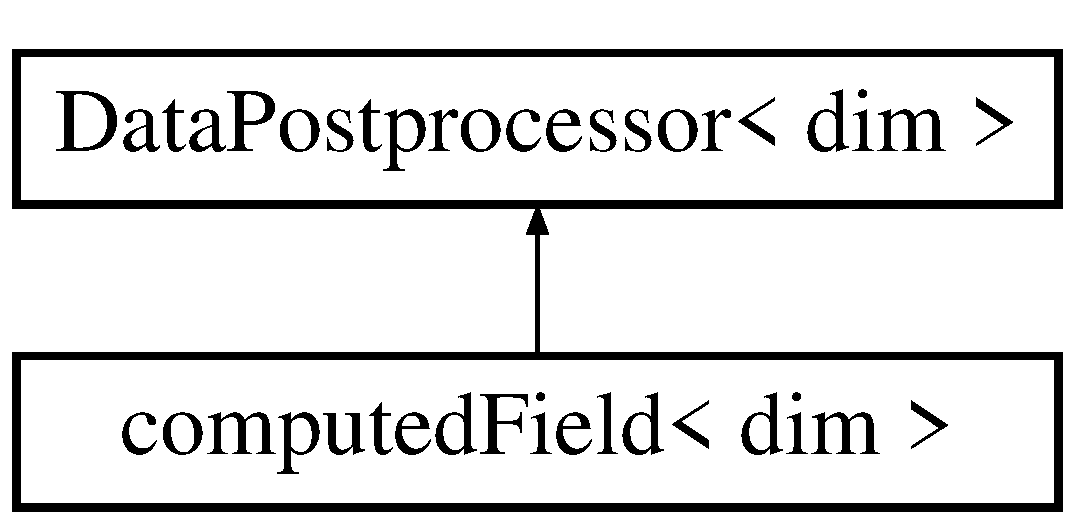
\includegraphics[height=2.000000cm]{classcomputed_field}
\end{center}
\end{figure}
\subsection*{Public Member Functions}
\begin{DoxyCompactItemize}
\item 
\mbox{\hyperlink{classcomputed_field_ab4f4245d1d8abf1daeedbf2784d6c42a}{computed\+Field}} ()
\item 
\mbox{\hyperlink{classcomputed_field_a23cfaecc3df333ef21739f65a72c81ff}{$\sim$computed\+Field}} ()
\item 
void \mbox{\hyperlink{classcomputed_field_ac6ff6cde468abcaa2ee7c9c4fd6b9047}{setup\+Computed\+Field}} (std\+::vector$<$ std\+::vector$<$ std\+::string $>$ $>$ \+\_\+primary\+\_\+variables)
\item 
std\+::vector$<$ std\+::string $>$ \mbox{\hyperlink{classcomputed_field_a08e571d88aae15fdb3162f74bf9fd6e7}{get\+\_\+names}} () const
\item 
std\+::vector$<$ Data\+Component\+Interpretation\+::\+Data\+Component\+Interpretation $>$ \mbox{\hyperlink{classcomputed_field_a3a7ceb57bada784f078912268a0774a7}{get\+\_\+data\+\_\+component\+\_\+interpretation}} () const
\item 
virtual Update\+Flags \mbox{\hyperlink{classcomputed_field_ac3df6aa570f6a91215394fd4951e9f93}{get\+\_\+needed\+\_\+update\+\_\+flags}} () const
\end{DoxyCompactItemize}
\subsection*{Public Attributes}
\begin{DoxyCompactItemize}
\item 
std\+::vector$<$ std\+::vector$<$ std\+::string $>$ $>$ \mbox{\hyperlink{classcomputed_field_a4933860ad833b7b9bd2b8effee5c36d6}{primary\+\_\+variables}}
\end{DoxyCompactItemize}


\subsection{Constructor \& Destructor Documentation}
\mbox{\label{classcomputed_field_ab4f4245d1d8abf1daeedbf2784d6c42a}} 
\index{computedField$<$ dim $>$@{computedField$<$ dim $>$}!computedField@{computedField}}
\index{computedField@{computedField}!computedField$<$ dim $>$@{computedField$<$ dim $>$}}
\subsubsection{\texorpdfstring{computedField()}{computedField()}}
{\footnotesize\ttfamily \mbox{\hyperlink{classcomputed_field}{computed\+Field}} (\begin{DoxyParamCaption}{ }\end{DoxyParamCaption})}

\mbox{\label{classcomputed_field_a23cfaecc3df333ef21739f65a72c81ff}} 
\index{computedField$<$ dim $>$@{computedField$<$ dim $>$}!````~computedField@{$\sim$computedField}}
\index{````~computedField@{$\sim$computedField}!computedField$<$ dim $>$@{computedField$<$ dim $>$}}
\subsubsection{\texorpdfstring{$\sim$computedField()}{~computedField()}}
{\footnotesize\ttfamily $\sim$\mbox{\hyperlink{classcomputed_field}{computed\+Field}} (\begin{DoxyParamCaption}{ }\end{DoxyParamCaption})}



\subsection{Member Function Documentation}
\mbox{\label{classcomputed_field_a3a7ceb57bada784f078912268a0774a7}} 
\index{computedField$<$ dim $>$@{computedField$<$ dim $>$}!get\_data\_component\_interpretation@{get\_data\_component\_interpretation}}
\index{get\_data\_component\_interpretation@{get\_data\_component\_interpretation}!computedField$<$ dim $>$@{computedField$<$ dim $>$}}
\subsubsection{\texorpdfstring{get\_data\_component\_interpretation()}{get\_data\_component\_interpretation()}}
{\footnotesize\ttfamily std\+::vector$<$ Data\+Component\+Interpretation\+::\+Data\+Component\+Interpretation $>$ get\+\_\+data\+\_\+component\+\_\+interpretation (\begin{DoxyParamCaption}{ }\end{DoxyParamCaption}) const}

\mbox{\label{classcomputed_field_a08e571d88aae15fdb3162f74bf9fd6e7}} 
\index{computedField$<$ dim $>$@{computedField$<$ dim $>$}!get\_names@{get\_names}}
\index{get\_names@{get\_names}!computedField$<$ dim $>$@{computedField$<$ dim $>$}}
\subsubsection{\texorpdfstring{get\_names()}{get\_names()}}
{\footnotesize\ttfamily std\+::vector$<$ std\+::string $>$ get\+\_\+names (\begin{DoxyParamCaption}{ }\end{DoxyParamCaption}) const}

\mbox{\label{classcomputed_field_ac3df6aa570f6a91215394fd4951e9f93}} 
\index{computedField$<$ dim $>$@{computedField$<$ dim $>$}!get\_needed\_update\_flags@{get\_needed\_update\_flags}}
\index{get\_needed\_update\_flags@{get\_needed\_update\_flags}!computedField$<$ dim $>$@{computedField$<$ dim $>$}}
\subsubsection{\texorpdfstring{get\_needed\_update\_flags()}{get\_needed\_update\_flags()}}
{\footnotesize\ttfamily Update\+Flags get\+\_\+needed\+\_\+update\+\_\+flags (\begin{DoxyParamCaption}{ }\end{DoxyParamCaption}) const\hspace{0.3cm}{\ttfamily [virtual]}}

\mbox{\label{classcomputed_field_ac6ff6cde468abcaa2ee7c9c4fd6b9047}} 
\index{computedField$<$ dim $>$@{computedField$<$ dim $>$}!setupComputedField@{setupComputedField}}
\index{setupComputedField@{setupComputedField}!computedField$<$ dim $>$@{computedField$<$ dim $>$}}
\subsubsection{\texorpdfstring{setupComputedField()}{setupComputedField()}}
{\footnotesize\ttfamily void setup\+Computed\+Field (\begin{DoxyParamCaption}\item[{std\+::vector$<$ std\+::vector$<$ std\+::string $>$ $>$}]{\+\_\+primary\+\_\+variables }\end{DoxyParamCaption})}

setup names and variable types\+:scalar, vector 

\subsection{Member Data Documentation}
\mbox{\label{classcomputed_field_a4933860ad833b7b9bd2b8effee5c36d6}} 
\index{computedField$<$ dim $>$@{computedField$<$ dim $>$}!primary\_variables@{primary\_variables}}
\index{primary\_variables@{primary\_variables}!computedField$<$ dim $>$@{computedField$<$ dim $>$}}
\subsubsection{\texorpdfstring{primary\_variables}{primary\_variables}}
{\footnotesize\ttfamily std\+::vector$<$std\+::vector$<$std\+::string$>$ $>$ primary\+\_\+variables}



The documentation for this class was generated from the following files\+:\begin{DoxyCompactItemize}
\item 
mechano\+Chem\+F\+E\+M/include/supplementary/\mbox{\hyperlink{computed_field_8h}{computed\+Field.\+h}}\item 
mechano\+Chem\+F\+E\+M/src/supplementary/\mbox{\hyperlink{computed_field_8cc}{computed\+Field.\+cc}}\end{DoxyCompactItemize}

\section{Customer\+Preconditioner$<$ matrix\+Type, vector\+Type $>$ Class Template Reference}
\label{class_customer_preconditioner}\index{CustomerPreconditioner$<$ matrixType, vectorType $>$@{CustomerPreconditioner$<$ matrixType, vectorType $>$}}


{\ttfamily \#include $<$Customer\+Preconditioner.\+h$>$}

Inheritance diagram for Customer\+Preconditioner$<$ matrix\+Type, vector\+Type $>$\+:\begin{figure}[H]
\begin{center}
\leavevmode
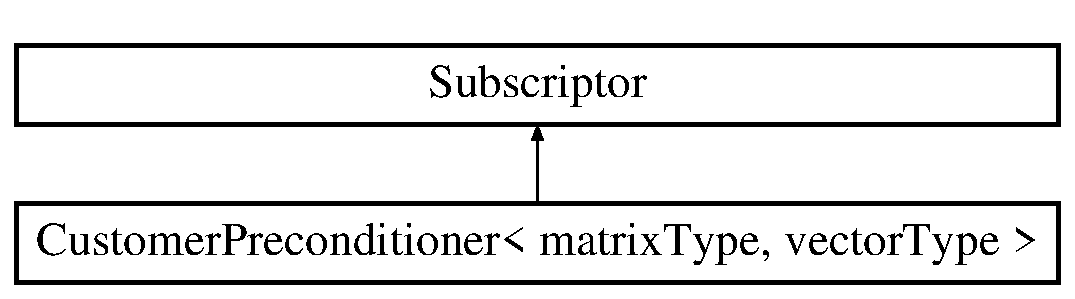
\includegraphics[height=2.000000cm]{class_customer_preconditioner}
\end{center}
\end{figure}
\subsection*{Public Member Functions}
\begin{DoxyCompactItemize}
\item 
\mbox{\hyperlink{class_customer_preconditioner_a3603795be2fcda83add4d39b5905fbcf}{Customer\+Preconditioner}} (const matrix\+Type \&A)
\item 
void \mbox{\hyperlink{class_customer_preconditioner_a1daf83868b73ad6798ea7b70af6a96d8}{vmult}} (vector\+Type \&dst, vector\+Type \&src) const
\end{DoxyCompactItemize}
\subsection*{Private Attributes}
\begin{DoxyCompactItemize}
\item 
const Smart\+Pointer$<$ const matrix\+Type $>$ \mbox{\hyperlink{class_customer_preconditioner_a565a77476d06a1a0c5eaeb48b8fa3736}{system\+\_\+matrix}}
\end{DoxyCompactItemize}


\subsection{Constructor \& Destructor Documentation}
\mbox{\label{class_customer_preconditioner_a3603795be2fcda83add4d39b5905fbcf}} 
\index{CustomerPreconditioner$<$ matrixType, vectorType $>$@{CustomerPreconditioner$<$ matrixType, vectorType $>$}!CustomerPreconditioner@{CustomerPreconditioner}}
\index{CustomerPreconditioner@{CustomerPreconditioner}!CustomerPreconditioner$<$ matrixType, vectorType $>$@{CustomerPreconditioner$<$ matrixType, vectorType $>$}}
\subsubsection{\texorpdfstring{CustomerPreconditioner()}{CustomerPreconditioner()}}
{\footnotesize\ttfamily \mbox{\hyperlink{class_customer_preconditioner}{Customer\+Preconditioner}} (\begin{DoxyParamCaption}\item[{const matrix\+Type \&}]{A }\end{DoxyParamCaption})}



\subsection{Member Function Documentation}
\mbox{\label{class_customer_preconditioner_a1daf83868b73ad6798ea7b70af6a96d8}} 
\index{CustomerPreconditioner$<$ matrixType, vectorType $>$@{CustomerPreconditioner$<$ matrixType, vectorType $>$}!vmult@{vmult}}
\index{vmult@{vmult}!CustomerPreconditioner$<$ matrixType, vectorType $>$@{CustomerPreconditioner$<$ matrixType, vectorType $>$}}
\subsubsection{\texorpdfstring{vmult()}{vmult()}}
{\footnotesize\ttfamily void vmult (\begin{DoxyParamCaption}\item[{vector\+Type \&}]{dst,  }\item[{vector\+Type \&}]{src }\end{DoxyParamCaption}) const}



\subsection{Member Data Documentation}
\mbox{\label{class_customer_preconditioner_a565a77476d06a1a0c5eaeb48b8fa3736}} 
\index{CustomerPreconditioner$<$ matrixType, vectorType $>$@{CustomerPreconditioner$<$ matrixType, vectorType $>$}!system\_matrix@{system\_matrix}}
\index{system\_matrix@{system\_matrix}!CustomerPreconditioner$<$ matrixType, vectorType $>$@{CustomerPreconditioner$<$ matrixType, vectorType $>$}}
\subsubsection{\texorpdfstring{system\_matrix}{system\_matrix}}
{\footnotesize\ttfamily const Smart\+Pointer$<$const matrix\+Type$>$ system\+\_\+matrix\hspace{0.3cm}{\ttfamily [private]}}



The documentation for this class was generated from the following files\+:\begin{DoxyCompactItemize}
\item 
include/supplementary/\mbox{\hyperlink{_customer_preconditioner_8h}{Customer\+Preconditioner.\+h}}\item 
src/supplementary/\mbox{\hyperlink{_customer_preconditioner_8cc}{Customer\+Preconditioner.\+cc}}\end{DoxyCompactItemize}

\section{deformation\+Map$<$ T, dim $>$ Struct Template Reference}
\label{structdeformation_map}\index{deformationMap$<$ T, dim $>$@{deformationMap$<$ T, dim $>$}}


{\ttfamily \#include $<$data\+Struct.\+h$>$}

\subsection*{Public Member Functions}
\begin{DoxyCompactItemize}
\item 
\mbox{\hyperlink{structdeformation_map_a3ce85c3a09b45f207030b97eed6c5e4c}{deformation\+Map}} (unsigned int \+\_\+n\+\_\+q\+\_\+points)
\end{DoxyCompactItemize}
\subsection*{Public Attributes}
\begin{DoxyCompactItemize}
\item 
dealii\+::\+Table$<$ 3, T $>$ \mbox{\hyperlink{structdeformation_map_a7934bed7ba72b5e4a3af1fd8a4e14198}{F}}
\item 
dealii\+::\+Table$<$ 3, T $>$ \mbox{\hyperlink{structdeformation_map_ae40deb9e4616ec6d0b77519e56646ce0}{invF}}
\item 
dealii\+::\+Table$<$ 1, T $>$ \mbox{\hyperlink{structdeformation_map_aa1ff2dc8fb6f4f6e9125ca026505a977}{detF}}
\item 
unsigned int \mbox{\hyperlink{structdeformation_map_a75df8197cf561419d8ead67373abeafd}{n\+\_\+q\+\_\+points}}
\end{DoxyCompactItemize}


\subsection{Constructor \& Destructor Documentation}
\mbox{\label{structdeformation_map_a3ce85c3a09b45f207030b97eed6c5e4c}} 
\index{deformationMap$<$ T, dim $>$@{deformationMap$<$ T, dim $>$}!deformationMap@{deformationMap}}
\index{deformationMap@{deformationMap}!deformationMap$<$ T, dim $>$@{deformationMap$<$ T, dim $>$}}
\subsubsection{\texorpdfstring{deformationMap()}{deformationMap()}}
{\footnotesize\ttfamily \mbox{\hyperlink{structdeformation_map}{deformation\+Map}} (\begin{DoxyParamCaption}\item[{unsigned int}]{\+\_\+n\+\_\+q\+\_\+points }\end{DoxyParamCaption})\hspace{0.3cm}{\ttfamily [inline]}}



\subsection{Member Data Documentation}
\mbox{\label{structdeformation_map_aa1ff2dc8fb6f4f6e9125ca026505a977}} 
\index{deformationMap$<$ T, dim $>$@{deformationMap$<$ T, dim $>$}!detF@{detF}}
\index{detF@{detF}!deformationMap$<$ T, dim $>$@{deformationMap$<$ T, dim $>$}}
\subsubsection{\texorpdfstring{detF}{detF}}
{\footnotesize\ttfamily dealii\+::\+Table$<$1, T$>$ detF}

\mbox{\label{structdeformation_map_a7934bed7ba72b5e4a3af1fd8a4e14198}} 
\index{deformationMap$<$ T, dim $>$@{deformationMap$<$ T, dim $>$}!F@{F}}
\index{F@{F}!deformationMap$<$ T, dim $>$@{deformationMap$<$ T, dim $>$}}
\subsubsection{\texorpdfstring{F}{F}}
{\footnotesize\ttfamily dealii\+::\+Table$<$3, T$>$ F}

\mbox{\label{structdeformation_map_ae40deb9e4616ec6d0b77519e56646ce0}} 
\index{deformationMap$<$ T, dim $>$@{deformationMap$<$ T, dim $>$}!invF@{invF}}
\index{invF@{invF}!deformationMap$<$ T, dim $>$@{deformationMap$<$ T, dim $>$}}
\subsubsection{\texorpdfstring{invF}{invF}}
{\footnotesize\ttfamily dealii\+::\+Table$<$3, T$>$ invF}

\mbox{\label{structdeformation_map_a75df8197cf561419d8ead67373abeafd}} 
\index{deformationMap$<$ T, dim $>$@{deformationMap$<$ T, dim $>$}!n\_q\_points@{n\_q\_points}}
\index{n\_q\_points@{n\_q\_points}!deformationMap$<$ T, dim $>$@{deformationMap$<$ T, dim $>$}}
\subsubsection{\texorpdfstring{n\_q\_points}{n\_q\_points}}
{\footnotesize\ttfamily unsigned int n\+\_\+q\+\_\+points}



The documentation for this struct was generated from the following file\+:\begin{DoxyCompactItemize}
\item 
include/supplementary/\mbox{\hyperlink{data_struct_8h}{data\+Struct.\+h}}\end{DoxyCompactItemize}

\section{deformation\-Mapwith\-Grad$<$ T, dim $>$ Struct Template Reference}
\label{structdeformation_mapwith_grad}\index{deformation\-Mapwith\-Grad$<$ T, dim $>$@{deformation\-Mapwith\-Grad$<$ T, dim $>$}}


{\ttfamily \#include $<$data\-Struct.\-h$>$}

\subsection*{Public Member Functions}
\begin{DoxyCompactItemize}
\item 
\hyperlink{structdeformation_mapwith_grad_a2c6e68ea962afdc7927d312d097d0bd8}{deformation\-Mapwith\-Grad} (unsigned int n\-\_\-q\-\_\-points)
\end{DoxyCompactItemize}
\subsection*{Public Attributes}
\begin{DoxyCompactItemize}
\item 
dealii\-::\-Table$<$ 3, T $>$ \hyperlink{structdeformation_mapwith_grad_a7934bed7ba72b5e4a3af1fd8a4e14198}{F}
\item 
dealii\-::\-Table$<$ 3, T $>$ \hyperlink{structdeformation_mapwith_grad_ae40deb9e4616ec6d0b77519e56646ce0}{inv\-F}
\item 
dealii\-::\-Table$<$ 4, T $>$ \hyperlink{structdeformation_mapwith_grad_a5bd7f05522c7d581d02e4de55682f5f2}{grad\-F}
\item 
dealii\-::\-Table$<$ 1, T $>$ \hyperlink{structdeformation_mapwith_grad_aa1ff2dc8fb6f4f6e9125ca026505a977}{det\-F}
\end{DoxyCompactItemize}


\subsection{Constructor \& Destructor Documentation}
\index{deformation\-Mapwith\-Grad@{deformation\-Mapwith\-Grad}!deformation\-Mapwith\-Grad@{deformation\-Mapwith\-Grad}}
\index{deformation\-Mapwith\-Grad@{deformation\-Mapwith\-Grad}!deformationMapwithGrad@{deformation\-Mapwith\-Grad}}
\subsubsection[{deformation\-Mapwith\-Grad}]{\setlength{\rightskip}{0pt plus 5cm}{\bf deformation\-Mapwith\-Grad} (
\begin{DoxyParamCaption}
\item[{unsigned int}]{n\-\_\-q\-\_\-points}
\end{DoxyParamCaption}
)\hspace{0.3cm}{\ttfamily [inline]}}\label{structdeformation_mapwith_grad_a2c6e68ea962afdc7927d312d097d0bd8}


\subsection{Member Data Documentation}
\index{deformation\-Mapwith\-Grad@{deformation\-Mapwith\-Grad}!det\-F@{det\-F}}
\index{det\-F@{det\-F}!deformationMapwithGrad@{deformation\-Mapwith\-Grad}}
\subsubsection[{det\-F}]{\setlength{\rightskip}{0pt plus 5cm}dealii\-::\-Table$<$1, T$>$ det\-F}\label{structdeformation_mapwith_grad_aa1ff2dc8fb6f4f6e9125ca026505a977}
\index{deformation\-Mapwith\-Grad@{deformation\-Mapwith\-Grad}!F@{F}}
\index{F@{F}!deformationMapwithGrad@{deformation\-Mapwith\-Grad}}
\subsubsection[{F}]{\setlength{\rightskip}{0pt plus 5cm}dealii\-::\-Table$<$3, T$>$ F}\label{structdeformation_mapwith_grad_a7934bed7ba72b5e4a3af1fd8a4e14198}
\index{deformation\-Mapwith\-Grad@{deformation\-Mapwith\-Grad}!grad\-F@{grad\-F}}
\index{grad\-F@{grad\-F}!deformationMapwithGrad@{deformation\-Mapwith\-Grad}}
\subsubsection[{grad\-F}]{\setlength{\rightskip}{0pt plus 5cm}dealii\-::\-Table$<$4, T$>$ grad\-F}\label{structdeformation_mapwith_grad_a5bd7f05522c7d581d02e4de55682f5f2}
\index{deformation\-Mapwith\-Grad@{deformation\-Mapwith\-Grad}!inv\-F@{inv\-F}}
\index{inv\-F@{inv\-F}!deformationMapwithGrad@{deformation\-Mapwith\-Grad}}
\subsubsection[{inv\-F}]{\setlength{\rightskip}{0pt plus 5cm}dealii\-::\-Table$<$3, T$>$ inv\-F}\label{structdeformation_mapwith_grad_ae40deb9e4616ec6d0b77519e56646ce0}


The documentation for this struct was generated from the following file\-:\begin{DoxyCompactItemize}
\item 
mechano\-Chem\-F\-E\-M/include/supplementary/\hyperlink{data_struct_8h}{data\-Struct.\-h}\end{DoxyCompactItemize}

\section{F\-E\-Mdata$<$ dim, vector\-Type $>$ Class Template Reference}
\label{class_f_e_mdata}\index{F\-E\-Mdata$<$ dim, vector\-Type $>$@{F\-E\-Mdata$<$ dim, vector\-Type $>$}}


{\ttfamily \#include $<$F\-E\-Mdata.\-h$>$}

\subsection*{Public Member Functions}
\begin{DoxyCompactItemize}
\item 
\hyperlink{class_f_e_mdata_abb8edbdb28fbec855696a4a02648ad2d}{F\-E\-Mdata} ()
\item 
\hyperlink{class_f_e_mdata_ada690a46b4cec06866ffa32ca2e07c07}{F\-E\-Mdata} (dealii\-::hp\-::\-Do\-F\-Handler$<$ dim $>$ \&\-\_\-dof\-\_\-handler)
\item 
\hyperlink{class_f_e_mdata_ab7baf283d0dd33996919e2530b735d84}{$\sim$\-F\-E\-Mdata} ()
\item 
void \hyperlink{class_f_e_mdata_a770f8539c16d21624bcedc1f6bee9d68}{set\-\_\-output\-\_\-name} (std\-::vector$<$ std\-::vector$<$ std\-::string $>$ $>$ primary\-\_\-variables)
\item 
void \hyperlink{class_f_e_mdata_ac201e22d75178ffe4d4355c53ee0b756}{clear\-\_\-data\-\_\-vectors} ()
\item 
void \hyperlink{class_f_e_mdata_a62d54e01135c4ab0b58f51441732dca3}{write\-\_\-vtk} (vector\-Type \&solution, std\-::string path)
\item 
void \hyperlink{class_f_e_mdata_a1c60b025bc1f1de692cabdd1f253d343}{create\-\_\-vector\-\_\-snapshot} (vector\-Type \&U, std\-::string out\-\_\-snap\-\_\-file, unsigned int precision=16, const bool scientific=true, const bool across=true) const 
\item 
void \hyperlink{class_f_e_mdata_a2611613e158345b619062316e281c4c9}{resume\-\_\-vector\-\_\-from\-\_\-snapshot} (vector\-Type \&Un, std\-::string in\-\_\-snap\-\_\-file)
\end{DoxyCompactItemize}
\subsection*{Public Attributes}
\begin{DoxyCompactItemize}
\item 
dealii\-::hp\-::\-Do\-F\-Handler$<$ dim $>$ $\ast$ \hyperlink{class_f_e_mdata_a38887e3bbeaa16b46355ba99d22e8063}{dof\-\_\-handler}
\item 
dealii\-::\-Data\-Out$<$ dim, \\*
dealii\-::hp\-::\-Do\-F\-Handler$<$ dim $>$ $>$ \hyperlink{class_f_e_mdata_ab8d2ee01f13a0a7b7d2dd50edabbe8b6}{data\-\_\-out}
\item 
std\-::vector$<$ std\-::string $>$ \hyperlink{class_f_e_mdata_a7b00177ad21830fe46a5bf4b1b4a3ea5}{nodal\-\_\-solution\-\_\-names}
\item 
std\-::vector\\*
$<$ dealii\-::\-Data\-Component\-Interpretation\-::\-Data\-Component\-Interpretation $>$ \hyperlink{class_f_e_mdata_a42965751ff10a28b5add7c0bfa265cee}{nodal\-\_\-data\-\_\-component\-\_\-interpretation}
\item 
M\-P\-I\-\_\-\-Comm \hyperlink{class_f_e_mdata_a03728ed636ca889ae407c84d181bc611}{mpi\-\_\-communicator}
\end{DoxyCompactItemize}


\subsection{Constructor \& Destructor Documentation}
\index{F\-E\-Mdata@{F\-E\-Mdata}!F\-E\-Mdata@{F\-E\-Mdata}}
\index{F\-E\-Mdata@{F\-E\-Mdata}!FEMdata@{F\-E\-Mdata}}
\subsubsection[{F\-E\-Mdata}]{\setlength{\rightskip}{0pt plus 5cm}{\bf F\-E\-Mdata} (
\begin{DoxyParamCaption}
{}
\end{DoxyParamCaption}
)}\label{class_f_e_mdata_abb8edbdb28fbec855696a4a02648ad2d}
\index{F\-E\-Mdata@{F\-E\-Mdata}!F\-E\-Mdata@{F\-E\-Mdata}}
\index{F\-E\-Mdata@{F\-E\-Mdata}!FEMdata@{F\-E\-Mdata}}
\subsubsection[{F\-E\-Mdata}]{\setlength{\rightskip}{0pt plus 5cm}{\bf F\-E\-Mdata} (
\begin{DoxyParamCaption}
\item[{dealii\-::hp\-::\-Do\-F\-Handler$<$ dim $>$ \&}]{\-\_\-dof\-\_\-handler}
\end{DoxyParamCaption}
)}\label{class_f_e_mdata_ada690a46b4cec06866ffa32ca2e07c07}
\index{F\-E\-Mdata@{F\-E\-Mdata}!$\sim$\-F\-E\-Mdata@{$\sim$\-F\-E\-Mdata}}
\index{$\sim$\-F\-E\-Mdata@{$\sim$\-F\-E\-Mdata}!FEMdata@{F\-E\-Mdata}}
\subsubsection[{$\sim$\-F\-E\-Mdata}]{\setlength{\rightskip}{0pt plus 5cm}$\sim${\bf F\-E\-Mdata} (
\begin{DoxyParamCaption}
{}
\end{DoxyParamCaption}
)}\label{class_f_e_mdata_ab7baf283d0dd33996919e2530b735d84}


\subsection{Member Function Documentation}
\index{F\-E\-Mdata@{F\-E\-Mdata}!clear\-\_\-data\-\_\-vectors@{clear\-\_\-data\-\_\-vectors}}
\index{clear\-\_\-data\-\_\-vectors@{clear\-\_\-data\-\_\-vectors}!FEMdata@{F\-E\-Mdata}}
\subsubsection[{clear\-\_\-data\-\_\-vectors}]{\setlength{\rightskip}{0pt plus 5cm}void clear\-\_\-data\-\_\-vectors (
\begin{DoxyParamCaption}
{}
\end{DoxyParamCaption}
)}\label{class_f_e_mdata_ac201e22d75178ffe4d4355c53ee0b756}
\index{F\-E\-Mdata@{F\-E\-Mdata}!create\-\_\-vector\-\_\-snapshot@{create\-\_\-vector\-\_\-snapshot}}
\index{create\-\_\-vector\-\_\-snapshot@{create\-\_\-vector\-\_\-snapshot}!FEMdata@{F\-E\-Mdata}}
\subsubsection[{create\-\_\-vector\-\_\-snapshot}]{\setlength{\rightskip}{0pt plus 5cm}void create\-\_\-vector\-\_\-snapshot (
\begin{DoxyParamCaption}
\item[{vector\-Type \&}]{U, }
\item[{std\-::string}]{out\-\_\-snap\-\_\-file, }
\item[{unsigned int}]{precision = {\ttfamily 16}, }
\item[{const bool}]{scientific = {\ttfamily true}, }
\item[{const bool}]{across = {\ttfamily true}}
\end{DoxyParamCaption}
) const}\label{class_f_e_mdata_a1c60b025bc1f1de692cabdd1f253d343}
create snapshot of vector basically do printing of the vector use it with resume\-\_\-vector\-\_\-from\-\_\-snapshot to do restart \index{F\-E\-Mdata@{F\-E\-Mdata}!resume\-\_\-vector\-\_\-from\-\_\-snapshot@{resume\-\_\-vector\-\_\-from\-\_\-snapshot}}
\index{resume\-\_\-vector\-\_\-from\-\_\-snapshot@{resume\-\_\-vector\-\_\-from\-\_\-snapshot}!FEMdata@{F\-E\-Mdata}}
\subsubsection[{resume\-\_\-vector\-\_\-from\-\_\-snapshot}]{\setlength{\rightskip}{0pt plus 5cm}void resume\-\_\-vector\-\_\-from\-\_\-snapshot (
\begin{DoxyParamCaption}
\item[{vector\-Type \&}]{Un, }
\item[{std\-::string}]{in\-\_\-snap\-\_\-file}
\end{DoxyParamCaption}
)}\label{class_f_e_mdata_a2611613e158345b619062316e281c4c9}
resume snapshot of vector stored in 'in\-\_\-snap\-\_\-file' to vector 'Un' according to this dof\-\_\-handler. only works when two vector initialized based on same mesh, otherwise dof sequence and partition would not be recoverd \index{F\-E\-Mdata@{F\-E\-Mdata}!set\-\_\-output\-\_\-name@{set\-\_\-output\-\_\-name}}
\index{set\-\_\-output\-\_\-name@{set\-\_\-output\-\_\-name}!FEMdata@{F\-E\-Mdata}}
\subsubsection[{set\-\_\-output\-\_\-name}]{\setlength{\rightskip}{0pt plus 5cm}void set\-\_\-output\-\_\-name (
\begin{DoxyParamCaption}
\item[{std\-::vector$<$ std\-::vector$<$ std\-::string $>$ $>$}]{primary\-\_\-variables}
\end{DoxyParamCaption}
)}\label{class_f_e_mdata_a770f8539c16d21624bcedc1f6bee9d68}
set nodal\-\_\-solution\-\_\-names and nodal\-\_\-data\-\_\-component\-\_\-interpretation in deal.\-ii convention \index{F\-E\-Mdata@{F\-E\-Mdata}!write\-\_\-vtk@{write\-\_\-vtk}}
\index{write\-\_\-vtk@{write\-\_\-vtk}!FEMdata@{F\-E\-Mdata}}
\subsubsection[{write\-\_\-vtk}]{\setlength{\rightskip}{0pt plus 5cm}void write\-\_\-vtk (
\begin{DoxyParamCaption}
\item[{vector\-Type \&}]{solution, }
\item[{std\-::string}]{path}
\end{DoxyParamCaption}
)}\label{class_f_e_mdata_a62d54e01135c4ab0b58f51441732dca3}
write vtk using solution vector corresponding to this dof\-\_\-handler into path. path is the full directory with file name e.\-g. '/home/output/output.vtk'. 

\subsection{Member Data Documentation}
\index{F\-E\-Mdata@{F\-E\-Mdata}!data\-\_\-out@{data\-\_\-out}}
\index{data\-\_\-out@{data\-\_\-out}!FEMdata@{F\-E\-Mdata}}
\subsubsection[{data\-\_\-out}]{\setlength{\rightskip}{0pt plus 5cm}dealii\-::\-Data\-Out$<$dim,dealii\-::hp\-::\-Do\-F\-Handler$<$dim$>$ $>$ data\-\_\-out}\label{class_f_e_mdata_ab8d2ee01f13a0a7b7d2dd50edabbe8b6}
\index{F\-E\-Mdata@{F\-E\-Mdata}!dof\-\_\-handler@{dof\-\_\-handler}}
\index{dof\-\_\-handler@{dof\-\_\-handler}!FEMdata@{F\-E\-Mdata}}
\subsubsection[{dof\-\_\-handler}]{\setlength{\rightskip}{0pt plus 5cm}dealii\-::hp\-::\-Do\-F\-Handler$<$dim$>$$\ast$ dof\-\_\-handler}\label{class_f_e_mdata_a38887e3bbeaa16b46355ba99d22e8063}
deal.\-ii dof\-\_\-handler \index{F\-E\-Mdata@{F\-E\-Mdata}!mpi\-\_\-communicator@{mpi\-\_\-communicator}}
\index{mpi\-\_\-communicator@{mpi\-\_\-communicator}!FEMdata@{F\-E\-Mdata}}
\subsubsection[{mpi\-\_\-communicator}]{\setlength{\rightskip}{0pt plus 5cm}M\-P\-I\-\_\-\-Comm mpi\-\_\-communicator}\label{class_f_e_mdata_a03728ed636ca889ae407c84d181bc611}
\index{F\-E\-Mdata@{F\-E\-Mdata}!nodal\-\_\-data\-\_\-component\-\_\-interpretation@{nodal\-\_\-data\-\_\-component\-\_\-interpretation}}
\index{nodal\-\_\-data\-\_\-component\-\_\-interpretation@{nodal\-\_\-data\-\_\-component\-\_\-interpretation}!FEMdata@{F\-E\-Mdata}}
\subsubsection[{nodal\-\_\-data\-\_\-component\-\_\-interpretation}]{\setlength{\rightskip}{0pt plus 5cm}std\-::vector$<$dealii\-::\-Data\-Component\-Interpretation\-::\-Data\-Component\-Interpretation$>$ nodal\-\_\-data\-\_\-component\-\_\-interpretation}\label{class_f_e_mdata_a42965751ff10a28b5add7c0bfa265cee}
\index{F\-E\-Mdata@{F\-E\-Mdata}!nodal\-\_\-solution\-\_\-names@{nodal\-\_\-solution\-\_\-names}}
\index{nodal\-\_\-solution\-\_\-names@{nodal\-\_\-solution\-\_\-names}!FEMdata@{F\-E\-Mdata}}
\subsubsection[{nodal\-\_\-solution\-\_\-names}]{\setlength{\rightskip}{0pt plus 5cm}std\-::vector$<$std\-::string$>$ nodal\-\_\-solution\-\_\-names}\label{class_f_e_mdata_a7b00177ad21830fe46a5bf4b1b4a3ea5}


The documentation for this class was generated from the following files\-:\begin{DoxyCompactItemize}
\item 
include/\hyperlink{_f_e_mdata_8h}{F\-E\-Mdata.\-h}\item 
src/\-F\-E\-Mdata/\hyperlink{_f_e_mdata_8cc}{F\-E\-Mdata.\-cc}\item 
src/\-F\-E\-Mdata/\hyperlink{set__output__name_8cc}{set\-\_\-output\-\_\-name.\-cc}\item 
src/\-F\-E\-Mdata/\hyperlink{snapshot_8cc}{snapshot.\-cc}\item 
src/\-F\-E\-Mdata/\hyperlink{write__vtk_8cc}{write\-\_\-vtk.\-cc}\end{DoxyCompactItemize}

\section{hp\-F\-E\-M$<$ dim $>$ Class Template Reference}
\label{classhp_f_e_m}\index{hp\-F\-E\-M$<$ dim $>$@{hp\-F\-E\-M$<$ dim $>$}}


{\ttfamily \#include $<$hp\-F\-E\-M.\-h$>$}

Inheritance diagram for hp\-F\-E\-M$<$ dim $>$\-:\begin{figure}[H]
\begin{center}
\leavevmode
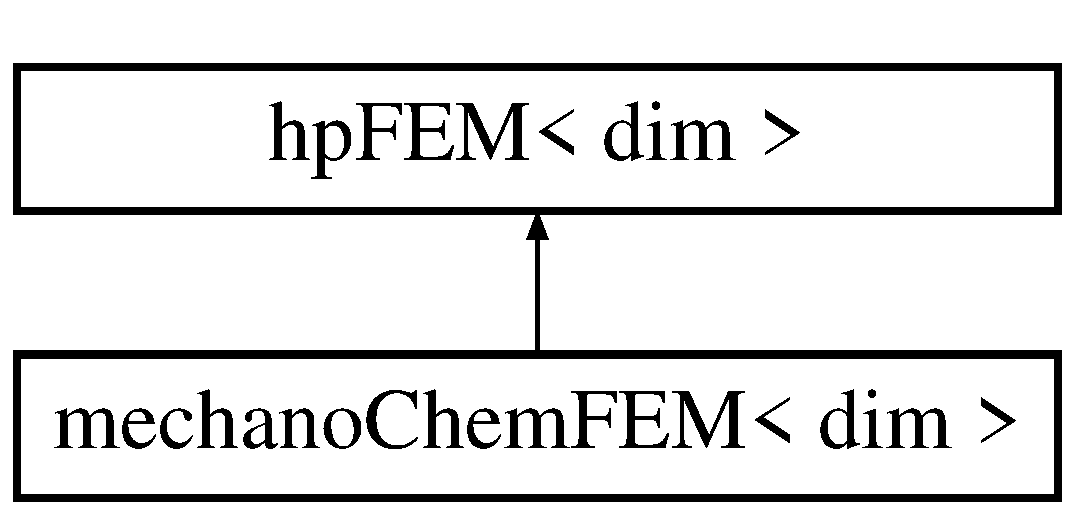
\includegraphics[height=2.000000cm]{classhp_f_e_m}
\end{center}
\end{figure}
\subsection*{Public Member Functions}
\begin{DoxyCompactItemize}
\item 
\hyperlink{classhp_f_e_m_ac1540fdd371c0b89a90809251b618025}{hp\-F\-E\-M} ()
\item 
\hyperlink{classhp_f_e_m_acf426058508649734ee9618b5c9148c1}{$\sim$hp\-F\-E\-M} ()
\item 
void \hyperlink{classhp_f_e_m_afe86b756fb757221f5a8a16c956b7e76}{setup\-\_\-\-Fe\-System} (std\-::vector$<$ std\-::shared\-\_\-ptr$<$ F\-E\-System$<$ dim $>$$>$ $>$ \&fe\-\_\-system, hp\-::\-F\-E\-Collection$<$ dim $>$ \&fe\-\_\-collection, hp\-::\-Q\-Collection$<$ dim $>$ \&q\-\_\-collection, std\-::vector$<$ unsigned int $>$ \&primary\-\_\-variables\-\_\-dof, std\-::vector$<$ std\-::vector$<$ std\-::string $>$ $>$ \&primary\-\_\-variables, std\-::vector$<$ std\-::vector$<$ int $>$ $>$ \&F\-E\-\_\-support, const Q\-Gauss$<$ dim $>$ \&volume\-\_\-quadrature)
\item 
void \hyperlink{classhp_f_e_m_a12205240784051ad249a536cb7ee98d5}{set\-\_\-active\-\_\-fe\-\_\-indices} (std\-::vector$<$ std\-::vector$<$ int $>$ $>$ \&F\-E\-\_\-support, hp\-::\-Do\-F\-Handler$<$ dim $>$ \&local\-\_\-handler, int domain=0)
\item 
int \hyperlink{classhp_f_e_m_a9ceee3881af75e3be863fdb2d1688c0e}{total\-D\-O\-F} (std\-::vector$<$ std\-::vector$<$ std\-::string $>$ $>$ \&primary\-\_\-variables)
\end{DoxyCompactItemize}
\subsection*{Public Attributes}
\begin{DoxyCompactItemize}
\item 
Triangulation$<$ dim $>$ \hyperlink{classhp_f_e_m_a1e604d1e68926caf1ebc67d2a7451783}{triangulation}
\item 
hp\-::\-Do\-F\-Handler$<$ dim $>$ \hyperlink{classhp_f_e_m_ab4df20fb431f370878adc06e19280d62}{dof\-\_\-handler}
\item 
Constraint\-Matrix \hyperlink{classhp_f_e_m_aa08dcec4445eed1687b99cdb7b24b785}{constraints}
\end{DoxyCompactItemize}


\subsection{Detailed Description}
\subsubsection*{template$<$int dim$>$class hp\-F\-E\-M$<$ dim $>$}

This class is intended to be base/abstract class. It contains three essential objects in deal.\-ii\-: {\ttfamily Triangulation$<$dim$>$}, {\ttfamily hp\-::\-Do\-F\-Handler$<$dim$>$} and {\ttfamily Constraint\-Matrix}. Those three will be shared in other classes\-:
\begin{DoxyCode}
solveClass< dim, matrixType, vectorType > and FEMdata< dim, vectorType >
\end{DoxyCode}
 Class hp\-F\-E\-M$<$ dim $>$ also provide functions to 

\subsection{Constructor \& Destructor Documentation}
\index{hp\-F\-E\-M@{hp\-F\-E\-M}!hp\-F\-E\-M@{hp\-F\-E\-M}}
\index{hp\-F\-E\-M@{hp\-F\-E\-M}!hpFEM@{hp\-F\-E\-M}}
\subsubsection[{hp\-F\-E\-M}]{\setlength{\rightskip}{0pt plus 5cm}{\bf hp\-F\-E\-M} (
\begin{DoxyParamCaption}
{}
\end{DoxyParamCaption}
)}\label{classhp_f_e_m_ac1540fdd371c0b89a90809251b618025}
abstract class, do nothing specifically except initializing dof\-\_\-handler with triangulation. \index{hp\-F\-E\-M@{hp\-F\-E\-M}!$\sim$hp\-F\-E\-M@{$\sim$hp\-F\-E\-M}}
\index{$\sim$hp\-F\-E\-M@{$\sim$hp\-F\-E\-M}!hpFEM@{hp\-F\-E\-M}}
\subsubsection[{$\sim$hp\-F\-E\-M}]{\setlength{\rightskip}{0pt plus 5cm}$\sim${\bf hp\-F\-E\-M} (
\begin{DoxyParamCaption}
{}
\end{DoxyParamCaption}
)}\label{classhp_f_e_m_acf426058508649734ee9618b5c9148c1}


\subsection{Member Function Documentation}
\index{hp\-F\-E\-M@{hp\-F\-E\-M}!set\-\_\-active\-\_\-fe\-\_\-indices@{set\-\_\-active\-\_\-fe\-\_\-indices}}
\index{set\-\_\-active\-\_\-fe\-\_\-indices@{set\-\_\-active\-\_\-fe\-\_\-indices}!hpFEM@{hp\-F\-E\-M}}
\subsubsection[{set\-\_\-active\-\_\-fe\-\_\-indices}]{\setlength{\rightskip}{0pt plus 5cm}void set\-\_\-active\-\_\-fe\-\_\-indices (
\begin{DoxyParamCaption}
\item[{std\-::vector$<$ std\-::vector$<$ int $>$ $>$ \&}]{F\-E\-\_\-support, }
\item[{hp\-::\-Do\-F\-Handler$<$ dim $>$ \&}]{local\-\_\-handler, }
\item[{int}]{domain = {\ttfamily 0}}
\end{DoxyParamCaption}
)}\label{classhp_f_e_m_a12205240784051ad249a536cb7ee98d5}
\index{hp\-F\-E\-M@{hp\-F\-E\-M}!setup\-\_\-\-Fe\-System@{setup\-\_\-\-Fe\-System}}
\index{setup\-\_\-\-Fe\-System@{setup\-\_\-\-Fe\-System}!hpFEM@{hp\-F\-E\-M}}
\subsubsection[{setup\-\_\-\-Fe\-System}]{\setlength{\rightskip}{0pt plus 5cm}void setup\-\_\-\-Fe\-System (
\begin{DoxyParamCaption}
\item[{std\-::vector$<$ std\-::shared\-\_\-ptr$<$ F\-E\-System$<$ dim $>$$>$ $>$ \&}]{fe\-\_\-system, }
\item[{hp\-::\-F\-E\-Collection$<$ dim $>$ \&}]{fe\-\_\-collection, }
\item[{hp\-::\-Q\-Collection$<$ dim $>$ \&}]{q\-\_\-collection, }
\item[{std\-::vector$<$ unsigned int $>$ \&}]{primary\-\_\-variables\-\_\-dof, }
\item[{std\-::vector$<$ std\-::vector$<$ std\-::string $>$ $>$ \&}]{primary\-\_\-variables, }
\item[{std\-::vector$<$ std\-::vector$<$ int $>$ $>$ \&}]{F\-E\-\_\-support, }
\item[{const Q\-Gauss$<$ dim $>$ \&}]{volume\-\_\-quadrature}
\end{DoxyParamCaption}
)}\label{classhp_f_e_m_afe86b756fb757221f5a8a16c956b7e76}
\index{hp\-F\-E\-M@{hp\-F\-E\-M}!total\-D\-O\-F@{total\-D\-O\-F}}
\index{total\-D\-O\-F@{total\-D\-O\-F}!hpFEM@{hp\-F\-E\-M}}
\subsubsection[{total\-D\-O\-F}]{\setlength{\rightskip}{0pt plus 5cm}int total\-D\-O\-F (
\begin{DoxyParamCaption}
\item[{std\-::vector$<$ std\-::vector$<$ std\-::string $>$ $>$ \&}]{primary\-\_\-variables}
\end{DoxyParamCaption}
)}\label{classhp_f_e_m_a9ceee3881af75e3be863fdb2d1688c0e}


\subsection{Member Data Documentation}
\index{hp\-F\-E\-M@{hp\-F\-E\-M}!constraints@{constraints}}
\index{constraints@{constraints}!hpFEM@{hp\-F\-E\-M}}
\subsubsection[{constraints}]{\setlength{\rightskip}{0pt plus 5cm}Constraint\-Matrix constraints}\label{classhp_f_e_m_aa08dcec4445eed1687b99cdb7b24b785}
\index{hp\-F\-E\-M@{hp\-F\-E\-M}!dof\-\_\-handler@{dof\-\_\-handler}}
\index{dof\-\_\-handler@{dof\-\_\-handler}!hpFEM@{hp\-F\-E\-M}}
\subsubsection[{dof\-\_\-handler}]{\setlength{\rightskip}{0pt plus 5cm}hp\-::\-Do\-F\-Handler$<$dim$>$ dof\-\_\-handler}\label{classhp_f_e_m_ab4df20fb431f370878adc06e19280d62}
\index{hp\-F\-E\-M@{hp\-F\-E\-M}!triangulation@{triangulation}}
\index{triangulation@{triangulation}!hpFEM@{hp\-F\-E\-M}}
\subsubsection[{triangulation}]{\setlength{\rightskip}{0pt plus 5cm}Triangulation$<$dim$>$ triangulation}\label{classhp_f_e_m_a1e604d1e68926caf1ebc67d2a7451783}


The documentation for this class was generated from the following files\-:\begin{DoxyCompactItemize}
\item 
include/\hyperlink{hp_f_e_m_8h}{hp\-F\-E\-M.\-h}\item 
src/hp\-F\-E\-Mbase/\hyperlink{hp_f_e_m_8cc}{hp\-F\-E\-M.\-cc}\item 
src/hp\-F\-E\-Mbase/\hyperlink{setup___fe_system_8cc}{setup\-\_\-\-Fe\-System.\-cc}\end{DoxyCompactItemize}

\section{init\-Bound\-Val\-Probs$<$ dim $>$ Class Template Reference}
\label{classinit_bound_val_probs}\index{init\-Bound\-Val\-Probs$<$ dim $>$@{init\-Bound\-Val\-Probs$<$ dim $>$}}


{\ttfamily \#include $<$init\-Bound\-Val\-Probs.\-h$>$}

Inheritance diagram for init\-Bound\-Val\-Probs$<$ dim $>$\-:\begin{figure}[H]
\begin{center}
\leavevmode
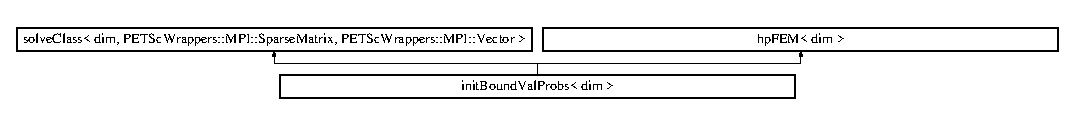
\includegraphics[height=1.100196cm]{classinit_bound_val_probs}
\end{center}
\end{figure}
\subsection*{Public Member Functions}
\begin{DoxyCompactItemize}
\item 
\hyperlink{classinit_bound_val_probs_af836a88e7f9df1d43d6f93c4747858fe}{init\-Bound\-Val\-Probs} (std\-::vector$<$ std\-::vector$<$ std\-::string $>$ $>$ \-\_\-primary\-\_\-variables, std\-::vector$<$ std\-::vector$<$ int $>$ $>$ \-\_\-\-F\-E\-\_\-support, Parameter\-Handler \&\-\_\-params)
\item 
\hyperlink{classinit_bound_val_probs_a38783cfbd559fbad9696ebd823769f53}{$\sim$init\-Bound\-Val\-Probs} ()
\item 
void \hyperlink{classinit_bound_val_probs_af60fa8844da68c0cd887b300855c086c}{declare\-\_\-parameters\-\_\-init\-Bound\-Val\-Probs} ()
\item 
void \hyperlink{classinit_bound_val_probs_a8f0c6272cf214048329d7cf1aa58b860}{setup\-\_\-system} ()
\item 
virtual void \hyperlink{classinit_bound_val_probs_af78c2c6284234c93872188334fb997d8}{update\-Linear\-System} ()
\item 
virtual void \hyperlink{classinit_bound_val_probs_ac8f2c3e2a1040c70b709900dc3dfdaea}{get\-\_\-residual} (const typename hp\-::\-Do\-F\-Handler$<$ dim $>$\-::active\-\_\-cell\-\_\-iterator \&cell, const F\-E\-Values$<$ dim $>$ \&fe\-\_\-values, Table$<$ 1, Sacado\-::\-Fad\-::\-D\-Fad$<$ double $>$ $>$ \&R, Table$<$ 1, Sacado\-::\-Fad\-::\-D\-Fad$<$ double $>$$>$ \&U\-Local, Table$<$ 1, double $>$ \&U\-Local\-Conv)
\item 
virtual void \hyperlink{classinit_bound_val_probs_a7a8df3f99e1d582c6c136b16d6e34d13}{pre\-\_\-run} ()
\item 
virtual void \hyperlink{classinit_bound_val_probs_a13a43e6d814de94978c515cb084873b1}{run} ()
\item 
virtual void \hyperlink{classinit_bound_val_probs_af7d39f0eac0af0ed5785935ac72a1e7d}{solve} ()
\item 
virtual void \hyperlink{classinit_bound_val_probs_aadd4943e52767516f3f7c5460ea35032}{make\-\_\-grid} ()
\item 
virtual void \hyperlink{classinit_bound_val_probs_a7ed791f6f2c777286743182bf2f481bf}{mark\-\_\-boundary} ()
\item 
virtual void \hyperlink{classinit_bound_val_probs_a8d32e81a32f1aaf5682065458548e8e2}{apply\-\_\-initial\-\_\-condition} ()
\item 
virtual void \hyperlink{classinit_bound_val_probs_aea55077652a6fc58f1c0c250c4abd856}{refine\-\_\-grid} ()
\item 
virtual void \hyperlink{classinit_bound_val_probs_a5fb25d0981afa1f7d87875fffcc272c1}{set\-Mult\-Domain} ()
\item 
virtual void \hyperlink{classinit_bound_val_probs_a97967f7bc5aba9a2158464d2de9d2352}{setup\-\_\-constraints} ()
\end{DoxyCompactItemize}
\subsection*{Public Attributes}
\begin{DoxyCompactItemize}
\item 
double \hyperlink{classinit_bound_val_probs_a68c7b36b181a92a91945137308e74a6d}{current\-\_\-dt}
\item 
Parameter\-Handler $\ast$ \hyperlink{classinit_bound_val_probs_a31d5e7a5228d9d55ba00fae854fcfaa0}{params}
\item 
\hyperlink{class_residual}{Residual}$<$ Sacado\-::\-Fad\-::\-D\-Fad\\*
$<$ double $>$, dim $>$ \hyperlink{classinit_bound_val_probs_adeaa7307c79088ccde0e35feb27eb0b0}{Residual\-Eq}
\item 
\hyperlink{class_f_e_mdata}{F\-E\-Mdata}$<$ dim, \\*
P\-E\-T\-Sc\-Wrappers\-::\-M\-P\-I\-::\-Vector $>$ \hyperlink{classinit_bound_val_probs_af7b22336bf40c3a2865dff2cb708136d}{F\-E\-Mdata\-\_\-out}
\item 
std\-::vector$<$ std\-::vector\\*
$<$ std\-::string $>$ $>$ \hyperlink{classinit_bound_val_probs_a4933860ad833b7b9bd2b8effee5c36d6}{primary\-\_\-variables}
\item 
std\-::vector$<$ unsigned int $>$ \hyperlink{classinit_bound_val_probs_a20e37946082ad677ffab164a6dead8b3}{primary\-\_\-variables\-\_\-dof}
\item 
std\-::vector$<$ std\-::vector$<$ int $>$ $>$ \hyperlink{classinit_bound_val_probs_ab0e06106bfe2ab795399d91169290e8a}{F\-E\-\_\-support}
\item 
std\-::vector$<$ std\-::shared\-\_\-ptr\\*
$<$ F\-E\-System$<$ dim $>$ $>$ $>$ \hyperlink{classinit_bound_val_probs_abeb9cdd6078108148320406c68bfa0d1}{fe\-\_\-system}
\item 
P\-E\-T\-Sc\-Wrappers\-::\-M\-P\-I\-::\-Vector \hyperlink{classinit_bound_val_probs_ae539da5c193ce7d8d07f654067f111ca}{solution}
\item 
P\-E\-T\-Sc\-Wrappers\-::\-M\-P\-I\-::\-Vector \hyperlink{classinit_bound_val_probs_ab5b94542feace0c45c2c69696ce9a266}{solution\-\_\-prev}
\item 
const Q\-Gauss$<$ dim $>$ $\ast$ \hyperlink{classinit_bound_val_probs_a7e2363a91f6f1626f463f3a06108c03b}{volume\-\_\-quadrature}
\item 
const Q\-Gauss$<$ dim-\/1 $>$ $\ast$ \hyperlink{classinit_bound_val_probs_af302403bba9078de92d05b4cbe6f44dd}{common\-\_\-face\-\_\-quadrature}
\item 
hp\-::\-F\-E\-Collection$<$ dim $>$ \hyperlink{classinit_bound_val_probs_a02ae472de2833f8763bfe10520be87db}{fe\-\_\-collection}
\item 
hp\-::\-Q\-Collection$<$ dim $>$ \hyperlink{classinit_bound_val_probs_a748ffdb78a6294cd525fe5979bb30649}{q\-\_\-collection}
\item 
Constraint\-Matrix \hyperlink{classinit_bound_val_probs_aa08dcec4445eed1687b99cdb7b24b785}{constraints}
\item 
double \hyperlink{classinit_bound_val_probs_a9db8ce20b0de349987441b8d6830c97a}{domain\-\_\-\-X}
\item 
double \hyperlink{classinit_bound_val_probs_ae7a91557a809cfab5c3dee32ae1de8cb}{domain\-\_\-\-Y}
\item 
double \hyperlink{classinit_bound_val_probs_a199da42cf8a8e51eaeb5cacfdef1c37e}{domain\-\_\-\-Z}
\item 
int \hyperlink{classinit_bound_val_probs_a9a75da991ed1d29646660b1d16a0418f}{current\-\_\-increment}
\item 
double \hyperlink{classinit_bound_val_probs_a557717b333342f1e34a905d6162ce493}{current\-\_\-time}
\item 
double \hyperlink{classinit_bound_val_probs_abc276e47b85df9dd59f248e663b3b971}{total\-\_\-time}
\item 
M\-P\-I\-\_\-\-Comm \hyperlink{classinit_bound_val_probs_a03728ed636ca889ae407c84d181bc611}{mpi\-\_\-communicator}
\item 
const unsigned int \hyperlink{classinit_bound_val_probs_a7320777b83fedaf7a54cdb2fb0ef02e4}{n\-\_\-mpi\-\_\-processes}
\item 
const unsigned int \hyperlink{classinit_bound_val_probs_a6c34addfd3b89faf0a7b4e3fe1236fb0}{this\-\_\-mpi\-\_\-process}
\item 
Conditional\-O\-Stream \hyperlink{classinit_bound_val_probs_a914f651bc9ca2e223b243695dd37ba53}{pcout}
\item 
std\-::string \hyperlink{classinit_bound_val_probs_a95f0e6f488a1faae487cab4198842ebe}{output\-\_\-directory}
\item 
std\-::string \hyperlink{classinit_bound_val_probs_af7ed49a5ea9a6407acb26c5a729d4bd0}{snapshot\-\_\-directory}
\item 
int \hyperlink{classinit_bound_val_probs_a5413329bd1d73152f051cc8d11134f60}{skip\-\_\-output}
\item 
std\-::string \hyperlink{classinit_bound_val_probs_a3ce0cf43eef10e4757e8a225e9b98e96}{snapfile}
\item 
bool \hyperlink{classinit_bound_val_probs_a34ea26077a33f792a9468a4d0ac2feaf}{resuming\-\_\-from\-\_\-snapshot}
\item 
bool \hyperlink{classinit_bound_val_probs_ade455df689de2bc3fb79e1f468fd5404}{save\-\_\-snapshot}
\item 
int \hyperlink{classinit_bound_val_probs_a5b4ed019aaae8f2992f9418a93cd1dbb}{off\-\_\-output\-\_\-index}
\end{DoxyCompactItemize}


\subsection{Constructor \& Destructor Documentation}
\index{init\-Bound\-Val\-Probs@{init\-Bound\-Val\-Probs}!init\-Bound\-Val\-Probs@{init\-Bound\-Val\-Probs}}
\index{init\-Bound\-Val\-Probs@{init\-Bound\-Val\-Probs}!initBoundValProbs@{init\-Bound\-Val\-Probs}}
\subsubsection[{init\-Bound\-Val\-Probs}]{\setlength{\rightskip}{0pt plus 5cm}{\bf init\-Bound\-Val\-Probs} (
\begin{DoxyParamCaption}
\item[{std\-::vector$<$ std\-::vector$<$ std\-::string $>$ $>$}]{\-\_\-primary\-\_\-variables, }
\item[{std\-::vector$<$ std\-::vector$<$ int $>$ $>$}]{\-\_\-\-F\-E\-\_\-support, }
\item[{Parameter\-Handler \&}]{\-\_\-params}
\end{DoxyParamCaption}
)}\label{classinit_bound_val_probs_af836a88e7f9df1d43d6f93c4747858fe}
\index{init\-Bound\-Val\-Probs@{init\-Bound\-Val\-Probs}!$\sim$init\-Bound\-Val\-Probs@{$\sim$init\-Bound\-Val\-Probs}}
\index{$\sim$init\-Bound\-Val\-Probs@{$\sim$init\-Bound\-Val\-Probs}!initBoundValProbs@{init\-Bound\-Val\-Probs}}
\subsubsection[{$\sim$init\-Bound\-Val\-Probs}]{\setlength{\rightskip}{0pt plus 5cm}$\sim${\bf init\-Bound\-Val\-Probs} (
\begin{DoxyParamCaption}
{}
\end{DoxyParamCaption}
)}\label{classinit_bound_val_probs_a38783cfbd559fbad9696ebd823769f53}


\subsection{Member Function Documentation}
\index{init\-Bound\-Val\-Probs@{init\-Bound\-Val\-Probs}!apply\-\_\-initial\-\_\-condition@{apply\-\_\-initial\-\_\-condition}}
\index{apply\-\_\-initial\-\_\-condition@{apply\-\_\-initial\-\_\-condition}!initBoundValProbs@{init\-Bound\-Val\-Probs}}
\subsubsection[{apply\-\_\-initial\-\_\-condition}]{\setlength{\rightskip}{0pt plus 5cm}void apply\-\_\-initial\-\_\-condition (
\begin{DoxyParamCaption}
{}
\end{DoxyParamCaption}
)\hspace{0.3cm}{\ttfamily [virtual]}}\label{classinit_bound_val_probs_a8d32e81a32f1aaf5682065458548e8e2}
default\-: set all solution vector to be zero \index{init\-Bound\-Val\-Probs@{init\-Bound\-Val\-Probs}!declare\-\_\-parameters\-\_\-init\-Bound\-Val\-Probs@{declare\-\_\-parameters\-\_\-init\-Bound\-Val\-Probs}}
\index{declare\-\_\-parameters\-\_\-init\-Bound\-Val\-Probs@{declare\-\_\-parameters\-\_\-init\-Bound\-Val\-Probs}!initBoundValProbs@{init\-Bound\-Val\-Probs}}
\subsubsection[{declare\-\_\-parameters\-\_\-init\-Bound\-Val\-Probs}]{\setlength{\rightskip}{0pt plus 5cm}void declare\-\_\-parameters\-\_\-init\-Bound\-Val\-Probs (
\begin{DoxyParamCaption}
{}
\end{DoxyParamCaption}
)}\label{classinit_bound_val_probs_af60fa8844da68c0cd887b300855c086c}
declare generic paramters \index{init\-Bound\-Val\-Probs@{init\-Bound\-Val\-Probs}!get\-\_\-residual@{get\-\_\-residual}}
\index{get\-\_\-residual@{get\-\_\-residual}!initBoundValProbs@{init\-Bound\-Val\-Probs}}
\subsubsection[{get\-\_\-residual}]{\setlength{\rightskip}{0pt plus 5cm}void get\-\_\-residual (
\begin{DoxyParamCaption}
\item[{const typename hp\-::\-Do\-F\-Handler$<$ dim $>$\-::active\-\_\-cell\-\_\-iterator \&}]{cell, }
\item[{const F\-E\-Values$<$ dim $>$ \&}]{fe\-\_\-values, }
\item[{Table$<$ 1, Sacado\-::\-Fad\-::\-D\-Fad$<$ double $>$ $>$ \&}]{R, }
\item[{Table$<$ 1, Sacado\-::\-Fad\-::\-D\-Fad$<$ double $>$$>$ \&}]{U\-Local, }
\item[{Table$<$ 1, double $>$ \&}]{U\-Local\-Conv}
\end{DoxyParamCaption}
)\hspace{0.3cm}{\ttfamily [virtual]}}\label{classinit_bound_val_probs_ac8f2c3e2a1040c70b709900dc3dfdaea}
abstract function \index{init\-Bound\-Val\-Probs@{init\-Bound\-Val\-Probs}!make\-\_\-grid@{make\-\_\-grid}}
\index{make\-\_\-grid@{make\-\_\-grid}!initBoundValProbs@{init\-Bound\-Val\-Probs}}
\subsubsection[{make\-\_\-grid}]{\setlength{\rightskip}{0pt plus 5cm}void make\-\_\-grid (
\begin{DoxyParamCaption}
{}
\end{DoxyParamCaption}
)\hspace{0.3cm}{\ttfamily [virtual]}}\label{classinit_bound_val_probs_aadd4943e52767516f3f7c5460ea35032}
default\-:make hyper\-\_\-rectangle mesh \index{init\-Bound\-Val\-Probs@{init\-Bound\-Val\-Probs}!mark\-\_\-boundary@{mark\-\_\-boundary}}
\index{mark\-\_\-boundary@{mark\-\_\-boundary}!initBoundValProbs@{init\-Bound\-Val\-Probs}}
\subsubsection[{mark\-\_\-boundary}]{\setlength{\rightskip}{0pt plus 5cm}void mark\-\_\-boundary (
\begin{DoxyParamCaption}
{}
\end{DoxyParamCaption}
)\hspace{0.3cm}{\ttfamily [virtual]}}\label{classinit_bound_val_probs_a7ed791f6f2c777286743182bf2f481bf}
mark boundary \index{init\-Bound\-Val\-Probs@{init\-Bound\-Val\-Probs}!pre\-\_\-run@{pre\-\_\-run}}
\index{pre\-\_\-run@{pre\-\_\-run}!initBoundValProbs@{init\-Bound\-Val\-Probs}}
\subsubsection[{pre\-\_\-run}]{\setlength{\rightskip}{0pt plus 5cm}void pre\-\_\-run (
\begin{DoxyParamCaption}
{}
\end{DoxyParamCaption}
)\hspace{0.3cm}{\ttfamily [virtual]}}\label{classinit_bound_val_probs_a7a8df3f99e1d582c6c136b16d6e34d13}
generic function calls before running the simulations \index{init\-Bound\-Val\-Probs@{init\-Bound\-Val\-Probs}!refine\-\_\-grid@{refine\-\_\-grid}}
\index{refine\-\_\-grid@{refine\-\_\-grid}!initBoundValProbs@{init\-Bound\-Val\-Probs}}
\subsubsection[{refine\-\_\-grid}]{\setlength{\rightskip}{0pt plus 5cm}void refine\-\_\-grid (
\begin{DoxyParamCaption}
{}
\end{DoxyParamCaption}
)\hspace{0.3cm}{\ttfamily [virtual]}}\label{classinit_bound_val_probs_aea55077652a6fc58f1c0c250c4abd856}
default\-: pure virtual function \index{init\-Bound\-Val\-Probs@{init\-Bound\-Val\-Probs}!run@{run}}
\index{run@{run}!initBoundValProbs@{init\-Bound\-Val\-Probs}}
\subsubsection[{run}]{\setlength{\rightskip}{0pt plus 5cm}void run (
\begin{DoxyParamCaption}
{}
\end{DoxyParamCaption}
)\hspace{0.3cm}{\ttfamily [virtual]}}\label{classinit_bound_val_probs_a13a43e6d814de94978c515cb084873b1}
generic function calls to runthe simulations \index{init\-Bound\-Val\-Probs@{init\-Bound\-Val\-Probs}!set\-Mult\-Domain@{set\-Mult\-Domain}}
\index{set\-Mult\-Domain@{set\-Mult\-Domain}!initBoundValProbs@{init\-Bound\-Val\-Probs}}
\subsubsection[{set\-Mult\-Domain}]{\setlength{\rightskip}{0pt plus 5cm}void set\-Mult\-Domain (
\begin{DoxyParamCaption}
{}
\end{DoxyParamCaption}
)\hspace{0.3cm}{\ttfamily [virtual]}}\label{classinit_bound_val_probs_a5fb25d0981afa1f7d87875fffcc272c1}
default\-: pure virtual function \index{init\-Bound\-Val\-Probs@{init\-Bound\-Val\-Probs}!setup\-\_\-constraints@{setup\-\_\-constraints}}
\index{setup\-\_\-constraints@{setup\-\_\-constraints}!initBoundValProbs@{init\-Bound\-Val\-Probs}}
\subsubsection[{setup\-\_\-constraints}]{\setlength{\rightskip}{0pt plus 5cm}void setup\-\_\-constraints (
\begin{DoxyParamCaption}
{}
\end{DoxyParamCaption}
)\hspace{0.3cm}{\ttfamily [virtual]}}\label{classinit_bound_val_probs_a97967f7bc5aba9a2158464d2de9d2352}
default\-: set up constrains \index{init\-Bound\-Val\-Probs@{init\-Bound\-Val\-Probs}!setup\-\_\-system@{setup\-\_\-system}}
\index{setup\-\_\-system@{setup\-\_\-system}!initBoundValProbs@{init\-Bound\-Val\-Probs}}
\subsubsection[{setup\-\_\-system}]{\setlength{\rightskip}{0pt plus 5cm}void setup\-\_\-system (
\begin{DoxyParamCaption}
{}
\end{DoxyParamCaption}
)}\label{classinit_bound_val_probs_a8f0c6272cf214048329d7cf1aa58b860}
this function should not be modified. \index{init\-Bound\-Val\-Probs@{init\-Bound\-Val\-Probs}!solve@{solve}}
\index{solve@{solve}!initBoundValProbs@{init\-Bound\-Val\-Probs}}
\subsubsection[{solve}]{\setlength{\rightskip}{0pt plus 5cm}void solve (
\begin{DoxyParamCaption}
{}
\end{DoxyParamCaption}
)\hspace{0.3cm}{\ttfamily [virtual]}}\label{classinit_bound_val_probs_af7d39f0eac0af0ed5785935ac72a1e7d}
solve \index{init\-Bound\-Val\-Probs@{init\-Bound\-Val\-Probs}!update\-Linear\-System@{update\-Linear\-System}}
\index{update\-Linear\-System@{update\-Linear\-System}!initBoundValProbs@{init\-Bound\-Val\-Probs}}
\subsubsection[{update\-Linear\-System}]{\setlength{\rightskip}{0pt plus 5cm}void update\-Linear\-System (
\begin{DoxyParamCaption}
{}
\end{DoxyParamCaption}
)\hspace{0.3cm}{\ttfamily [virtual]}}\label{classinit_bound_val_probs_af78c2c6284234c93872188334fb997d8}
overload function from solve\-Class 

Reimplemented from \hyperlink{classsolve_class_af78c2c6284234c93872188334fb997d8}{solve\-Class$<$ dim, P\-E\-T\-Sc\-Wrappers\-::\-M\-P\-I\-::\-Sparse\-Matrix, P\-E\-T\-Sc\-Wrappers\-::\-M\-P\-I\-::\-Vector $>$}.



\subsection{Member Data Documentation}
\index{init\-Bound\-Val\-Probs@{init\-Bound\-Val\-Probs}!common\-\_\-face\-\_\-quadrature@{common\-\_\-face\-\_\-quadrature}}
\index{common\-\_\-face\-\_\-quadrature@{common\-\_\-face\-\_\-quadrature}!initBoundValProbs@{init\-Bound\-Val\-Probs}}
\subsubsection[{common\-\_\-face\-\_\-quadrature}]{\setlength{\rightskip}{0pt plus 5cm}const Q\-Gauss$<$dim-\/1$>$$\ast$ common\-\_\-face\-\_\-quadrature}\label{classinit_bound_val_probs_af302403bba9078de92d05b4cbe6f44dd}
\index{init\-Bound\-Val\-Probs@{init\-Bound\-Val\-Probs}!constraints@{constraints}}
\index{constraints@{constraints}!initBoundValProbs@{init\-Bound\-Val\-Probs}}
\subsubsection[{constraints}]{\setlength{\rightskip}{0pt plus 5cm}Constraint\-Matrix constraints}\label{classinit_bound_val_probs_aa08dcec4445eed1687b99cdb7b24b785}
\index{init\-Bound\-Val\-Probs@{init\-Bound\-Val\-Probs}!current\-\_\-dt@{current\-\_\-dt}}
\index{current\-\_\-dt@{current\-\_\-dt}!initBoundValProbs@{init\-Bound\-Val\-Probs}}
\subsubsection[{current\-\_\-dt}]{\setlength{\rightskip}{0pt plus 5cm}double current\-\_\-dt}\label{classinit_bound_val_probs_a68c7b36b181a92a91945137308e74a6d}
\index{init\-Bound\-Val\-Probs@{init\-Bound\-Val\-Probs}!current\-\_\-increment@{current\-\_\-increment}}
\index{current\-\_\-increment@{current\-\_\-increment}!initBoundValProbs@{init\-Bound\-Val\-Probs}}
\subsubsection[{current\-\_\-increment}]{\setlength{\rightskip}{0pt plus 5cm}int current\-\_\-increment}\label{classinit_bound_val_probs_a9a75da991ed1d29646660b1d16a0418f}
\index{init\-Bound\-Val\-Probs@{init\-Bound\-Val\-Probs}!current\-\_\-time@{current\-\_\-time}}
\index{current\-\_\-time@{current\-\_\-time}!initBoundValProbs@{init\-Bound\-Val\-Probs}}
\subsubsection[{current\-\_\-time}]{\setlength{\rightskip}{0pt plus 5cm}double current\-\_\-time}\label{classinit_bound_val_probs_a557717b333342f1e34a905d6162ce493}
\index{init\-Bound\-Val\-Probs@{init\-Bound\-Val\-Probs}!domain\-\_\-\-X@{domain\-\_\-\-X}}
\index{domain\-\_\-\-X@{domain\-\_\-\-X}!initBoundValProbs@{init\-Bound\-Val\-Probs}}
\subsubsection[{domain\-\_\-\-X}]{\setlength{\rightskip}{0pt plus 5cm}double domain\-\_\-\-X}\label{classinit_bound_val_probs_a9db8ce20b0de349987441b8d6830c97a}
\index{init\-Bound\-Val\-Probs@{init\-Bound\-Val\-Probs}!domain\-\_\-\-Y@{domain\-\_\-\-Y}}
\index{domain\-\_\-\-Y@{domain\-\_\-\-Y}!initBoundValProbs@{init\-Bound\-Val\-Probs}}
\subsubsection[{domain\-\_\-\-Y}]{\setlength{\rightskip}{0pt plus 5cm}double domain\-\_\-\-Y}\label{classinit_bound_val_probs_ae7a91557a809cfab5c3dee32ae1de8cb}
\index{init\-Bound\-Val\-Probs@{init\-Bound\-Val\-Probs}!domain\-\_\-\-Z@{domain\-\_\-\-Z}}
\index{domain\-\_\-\-Z@{domain\-\_\-\-Z}!initBoundValProbs@{init\-Bound\-Val\-Probs}}
\subsubsection[{domain\-\_\-\-Z}]{\setlength{\rightskip}{0pt plus 5cm}double domain\-\_\-\-Z}\label{classinit_bound_val_probs_a199da42cf8a8e51eaeb5cacfdef1c37e}
\index{init\-Bound\-Val\-Probs@{init\-Bound\-Val\-Probs}!fe\-\_\-collection@{fe\-\_\-collection}}
\index{fe\-\_\-collection@{fe\-\_\-collection}!initBoundValProbs@{init\-Bound\-Val\-Probs}}
\subsubsection[{fe\-\_\-collection}]{\setlength{\rightskip}{0pt plus 5cm}hp\-::\-F\-E\-Collection$<$dim$>$ fe\-\_\-collection}\label{classinit_bound_val_probs_a02ae472de2833f8763bfe10520be87db}
\index{init\-Bound\-Val\-Probs@{init\-Bound\-Val\-Probs}!F\-E\-\_\-support@{F\-E\-\_\-support}}
\index{F\-E\-\_\-support@{F\-E\-\_\-support}!initBoundValProbs@{init\-Bound\-Val\-Probs}}
\subsubsection[{F\-E\-\_\-support}]{\setlength{\rightskip}{0pt plus 5cm}std\-::vector$<$std\-::vector$<$int$>$ $>$ F\-E\-\_\-support}\label{classinit_bound_val_probs_ab0e06106bfe2ab795399d91169290e8a}
\index{init\-Bound\-Val\-Probs@{init\-Bound\-Val\-Probs}!fe\-\_\-system@{fe\-\_\-system}}
\index{fe\-\_\-system@{fe\-\_\-system}!initBoundValProbs@{init\-Bound\-Val\-Probs}}
\subsubsection[{fe\-\_\-system}]{\setlength{\rightskip}{0pt plus 5cm}std\-::vector$<$std\-::shared\-\_\-ptr$<$F\-E\-System$<$dim$>$ $>$ $>$ fe\-\_\-system}\label{classinit_bound_val_probs_abeb9cdd6078108148320406c68bfa0d1}
\index{init\-Bound\-Val\-Probs@{init\-Bound\-Val\-Probs}!F\-E\-Mdata\-\_\-out@{F\-E\-Mdata\-\_\-out}}
\index{F\-E\-Mdata\-\_\-out@{F\-E\-Mdata\-\_\-out}!initBoundValProbs@{init\-Bound\-Val\-Probs}}
\subsubsection[{F\-E\-Mdata\-\_\-out}]{\setlength{\rightskip}{0pt plus 5cm}{\bf F\-E\-Mdata}$<$dim, P\-E\-T\-Sc\-Wrappers\-::\-M\-P\-I\-::\-Vector$>$ F\-E\-Mdata\-\_\-out}\label{classinit_bound_val_probs_af7b22336bf40c3a2865dff2cb708136d}
\index{init\-Bound\-Val\-Probs@{init\-Bound\-Val\-Probs}!mpi\-\_\-communicator@{mpi\-\_\-communicator}}
\index{mpi\-\_\-communicator@{mpi\-\_\-communicator}!initBoundValProbs@{init\-Bound\-Val\-Probs}}
\subsubsection[{mpi\-\_\-communicator}]{\setlength{\rightskip}{0pt plus 5cm}M\-P\-I\-\_\-\-Comm mpi\-\_\-communicator}\label{classinit_bound_val_probs_a03728ed636ca889ae407c84d181bc611}
\index{init\-Bound\-Val\-Probs@{init\-Bound\-Val\-Probs}!n\-\_\-mpi\-\_\-processes@{n\-\_\-mpi\-\_\-processes}}
\index{n\-\_\-mpi\-\_\-processes@{n\-\_\-mpi\-\_\-processes}!initBoundValProbs@{init\-Bound\-Val\-Probs}}
\subsubsection[{n\-\_\-mpi\-\_\-processes}]{\setlength{\rightskip}{0pt plus 5cm}const unsigned int n\-\_\-mpi\-\_\-processes}\label{classinit_bound_val_probs_a7320777b83fedaf7a54cdb2fb0ef02e4}
\index{init\-Bound\-Val\-Probs@{init\-Bound\-Val\-Probs}!off\-\_\-output\-\_\-index@{off\-\_\-output\-\_\-index}}
\index{off\-\_\-output\-\_\-index@{off\-\_\-output\-\_\-index}!initBoundValProbs@{init\-Bound\-Val\-Probs}}
\subsubsection[{off\-\_\-output\-\_\-index}]{\setlength{\rightskip}{0pt plus 5cm}int off\-\_\-output\-\_\-index}\label{classinit_bound_val_probs_a5b4ed019aaae8f2992f9418a93cd1dbb}
\index{init\-Bound\-Val\-Probs@{init\-Bound\-Val\-Probs}!output\-\_\-directory@{output\-\_\-directory}}
\index{output\-\_\-directory@{output\-\_\-directory}!initBoundValProbs@{init\-Bound\-Val\-Probs}}
\subsubsection[{output\-\_\-directory}]{\setlength{\rightskip}{0pt plus 5cm}std\-::string output\-\_\-directory}\label{classinit_bound_val_probs_a95f0e6f488a1faae487cab4198842ebe}
\index{init\-Bound\-Val\-Probs@{init\-Bound\-Val\-Probs}!params@{params}}
\index{params@{params}!initBoundValProbs@{init\-Bound\-Val\-Probs}}
\subsubsection[{params}]{\setlength{\rightskip}{0pt plus 5cm}Parameter\-Handler$\ast$ params}\label{classinit_bound_val_probs_a31d5e7a5228d9d55ba00fae854fcfaa0}
\index{init\-Bound\-Val\-Probs@{init\-Bound\-Val\-Probs}!pcout@{pcout}}
\index{pcout@{pcout}!initBoundValProbs@{init\-Bound\-Val\-Probs}}
\subsubsection[{pcout}]{\setlength{\rightskip}{0pt plus 5cm}Conditional\-O\-Stream pcout}\label{classinit_bound_val_probs_a914f651bc9ca2e223b243695dd37ba53}
\index{init\-Bound\-Val\-Probs@{init\-Bound\-Val\-Probs}!primary\-\_\-variables@{primary\-\_\-variables}}
\index{primary\-\_\-variables@{primary\-\_\-variables}!initBoundValProbs@{init\-Bound\-Val\-Probs}}
\subsubsection[{primary\-\_\-variables}]{\setlength{\rightskip}{0pt plus 5cm}std\-::vector$<$std\-::vector$<$std\-::string$>$ $>$ primary\-\_\-variables}\label{classinit_bound_val_probs_a4933860ad833b7b9bd2b8effee5c36d6}
\index{init\-Bound\-Val\-Probs@{init\-Bound\-Val\-Probs}!primary\-\_\-variables\-\_\-dof@{primary\-\_\-variables\-\_\-dof}}
\index{primary\-\_\-variables\-\_\-dof@{primary\-\_\-variables\-\_\-dof}!initBoundValProbs@{init\-Bound\-Val\-Probs}}
\subsubsection[{primary\-\_\-variables\-\_\-dof}]{\setlength{\rightskip}{0pt plus 5cm}std\-::vector$<$unsigned int $>$ primary\-\_\-variables\-\_\-dof}\label{classinit_bound_val_probs_a20e37946082ad677ffab164a6dead8b3}
\index{init\-Bound\-Val\-Probs@{init\-Bound\-Val\-Probs}!q\-\_\-collection@{q\-\_\-collection}}
\index{q\-\_\-collection@{q\-\_\-collection}!initBoundValProbs@{init\-Bound\-Val\-Probs}}
\subsubsection[{q\-\_\-collection}]{\setlength{\rightskip}{0pt plus 5cm}hp\-::\-Q\-Collection$<$dim$>$ q\-\_\-collection}\label{classinit_bound_val_probs_a748ffdb78a6294cd525fe5979bb30649}
\index{init\-Bound\-Val\-Probs@{init\-Bound\-Val\-Probs}!Residual\-Eq@{Residual\-Eq}}
\index{Residual\-Eq@{Residual\-Eq}!initBoundValProbs@{init\-Bound\-Val\-Probs}}
\subsubsection[{Residual\-Eq}]{\setlength{\rightskip}{0pt plus 5cm}{\bf Residual}$<$Sacado\-::\-Fad\-::\-D\-Fad$<$double$>$,dim$>$ Residual\-Eq}\label{classinit_bound_val_probs_adeaa7307c79088ccde0e35feb27eb0b0}
\index{init\-Bound\-Val\-Probs@{init\-Bound\-Val\-Probs}!resuming\-\_\-from\-\_\-snapshot@{resuming\-\_\-from\-\_\-snapshot}}
\index{resuming\-\_\-from\-\_\-snapshot@{resuming\-\_\-from\-\_\-snapshot}!initBoundValProbs@{init\-Bound\-Val\-Probs}}
\subsubsection[{resuming\-\_\-from\-\_\-snapshot}]{\setlength{\rightskip}{0pt plus 5cm}bool resuming\-\_\-from\-\_\-snapshot}\label{classinit_bound_val_probs_a34ea26077a33f792a9468a4d0ac2feaf}
\index{init\-Bound\-Val\-Probs@{init\-Bound\-Val\-Probs}!save\-\_\-snapshot@{save\-\_\-snapshot}}
\index{save\-\_\-snapshot@{save\-\_\-snapshot}!initBoundValProbs@{init\-Bound\-Val\-Probs}}
\subsubsection[{save\-\_\-snapshot}]{\setlength{\rightskip}{0pt plus 5cm}bool save\-\_\-snapshot}\label{classinit_bound_val_probs_ade455df689de2bc3fb79e1f468fd5404}
\index{init\-Bound\-Val\-Probs@{init\-Bound\-Val\-Probs}!skip\-\_\-output@{skip\-\_\-output}}
\index{skip\-\_\-output@{skip\-\_\-output}!initBoundValProbs@{init\-Bound\-Val\-Probs}}
\subsubsection[{skip\-\_\-output}]{\setlength{\rightskip}{0pt plus 5cm}int skip\-\_\-output}\label{classinit_bound_val_probs_a5413329bd1d73152f051cc8d11134f60}
\index{init\-Bound\-Val\-Probs@{init\-Bound\-Val\-Probs}!snapfile@{snapfile}}
\index{snapfile@{snapfile}!initBoundValProbs@{init\-Bound\-Val\-Probs}}
\subsubsection[{snapfile}]{\setlength{\rightskip}{0pt plus 5cm}std\-::string snapfile}\label{classinit_bound_val_probs_a3ce0cf43eef10e4757e8a225e9b98e96}
\index{init\-Bound\-Val\-Probs@{init\-Bound\-Val\-Probs}!snapshot\-\_\-directory@{snapshot\-\_\-directory}}
\index{snapshot\-\_\-directory@{snapshot\-\_\-directory}!initBoundValProbs@{init\-Bound\-Val\-Probs}}
\subsubsection[{snapshot\-\_\-directory}]{\setlength{\rightskip}{0pt plus 5cm}std\-::string snapshot\-\_\-directory}\label{classinit_bound_val_probs_af7ed49a5ea9a6407acb26c5a729d4bd0}
\index{init\-Bound\-Val\-Probs@{init\-Bound\-Val\-Probs}!solution@{solution}}
\index{solution@{solution}!initBoundValProbs@{init\-Bound\-Val\-Probs}}
\subsubsection[{solution}]{\setlength{\rightskip}{0pt plus 5cm}P\-E\-T\-Sc\-Wrappers\-::\-M\-P\-I\-::\-Vector solution}\label{classinit_bound_val_probs_ae539da5c193ce7d8d07f654067f111ca}
\index{init\-Bound\-Val\-Probs@{init\-Bound\-Val\-Probs}!solution\-\_\-prev@{solution\-\_\-prev}}
\index{solution\-\_\-prev@{solution\-\_\-prev}!initBoundValProbs@{init\-Bound\-Val\-Probs}}
\subsubsection[{solution\-\_\-prev}]{\setlength{\rightskip}{0pt plus 5cm}P\-E\-T\-Sc\-Wrappers\-::\-M\-P\-I\-::\-Vector solution\-\_\-prev}\label{classinit_bound_val_probs_ab5b94542feace0c45c2c69696ce9a266}
\index{init\-Bound\-Val\-Probs@{init\-Bound\-Val\-Probs}!this\-\_\-mpi\-\_\-process@{this\-\_\-mpi\-\_\-process}}
\index{this\-\_\-mpi\-\_\-process@{this\-\_\-mpi\-\_\-process}!initBoundValProbs@{init\-Bound\-Val\-Probs}}
\subsubsection[{this\-\_\-mpi\-\_\-process}]{\setlength{\rightskip}{0pt plus 5cm}const unsigned int this\-\_\-mpi\-\_\-process}\label{classinit_bound_val_probs_a6c34addfd3b89faf0a7b4e3fe1236fb0}
\index{init\-Bound\-Val\-Probs@{init\-Bound\-Val\-Probs}!total\-\_\-time@{total\-\_\-time}}
\index{total\-\_\-time@{total\-\_\-time}!initBoundValProbs@{init\-Bound\-Val\-Probs}}
\subsubsection[{total\-\_\-time}]{\setlength{\rightskip}{0pt plus 5cm}double total\-\_\-time}\label{classinit_bound_val_probs_abc276e47b85df9dd59f248e663b3b971}
\index{init\-Bound\-Val\-Probs@{init\-Bound\-Val\-Probs}!volume\-\_\-quadrature@{volume\-\_\-quadrature}}
\index{volume\-\_\-quadrature@{volume\-\_\-quadrature}!initBoundValProbs@{init\-Bound\-Val\-Probs}}
\subsubsection[{volume\-\_\-quadrature}]{\setlength{\rightskip}{0pt plus 5cm}const Q\-Gauss$<$dim$>$$\ast$ volume\-\_\-quadrature}\label{classinit_bound_val_probs_a7e2363a91f6f1626f463f3a06108c03b}


The documentation for this class was generated from the following files\-:\begin{DoxyCompactItemize}
\item 
mechano\-Chem\-F\-E\-M/include/\hyperlink{init_bound_val_probs_8h}{init\-Bound\-Val\-Probs.\-h}\item 
mechano\-Chem\-F\-E\-M/src/init\-Bound\-Val\-Probs/\hyperlink{apply__initial__condition_8cc}{apply\-\_\-initial\-\_\-condition.\-cc}\item 
mechano\-Chem\-F\-E\-M/src/init\-Bound\-Val\-Probs/\hyperlink{init_bound_val_probs_2declare__parameters_8cc}{declare\-\_\-parameters.\-cc}\item 
mechano\-Chem\-F\-E\-M/src/init\-Bound\-Val\-Probs/\hyperlink{init_bound_val_probs_8cc}{init\-Bound\-Val\-Probs.\-cc}\item 
mechano\-Chem\-F\-E\-M/src/init\-Bound\-Val\-Probs/\hyperlink{make__grid_8cc}{make\-\_\-grid.\-cc}\item 
mechano\-Chem\-F\-E\-M/src/init\-Bound\-Val\-Probs/\hyperlink{mark__boundary_8cc}{mark\-\_\-boundary.\-cc}\item 
mechano\-Chem\-F\-E\-M/src/init\-Bound\-Val\-Probs/\hyperlink{pre__run_8cc}{pre\-\_\-run.\-cc}\item 
mechano\-Chem\-F\-E\-M/src/init\-Bound\-Val\-Probs/\hyperlink{run_8cc}{run.\-cc}\item 
mechano\-Chem\-F\-E\-M/src/init\-Bound\-Val\-Probs/\hyperlink{setup__constraints_8cc}{setup\-\_\-constraints.\-cc}\item 
mechano\-Chem\-F\-E\-M/src/init\-Bound\-Val\-Probs/\hyperlink{setup__system_8cc}{setup\-\_\-system.\-cc}\item 
mechano\-Chem\-F\-E\-M/src/init\-Bound\-Val\-Probs/\hyperlink{solve_8cc}{solve.\-cc}\item 
mechano\-Chem\-F\-E\-M/src/init\-Bound\-Val\-Probs/\hyperlink{update_linear_system_8cc}{update\-Linear\-System.\-cc}\end{DoxyCompactItemize}

\section{Initial\-Conditions$<$ dim $>$ Class Template Reference}
\label{class_initial_conditions}\index{Initial\-Conditions$<$ dim $>$@{Initial\-Conditions$<$ dim $>$}}


{\ttfamily \#include $<$Initial\-Conditions.\-h$>$}

Inheritance diagram for Initial\-Conditions$<$ dim $>$\-:\begin{figure}[H]
\begin{center}
\leavevmode
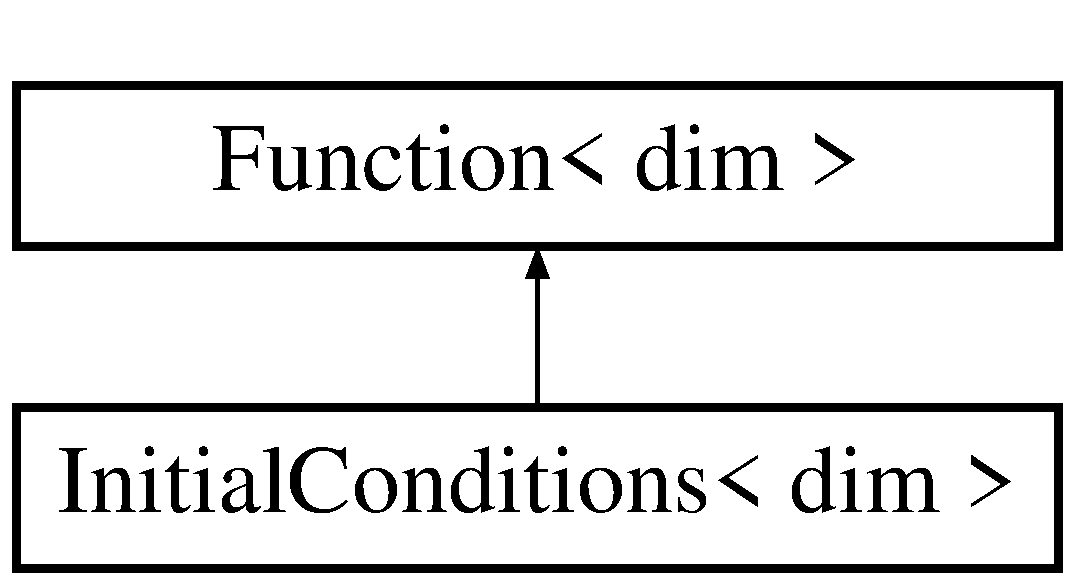
\includegraphics[height=2.000000cm]{class_initial_conditions}
\end{center}
\end{figure}
\subsection*{Public Member Functions}
\begin{DoxyCompactItemize}
\item 
\hyperlink{class_initial_conditions_a86f1233a3d8103059d1a499e1e1d9c04}{Initial\-Conditions} (int \-\_\-total\-D\-O\-F, Parameter\-Handler \&\-\_\-params)
\item 
virtual void \hyperlink{class_initial_conditions_ae2e9e28f0704e62fa54fc7e26dfcd065}{vector\-\_\-value} (const Point$<$ dim $>$ \&p, Vector$<$ double $>$ \&values) const 
\item 
virtual double \hyperlink{class_initial_conditions_af07c55aae0a37d719b86b6471bd9422f}{value} (const Point$<$ dim $>$ \&p, const unsigned int component=0) const 
\end{DoxyCompactItemize}
\subsection*{Public Attributes}
\begin{DoxyCompactItemize}
\item 
int \hyperlink{class_initial_conditions_acf5f14c806d215a0bf5c9f46d3e23607}{total\-D\-O\-F}
\item 
Parameter\-Handler $\ast$ \hyperlink{class_initial_conditions_a31d5e7a5228d9d55ba00fae854fcfaa0}{params}
\end{DoxyCompactItemize}


\subsection{Constructor \& Destructor Documentation}
\index{Initial\-Conditions@{Initial\-Conditions}!Initial\-Conditions@{Initial\-Conditions}}
\index{Initial\-Conditions@{Initial\-Conditions}!InitialConditions@{Initial\-Conditions}}
\subsubsection[{Initial\-Conditions}]{\setlength{\rightskip}{0pt plus 5cm}{\bf Initial\-Conditions} (
\begin{DoxyParamCaption}
\item[{int}]{\-\_\-total\-D\-O\-F, }
\item[{Parameter\-Handler \&}]{\-\_\-params}
\end{DoxyParamCaption}
)}\label{class_initial_conditions_a86f1233a3d8103059d1a499e1e1d9c04}


\subsection{Member Function Documentation}
\index{Initial\-Conditions@{Initial\-Conditions}!value@{value}}
\index{value@{value}!InitialConditions@{Initial\-Conditions}}
\subsubsection[{value}]{\setlength{\rightskip}{0pt plus 5cm}double value (
\begin{DoxyParamCaption}
\item[{const Point$<$ dim $>$ \&}]{p, }
\item[{const unsigned int}]{component = {\ttfamily 0}}
\end{DoxyParamCaption}
) const\hspace{0.3cm}{\ttfamily [virtual]}}\label{class_initial_conditions_af07c55aae0a37d719b86b6471bd9422f}
\index{Initial\-Conditions@{Initial\-Conditions}!vector\-\_\-value@{vector\-\_\-value}}
\index{vector\-\_\-value@{vector\-\_\-value}!InitialConditions@{Initial\-Conditions}}
\subsubsection[{vector\-\_\-value}]{\setlength{\rightskip}{0pt plus 5cm}void vector\-\_\-value (
\begin{DoxyParamCaption}
\item[{const Point$<$ dim $>$ \&}]{p, }
\item[{Vector$<$ double $>$ \&}]{values}
\end{DoxyParamCaption}
) const\hspace{0.3cm}{\ttfamily [virtual]}}\label{class_initial_conditions_ae2e9e28f0704e62fa54fc7e26dfcd065}


\subsection{Member Data Documentation}
\index{Initial\-Conditions@{Initial\-Conditions}!params@{params}}
\index{params@{params}!InitialConditions@{Initial\-Conditions}}
\subsubsection[{params}]{\setlength{\rightskip}{0pt plus 5cm}Parameter\-Handler$\ast$ params}\label{class_initial_conditions_a31d5e7a5228d9d55ba00fae854fcfaa0}
\index{Initial\-Conditions@{Initial\-Conditions}!total\-D\-O\-F@{total\-D\-O\-F}}
\index{total\-D\-O\-F@{total\-D\-O\-F}!InitialConditions@{Initial\-Conditions}}
\subsubsection[{total\-D\-O\-F}]{\setlength{\rightskip}{0pt plus 5cm}int total\-D\-O\-F}\label{class_initial_conditions_acf5f14c806d215a0bf5c9f46d3e23607}


The documentation for this class was generated from the following files\-:\begin{DoxyCompactItemize}
\item 
include/supplementary/\hyperlink{_initial_conditions_8h}{Initial\-Conditions.\-h}\item 
src/supplementary/\hyperlink{_initial_conditions_8cc}{Initial\-Conditions.\-cc}\end{DoxyCompactItemize}

\section{parameters\+Class$<$ dim $>$ Class Template Reference}
\label{classparameters_class}\index{parameters\+Class$<$ dim $>$@{parameters\+Class$<$ dim $>$}}


{\ttfamily \#include $<$parameters.\+h$>$}

\subsection*{Public Member Functions}
\begin{DoxyCompactItemize}
\item 
void \mbox{\hyperlink{classparameters_class_ab2755d1057bef657585eb7fdb7d4b5c4}{set\+Double}} (std\+::string param, double value, bool print=false)
\item 
void \mbox{\hyperlink{classparameters_class_a68203d58af0caf8d232ca9a6fcb0a190}{set\+Int}} (std\+::string param, int value, bool print=false)
\item 
void \mbox{\hyperlink{classparameters_class_a8250a061bef7ccda26e06678c8935f43}{set\+Unsigned\+Int}} (std\+::string param, unsigned int value, bool print=false)
\item 
void \mbox{\hyperlink{classparameters_class_a182ca3f26a78847edd31e99fe68059da}{set\+Bool}} (std\+::string param, bool value, bool print=false)
\item 
void \mbox{\hyperlink{classparameters_class_ab06f012067df1884ecc3a71488aa9ca3}{set\+String}} (std\+::string param, std\+::string value, bool print=false)
\item 
void \mbox{\hyperlink{classparameters_class_aeb69e592e5c35d16379edd69a45af4fd}{set\+Point}} (std\+::string param, double value\mbox{[}dim\mbox{]}, bool print=false)
\item 
double \mbox{\hyperlink{classparameters_class_a40b9baa33a85fa60f5df2996d7dec98b}{get\+Double}} (std\+::string param)
\item 
int \mbox{\hyperlink{classparameters_class_aa97dc7db4ec450afd1cb8bd0d8e00d12}{get\+Int}} (std\+::string param)
\item 
unsigned int \mbox{\hyperlink{classparameters_class_ac01aa6fa0c3b6914b0e7b75128c99bc3}{get\+Unsigned\+Int}} (std\+::string param)
\item 
bool \mbox{\hyperlink{classparameters_class_a7c4393bb42319d396ddf38c2464c7062}{get\+Bool}} (std\+::string param)
\item 
std\+::string \mbox{\hyperlink{classparameters_class_a988c0deb4c2cf7e8ed80e39498c1eb58}{get\+String}} (std\+::string param)
\item 
dealii\+::\+Point$<$ dim $>$ \mbox{\hyperlink{classparameters_class_ab98c50b2209c80346a3e6efdd71589b5}{get\+Point}} (std\+::string param)
\end{DoxyCompactItemize}
\subsection*{Private Attributes}
\begin{DoxyCompactItemize}
\item 
std\+::map$<$ std\+::string, int $>$ \mbox{\hyperlink{classparameters_class_ac8ac4bc08d6cb6aed011bb1d0fc1203f}{p\+Int}}
\item 
std\+::map$<$ std\+::string, unsigned int $>$ \mbox{\hyperlink{classparameters_class_a997bcb31fee3242f776c7e05d709ce12}{p\+Unsigned\+Int}}
\item 
std\+::map$<$ std\+::string, double $>$ \mbox{\hyperlink{classparameters_class_a1e0e610c04bda534bcd48bb81ad75ffc}{p\+Double}}
\item 
std\+::map$<$ std\+::string, bool $>$ \mbox{\hyperlink{classparameters_class_abb7d3139bc101537c7f85fedfe94da2f}{p\+Bool}}
\item 
std\+::map$<$ std\+::string, std\+::string $>$ \mbox{\hyperlink{classparameters_class_a3453601308e73bcc0f45ed6ea8a9959b}{p\+String}}
\item 
std\+::map$<$ std\+::string, dealii\+::\+Point$<$ dim $>$ $>$ \mbox{\hyperlink{classparameters_class_a619a83b172e412339a12ea402580662c}{p\+Point}}
\end{DoxyCompactItemize}


\subsection{Detailed Description}
\subsubsection*{template$<$int dim$>$\newline
class parameters\+Class$<$ dim $>$}

Provide parameters storage, 

\subsection{Member Function Documentation}
\mbox{\label{classparameters_class_a7c4393bb42319d396ddf38c2464c7062}} 
\index{parameters\+Class@{parameters\+Class}!get\+Bool@{get\+Bool}}
\index{get\+Bool@{get\+Bool}!parameters\+Class@{parameters\+Class}}
\subsubsection{\texorpdfstring{get\+Bool()}{getBool()}}
{\footnotesize\ttfamily bool get\+Bool (\begin{DoxyParamCaption}\item[{std\+::string}]{param }\end{DoxyParamCaption})}

\mbox{\label{classparameters_class_a40b9baa33a85fa60f5df2996d7dec98b}} 
\index{parameters\+Class@{parameters\+Class}!get\+Double@{get\+Double}}
\index{get\+Double@{get\+Double}!parameters\+Class@{parameters\+Class}}
\subsubsection{\texorpdfstring{get\+Double()}{getDouble()}}
{\footnotesize\ttfamily double get\+Double (\begin{DoxyParamCaption}\item[{std\+::string}]{param }\end{DoxyParamCaption})}

\mbox{\label{classparameters_class_aa97dc7db4ec450afd1cb8bd0d8e00d12}} 
\index{parameters\+Class@{parameters\+Class}!get\+Int@{get\+Int}}
\index{get\+Int@{get\+Int}!parameters\+Class@{parameters\+Class}}
\subsubsection{\texorpdfstring{get\+Int()}{getInt()}}
{\footnotesize\ttfamily int get\+Int (\begin{DoxyParamCaption}\item[{std\+::string}]{param }\end{DoxyParamCaption})}

\mbox{\label{classparameters_class_ab98c50b2209c80346a3e6efdd71589b5}} 
\index{parameters\+Class@{parameters\+Class}!get\+Point@{get\+Point}}
\index{get\+Point@{get\+Point}!parameters\+Class@{parameters\+Class}}
\subsubsection{\texorpdfstring{get\+Point()}{getPoint()}}
{\footnotesize\ttfamily dealii\+::\+Point$<$ dim $>$ get\+Point (\begin{DoxyParamCaption}\item[{std\+::string}]{param }\end{DoxyParamCaption})}

\mbox{\label{classparameters_class_a988c0deb4c2cf7e8ed80e39498c1eb58}} 
\index{parameters\+Class@{parameters\+Class}!get\+String@{get\+String}}
\index{get\+String@{get\+String}!parameters\+Class@{parameters\+Class}}
\subsubsection{\texorpdfstring{get\+String()}{getString()}}
{\footnotesize\ttfamily std\+::string get\+String (\begin{DoxyParamCaption}\item[{std\+::string}]{param }\end{DoxyParamCaption})}

\mbox{\label{classparameters_class_ac01aa6fa0c3b6914b0e7b75128c99bc3}} 
\index{parameters\+Class@{parameters\+Class}!get\+Unsigned\+Int@{get\+Unsigned\+Int}}
\index{get\+Unsigned\+Int@{get\+Unsigned\+Int}!parameters\+Class@{parameters\+Class}}
\subsubsection{\texorpdfstring{get\+Unsigned\+Int()}{getUnsignedInt()}}
{\footnotesize\ttfamily unsigned int get\+Unsigned\+Int (\begin{DoxyParamCaption}\item[{std\+::string}]{param }\end{DoxyParamCaption})}

\mbox{\label{classparameters_class_a182ca3f26a78847edd31e99fe68059da}} 
\index{parameters\+Class@{parameters\+Class}!set\+Bool@{set\+Bool}}
\index{set\+Bool@{set\+Bool}!parameters\+Class@{parameters\+Class}}
\subsubsection{\texorpdfstring{set\+Bool()}{setBool()}}
{\footnotesize\ttfamily void set\+Bool (\begin{DoxyParamCaption}\item[{std\+::string}]{param,  }\item[{bool}]{value,  }\item[{bool}]{print = {\ttfamily false} }\end{DoxyParamCaption})}

\mbox{\label{classparameters_class_ab2755d1057bef657585eb7fdb7d4b5c4}} 
\index{parameters\+Class@{parameters\+Class}!set\+Double@{set\+Double}}
\index{set\+Double@{set\+Double}!parameters\+Class@{parameters\+Class}}
\subsubsection{\texorpdfstring{set\+Double()}{setDouble()}}
{\footnotesize\ttfamily void set\+Double (\begin{DoxyParamCaption}\item[{std\+::string}]{param,  }\item[{double}]{value,  }\item[{bool}]{print = {\ttfamily false} }\end{DoxyParamCaption})}

\mbox{\label{classparameters_class_a68203d58af0caf8d232ca9a6fcb0a190}} 
\index{parameters\+Class@{parameters\+Class}!set\+Int@{set\+Int}}
\index{set\+Int@{set\+Int}!parameters\+Class@{parameters\+Class}}
\subsubsection{\texorpdfstring{set\+Int()}{setInt()}}
{\footnotesize\ttfamily void set\+Int (\begin{DoxyParamCaption}\item[{std\+::string}]{param,  }\item[{int}]{value,  }\item[{bool}]{print = {\ttfamily false} }\end{DoxyParamCaption})}

\mbox{\label{classparameters_class_aeb69e592e5c35d16379edd69a45af4fd}} 
\index{parameters\+Class@{parameters\+Class}!set\+Point@{set\+Point}}
\index{set\+Point@{set\+Point}!parameters\+Class@{parameters\+Class}}
\subsubsection{\texorpdfstring{set\+Point()}{setPoint()}}
{\footnotesize\ttfamily void set\+Point (\begin{DoxyParamCaption}\item[{std\+::string}]{param,  }\item[{double}]{value\mbox{[}dim\mbox{]},  }\item[{bool}]{print = {\ttfamily false} }\end{DoxyParamCaption})}

\mbox{\label{classparameters_class_ab06f012067df1884ecc3a71488aa9ca3}} 
\index{parameters\+Class@{parameters\+Class}!set\+String@{set\+String}}
\index{set\+String@{set\+String}!parameters\+Class@{parameters\+Class}}
\subsubsection{\texorpdfstring{set\+String()}{setString()}}
{\footnotesize\ttfamily void set\+String (\begin{DoxyParamCaption}\item[{std\+::string}]{param,  }\item[{std\+::string}]{value,  }\item[{bool}]{print = {\ttfamily false} }\end{DoxyParamCaption})}

\mbox{\label{classparameters_class_a8250a061bef7ccda26e06678c8935f43}} 
\index{parameters\+Class@{parameters\+Class}!set\+Unsigned\+Int@{set\+Unsigned\+Int}}
\index{set\+Unsigned\+Int@{set\+Unsigned\+Int}!parameters\+Class@{parameters\+Class}}
\subsubsection{\texorpdfstring{set\+Unsigned\+Int()}{setUnsignedInt()}}
{\footnotesize\ttfamily void set\+Unsigned\+Int (\begin{DoxyParamCaption}\item[{std\+::string}]{param,  }\item[{unsigned int}]{value,  }\item[{bool}]{print = {\ttfamily false} }\end{DoxyParamCaption})}



\subsection{Member Data Documentation}
\mbox{\label{classparameters_class_abb7d3139bc101537c7f85fedfe94da2f}} 
\index{parameters\+Class@{parameters\+Class}!p\+Bool@{p\+Bool}}
\index{p\+Bool@{p\+Bool}!parameters\+Class@{parameters\+Class}}
\subsubsection{\texorpdfstring{p\+Bool}{pBool}}
{\footnotesize\ttfamily std\+::map$<$std\+::string, bool$>$ p\+Bool\hspace{0.3cm}{\ttfamily [private]}}

\mbox{\label{classparameters_class_a1e0e610c04bda534bcd48bb81ad75ffc}} 
\index{parameters\+Class@{parameters\+Class}!p\+Double@{p\+Double}}
\index{p\+Double@{p\+Double}!parameters\+Class@{parameters\+Class}}
\subsubsection{\texorpdfstring{p\+Double}{pDouble}}
{\footnotesize\ttfamily std\+::map$<$std\+::string, double$>$ p\+Double\hspace{0.3cm}{\ttfamily [private]}}

\mbox{\label{classparameters_class_ac8ac4bc08d6cb6aed011bb1d0fc1203f}} 
\index{parameters\+Class@{parameters\+Class}!p\+Int@{p\+Int}}
\index{p\+Int@{p\+Int}!parameters\+Class@{parameters\+Class}}
\subsubsection{\texorpdfstring{p\+Int}{pInt}}
{\footnotesize\ttfamily std\+::map$<$std\+::string, int$>$ p\+Int\hspace{0.3cm}{\ttfamily [private]}}

\mbox{\label{classparameters_class_a619a83b172e412339a12ea402580662c}} 
\index{parameters\+Class@{parameters\+Class}!p\+Point@{p\+Point}}
\index{p\+Point@{p\+Point}!parameters\+Class@{parameters\+Class}}
\subsubsection{\texorpdfstring{p\+Point}{pPoint}}
{\footnotesize\ttfamily std\+::map$<$std\+::string, dealii\+::\+Point$<$dim$>$ $>$ p\+Point\hspace{0.3cm}{\ttfamily [private]}}

\mbox{\label{classparameters_class_a3453601308e73bcc0f45ed6ea8a9959b}} 
\index{parameters\+Class@{parameters\+Class}!p\+String@{p\+String}}
\index{p\+String@{p\+String}!parameters\+Class@{parameters\+Class}}
\subsubsection{\texorpdfstring{p\+String}{pString}}
{\footnotesize\ttfamily std\+::map$<$std\+::string, std\+::string$>$ p\+String\hspace{0.3cm}{\ttfamily [private]}}

\mbox{\label{classparameters_class_a997bcb31fee3242f776c7e05d709ce12}} 
\index{parameters\+Class@{parameters\+Class}!p\+Unsigned\+Int@{p\+Unsigned\+Int}}
\index{p\+Unsigned\+Int@{p\+Unsigned\+Int}!parameters\+Class@{parameters\+Class}}
\subsubsection{\texorpdfstring{p\+Unsigned\+Int}{pUnsignedInt}}
{\footnotesize\ttfamily std\+::map$<$std\+::string, unsigned int$>$ p\+Unsigned\+Int\hspace{0.3cm}{\ttfamily [private]}}



The documentation for this class was generated from the following files\+:\begin{DoxyCompactItemize}
\item 
include/supplementary/\mbox{\hyperlink{parameters_8h}{parameters.\+h}}\item 
src/supplementary/\mbox{\hyperlink{parameters_8cc}{parameters.\+cc}}\end{DoxyCompactItemize}

\section{Residual$<$ T, dim $>$ Class Template Reference}
\label{class_residual}\index{Residual$<$ T, dim $>$@{Residual$<$ T, dim $>$}}


{\ttfamily \#include $<$Residual.\+h$>$}

\subsection*{Public Member Functions}
\begin{DoxyCompactItemize}
\item 
\mbox{\hyperlink{class_residual_a4b540ba8e3ad0a1f8cfe2b4acd20493b}{Residual}} ()
\item 
\mbox{\hyperlink{class_residual_a8eef8c757003dd763b7dddc733f65641}{$\sim$\+Residual}} ()
\item 
void \mbox{\hyperlink{class_residual_a74a86942f009e483e946ac0a0036bd71}{set\+Lame\+Parameters\+By\+Youngs\+Modulus\+Poisson\+Ratio}} (double youngs\+Modulus, double poisson\+Ratio)
\item 
double \mbox{\hyperlink{class_residual_a10e7144d5c4746f15a48d506830790cb}{S\+V\+K3D}} (unsigned int i, unsigned int j, unsigned int k, unsigned int l)
\item 
double \mbox{\hyperlink{class_residual_abd1627afa72ac735e6907067e1d47bb6}{S\+V\+K2D}} (unsigned int i, unsigned int j)
\item 
void \mbox{\hyperlink{class_residual_a4b181b84ebad5e2adb629b4a542dc9c6}{evaluate\+Strain}} (dealii\+::\+Table$<$ 3, T $>$ \&Fe, dealii\+::\+Table$<$ 3, T $>$ \&E, \mbox{\hyperlink{structdeformation_map}{deformation\+Map}}$<$ T, dim $>$ \&def\+Map, bool infinitesimal\+\_\+strain\+\_\+indicator=false)
\item 
void \mbox{\hyperlink{class_residual_a4215ec5a6eabd7573e0caeee6fd194ad}{evaluate\+Saint\+\_\+\+Venant\+\_\+\+Kirchhoff\+Stress}} (dealii\+::\+Table$<$ 3, T $>$ \&P, dealii\+::\+Table$<$ 3, T $>$ \&Fe, dealii\+::\+Table$<$ 3, T $>$ \&E)
\item 
void \mbox{\hyperlink{class_residual_a0f9ff6a237d377803ce368b26ca39652}{evaluate\+Neo\+Hookean\+Stress}} (dealii\+::\+Table$<$ 3, T $>$ \&P, dealii\+::\+Table$<$ 3, T $>$ \&Fe)
\item 
void \mbox{\hyperlink{class_residual_a432fe02216f182fd241f09775131f854}{residual\+For\+Mechanics}} (const F\+E\+Values$<$ dim $>$ \&fe\+\_\+values, unsigned int D\+OF, Table$<$ 1, T $>$ \&R, dealii\+::\+Table$<$ 3, T $>$ P)
\item 
void \mbox{\hyperlink{class_residual_a4c8fd158c8034b25780abfe785755baa}{residual\+For\+Neumman\+BC}} (const F\+E\+Values$<$ dim $>$ \&fe\+\_\+values, const F\+E\+Face\+Values$<$ dim $>$ \&fe\+\_\+face\+\_\+values, unsigned int D\+OF, dealii\+::\+Table$<$ 1, T $>$ \&R, dealii\+::\+Table$<$ 2, T $>$ \&gradn)
\item 
void \mbox{\hyperlink{class_residual_a9a8f493fb66e0bd394948af13a27d821}{residual\+For\+Stokes\+Eq}} (const F\+E\+Values$<$ dim $>$ \&fe\+\_\+values, unsigned int D\+OF, Table$<$ 1, T $>$ \&R, Table$<$ 3, T $>$ \&gradV, dealii\+::\+Table$<$ 1, T $>$ \&pressure)
\item 
void \mbox{\hyperlink{class_residual_a95ad863ab9066d2dbfef9db3907a911f}{residual\+For\+Stokes\+Eq}} (const F\+E\+Values$<$ dim $>$ \&fe\+\_\+values, unsigned int D\+OF, Table$<$ 1, T $>$ \&R, \mbox{\hyperlink{structdeformation_map}{deformation\+Map}}$<$ T, dim $>$ \&def\+Map, Table$<$ 3, T $>$ \&gradV, dealii\+::\+Table$<$ 1, T $>$ \&pressure)
\item 
void \mbox{\hyperlink{class_residual_a34f1f680e957e21ac47c35f404e9fd6a}{residual\+For\+Navier\+\_\+\+Stokes\+Eq}} (const F\+E\+Values$<$ dim $>$ \&fe\+\_\+values, unsigned int D\+OF, Table$<$ 1, T $>$ \&R, \mbox{\hyperlink{structdeformation_map}{deformation\+Map}}$<$ T, dim $>$ \&def\+Map, Table$<$ 2, T $>$ \&V, dealii\+::\+Table$<$ 2, double $>$ \&V\+\_\+conv, Table$<$ 3, T $>$ \&gradV, dealii\+::\+Table$<$ 1, T $>$ \&pressure)
\item 
void \mbox{\hyperlink{class_residual_a7e33928364e99df9a42db58752aca7f3}{evaluate\+Stokes\+Stress}} (dealii\+::\+Table$<$ 3, T $>$ P\+\_\+stoke, const F\+E\+Values$<$ dim $>$ \&fe\+\_\+values, Table$<$ 3, T $>$ \&gradV, dealii\+::\+Table$<$ 1, T $>$ \&pressure)
\item 
void \mbox{\hyperlink{class_residual_a882f4595a6547599cfe8f65897f45896}{residual\+For\+Continuity\+Eq}} (const F\+E\+Values$<$ dim $>$ \&fe\+\_\+values, unsigned int D\+OF, Table$<$ 1, T $>$ \&R, Table$<$ 1, T $>$ \&div\+Velocity)
\item 
void \mbox{\hyperlink{class_residual_afddbdda003424f242266894fdd1f7b1a}{residual\+For\+Continuity\+Eq}} (const F\+E\+Values$<$ dim $>$ \&fe\+\_\+values, unsigned int D\+OF, Table$<$ 1, T $>$ \&R, \mbox{\hyperlink{structdeformation_map}{deformation\+Map}}$<$ T, dim $>$ \&def\+Map, Table$<$ 1, T $>$ \&div\+Velocity)
\item 
void \mbox{\hyperlink{class_residual_a224462af849f5a1927bc90eb3795f2f2}{residual\+For\+Diffusion\+Eq}} (const F\+E\+Values$<$ dim $>$ \&fe\+\_\+values, unsigned int D\+OF, dealii\+::\+Table$<$ 1, T $>$ \&R, dealii\+::\+Table$<$ 1, T $>$ \&c, dealii\+::\+Table$<$ 1, double $>$ \&c\+\_\+conv, dealii\+::\+Table$<$ 2, T $>$ \&flux)
\item 
void \mbox{\hyperlink{class_residual_a69b8ab1cc85ae177f9c627b60b1b8468}{residual\+For\+Diffusion\+Eq}} (const F\+E\+Values$<$ dim $>$ \&fe\+\_\+values, unsigned int D\+OF, dealii\+::\+Table$<$ 1, T $>$ \&R, \mbox{\hyperlink{structdeformation_map}{deformation\+Map}}$<$ T, dim $>$ \&def\+Map, dealii\+::\+Table$<$ 1, T $>$ \&c, dealii\+::\+Table$<$ 1, double $>$ \&c\+\_\+conv, dealii\+::\+Table$<$ 2, T $>$ \&flux)
\item 
void \mbox{\hyperlink{class_residual_a144663fb81fc60d4db0c5a8e45176e61}{residual\+For\+Diff\+\_\+\+Reac\+Eq}} (const F\+E\+Values$<$ dim $>$ \&fe\+\_\+values, unsigned int D\+OF, dealii\+::\+Table$<$ 1, T $>$ \&R, dealii\+::\+Table$<$ 1, T $>$ \&c, dealii\+::\+Table$<$ 1, double $>$ \&c\+\_\+conv, dealii\+::\+Table$<$ 2, T $>$ \&flux, dealii\+::\+Table$<$ 1, T $>$ \&reaction)
\item 
void \mbox{\hyperlink{class_residual_aa88dcdddfeefb2ba5f1f1196d8608b70}{residual\+For\+Diff\+\_\+\+Reac\+Eq}} (const F\+E\+Values$<$ dim $>$ \&fe\+\_\+values, unsigned int D\+OF, dealii\+::\+Table$<$ 1, T $>$ \&R, \mbox{\hyperlink{structdeformation_map}{deformation\+Map}}$<$ T, dim $>$ \&def\+Map, dealii\+::\+Table$<$ 1, T $>$ \&c, dealii\+::\+Table$<$ 1, double $>$ \&c\+\_\+conv, dealii\+::\+Table$<$ 2, T $>$ \&flux, dealii\+::\+Table$<$ 1, T $>$ \&reaction)
\item 
void \mbox{\hyperlink{class_residual_af1d58eecf6eeae74de2f7ebc6a158b18}{residual\+For\+Poisson\+Eq}} (const F\+E\+Values$<$ dim $>$ \&fe\+\_\+values, unsigned int D\+OF, dealii\+::\+Table$<$ 1, T $>$ \&R, dealii\+::\+Table$<$ 2, T $>$ \&phi\+\_\+grad, dealii\+::\+Table$<$ 1, T $>$ \&rhs)
\item 
void \mbox{\hyperlink{class_residual_ad457db9bcfe7ff4d134642440cd1c4e6}{residual\+For\+Poisson\+Eq}} (const F\+E\+Values$<$ dim $>$ \&fe\+\_\+values, unsigned int D\+OF, dealii\+::\+Table$<$ 1, T $>$ \&R, \mbox{\hyperlink{structdeformation_map}{deformation\+Map}}$<$ T, dim $>$ \&def\+Map, dealii\+::\+Table$<$ 2, T $>$ \&phi\+\_\+grad, dealii\+::\+Table$<$ 1, T $>$ \&rhs)
\item 
void \mbox{\hyperlink{class_residual_ad1d5fc375c6f93d9aad89fc1cf9fd25f}{residual\+For\+Poisson\+Eq}} (const F\+E\+Values$<$ dim $>$ \&fe\+\_\+values, unsigned int D\+OF, dealii\+::\+Table$<$ 1, T $>$ \&R, dealii\+::\+Table$<$ 3, T $>$ \&phi\+\_\+grad, dealii\+::\+Table$<$ 2, T $>$ \&rhs)
\item 
void \mbox{\hyperlink{class_residual_ada0899a86c88ceb84cc3c1155663b8ba}{residual\+For\+Poisson\+Eq}} (const F\+E\+Values$<$ dim $>$ \&fe\+\_\+values, unsigned int D\+OF, dealii\+::\+Table$<$ 1, T $>$ \&R, \mbox{\hyperlink{structdeformation_map}{deformation\+Map}}$<$ T, dim $>$ \&def\+Map, dealii\+::\+Table$<$ 3, T $>$ \&phi\+\_\+grad, dealii\+::\+Table$<$ 2, T $>$ \&rhs)
\item 
void \mbox{\hyperlink{class_residual_ab90bb5476a96c0e7098264562b313b7b}{residual\+For\+General\+Weak\+Form}} (const F\+E\+Values$<$ dim $>$ \&fe\+\_\+values, unsigned int D\+OF, dealii\+::\+Table$<$ 1, T $>$ \&R, dealii\+::\+Table$<$ 1, T $>$ \&scalar\+\_\+term, dealii\+::\+Table$<$ 2, T $>$ \&vector\+\_\+term)
\item 
void \mbox{\hyperlink{class_residual_a478a5fee7d75f3a16707ad5915a34d3f}{residual\+For\+General\+Weak\+Form}} (const F\+E\+Values$<$ dim $>$ \&fe\+\_\+values, unsigned int D\+OF, dealii\+::\+Table$<$ 1, T $>$ \&R, \mbox{\hyperlink{structdeformation_map}{deformation\+Map}}$<$ T, dim $>$ \&def\+Map, dealii\+::\+Table$<$ 1, T $>$ \&scalar\+\_\+term, dealii\+::\+Table$<$ 2, T $>$ \&vector\+\_\+term)
\item 
void \mbox{\hyperlink{class_residual_ad0e81fca1fe14909b80e709c1e93e393}{residual\+For\+Neumman\+BC}} (const F\+E\+Values$<$ dim $>$ \&fe\+\_\+values, const F\+E\+Face\+Values$<$ dim $>$ \&fe\+\_\+face\+\_\+values, unsigned int D\+OF, dealii\+::\+Table$<$ 1, T $>$ \&R, dealii\+::\+Table$<$ 1, T $>$ \&gradn)
\item 
void \mbox{\hyperlink{class_residual_af2aedfc68848cd35cac392aad840db05}{residual\+For\+Neumman\+BC}} (const F\+E\+Values$<$ dim $>$ \&fe\+\_\+values, const F\+E\+Face\+Values$<$ dim $>$ \&fe\+\_\+face\+\_\+values, unsigned int D\+OF, dealii\+::\+Table$<$ 1, T $>$ \&R, \mbox{\hyperlink{structdeformation_map}{deformation\+Map}}$<$ T, dim $>$ \&def\+Map, dealii\+::\+Table$<$ 1, T $>$ \&gradn)
\item 
void \mbox{\hyperlink{class_residual_a1e66cf9fc807561fc00cffb93c52d37d}{residual\+For\+Neumman\+BC}} (const F\+E\+Values$<$ dim $>$ \&fe\+\_\+values, const F\+E\+Face\+Values$<$ dim $>$ \&fe\+\_\+face\+\_\+values, unsigned int D\+OF, dealii\+::\+Table$<$ 1, T $>$ \&R, double gradn)
\item 
void \mbox{\hyperlink{class_residual_a130e92c5dacfaf8cb43adab6aa588eb3}{residual\+For\+Equality\+Eq}} (const F\+E\+Values$<$ dim $>$ \&fe\+\_\+values, unsigned int D\+OF, dealii\+::\+Table$<$ 1, T $>$ \&R, dealii\+::\+Table$<$ 1, T $>$ \&value)
\item 
void \mbox{\hyperlink{class_residual_aec6bd7f3e82fa9b13de1dc4074801afd}{residual\+For\+Equality\+Eq}} (const F\+E\+Values$<$ dim $>$ \&fe\+\_\+values, unsigned int D\+OF, dealii\+::\+Table$<$ 1, T $>$ \&R, dealii\+::\+Table$<$ 2, T $>$ \&value)
\item 
void \mbox{\hyperlink{class_residual_a339d8e3f5d146ad54951896c5f1e3d19}{scalling}} (const F\+E\+Values$<$ dim $>$ \&fe\+\_\+values, unsigned int D\+OF, Table$<$ 1, Sacado\+::\+Fad\+::\+D\+Fad$<$ double $>$ $>$ \&R, double scalling\+Factor)
\item 
double \mbox{\hyperlink{class_residual_a8ac0b75533aa9e599cc3c623e57fa5aa}{volume\+Integration}} (const F\+E\+Values$<$ dim $>$ \&fe\+\_\+values, double value\+\_\+quad)
\item 
double \mbox{\hyperlink{class_residual_ad535764375d2690424b1545898b8a168}{volume\+Integration}} (const F\+E\+Values$<$ dim $>$ \&fe\+\_\+values, double value\+\_\+quad, \mbox{\hyperlink{structdeformation_map}{deformation\+Map}}$<$ T, dim $>$ \&def\+Map)
\item 
double \mbox{\hyperlink{class_residual_ab9fdc6a8b102af5beaa1e4eb6fb7fa40}{volume\+Integration}} (const F\+E\+Values$<$ dim $>$ \&fe\+\_\+values, Table$<$ 1, Sacado\+::\+Fad\+::\+D\+Fad$<$ double $>$ $>$ \&value\+\_\+quad)
\item 
double \mbox{\hyperlink{class_residual_a50acc2c1f154889f83606a2b2e2d555c}{volume\+Integration}} (const F\+E\+Values$<$ dim $>$ \&fe\+\_\+values, Table$<$ 1, Sacado\+::\+Fad\+::\+D\+Fad$<$ double $>$ $>$ \&value\+\_\+quad, \mbox{\hyperlink{structdeformation_map}{deformation\+Map}}$<$ T, dim $>$ \&def\+Map)
\item 
double \mbox{\hyperlink{class_residual_a734c1bb6a4a56aa1c774485441e47340}{volume\+Integration}} (const F\+E\+Values$<$ dim $>$ \&fe\+\_\+values, Table$<$ 1, double $>$ \&value\+\_\+quad)
\item 
double \mbox{\hyperlink{class_residual_ae097f5d9f2a92108cb0a1c7ecf4510c3}{volume\+Integration}} (const F\+E\+Values$<$ dim $>$ \&fe\+\_\+values, Table$<$ 1, double $>$ \&value\+\_\+quad, \mbox{\hyperlink{structdeformation_map}{deformation\+Map}}$<$ T, dim $>$ \&def\+Map)
\item 
double \mbox{\hyperlink{class_residual_ac48cd0a04f0d2f91a23e60135652d938}{surface\+Integration}} (const F\+E\+Face\+Values$<$ dim $>$ \&fe\+\_\+face\+\_\+values, double value\+\_\+quad)
\item 
double \mbox{\hyperlink{class_residual_ad44c10c32c915ba9b431c0256a2769c2}{surface\+Integration}} (const F\+E\+Face\+Values$<$ dim $>$ \&fe\+\_\+face\+\_\+values, double value\+\_\+quad, \mbox{\hyperlink{structdeformation_map}{deformation\+Map}}$<$ T, dim $>$ \&def\+Map\+\_\+face)
\item 
double \mbox{\hyperlink{class_residual_a6753ecdc0e19b7bac24615d47889ae65}{surface\+Integration}} (const F\+E\+Face\+Values$<$ dim $>$ \&fe\+\_\+face\+\_\+values, dealii\+::\+Table$<$ 1, Sacado\+::\+Fad\+::\+D\+Fad$<$ double $>$ $>$ \&value\+\_\+quad)
\item 
double \mbox{\hyperlink{class_residual_a71923ccf434fa6503c37afd0ca7d0100}{surface\+Integration}} (const F\+E\+Face\+Values$<$ dim $>$ \&fe\+\_\+face\+\_\+values, dealii\+::\+Table$<$ 1, Sacado\+::\+Fad\+::\+D\+Fad$<$ double $>$ $>$ \&value\+\_\+quad, \mbox{\hyperlink{structdeformation_map}{deformation\+Map}}$<$ T, dim $>$ \&def\+Map\+\_\+face)
\item 
double \mbox{\hyperlink{class_residual_a454c4fd90cd46e3108e3d76eccbf2075}{surface\+Integration}} (const F\+E\+Face\+Values$<$ dim $>$ \&fe\+\_\+face\+\_\+values, dealii\+::\+Table$<$ 1, double $>$ \&value\+\_\+quad)
\item 
double \mbox{\hyperlink{class_residual_a8c32782b660888461d7b8f8a728b2751}{surface\+Integration}} (const F\+E\+Face\+Values$<$ dim $>$ \&fe\+\_\+face\+\_\+values, dealii\+::\+Table$<$ 1, double $>$ \&value\+\_\+quad, \mbox{\hyperlink{structdeformation_map}{deformation\+Map}}$<$ T, dim $>$ \&def\+Map\+\_\+face)
\end{DoxyCompactItemize}
\subsection*{Public Attributes}
\begin{DoxyCompactItemize}
\item 
double \mbox{\hyperlink{class_residual_a272038ad264893a568c808f13d818b17}{current\+Time}}
\item 
double \mbox{\hyperlink{class_residual_a03e28be41881b703c836edbfe9b51b17}{dt}}
\item 
double \mbox{\hyperlink{class_residual_a3db359547eed8cfd48ca821d95f577af}{lambda}}
\item 
double \mbox{\hyperlink{class_residual_a74577585cf12d1712ab9c57616d49205}{mu}}
\item 
double \mbox{\hyperlink{class_residual_ad80875e5d1c4362e2eae93663ad723fb}{viscosity}}
\item 
double \mbox{\hyperlink{class_residual_a6f8c052f8417728038991f7f2826d38d}{density}}
\item 
std\+::string \mbox{\hyperlink{class_residual_a83be21658f82b0682f84f5dc9f10190f}{constitutive\+Model}}
\end{DoxyCompactItemize}


\subsection{Constructor \& Destructor Documentation}
\mbox{\label{class_residual_a4b540ba8e3ad0a1f8cfe2b4acd20493b}} 
\index{Residual$<$ T, dim $>$@{Residual$<$ T, dim $>$}!Residual@{Residual}}
\index{Residual@{Residual}!Residual$<$ T, dim $>$@{Residual$<$ T, dim $>$}}
\subsubsection{\texorpdfstring{Residual()}{Residual()}}
{\footnotesize\ttfamily \mbox{\hyperlink{class_residual}{Residual}} (\begin{DoxyParamCaption}{ }\end{DoxyParamCaption})}

\mbox{\label{class_residual_a8eef8c757003dd763b7dddc733f65641}} 
\index{Residual$<$ T, dim $>$@{Residual$<$ T, dim $>$}!````~Residual@{$\sim$Residual}}
\index{````~Residual@{$\sim$Residual}!Residual$<$ T, dim $>$@{Residual$<$ T, dim $>$}}
\subsubsection{\texorpdfstring{$\sim$Residual()}{~Residual()}}
{\footnotesize\ttfamily $\sim$\mbox{\hyperlink{class_residual}{Residual}} (\begin{DoxyParamCaption}{ }\end{DoxyParamCaption})}



\subsection{Member Function Documentation}
\mbox{\label{class_residual_a0f9ff6a237d377803ce368b26ca39652}} 
\index{Residual$<$ T, dim $>$@{Residual$<$ T, dim $>$}!evaluateNeoHookeanStress@{evaluateNeoHookeanStress}}
\index{evaluateNeoHookeanStress@{evaluateNeoHookeanStress}!Residual$<$ T, dim $>$@{Residual$<$ T, dim $>$}}
\subsubsection{\texorpdfstring{evaluateNeoHookeanStress()}{evaluateNeoHookeanStress()}}
{\footnotesize\ttfamily void evaluate\+Neo\+Hookean\+Stress (\begin{DoxyParamCaption}\item[{dealii\+::\+Table$<$ 3, T $>$ \&}]{P,  }\item[{dealii\+::\+Table$<$ 3, T $>$ \&}]{Fe }\end{DoxyParamCaption})}

evaluate stress tensor using neo\+Hookean constitutive model \mbox{\label{class_residual_a4215ec5a6eabd7573e0caeee6fd194ad}} 
\index{Residual$<$ T, dim $>$@{Residual$<$ T, dim $>$}!evaluateSaint\_Venant\_KirchhoffStress@{evaluateSaint\_Venant\_KirchhoffStress}}
\index{evaluateSaint\_Venant\_KirchhoffStress@{evaluateSaint\_Venant\_KirchhoffStress}!Residual$<$ T, dim $>$@{Residual$<$ T, dim $>$}}
\subsubsection{\texorpdfstring{evaluateSaint\_Venant\_KirchhoffStress()}{evaluateSaint\_Venant\_KirchhoffStress()}}
{\footnotesize\ttfamily void evaluate\+Saint\+\_\+\+Venant\+\_\+\+Kirchhoff\+Stress (\begin{DoxyParamCaption}\item[{dealii\+::\+Table$<$ 3, T $>$ \&}]{P,  }\item[{dealii\+::\+Table$<$ 3, T $>$ \&}]{Fe,  }\item[{dealii\+::\+Table$<$ 3, T $>$ \&}]{E }\end{DoxyParamCaption})}

evaluate stress tensor using Saint-\/\+Venant Kirchhoff constitutive model \mbox{\label{class_residual_a7e33928364e99df9a42db58752aca7f3}} 
\index{Residual$<$ T, dim $>$@{Residual$<$ T, dim $>$}!evaluateStokesStress@{evaluateStokesStress}}
\index{evaluateStokesStress@{evaluateStokesStress}!Residual$<$ T, dim $>$@{Residual$<$ T, dim $>$}}
\subsubsection{\texorpdfstring{evaluateStokesStress()}{evaluateStokesStress()}}
{\footnotesize\ttfamily void evaluate\+Stokes\+Stress (\begin{DoxyParamCaption}\item[{dealii\+::\+Table$<$ 3, T $>$}]{P\+\_\+stoke,  }\item[{const F\+E\+Values$<$ dim $>$ \&}]{fe\+\_\+values,  }\item[{Table$<$ 3, T $>$ \&}]{gradV,  }\item[{dealii\+::\+Table$<$ 1, T $>$ \&}]{pressure }\end{DoxyParamCaption})}

evaluate Stokes Stress \mbox{\label{class_residual_a4b181b84ebad5e2adb629b4a542dc9c6}} 
\index{Residual$<$ T, dim $>$@{Residual$<$ T, dim $>$}!evaluateStrain@{evaluateStrain}}
\index{evaluateStrain@{evaluateStrain}!Residual$<$ T, dim $>$@{Residual$<$ T, dim $>$}}
\subsubsection{\texorpdfstring{evaluateStrain()}{evaluateStrain()}}
{\footnotesize\ttfamily void evaluate\+Strain (\begin{DoxyParamCaption}\item[{dealii\+::\+Table$<$ 3, T $>$ \&}]{Fe,  }\item[{dealii\+::\+Table$<$ 3, T $>$ \&}]{E,  }\item[{\mbox{\hyperlink{structdeformation_map}{deformation\+Map}}$<$ T, dim $>$ \&}]{def\+Map,  }\item[{bool}]{infinitesimal\+\_\+strain\+\_\+indicator = {\ttfamily false} }\end{DoxyParamCaption})}

evaluate strain tensor with infinitesimal\+\_\+strain\+\_\+indicator from residual\+For\+Mechanics \mbox{\label{class_residual_a882f4595a6547599cfe8f65897f45896}} 
\index{Residual$<$ T, dim $>$@{Residual$<$ T, dim $>$}!residualForContinuityEq@{residualForContinuityEq}}
\index{residualForContinuityEq@{residualForContinuityEq}!Residual$<$ T, dim $>$@{Residual$<$ T, dim $>$}}
\subsubsection{\texorpdfstring{residualForContinuityEq()}{residualForContinuityEq()}\hspace{0.1cm}{\footnotesize\ttfamily [1/2]}}
{\footnotesize\ttfamily void residual\+For\+Continuity\+Eq (\begin{DoxyParamCaption}\item[{const F\+E\+Values$<$ dim $>$ \&}]{fe\+\_\+values,  }\item[{unsigned int}]{D\+OF,  }\item[{Table$<$ 1, T $>$ \&}]{R,  }\item[{Table$<$ 1, T $>$ \&}]{div\+Velocity }\end{DoxyParamCaption})}

assemble residual for Continuity equation with fixed mesh of fluid doamin \mbox{\label{class_residual_afddbdda003424f242266894fdd1f7b1a}} 
\index{Residual$<$ T, dim $>$@{Residual$<$ T, dim $>$}!residualForContinuityEq@{residualForContinuityEq}}
\index{residualForContinuityEq@{residualForContinuityEq}!Residual$<$ T, dim $>$@{Residual$<$ T, dim $>$}}
\subsubsection{\texorpdfstring{residualForContinuityEq()}{residualForContinuityEq()}\hspace{0.1cm}{\footnotesize\ttfamily [2/2]}}
{\footnotesize\ttfamily void residual\+For\+Continuity\+Eq (\begin{DoxyParamCaption}\item[{const F\+E\+Values$<$ dim $>$ \&}]{fe\+\_\+values,  }\item[{unsigned int}]{D\+OF,  }\item[{Table$<$ 1, T $>$ \&}]{R,  }\item[{\mbox{\hyperlink{structdeformation_map}{deformation\+Map}}$<$ T, dim $>$ \&}]{def\+Map,  }\item[{Table$<$ 1, T $>$ \&}]{div\+Velocity }\end{DoxyParamCaption})}

assemble residual for Continuity equation with movint mesh of fluid doamin stored in deformation\+Map \mbox{\label{class_residual_a144663fb81fc60d4db0c5a8e45176e61}} 
\index{Residual$<$ T, dim $>$@{Residual$<$ T, dim $>$}!residualForDiff\_ReacEq@{residualForDiff\_ReacEq}}
\index{residualForDiff\_ReacEq@{residualForDiff\_ReacEq}!Residual$<$ T, dim $>$@{Residual$<$ T, dim $>$}}
\subsubsection{\texorpdfstring{residualForDiff\_ReacEq()}{residualForDiff\_ReacEq()}\hspace{0.1cm}{\footnotesize\ttfamily [1/2]}}
{\footnotesize\ttfamily void residual\+For\+Diff\+\_\+\+Reac\+Eq (\begin{DoxyParamCaption}\item[{const F\+E\+Values$<$ dim $>$ \&}]{fe\+\_\+values,  }\item[{unsigned int}]{D\+OF,  }\item[{dealii\+::\+Table$<$ 1, T $>$ \&}]{R,  }\item[{dealii\+::\+Table$<$ 1, T $>$ \&}]{c,  }\item[{dealii\+::\+Table$<$ 1, double $>$ \&}]{c\+\_\+conv,  }\item[{dealii\+::\+Table$<$ 2, T $>$ \&}]{flux,  }\item[{dealii\+::\+Table$<$ 1, T $>$ \&}]{reaction }\end{DoxyParamCaption})}

assemble residual for diffusion-\/reaction equation at reference configuration\+: general diffusion-\/reaction equation \textbackslash{}partial c/\textbackslash{}partial t + \textbackslash{}nabla flux=reaction; \mbox{\label{class_residual_aa88dcdddfeefb2ba5f1f1196d8608b70}} 
\index{Residual$<$ T, dim $>$@{Residual$<$ T, dim $>$}!residualForDiff\_ReacEq@{residualForDiff\_ReacEq}}
\index{residualForDiff\_ReacEq@{residualForDiff\_ReacEq}!Residual$<$ T, dim $>$@{Residual$<$ T, dim $>$}}
\subsubsection{\texorpdfstring{residualForDiff\_ReacEq()}{residualForDiff\_ReacEq()}\hspace{0.1cm}{\footnotesize\ttfamily [2/2]}}
{\footnotesize\ttfamily void residual\+For\+Diff\+\_\+\+Reac\+Eq (\begin{DoxyParamCaption}\item[{const F\+E\+Values$<$ dim $>$ \&}]{fe\+\_\+values,  }\item[{unsigned int}]{D\+OF,  }\item[{dealii\+::\+Table$<$ 1, T $>$ \&}]{R,  }\item[{\mbox{\hyperlink{structdeformation_map}{deformation\+Map}}$<$ T, dim $>$ \&}]{def\+Map,  }\item[{dealii\+::\+Table$<$ 1, T $>$ \&}]{c,  }\item[{dealii\+::\+Table$<$ 1, double $>$ \&}]{c\+\_\+conv,  }\item[{dealii\+::\+Table$<$ 2, T $>$ \&}]{flux,  }\item[{dealii\+::\+Table$<$ 1, T $>$ \&}]{reaction }\end{DoxyParamCaption})}

same as above but assemble residual for diffusion-\/reaction equation at current configuration by deformation\+Map \mbox{\label{class_residual_a224462af849f5a1927bc90eb3795f2f2}} 
\index{Residual$<$ T, dim $>$@{Residual$<$ T, dim $>$}!residualForDiffusionEq@{residualForDiffusionEq}}
\index{residualForDiffusionEq@{residualForDiffusionEq}!Residual$<$ T, dim $>$@{Residual$<$ T, dim $>$}}
\subsubsection{\texorpdfstring{residualForDiffusionEq()}{residualForDiffusionEq()}\hspace{0.1cm}{\footnotesize\ttfamily [1/2]}}
{\footnotesize\ttfamily void residual\+For\+Diffusion\+Eq (\begin{DoxyParamCaption}\item[{const F\+E\+Values$<$ dim $>$ \&}]{fe\+\_\+values,  }\item[{unsigned int}]{D\+OF,  }\item[{dealii\+::\+Table$<$ 1, T $>$ \&}]{R,  }\item[{dealii\+::\+Table$<$ 1, T $>$ \&}]{c,  }\item[{dealii\+::\+Table$<$ 1, double $>$ \&}]{c\+\_\+conv,  }\item[{dealii\+::\+Table$<$ 2, T $>$ \&}]{flux }\end{DoxyParamCaption})}

assemble residual for diffusion equation at reference configuration\+: general fick\textquotesingle{}s law of diffusion \textbackslash{}partial c/\textbackslash{}partial t + \textbackslash{}nabla flux=0; \mbox{\label{class_residual_a69b8ab1cc85ae177f9c627b60b1b8468}} 
\index{Residual$<$ T, dim $>$@{Residual$<$ T, dim $>$}!residualForDiffusionEq@{residualForDiffusionEq}}
\index{residualForDiffusionEq@{residualForDiffusionEq}!Residual$<$ T, dim $>$@{Residual$<$ T, dim $>$}}
\subsubsection{\texorpdfstring{residualForDiffusionEq()}{residualForDiffusionEq()}\hspace{0.1cm}{\footnotesize\ttfamily [2/2]}}
{\footnotesize\ttfamily void residual\+For\+Diffusion\+Eq (\begin{DoxyParamCaption}\item[{const F\+E\+Values$<$ dim $>$ \&}]{fe\+\_\+values,  }\item[{unsigned int}]{D\+OF,  }\item[{dealii\+::\+Table$<$ 1, T $>$ \&}]{R,  }\item[{\mbox{\hyperlink{structdeformation_map}{deformation\+Map}}$<$ T, dim $>$ \&}]{def\+Map,  }\item[{dealii\+::\+Table$<$ 1, T $>$ \&}]{c,  }\item[{dealii\+::\+Table$<$ 1, double $>$ \&}]{c\+\_\+conv,  }\item[{dealii\+::\+Table$<$ 2, T $>$ \&}]{flux }\end{DoxyParamCaption})}

same as above but assemble residual for diffusion equation at current configuration by deformation\+Map \mbox{\label{class_residual_a130e92c5dacfaf8cb43adab6aa588eb3}} 
\index{Residual$<$ T, dim $>$@{Residual$<$ T, dim $>$}!residualForEqualityEq@{residualForEqualityEq}}
\index{residualForEqualityEq@{residualForEqualityEq}!Residual$<$ T, dim $>$@{Residual$<$ T, dim $>$}}
\subsubsection{\texorpdfstring{residualForEqualityEq()}{residualForEqualityEq()}\hspace{0.1cm}{\footnotesize\ttfamily [1/2]}}
{\footnotesize\ttfamily void residual\+For\+Equality\+Eq (\begin{DoxyParamCaption}\item[{const F\+E\+Values$<$ dim $>$ \&}]{fe\+\_\+values,  }\item[{unsigned int}]{D\+OF,  }\item[{dealii\+::\+Table$<$ 1, T $>$ \&}]{R,  }\item[{dealii\+::\+Table$<$ 1, T $>$ \&}]{value }\end{DoxyParamCaption})}

assemble constant equation for scalar varibable value=0 \mbox{\label{class_residual_aec6bd7f3e82fa9b13de1dc4074801afd}} 
\index{Residual$<$ T, dim $>$@{Residual$<$ T, dim $>$}!residualForEqualityEq@{residualForEqualityEq}}
\index{residualForEqualityEq@{residualForEqualityEq}!Residual$<$ T, dim $>$@{Residual$<$ T, dim $>$}}
\subsubsection{\texorpdfstring{residualForEqualityEq()}{residualForEqualityEq()}\hspace{0.1cm}{\footnotesize\ttfamily [2/2]}}
{\footnotesize\ttfamily void residual\+For\+Equality\+Eq (\begin{DoxyParamCaption}\item[{const F\+E\+Values$<$ dim $>$ \&}]{fe\+\_\+values,  }\item[{unsigned int}]{D\+OF,  }\item[{dealii\+::\+Table$<$ 1, T $>$ \&}]{R,  }\item[{dealii\+::\+Table$<$ 2, T $>$ \&}]{value }\end{DoxyParamCaption})}

assemble constant equation for vector variable \mbox{\label{class_residual_ab90bb5476a96c0e7098264562b313b7b}} 
\index{Residual$<$ T, dim $>$@{Residual$<$ T, dim $>$}!residualForGeneralWeakForm@{residualForGeneralWeakForm}}
\index{residualForGeneralWeakForm@{residualForGeneralWeakForm}!Residual$<$ T, dim $>$@{Residual$<$ T, dim $>$}}
\subsubsection{\texorpdfstring{residualForGeneralWeakForm()}{residualForGeneralWeakForm()}\hspace{0.1cm}{\footnotesize\ttfamily [1/2]}}
{\footnotesize\ttfamily void residual\+For\+General\+Weak\+Form (\begin{DoxyParamCaption}\item[{const F\+E\+Values$<$ dim $>$ \&}]{fe\+\_\+values,  }\item[{unsigned int}]{D\+OF,  }\item[{dealii\+::\+Table$<$ 1, T $>$ \&}]{R,  }\item[{dealii\+::\+Table$<$ 1, T $>$ \&}]{scalar\+\_\+term,  }\item[{dealii\+::\+Table$<$ 2, T $>$ \&}]{vector\+\_\+term }\end{DoxyParamCaption})}

\mbox{\label{class_residual_a478a5fee7d75f3a16707ad5915a34d3f}} 
\index{Residual$<$ T, dim $>$@{Residual$<$ T, dim $>$}!residualForGeneralWeakForm@{residualForGeneralWeakForm}}
\index{residualForGeneralWeakForm@{residualForGeneralWeakForm}!Residual$<$ T, dim $>$@{Residual$<$ T, dim $>$}}
\subsubsection{\texorpdfstring{residualForGeneralWeakForm()}{residualForGeneralWeakForm()}\hspace{0.1cm}{\footnotesize\ttfamily [2/2]}}
{\footnotesize\ttfamily void residual\+For\+General\+Weak\+Form (\begin{DoxyParamCaption}\item[{const F\+E\+Values$<$ dim $>$ \&}]{fe\+\_\+values,  }\item[{unsigned int}]{D\+OF,  }\item[{dealii\+::\+Table$<$ 1, T $>$ \&}]{R,  }\item[{\mbox{\hyperlink{structdeformation_map}{deformation\+Map}}$<$ T, dim $>$ \&}]{def\+Map,  }\item[{dealii\+::\+Table$<$ 1, T $>$ \&}]{scalar\+\_\+term,  }\item[{dealii\+::\+Table$<$ 2, T $>$ \&}]{vector\+\_\+term }\end{DoxyParamCaption})}

\mbox{\label{class_residual_a432fe02216f182fd241f09775131f854}} 
\index{Residual$<$ T, dim $>$@{Residual$<$ T, dim $>$}!residualForMechanics@{residualForMechanics}}
\index{residualForMechanics@{residualForMechanics}!Residual$<$ T, dim $>$@{Residual$<$ T, dim $>$}}
\subsubsection{\texorpdfstring{residualForMechanics()}{residualForMechanics()}}
{\footnotesize\ttfamily void residual\+For\+Mechanics (\begin{DoxyParamCaption}\item[{const F\+E\+Values$<$ dim $>$ \&}]{fe\+\_\+values,  }\item[{unsigned int}]{D\+OF,  }\item[{Table$<$ 1, T $>$ \&}]{R,  }\item[{dealii\+::\+Table$<$ 3, T $>$}]{P }\end{DoxyParamCaption})}

assemble residual for mechanics governing equation, \textbackslash{}nabla P=0, with infinitesimal\+\_\+strain\+\_\+indicator (false as default) \mbox{\label{class_residual_a34f1f680e957e21ac47c35f404e9fd6a}} 
\index{Residual$<$ T, dim $>$@{Residual$<$ T, dim $>$}!residualForNavier\_StokesEq@{residualForNavier\_StokesEq}}
\index{residualForNavier\_StokesEq@{residualForNavier\_StokesEq}!Residual$<$ T, dim $>$@{Residual$<$ T, dim $>$}}
\subsubsection{\texorpdfstring{residualForNavier\_StokesEq()}{residualForNavier\_StokesEq()}}
{\footnotesize\ttfamily void residual\+For\+Navier\+\_\+\+Stokes\+Eq (\begin{DoxyParamCaption}\item[{const F\+E\+Values$<$ dim $>$ \&}]{fe\+\_\+values,  }\item[{unsigned int}]{D\+OF,  }\item[{Table$<$ 1, T $>$ \&}]{R,  }\item[{\mbox{\hyperlink{structdeformation_map}{deformation\+Map}}$<$ T, dim $>$ \&}]{def\+Map,  }\item[{Table$<$ 2, T $>$ \&}]{V,  }\item[{dealii\+::\+Table$<$ 2, double $>$ \&}]{V\+\_\+conv,  }\item[{Table$<$ 3, T $>$ \&}]{gradV,  }\item[{dealii\+::\+Table$<$ 1, T $>$ \&}]{pressure }\end{DoxyParamCaption})}

assemble residual for Navier\+\_\+\+Stokes equation with moving mesh of fluid doamin stored in deformation\+Map \mbox{\label{class_residual_a4c8fd158c8034b25780abfe785755baa}} 
\index{Residual$<$ T, dim $>$@{Residual$<$ T, dim $>$}!residualForNeummanBC@{residualForNeummanBC}}
\index{residualForNeummanBC@{residualForNeummanBC}!Residual$<$ T, dim $>$@{Residual$<$ T, dim $>$}}
\subsubsection{\texorpdfstring{residualForNeummanBC()}{residualForNeummanBC()}\hspace{0.1cm}{\footnotesize\ttfamily [1/4]}}
{\footnotesize\ttfamily void residual\+For\+Neumman\+BC (\begin{DoxyParamCaption}\item[{const F\+E\+Values$<$ dim $>$ \&}]{fe\+\_\+values,  }\item[{const F\+E\+Face\+Values$<$ dim $>$ \&}]{fe\+\_\+face\+\_\+values,  }\item[{unsigned int}]{D\+OF,  }\item[{dealii\+::\+Table$<$ 1, T $>$ \&}]{R,  }\item[{dealii\+::\+Table$<$ 2, T $>$ \&}]{gradn }\end{DoxyParamCaption})}

assemble residual for Neumman boundary condtion \textbackslash{}bP\textbackslash{}cdot\textbackslash{}bn=gradn \mbox{\label{class_residual_ad0e81fca1fe14909b80e709c1e93e393}} 
\index{Residual$<$ T, dim $>$@{Residual$<$ T, dim $>$}!residualForNeummanBC@{residualForNeummanBC}}
\index{residualForNeummanBC@{residualForNeummanBC}!Residual$<$ T, dim $>$@{Residual$<$ T, dim $>$}}
\subsubsection{\texorpdfstring{residualForNeummanBC()}{residualForNeummanBC()}\hspace{0.1cm}{\footnotesize\ttfamily [2/4]}}
{\footnotesize\ttfamily void residual\+For\+Neumman\+BC (\begin{DoxyParamCaption}\item[{const F\+E\+Values$<$ dim $>$ \&}]{fe\+\_\+values,  }\item[{const F\+E\+Face\+Values$<$ dim $>$ \&}]{fe\+\_\+face\+\_\+values,  }\item[{unsigned int}]{D\+OF,  }\item[{dealii\+::\+Table$<$ 1, T $>$ \&}]{R,  }\item[{dealii\+::\+Table$<$ 1, T $>$ \&}]{gradn }\end{DoxyParamCaption})}

applying Neumman boundary condition \textbackslash{}gradc $\ast$n=gradn \mbox{\label{class_residual_af2aedfc68848cd35cac392aad840db05}} 
\index{Residual$<$ T, dim $>$@{Residual$<$ T, dim $>$}!residualForNeummanBC@{residualForNeummanBC}}
\index{residualForNeummanBC@{residualForNeummanBC}!Residual$<$ T, dim $>$@{Residual$<$ T, dim $>$}}
\subsubsection{\texorpdfstring{residualForNeummanBC()}{residualForNeummanBC()}\hspace{0.1cm}{\footnotesize\ttfamily [3/4]}}
{\footnotesize\ttfamily void residual\+For\+Neumman\+BC (\begin{DoxyParamCaption}\item[{const F\+E\+Values$<$ dim $>$ \&}]{fe\+\_\+values,  }\item[{const F\+E\+Face\+Values$<$ dim $>$ \&}]{fe\+\_\+face\+\_\+values,  }\item[{unsigned int}]{D\+OF,  }\item[{dealii\+::\+Table$<$ 1, T $>$ \&}]{R,  }\item[{\mbox{\hyperlink{structdeformation_map}{deformation\+Map}}$<$ T, dim $>$ \&}]{def\+Map,  }\item[{dealii\+::\+Table$<$ 1, T $>$ \&}]{gradn }\end{DoxyParamCaption})}

applying Neumman boundary condition \textbackslash{}grad c $\ast$n=gradn at current configuration \mbox{\label{class_residual_a1e66cf9fc807561fc00cffb93c52d37d}} 
\index{Residual$<$ T, dim $>$@{Residual$<$ T, dim $>$}!residualForNeummanBC@{residualForNeummanBC}}
\index{residualForNeummanBC@{residualForNeummanBC}!Residual$<$ T, dim $>$@{Residual$<$ T, dim $>$}}
\subsubsection{\texorpdfstring{residualForNeummanBC()}{residualForNeummanBC()}\hspace{0.1cm}{\footnotesize\ttfamily [4/4]}}
{\footnotesize\ttfamily void residual\+For\+Neumman\+BC (\begin{DoxyParamCaption}\item[{const F\+E\+Values$<$ dim $>$ \&}]{fe\+\_\+values,  }\item[{const F\+E\+Face\+Values$<$ dim $>$ \&}]{fe\+\_\+face\+\_\+values,  }\item[{unsigned int}]{D\+OF,  }\item[{dealii\+::\+Table$<$ 1, T $>$ \&}]{R,  }\item[{double}]{gradn }\end{DoxyParamCaption})}

applying Neumman boundary condition \textbackslash{}grad c $\ast$n=gradn for constant gradn \mbox{\label{class_residual_af1d58eecf6eeae74de2f7ebc6a158b18}} 
\index{Residual$<$ T, dim $>$@{Residual$<$ T, dim $>$}!residualForPoissonEq@{residualForPoissonEq}}
\index{residualForPoissonEq@{residualForPoissonEq}!Residual$<$ T, dim $>$@{Residual$<$ T, dim $>$}}
\subsubsection{\texorpdfstring{residualForPoissonEq()}{residualForPoissonEq()}\hspace{0.1cm}{\footnotesize\ttfamily [1/4]}}
{\footnotesize\ttfamily void residual\+For\+Poisson\+Eq (\begin{DoxyParamCaption}\item[{const F\+E\+Values$<$ dim $>$ \&}]{fe\+\_\+values,  }\item[{unsigned int}]{D\+OF,  }\item[{dealii\+::\+Table$<$ 1, T $>$ \&}]{R,  }\item[{dealii\+::\+Table$<$ 2, T $>$ \&}]{phi\+\_\+grad,  }\item[{dealii\+::\+Table$<$ 1, T $>$ \&}]{rhs }\end{DoxyParamCaption})}

assemble residual for Poisson equation at reference configuration\+: \textbackslash{}nabla$^\wedge$2 phi=rhs; \mbox{\label{class_residual_ad457db9bcfe7ff4d134642440cd1c4e6}} 
\index{Residual$<$ T, dim $>$@{Residual$<$ T, dim $>$}!residualForPoissonEq@{residualForPoissonEq}}
\index{residualForPoissonEq@{residualForPoissonEq}!Residual$<$ T, dim $>$@{Residual$<$ T, dim $>$}}
\subsubsection{\texorpdfstring{residualForPoissonEq()}{residualForPoissonEq()}\hspace{0.1cm}{\footnotesize\ttfamily [2/4]}}
{\footnotesize\ttfamily void residual\+For\+Poisson\+Eq (\begin{DoxyParamCaption}\item[{const F\+E\+Values$<$ dim $>$ \&}]{fe\+\_\+values,  }\item[{unsigned int}]{D\+OF,  }\item[{dealii\+::\+Table$<$ 1, T $>$ \&}]{R,  }\item[{\mbox{\hyperlink{structdeformation_map}{deformation\+Map}}$<$ T, dim $>$ \&}]{def\+Map,  }\item[{dealii\+::\+Table$<$ 2, T $>$ \&}]{phi\+\_\+grad,  }\item[{dealii\+::\+Table$<$ 1, T $>$ \&}]{rhs }\end{DoxyParamCaption})}

same as before but assemble residual for Poisson equation at current configuration by deformation\+Map \mbox{\label{class_residual_ad1d5fc375c6f93d9aad89fc1cf9fd25f}} 
\index{Residual$<$ T, dim $>$@{Residual$<$ T, dim $>$}!residualForPoissonEq@{residualForPoissonEq}}
\index{residualForPoissonEq@{residualForPoissonEq}!Residual$<$ T, dim $>$@{Residual$<$ T, dim $>$}}
\subsubsection{\texorpdfstring{residualForPoissonEq()}{residualForPoissonEq()}\hspace{0.1cm}{\footnotesize\ttfamily [3/4]}}
{\footnotesize\ttfamily void residual\+For\+Poisson\+Eq (\begin{DoxyParamCaption}\item[{const F\+E\+Values$<$ dim $>$ \&}]{fe\+\_\+values,  }\item[{unsigned int}]{D\+OF,  }\item[{dealii\+::\+Table$<$ 1, T $>$ \&}]{R,  }\item[{dealii\+::\+Table$<$ 3, T $>$ \&}]{phi\+\_\+grad,  }\item[{dealii\+::\+Table$<$ 2, T $>$ \&}]{rhs }\end{DoxyParamCaption})}

\mbox{\label{class_residual_ada0899a86c88ceb84cc3c1155663b8ba}} 
\index{Residual$<$ T, dim $>$@{Residual$<$ T, dim $>$}!residualForPoissonEq@{residualForPoissonEq}}
\index{residualForPoissonEq@{residualForPoissonEq}!Residual$<$ T, dim $>$@{Residual$<$ T, dim $>$}}
\subsubsection{\texorpdfstring{residualForPoissonEq()}{residualForPoissonEq()}\hspace{0.1cm}{\footnotesize\ttfamily [4/4]}}
{\footnotesize\ttfamily void residual\+For\+Poisson\+Eq (\begin{DoxyParamCaption}\item[{const F\+E\+Values$<$ dim $>$ \&}]{fe\+\_\+values,  }\item[{unsigned int}]{D\+OF,  }\item[{dealii\+::\+Table$<$ 1, T $>$ \&}]{R,  }\item[{\mbox{\hyperlink{structdeformation_map}{deformation\+Map}}$<$ T, dim $>$ \&}]{def\+Map,  }\item[{dealii\+::\+Table$<$ 3, T $>$ \&}]{phi\+\_\+grad,  }\item[{dealii\+::\+Table$<$ 2, T $>$ \&}]{rhs }\end{DoxyParamCaption})}

\mbox{\label{class_residual_a9a8f493fb66e0bd394948af13a27d821}} 
\index{Residual$<$ T, dim $>$@{Residual$<$ T, dim $>$}!residualForStokesEq@{residualForStokesEq}}
\index{residualForStokesEq@{residualForStokesEq}!Residual$<$ T, dim $>$@{Residual$<$ T, dim $>$}}
\subsubsection{\texorpdfstring{residualForStokesEq()}{residualForStokesEq()}\hspace{0.1cm}{\footnotesize\ttfamily [1/2]}}
{\footnotesize\ttfamily void residual\+For\+Stokes\+Eq (\begin{DoxyParamCaption}\item[{const F\+E\+Values$<$ dim $>$ \&}]{fe\+\_\+values,  }\item[{unsigned int}]{D\+OF,  }\item[{Table$<$ 1, T $>$ \&}]{R,  }\item[{Table$<$ 3, T $>$ \&}]{gradV,  }\item[{dealii\+::\+Table$<$ 1, T $>$ \&}]{pressure }\end{DoxyParamCaption})}

assemble residual for Stokes equation with fixed mesh of fluid doamin \mbox{\label{class_residual_a95ad863ab9066d2dbfef9db3907a911f}} 
\index{Residual$<$ T, dim $>$@{Residual$<$ T, dim $>$}!residualForStokesEq@{residualForStokesEq}}
\index{residualForStokesEq@{residualForStokesEq}!Residual$<$ T, dim $>$@{Residual$<$ T, dim $>$}}
\subsubsection{\texorpdfstring{residualForStokesEq()}{residualForStokesEq()}\hspace{0.1cm}{\footnotesize\ttfamily [2/2]}}
{\footnotesize\ttfamily void residual\+For\+Stokes\+Eq (\begin{DoxyParamCaption}\item[{const F\+E\+Values$<$ dim $>$ \&}]{fe\+\_\+values,  }\item[{unsigned int}]{D\+OF,  }\item[{Table$<$ 1, T $>$ \&}]{R,  }\item[{\mbox{\hyperlink{structdeformation_map}{deformation\+Map}}$<$ T, dim $>$ \&}]{def\+Map,  }\item[{Table$<$ 3, T $>$ \&}]{gradV,  }\item[{dealii\+::\+Table$<$ 1, T $>$ \&}]{pressure }\end{DoxyParamCaption})}

assemble residual for Stokes equation with moving mesh of fluid doamin stored in deformation\+Map \mbox{\label{class_residual_a339d8e3f5d146ad54951896c5f1e3d19}} 
\index{Residual$<$ T, dim $>$@{Residual$<$ T, dim $>$}!scalling@{scalling}}
\index{scalling@{scalling}!Residual$<$ T, dim $>$@{Residual$<$ T, dim $>$}}
\subsubsection{\texorpdfstring{scalling()}{scalling()}}
{\footnotesize\ttfamily void scalling (\begin{DoxyParamCaption}\item[{const F\+E\+Values$<$ dim $>$ \&}]{fe\+\_\+values,  }\item[{unsigned int}]{D\+OF,  }\item[{Table$<$ 1, Sacado\+::\+Fad\+::\+D\+Fad$<$ double $>$ $>$ \&}]{R,  }\item[{double}]{scalling\+Factor }\end{DoxyParamCaption})}

scale the residual by scalling\+Factor \mbox{\label{class_residual_a74a86942f009e483e946ac0a0036bd71}} 
\index{Residual$<$ T, dim $>$@{Residual$<$ T, dim $>$}!setLameParametersByYoungsModulusPoissonRatio@{setLameParametersByYoungsModulusPoissonRatio}}
\index{setLameParametersByYoungsModulusPoissonRatio@{setLameParametersByYoungsModulusPoissonRatio}!Residual$<$ T, dim $>$@{Residual$<$ T, dim $>$}}
\subsubsection{\texorpdfstring{setLameParametersByYoungsModulusPoissonRatio()}{setLameParametersByYoungsModulusPoissonRatio()}}
{\footnotesize\ttfamily void set\+Lame\+Parameters\+By\+Youngs\+Modulus\+Poisson\+Ratio (\begin{DoxyParamCaption}\item[{double}]{youngs\+Modulus,  }\item[{double}]{poisson\+Ratio }\end{DoxyParamCaption})}

\mbox{\label{class_residual_ac48cd0a04f0d2f91a23e60135652d938}} 
\index{Residual$<$ T, dim $>$@{Residual$<$ T, dim $>$}!surfaceIntegration@{surfaceIntegration}}
\index{surfaceIntegration@{surfaceIntegration}!Residual$<$ T, dim $>$@{Residual$<$ T, dim $>$}}
\subsubsection{\texorpdfstring{surfaceIntegration()}{surfaceIntegration()}\hspace{0.1cm}{\footnotesize\ttfamily [1/6]}}
{\footnotesize\ttfamily double surface\+Integration (\begin{DoxyParamCaption}\item[{const F\+E\+Face\+Values$<$ dim $>$ \&}]{fe\+\_\+face\+\_\+values,  }\item[{double}]{value\+\_\+quad }\end{DoxyParamCaption})}

doing integration of scalar variable over surface of the cell and return the value

Surface integration \mbox{\label{class_residual_ad44c10c32c915ba9b431c0256a2769c2}} 
\index{Residual$<$ T, dim $>$@{Residual$<$ T, dim $>$}!surfaceIntegration@{surfaceIntegration}}
\index{surfaceIntegration@{surfaceIntegration}!Residual$<$ T, dim $>$@{Residual$<$ T, dim $>$}}
\subsubsection{\texorpdfstring{surfaceIntegration()}{surfaceIntegration()}\hspace{0.1cm}{\footnotesize\ttfamily [2/6]}}
{\footnotesize\ttfamily double surface\+Integration (\begin{DoxyParamCaption}\item[{const F\+E\+Face\+Values$<$ dim $>$ \&}]{fe\+\_\+face\+\_\+values,  }\item[{double}]{value\+\_\+quad,  }\item[{\mbox{\hyperlink{structdeformation_map}{deformation\+Map}}$<$ T, dim $>$ \&}]{def\+Map\+\_\+face }\end{DoxyParamCaption})}

same as above, but at current configuration using Nanson\textquotesingle{}s formula \mbox{\label{class_residual_a6753ecdc0e19b7bac24615d47889ae65}} 
\index{Residual$<$ T, dim $>$@{Residual$<$ T, dim $>$}!surfaceIntegration@{surfaceIntegration}}
\index{surfaceIntegration@{surfaceIntegration}!Residual$<$ T, dim $>$@{Residual$<$ T, dim $>$}}
\subsubsection{\texorpdfstring{surfaceIntegration()}{surfaceIntegration()}\hspace{0.1cm}{\footnotesize\ttfamily [3/6]}}
{\footnotesize\ttfamily double surface\+Integration (\begin{DoxyParamCaption}\item[{const F\+E\+Face\+Values$<$ dim $>$ \&}]{fe\+\_\+face\+\_\+values,  }\item[{dealii\+::\+Table$<$ 1, Sacado\+::\+Fad\+::\+D\+Fad$<$ double $>$ $>$ \&}]{value\+\_\+quad }\end{DoxyParamCaption})}

doing integration of vector variable over surface of the cell and return the value \mbox{\label{class_residual_a71923ccf434fa6503c37afd0ca7d0100}} 
\index{Residual$<$ T, dim $>$@{Residual$<$ T, dim $>$}!surfaceIntegration@{surfaceIntegration}}
\index{surfaceIntegration@{surfaceIntegration}!Residual$<$ T, dim $>$@{Residual$<$ T, dim $>$}}
\subsubsection{\texorpdfstring{surfaceIntegration()}{surfaceIntegration()}\hspace{0.1cm}{\footnotesize\ttfamily [4/6]}}
{\footnotesize\ttfamily double surface\+Integration (\begin{DoxyParamCaption}\item[{const F\+E\+Face\+Values$<$ dim $>$ \&}]{fe\+\_\+face\+\_\+values,  }\item[{dealii\+::\+Table$<$ 1, Sacado\+::\+Fad\+::\+D\+Fad$<$ double $>$ $>$ \&}]{value\+\_\+quad,  }\item[{\mbox{\hyperlink{structdeformation_map}{deformation\+Map}}$<$ T, dim $>$ \&}]{def\+Map\+\_\+face }\end{DoxyParamCaption})}

same as above, but at current configuration using Nanson\textquotesingle{}s formula \mbox{\label{class_residual_a454c4fd90cd46e3108e3d76eccbf2075}} 
\index{Residual$<$ T, dim $>$@{Residual$<$ T, dim $>$}!surfaceIntegration@{surfaceIntegration}}
\index{surfaceIntegration@{surfaceIntegration}!Residual$<$ T, dim $>$@{Residual$<$ T, dim $>$}}
\subsubsection{\texorpdfstring{surfaceIntegration()}{surfaceIntegration()}\hspace{0.1cm}{\footnotesize\ttfamily [5/6]}}
{\footnotesize\ttfamily double surface\+Integration (\begin{DoxyParamCaption}\item[{const F\+E\+Face\+Values$<$ dim $>$ \&}]{fe\+\_\+face\+\_\+values,  }\item[{dealii\+::\+Table$<$ 1, double $>$ \&}]{value\+\_\+quad }\end{DoxyParamCaption})}

same as above, but with doulbe type input \mbox{\label{class_residual_a8c32782b660888461d7b8f8a728b2751}} 
\index{Residual$<$ T, dim $>$@{Residual$<$ T, dim $>$}!surfaceIntegration@{surfaceIntegration}}
\index{surfaceIntegration@{surfaceIntegration}!Residual$<$ T, dim $>$@{Residual$<$ T, dim $>$}}
\subsubsection{\texorpdfstring{surfaceIntegration()}{surfaceIntegration()}\hspace{0.1cm}{\footnotesize\ttfamily [6/6]}}
{\footnotesize\ttfamily double surface\+Integration (\begin{DoxyParamCaption}\item[{const F\+E\+Face\+Values$<$ dim $>$ \&}]{fe\+\_\+face\+\_\+values,  }\item[{dealii\+::\+Table$<$ 1, double $>$ \&}]{value\+\_\+quad,  }\item[{\mbox{\hyperlink{structdeformation_map}{deformation\+Map}}$<$ T, dim $>$ \&}]{def\+Map\+\_\+face }\end{DoxyParamCaption})}

same as above, but at current configuration using Nanson\textquotesingle{}s formula \mbox{\label{class_residual_abd1627afa72ac735e6907067e1d47bb6}} 
\index{Residual$<$ T, dim $>$@{Residual$<$ T, dim $>$}!SVK2D@{SVK2D}}
\index{SVK2D@{SVK2D}!Residual$<$ T, dim $>$@{Residual$<$ T, dim $>$}}
\subsubsection{\texorpdfstring{SVK2D()}{SVK2D()}}
{\footnotesize\ttfamily double S\+V\+K2D (\begin{DoxyParamCaption}\item[{unsigned int}]{i,  }\item[{unsigned int}]{j }\end{DoxyParamCaption})}

Saint-\/\+Venant Kirchhoff constitutive model in 2D \mbox{\label{class_residual_a10e7144d5c4746f15a48d506830790cb}} 
\index{Residual$<$ T, dim $>$@{Residual$<$ T, dim $>$}!SVK3D@{SVK3D}}
\index{SVK3D@{SVK3D}!Residual$<$ T, dim $>$@{Residual$<$ T, dim $>$}}
\subsubsection{\texorpdfstring{SVK3D()}{SVK3D()}}
{\footnotesize\ttfamily double S\+V\+K3D (\begin{DoxyParamCaption}\item[{unsigned int}]{i,  }\item[{unsigned int}]{j,  }\item[{unsigned int}]{k,  }\item[{unsigned int}]{l }\end{DoxyParamCaption})}

Saint-\/\+Venant Kirchhoff constitutive model in 3D \mbox{\label{class_residual_a8ac0b75533aa9e599cc3c623e57fa5aa}} 
\index{Residual$<$ T, dim $>$@{Residual$<$ T, dim $>$}!volumeIntegration@{volumeIntegration}}
\index{volumeIntegration@{volumeIntegration}!Residual$<$ T, dim $>$@{Residual$<$ T, dim $>$}}
\subsubsection{\texorpdfstring{volumeIntegration()}{volumeIntegration()}\hspace{0.1cm}{\footnotesize\ttfamily [1/6]}}
{\footnotesize\ttfamily double volume\+Integration (\begin{DoxyParamCaption}\item[{const F\+E\+Values$<$ dim $>$ \&}]{fe\+\_\+values,  }\item[{double}]{value\+\_\+quad }\end{DoxyParamCaption})}

doing integration of scalar variable over volume of the cell and return the value \mbox{\label{class_residual_ad535764375d2690424b1545898b8a168}} 
\index{Residual$<$ T, dim $>$@{Residual$<$ T, dim $>$}!volumeIntegration@{volumeIntegration}}
\index{volumeIntegration@{volumeIntegration}!Residual$<$ T, dim $>$@{Residual$<$ T, dim $>$}}
\subsubsection{\texorpdfstring{volumeIntegration()}{volumeIntegration()}\hspace{0.1cm}{\footnotesize\ttfamily [2/6]}}
{\footnotesize\ttfamily double volume\+Integration (\begin{DoxyParamCaption}\item[{const F\+E\+Values$<$ dim $>$ \&}]{fe\+\_\+values,  }\item[{double}]{value\+\_\+quad,  }\item[{\mbox{\hyperlink{structdeformation_map}{deformation\+Map}}$<$ T, dim $>$ \&}]{def\+Map }\end{DoxyParamCaption})}

same as above but at current configuration \mbox{\label{class_residual_ab9fdc6a8b102af5beaa1e4eb6fb7fa40}} 
\index{Residual$<$ T, dim $>$@{Residual$<$ T, dim $>$}!volumeIntegration@{volumeIntegration}}
\index{volumeIntegration@{volumeIntegration}!Residual$<$ T, dim $>$@{Residual$<$ T, dim $>$}}
\subsubsection{\texorpdfstring{volumeIntegration()}{volumeIntegration()}\hspace{0.1cm}{\footnotesize\ttfamily [3/6]}}
{\footnotesize\ttfamily double volume\+Integration (\begin{DoxyParamCaption}\item[{const F\+E\+Values$<$ dim $>$ \&}]{fe\+\_\+values,  }\item[{Table$<$ 1, Sacado\+::\+Fad\+::\+D\+Fad$<$ double $>$ $>$ \&}]{value\+\_\+quad }\end{DoxyParamCaption})}

doing integration of vector variable over volume of the cell and return the value

volume integration \mbox{\label{class_residual_a50acc2c1f154889f83606a2b2e2d555c}} 
\index{Residual$<$ T, dim $>$@{Residual$<$ T, dim $>$}!volumeIntegration@{volumeIntegration}}
\index{volumeIntegration@{volumeIntegration}!Residual$<$ T, dim $>$@{Residual$<$ T, dim $>$}}
\subsubsection{\texorpdfstring{volumeIntegration()}{volumeIntegration()}\hspace{0.1cm}{\footnotesize\ttfamily [4/6]}}
{\footnotesize\ttfamily double volume\+Integration (\begin{DoxyParamCaption}\item[{const F\+E\+Values$<$ dim $>$ \&}]{fe\+\_\+values,  }\item[{Table$<$ 1, Sacado\+::\+Fad\+::\+D\+Fad$<$ double $>$ $>$ \&}]{value\+\_\+quad,  }\item[{\mbox{\hyperlink{structdeformation_map}{deformation\+Map}}$<$ T, dim $>$ \&}]{def\+Map }\end{DoxyParamCaption})}

same as above but at current configuration \mbox{\label{class_residual_a734c1bb6a4a56aa1c774485441e47340}} 
\index{Residual$<$ T, dim $>$@{Residual$<$ T, dim $>$}!volumeIntegration@{volumeIntegration}}
\index{volumeIntegration@{volumeIntegration}!Residual$<$ T, dim $>$@{Residual$<$ T, dim $>$}}
\subsubsection{\texorpdfstring{volumeIntegration()}{volumeIntegration()}\hspace{0.1cm}{\footnotesize\ttfamily [5/6]}}
{\footnotesize\ttfamily double volume\+Integration (\begin{DoxyParamCaption}\item[{const F\+E\+Values$<$ dim $>$ \&}]{fe\+\_\+values,  }\item[{Table$<$ 1, double $>$ \&}]{value\+\_\+quad }\end{DoxyParamCaption})}

same as above, but with doulbe type input \mbox{\label{class_residual_ae097f5d9f2a92108cb0a1c7ecf4510c3}} 
\index{Residual$<$ T, dim $>$@{Residual$<$ T, dim $>$}!volumeIntegration@{volumeIntegration}}
\index{volumeIntegration@{volumeIntegration}!Residual$<$ T, dim $>$@{Residual$<$ T, dim $>$}}
\subsubsection{\texorpdfstring{volumeIntegration()}{volumeIntegration()}\hspace{0.1cm}{\footnotesize\ttfamily [6/6]}}
{\footnotesize\ttfamily double volume\+Integration (\begin{DoxyParamCaption}\item[{const F\+E\+Values$<$ dim $>$ \&}]{fe\+\_\+values,  }\item[{Table$<$ 1, double $>$ \&}]{value\+\_\+quad,  }\item[{\mbox{\hyperlink{structdeformation_map}{deformation\+Map}}$<$ T, dim $>$ \&}]{def\+Map }\end{DoxyParamCaption})}

same as above but at current configuration 

\subsection{Member Data Documentation}
\mbox{\label{class_residual_a83be21658f82b0682f84f5dc9f10190f}} 
\index{Residual$<$ T, dim $>$@{Residual$<$ T, dim $>$}!constitutiveModel@{constitutiveModel}}
\index{constitutiveModel@{constitutiveModel}!Residual$<$ T, dim $>$@{Residual$<$ T, dim $>$}}
\subsubsection{\texorpdfstring{constitutiveModel}{constitutiveModel}}
{\footnotesize\ttfamily std\+::string constitutive\+Model}

\mbox{\label{class_residual_a272038ad264893a568c808f13d818b17}} 
\index{Residual$<$ T, dim $>$@{Residual$<$ T, dim $>$}!currentTime@{currentTime}}
\index{currentTime@{currentTime}!Residual$<$ T, dim $>$@{Residual$<$ T, dim $>$}}
\subsubsection{\texorpdfstring{currentTime}{currentTime}}
{\footnotesize\ttfamily double current\+Time}

\mbox{\label{class_residual_a6f8c052f8417728038991f7f2826d38d}} 
\index{Residual$<$ T, dim $>$@{Residual$<$ T, dim $>$}!density@{density}}
\index{density@{density}!Residual$<$ T, dim $>$@{Residual$<$ T, dim $>$}}
\subsubsection{\texorpdfstring{density}{density}}
{\footnotesize\ttfamily double density}

\mbox{\label{class_residual_a03e28be41881b703c836edbfe9b51b17}} 
\index{Residual$<$ T, dim $>$@{Residual$<$ T, dim $>$}!dt@{dt}}
\index{dt@{dt}!Residual$<$ T, dim $>$@{Residual$<$ T, dim $>$}}
\subsubsection{\texorpdfstring{dt}{dt}}
{\footnotesize\ttfamily double dt}

\mbox{\label{class_residual_a3db359547eed8cfd48ca821d95f577af}} 
\index{Residual$<$ T, dim $>$@{Residual$<$ T, dim $>$}!lambda@{lambda}}
\index{lambda@{lambda}!Residual$<$ T, dim $>$@{Residual$<$ T, dim $>$}}
\subsubsection{\texorpdfstring{lambda}{lambda}}
{\footnotesize\ttfamily double lambda}

\mbox{\label{class_residual_a74577585cf12d1712ab9c57616d49205}} 
\index{Residual$<$ T, dim $>$@{Residual$<$ T, dim $>$}!mu@{mu}}
\index{mu@{mu}!Residual$<$ T, dim $>$@{Residual$<$ T, dim $>$}}
\subsubsection{\texorpdfstring{mu}{mu}}
{\footnotesize\ttfamily double mu}

\mbox{\label{class_residual_ad80875e5d1c4362e2eae93663ad723fb}} 
\index{Residual$<$ T, dim $>$@{Residual$<$ T, dim $>$}!viscosity@{viscosity}}
\index{viscosity@{viscosity}!Residual$<$ T, dim $>$@{Residual$<$ T, dim $>$}}
\subsubsection{\texorpdfstring{viscosity}{viscosity}}
{\footnotesize\ttfamily double viscosity}



The documentation for this class was generated from the following files\+:\begin{DoxyCompactItemize}
\item 
include/\mbox{\hyperlink{_residual_8h}{Residual.\+h}}\item 
src/\+Residual/\mbox{\hyperlink{chemo_residual_8cc}{chemo\+Residual.\+cc}}\item 
src/\+Residual/\mbox{\hyperlink{fluid_8cc}{fluid.\+cc}}\item 
src/\+Residual/\mbox{\hyperlink{general_weak_form_8cc}{general\+Weak\+Form.\+cc}}\item 
src/\+Residual/\mbox{\hyperlink{integration_8cc}{integration.\+cc}}\item 
src/\+Residual/\mbox{\hyperlink{mechanics_8cc}{mechanics.\+cc}}\item 
src/\+Residual/\mbox{\hyperlink{neo_hookean_8cc}{neo\+Hookean.\+cc}}\item 
src/\+Residual/\mbox{\hyperlink{residual_8cc}{residual.\+cc}}\item 
src/\+Residual/\mbox{\hyperlink{_saint___venant___kirchhoff_8cc}{Saint\+\_\+\+Venant\+\_\+\+Kirchhoff.\+cc}}\end{DoxyCompactItemize}

\section{solve\+Class$<$ dim, matrix\+Type, vector\+Type $>$ Class Template Reference}
\label{classsolve_class}\index{solveClass$<$ dim, matrixType, vectorType $>$@{solveClass$<$ dim, matrixType, vectorType $>$}}


{\ttfamily \#include $<$solve\+Class.\+h$>$}

\subsection*{Public Member Functions}
\begin{DoxyCompactItemize}
\item 
\mbox{\hyperlink{classsolve_class_ac210b30d39cb640ec4d65b667467583d}{solve\+Class}} ()
\item 
\mbox{\hyperlink{classsolve_class_ada67813836ea60d10b21940008f37585}{solve\+Class}} (\mbox{\hyperlink{classhp_f_e_m}{hp\+F\+EM}}$<$ dim $>$ \&\+\_\+\+F\+E\+Mbase)
\item 
\mbox{\hyperlink{classsolve_class_a50fb5916f24e3b239ff60602c31cc536}{solve\+Class}} (\mbox{\hyperlink{classhp_f_e_m}{hp\+F\+EM}}$<$ dim $>$ \&\+\_\+\+F\+E\+Mbase, dealii\+::\+Parameter\+Handler \&\+\_\+params)
\item 
\mbox{\hyperlink{classsolve_class_a827189cdd4bd715d08e4cda1695c8409}{$\sim$solve\+Class}} ()
\item 
void \mbox{\hyperlink{classsolve_class_aa4ad1317ebf556afc0f3ffeed490dbb4}{reinit\+Params}} (dealii\+::\+Parameter\+Handler \&\+\_\+params)
\item 
void \mbox{\hyperlink{classsolve_class_a586d70f40869aa09462cc19291702910}{reinit\+Method}} (\mbox{\hyperlink{classhp_f_e_m}{hp\+F\+EM}}$<$ dim $>$ \&\+\_\+\+F\+E\+Mbase)
\item 
void \mbox{\hyperlink{classsolve_class_aec50a8e099e0110e5f8186a9ad9d0120}{declare\+\_\+parameters}} ()
\item 
void \mbox{\hyperlink{classsolve_class_abcdd7b865378898804f4831f0a078e04}{setup\+Linear\+System}} (int n\+\_\+total\+\_\+dofs, int n\+\_\+local\+\_\+dofs, int max\+\_\+couplings\+\_\+between\+\_\+dofs)
\item 
void \mbox{\hyperlink{classsolve_class_ab8aad4ce80f4f6fe8532c53e4bba67ec}{reinit\+Linear\+System}} ()
\item 
void \mbox{\hyperlink{classsolve_class_a9e6755b7d81862d2a8412de1eec855a7}{linear\+Solve}} (vector\+Type \&U)
\item 
bool \mbox{\hyperlink{classsolve_class_a9522b1c3074e38e3eeaa060a01709580}{nonlinear\+Solve}} (vector\+Type \&U, bool converge\+\_\+flag=false)
\item 
bool \mbox{\hyperlink{classsolve_class_ae8689a33a3a9ed36b59529c53527c5f9}{nonlinear\+Solve}} (vector\+Type \&U, vector\+Type \&dU, bool converge\+\_\+flag=false)
\item 
void \mbox{\hyperlink{classsolve_class_aaed39c6902f1e1de684583e56fb14f66}{solve\+Linear\+System\+\_\+default\+\_\+direct}} (dealii\+::\+Vector$<$ double $>$ \&dU)
\item 
void \mbox{\hyperlink{classsolve_class_ac888eaa37061db46d24d90065b733a82}{solve\+Linear\+System\+\_\+default\+\_\+direct}} (P\+E\+T\+Sc\+Wrappers\+::\+M\+P\+I\+::\+Vector \&dU)
\item 
virtual void \mbox{\hyperlink{classsolve_class_a31c22340527a596f8d6aeeea60ffe52a}{solve\+Linear\+System}} (P\+E\+T\+Sc\+Wrappers\+::\+M\+P\+I\+::\+Vector \&dU)
\item 
void \mbox{\hyperlink{classsolve_class_af9e8a3e1a38280c43f242bbeb7139f00}{distribute\+\_\+local\+\_\+to\+\_\+global}} (dealii\+::\+Full\+Matrix$<$ double $>$ \&local\+\_\+matrix, dealii\+::\+Vector$<$ double $>$ \&local\+\_\+rhs, std\+::vector$<$ types\+::global\+\_\+dof\+\_\+index $>$ local\+\_\+dof\+\_\+indices)
\item 
void \mbox{\hyperlink{classsolve_class_ad7659997bee5e782a6eaa46db001b66a}{Linear\+System\+Compress\+Add}} ()
\item 
virtual void \mbox{\hyperlink{classsolve_class_af78c2c6284234c93872188334fb997d8}{update\+Linear\+System}} ()
\item 
virtual void \mbox{\hyperlink{classsolve_class_a029ece57f667fa697cb29eb482eff31b}{apply\+\_\+d\+U\+\_\+constrain}} (vector\+Type \&dU)
\end{DoxyCompactItemize}
\subsection*{Public Attributes}
\begin{DoxyCompactItemize}
\item 
\mbox{\hyperlink{classhp_f_e_m}{hp\+F\+EM}}$<$ dim $>$ $\ast$ \mbox{\hyperlink{classsolve_class_a46118a342b07ce7167bb0c9358de84f1}{F\+E\+Mbase}}
\item 
dealii\+::\+Parameter\+Handler $\ast$ \mbox{\hyperlink{classsolve_class_accca5aede13ea52f0c11dff4daf1ad97}{params}}
\item 
matrix\+Type \mbox{\hyperlink{classsolve_class_a56f7357eb335f9ce4ac30bc30d7513e8}{system\+\_\+matrix}}
\item 
vector\+Type \mbox{\hyperlink{classsolve_class_a6c39fa839fdc40d2408946617a778571}{system\+\_\+rhs}}
\item 
M\+P\+I\+\_\+\+Comm \mbox{\hyperlink{classsolve_class_a03728ed636ca889ae407c84d181bc611}{mpi\+\_\+communicator}}
\end{DoxyCompactItemize}


\subsection{Constructor \& Destructor Documentation}
\mbox{\label{classsolve_class_ac210b30d39cb640ec4d65b667467583d}} 
\index{solveClass$<$ dim, matrixType, vectorType $>$@{solveClass$<$ dim, matrixType, vectorType $>$}!solveClass@{solveClass}}
\index{solveClass@{solveClass}!solveClass$<$ dim, matrixType, vectorType $>$@{solveClass$<$ dim, matrixType, vectorType $>$}}
\subsubsection{\texorpdfstring{solveClass()}{solveClass()}\hspace{0.1cm}{\footnotesize\ttfamily [1/3]}}
{\footnotesize\ttfamily \mbox{\hyperlink{classsolve_class}{solve\+Class}} (\begin{DoxyParamCaption}{ }\end{DoxyParamCaption})}

constructor without arguments \mbox{\label{classsolve_class_ada67813836ea60d10b21940008f37585}} 
\index{solveClass$<$ dim, matrixType, vectorType $>$@{solveClass$<$ dim, matrixType, vectorType $>$}!solveClass@{solveClass}}
\index{solveClass@{solveClass}!solveClass$<$ dim, matrixType, vectorType $>$@{solveClass$<$ dim, matrixType, vectorType $>$}}
\subsubsection{\texorpdfstring{solveClass()}{solveClass()}\hspace{0.1cm}{\footnotesize\ttfamily [2/3]}}
{\footnotesize\ttfamily \mbox{\hyperlink{classsolve_class}{solve\+Class}} (\begin{DoxyParamCaption}\item[{\mbox{\hyperlink{classhp_f_e_m}{hp\+F\+EM}}$<$ dim $>$ \&}]{\+\_\+\+F\+E\+Mbase }\end{DoxyParamCaption})}

constructor with abstract classhp\+F\+E\+M$<$dim$>$ \mbox{\label{classsolve_class_a50fb5916f24e3b239ff60602c31cc536}} 
\index{solveClass$<$ dim, matrixType, vectorType $>$@{solveClass$<$ dim, matrixType, vectorType $>$}!solveClass@{solveClass}}
\index{solveClass@{solveClass}!solveClass$<$ dim, matrixType, vectorType $>$@{solveClass$<$ dim, matrixType, vectorType $>$}}
\subsubsection{\texorpdfstring{solveClass()}{solveClass()}\hspace{0.1cm}{\footnotesize\ttfamily [3/3]}}
{\footnotesize\ttfamily \mbox{\hyperlink{classsolve_class}{solve\+Class}} (\begin{DoxyParamCaption}\item[{\mbox{\hyperlink{classhp_f_e_m}{hp\+F\+EM}}$<$ dim $>$ \&}]{\+\_\+\+F\+E\+Mbase,  }\item[{dealii\+::\+Parameter\+Handler \&}]{\+\_\+params }\end{DoxyParamCaption})}

constructor with abstract classhp\+F\+E\+M$<$dim$>$ and parameters\+Class$<$dim$>$ \mbox{\label{classsolve_class_a827189cdd4bd715d08e4cda1695c8409}} 
\index{solveClass$<$ dim, matrixType, vectorType $>$@{solveClass$<$ dim, matrixType, vectorType $>$}!````~solveClass@{$\sim$solveClass}}
\index{````~solveClass@{$\sim$solveClass}!solveClass$<$ dim, matrixType, vectorType $>$@{solveClass$<$ dim, matrixType, vectorType $>$}}
\subsubsection{\texorpdfstring{$\sim$solveClass()}{~solveClass()}}
{\footnotesize\ttfamily $\sim$\mbox{\hyperlink{classsolve_class}{solve\+Class}} (\begin{DoxyParamCaption}{ }\end{DoxyParamCaption})}



\subsection{Member Function Documentation}
\mbox{\label{classsolve_class_a029ece57f667fa697cb29eb482eff31b}} 
\index{solveClass$<$ dim, matrixType, vectorType $>$@{solveClass$<$ dim, matrixType, vectorType $>$}!apply\_dU\_constrain@{apply\_dU\_constrain}}
\index{apply\_dU\_constrain@{apply\_dU\_constrain}!solveClass$<$ dim, matrixType, vectorType $>$@{solveClass$<$ dim, matrixType, vectorType $>$}}
\subsubsection{\texorpdfstring{apply\_dU\_constrain()}{apply\_dU\_constrain()}}
{\footnotesize\ttfamily void apply\+\_\+d\+U\+\_\+constrain (\begin{DoxyParamCaption}\item[{vector\+Type \&}]{dU }\end{DoxyParamCaption})\hspace{0.3cm}{\ttfamily [virtual]}}

do P\+E\+T\+Sc\+Wrappers\+::\+Vector\+Base\+::compress(\+Vector\+Operation\+::add) for system\+\_\+matrix and system\+\_\+rhs; \mbox{\label{classsolve_class_aec50a8e099e0110e5f8186a9ad9d0120}} 
\index{solveClass$<$ dim, matrixType, vectorType $>$@{solveClass$<$ dim, matrixType, vectorType $>$}!declare\_parameters@{declare\_parameters}}
\index{declare\_parameters@{declare\_parameters}!solveClass$<$ dim, matrixType, vectorType $>$@{solveClass$<$ dim, matrixType, vectorType $>$}}
\subsubsection{\texorpdfstring{declare\_parameters()}{declare\_parameters()}}
{\footnotesize\ttfamily void declare\+\_\+parameters (\begin{DoxyParamCaption}{ }\end{DoxyParamCaption})}

\mbox{\label{classsolve_class_af9e8a3e1a38280c43f242bbeb7139f00}} 
\index{solveClass$<$ dim, matrixType, vectorType $>$@{solveClass$<$ dim, matrixType, vectorType $>$}!distribute\_local\_to\_global@{distribute\_local\_to\_global}}
\index{distribute\_local\_to\_global@{distribute\_local\_to\_global}!solveClass$<$ dim, matrixType, vectorType $>$@{solveClass$<$ dim, matrixType, vectorType $>$}}
\subsubsection{\texorpdfstring{distribute\_local\_to\_global()}{distribute\_local\_to\_global()}}
{\footnotesize\ttfamily void distribute\+\_\+local\+\_\+to\+\_\+global (\begin{DoxyParamCaption}\item[{dealii\+::\+Full\+Matrix$<$ double $>$ \&}]{local\+\_\+matrix,  }\item[{dealii\+::\+Vector$<$ double $>$ \&}]{local\+\_\+rhs,  }\item[{std\+::vector$<$ types\+::global\+\_\+dof\+\_\+index $>$}]{local\+\_\+dof\+\_\+indices }\end{DoxyParamCaption})}

wrapper for dealii\+::constraints.\+distribute\+\_\+local\+\_\+to\+\_\+global \mbox{\label{classsolve_class_a9e6755b7d81862d2a8412de1eec855a7}} 
\index{solveClass$<$ dim, matrixType, vectorType $>$@{solveClass$<$ dim, matrixType, vectorType $>$}!linearSolve@{linearSolve}}
\index{linearSolve@{linearSolve}!solveClass$<$ dim, matrixType, vectorType $>$@{solveClass$<$ dim, matrixType, vectorType $>$}}
\subsubsection{\texorpdfstring{linearSolve()}{linearSolve()}}
{\footnotesize\ttfamily void linear\+Solve (\begin{DoxyParamCaption}\item[{vector\+Type \&}]{U }\end{DoxyParamCaption})}

linear Solve \mbox{\label{classsolve_class_ad7659997bee5e782a6eaa46db001b66a}} 
\index{solveClass$<$ dim, matrixType, vectorType $>$@{solveClass$<$ dim, matrixType, vectorType $>$}!LinearSystemCompressAdd@{LinearSystemCompressAdd}}
\index{LinearSystemCompressAdd@{LinearSystemCompressAdd}!solveClass$<$ dim, matrixType, vectorType $>$@{solveClass$<$ dim, matrixType, vectorType $>$}}
\subsubsection{\texorpdfstring{LinearSystemCompressAdd()}{LinearSystemCompressAdd()}}
{\footnotesize\ttfamily void Linear\+System\+Compress\+Add (\begin{DoxyParamCaption}{ }\end{DoxyParamCaption})}

do P\+E\+T\+Sc\+Wrappers\+::\+Vector\+Base\+::compress(\+Vector\+Operation\+::add) for system\+\_\+matrix and system\+\_\+rhs; \mbox{\label{classsolve_class_a9522b1c3074e38e3eeaa060a01709580}} 
\index{solveClass$<$ dim, matrixType, vectorType $>$@{solveClass$<$ dim, matrixType, vectorType $>$}!nonlinearSolve@{nonlinearSolve}}
\index{nonlinearSolve@{nonlinearSolve}!solveClass$<$ dim, matrixType, vectorType $>$@{solveClass$<$ dim, matrixType, vectorType $>$}}
\subsubsection{\texorpdfstring{nonlinearSolve()}{nonlinearSolve()}\hspace{0.1cm}{\footnotesize\ttfamily [1/2]}}
{\footnotesize\ttfamily bool nonlinear\+Solve (\begin{DoxyParamCaption}\item[{vector\+Type \&}]{U,  }\item[{bool}]{converge\+\_\+flag = {\ttfamily false} }\end{DoxyParamCaption})}

nonlinear Solve \mbox{\label{classsolve_class_ae8689a33a3a9ed36b59529c53527c5f9}} 
\index{solveClass$<$ dim, matrixType, vectorType $>$@{solveClass$<$ dim, matrixType, vectorType $>$}!nonlinearSolve@{nonlinearSolve}}
\index{nonlinearSolve@{nonlinearSolve}!solveClass$<$ dim, matrixType, vectorType $>$@{solveClass$<$ dim, matrixType, vectorType $>$}}
\subsubsection{\texorpdfstring{nonlinearSolve()}{nonlinearSolve()}\hspace{0.1cm}{\footnotesize\ttfamily [2/2]}}
{\footnotesize\ttfamily bool nonlinear\+Solve (\begin{DoxyParamCaption}\item[{vector\+Type \&}]{U,  }\item[{vector\+Type \&}]{dU,  }\item[{bool}]{converge\+\_\+flag = {\ttfamily false} }\end{DoxyParamCaption})}

nonlinear Solve with access of incremental solution dU \mbox{\label{classsolve_class_ab8aad4ce80f4f6fe8532c53e4bba67ec}} 
\index{solveClass$<$ dim, matrixType, vectorType $>$@{solveClass$<$ dim, matrixType, vectorType $>$}!reinitLinearSystem@{reinitLinearSystem}}
\index{reinitLinearSystem@{reinitLinearSystem}!solveClass$<$ dim, matrixType, vectorType $>$@{solveClass$<$ dim, matrixType, vectorType $>$}}
\subsubsection{\texorpdfstring{reinitLinearSystem()}{reinitLinearSystem()}}
{\footnotesize\ttfamily void reinit\+Linear\+System (\begin{DoxyParamCaption}{ }\end{DoxyParamCaption})}

set system\+\_\+matrix=0 and system\+\_\+rhs=0 \mbox{\label{classsolve_class_a586d70f40869aa09462cc19291702910}} 
\index{solveClass$<$ dim, matrixType, vectorType $>$@{solveClass$<$ dim, matrixType, vectorType $>$}!reinitMethod@{reinitMethod}}
\index{reinitMethod@{reinitMethod}!solveClass$<$ dim, matrixType, vectorType $>$@{solveClass$<$ dim, matrixType, vectorType $>$}}
\subsubsection{\texorpdfstring{reinitMethod()}{reinitMethod()}}
{\footnotesize\ttfamily void reinit\+Method (\begin{DoxyParamCaption}\item[{\mbox{\hyperlink{classhp_f_e_m}{hp\+F\+EM}}$<$ dim $>$ \&}]{\+\_\+\+F\+E\+Mbase }\end{DoxyParamCaption})}

re-\/set abstract class hp\+F\+E\+M$<$dim$>$. Though it should be passed by constructor \mbox{\label{classsolve_class_aa4ad1317ebf556afc0f3ffeed490dbb4}} 
\index{solveClass$<$ dim, matrixType, vectorType $>$@{solveClass$<$ dim, matrixType, vectorType $>$}!reinitParams@{reinitParams}}
\index{reinitParams@{reinitParams}!solveClass$<$ dim, matrixType, vectorType $>$@{solveClass$<$ dim, matrixType, vectorType $>$}}
\subsubsection{\texorpdfstring{reinitParams()}{reinitParams()}}
{\footnotesize\ttfamily void reinit\+Params (\begin{DoxyParamCaption}\item[{dealii\+::\+Parameter\+Handler \&}]{\+\_\+params }\end{DoxyParamCaption})}

set parameters\+Class \mbox{\label{classsolve_class_abcdd7b865378898804f4831f0a078e04}} 
\index{solveClass$<$ dim, matrixType, vectorType $>$@{solveClass$<$ dim, matrixType, vectorType $>$}!setupLinearSystem@{setupLinearSystem}}
\index{setupLinearSystem@{setupLinearSystem}!solveClass$<$ dim, matrixType, vectorType $>$@{solveClass$<$ dim, matrixType, vectorType $>$}}
\subsubsection{\texorpdfstring{setupLinearSystem()}{setupLinearSystem()}}
{\footnotesize\ttfamily void setup\+Linear\+System (\begin{DoxyParamCaption}\item[{int}]{n\+\_\+total\+\_\+dofs,  }\item[{int}]{n\+\_\+local\+\_\+dofs,  }\item[{int}]{max\+\_\+couplings\+\_\+between\+\_\+dofs }\end{DoxyParamCaption})}

set up size and partition of system\+\_\+matrix and system\+\_\+rhs \mbox{\label{classsolve_class_a31c22340527a596f8d6aeeea60ffe52a}} 
\index{solveClass$<$ dim, matrixType, vectorType $>$@{solveClass$<$ dim, matrixType, vectorType $>$}!solveLinearSystem@{solveLinearSystem}}
\index{solveLinearSystem@{solveLinearSystem}!solveClass$<$ dim, matrixType, vectorType $>$@{solveClass$<$ dim, matrixType, vectorType $>$}}
\subsubsection{\texorpdfstring{solveLinearSystem()}{solveLinearSystem()}}
{\footnotesize\ttfamily void solve\+Linear\+System (\begin{DoxyParamCaption}\item[{P\+E\+T\+Sc\+Wrappers\+::\+M\+P\+I\+::\+Vector \&}]{dU }\end{DoxyParamCaption})\hspace{0.3cm}{\ttfamily [virtual]}}

solve Ax=b with P\+E\+T\+Sc matrix and vector type by customer solver \mbox{\label{classsolve_class_aaed39c6902f1e1de684583e56fb14f66}} 
\index{solveClass$<$ dim, matrixType, vectorType $>$@{solveClass$<$ dim, matrixType, vectorType $>$}!solveLinearSystem\_default\_direct@{solveLinearSystem\_default\_direct}}
\index{solveLinearSystem\_default\_direct@{solveLinearSystem\_default\_direct}!solveClass$<$ dim, matrixType, vectorType $>$@{solveClass$<$ dim, matrixType, vectorType $>$}}
\subsubsection{\texorpdfstring{solveLinearSystem\_default\_direct()}{solveLinearSystem\_default\_direct()}\hspace{0.1cm}{\footnotesize\ttfamily [1/2]}}
{\footnotesize\ttfamily void solve\+Linear\+System\+\_\+default\+\_\+direct (\begin{DoxyParamCaption}\item[{dealii\+::\+Vector$<$ double $>$ \&}]{dU }\end{DoxyParamCaption})}

solve Ax=b with dealii matrix and vector type by default\+\_\+direct solver \mbox{\label{classsolve_class_ac888eaa37061db46d24d90065b733a82}} 
\index{solveClass$<$ dim, matrixType, vectorType $>$@{solveClass$<$ dim, matrixType, vectorType $>$}!solveLinearSystem\_default\_direct@{solveLinearSystem\_default\_direct}}
\index{solveLinearSystem\_default\_direct@{solveLinearSystem\_default\_direct}!solveClass$<$ dim, matrixType, vectorType $>$@{solveClass$<$ dim, matrixType, vectorType $>$}}
\subsubsection{\texorpdfstring{solveLinearSystem\_default\_direct()}{solveLinearSystem\_default\_direct()}\hspace{0.1cm}{\footnotesize\ttfamily [2/2]}}
{\footnotesize\ttfamily void solve\+Linear\+System\+\_\+default\+\_\+direct (\begin{DoxyParamCaption}\item[{P\+E\+T\+Sc\+Wrappers\+::\+M\+P\+I\+::\+Vector \&}]{dU }\end{DoxyParamCaption})}

solve Ax=b with P\+E\+T\+Sc matrix and vector type by default\+\_\+direct solver \mbox{\label{classsolve_class_af78c2c6284234c93872188334fb997d8}} 
\index{solveClass$<$ dim, matrixType, vectorType $>$@{solveClass$<$ dim, matrixType, vectorType $>$}!updateLinearSystem@{updateLinearSystem}}
\index{updateLinearSystem@{updateLinearSystem}!solveClass$<$ dim, matrixType, vectorType $>$@{solveClass$<$ dim, matrixType, vectorType $>$}}
\subsubsection{\texorpdfstring{updateLinearSystem()}{updateLinearSystem()}}
{\footnotesize\ttfamily void update\+Linear\+System (\begin{DoxyParamCaption}{ }\end{DoxyParamCaption})\hspace{0.3cm}{\ttfamily [virtual]}}



Reimplemented in \mbox{\hyperlink{classinit_bound_val_probs_af78c2c6284234c93872188334fb997d8}{init\+Bound\+Val\+Probs$<$ dim $>$}}.



\subsection{Member Data Documentation}
\mbox{\label{classsolve_class_a46118a342b07ce7167bb0c9358de84f1}} 
\index{solveClass$<$ dim, matrixType, vectorType $>$@{solveClass$<$ dim, matrixType, vectorType $>$}!FEMbase@{FEMbase}}
\index{FEMbase@{FEMbase}!solveClass$<$ dim, matrixType, vectorType $>$@{solveClass$<$ dim, matrixType, vectorType $>$}}
\subsubsection{\texorpdfstring{FEMbase}{FEMbase}}
{\footnotesize\ttfamily \mbox{\hyperlink{classhp_f_e_m}{hp\+F\+EM}}$<$dim$>$$\ast$ F\+E\+Mbase}

\mbox{\label{classsolve_class_a03728ed636ca889ae407c84d181bc611}} 
\index{solveClass$<$ dim, matrixType, vectorType $>$@{solveClass$<$ dim, matrixType, vectorType $>$}!mpi\_communicator@{mpi\_communicator}}
\index{mpi\_communicator@{mpi\_communicator}!solveClass$<$ dim, matrixType, vectorType $>$@{solveClass$<$ dim, matrixType, vectorType $>$}}
\subsubsection{\texorpdfstring{mpi\_communicator}{mpi\_communicator}}
{\footnotesize\ttfamily M\+P\+I\+\_\+\+Comm mpi\+\_\+communicator}

\mbox{\label{classsolve_class_accca5aede13ea52f0c11dff4daf1ad97}} 
\index{solveClass$<$ dim, matrixType, vectorType $>$@{solveClass$<$ dim, matrixType, vectorType $>$}!params@{params}}
\index{params@{params}!solveClass$<$ dim, matrixType, vectorType $>$@{solveClass$<$ dim, matrixType, vectorType $>$}}
\subsubsection{\texorpdfstring{params}{params}}
{\footnotesize\ttfamily dealii\+::\+Parameter\+Handler$\ast$ params}

\mbox{\label{classsolve_class_a56f7357eb335f9ce4ac30bc30d7513e8}} 
\index{solveClass$<$ dim, matrixType, vectorType $>$@{solveClass$<$ dim, matrixType, vectorType $>$}!system\_matrix@{system\_matrix}}
\index{system\_matrix@{system\_matrix}!solveClass$<$ dim, matrixType, vectorType $>$@{solveClass$<$ dim, matrixType, vectorType $>$}}
\subsubsection{\texorpdfstring{system\_matrix}{system\_matrix}}
{\footnotesize\ttfamily matrix\+Type system\+\_\+matrix}

\mbox{\label{classsolve_class_a6c39fa839fdc40d2408946617a778571}} 
\index{solveClass$<$ dim, matrixType, vectorType $>$@{solveClass$<$ dim, matrixType, vectorType $>$}!system\_rhs@{system\_rhs}}
\index{system\_rhs@{system\_rhs}!solveClass$<$ dim, matrixType, vectorType $>$@{solveClass$<$ dim, matrixType, vectorType $>$}}
\subsubsection{\texorpdfstring{system\_rhs}{system\_rhs}}
{\footnotesize\ttfamily vector\+Type system\+\_\+rhs}



The documentation for this class was generated from the following files\+:\begin{DoxyCompactItemize}
\item 
mechano\+Chem\+F\+E\+M/include/\mbox{\hyperlink{solve_class_8h}{solve\+Class.\+h}}\item 
mechano\+Chem\+F\+E\+M/src/solve/\mbox{\hyperlink{solve_2declare__parameters_8cc}{declare\+\_\+parameters.\+cc}}\item 
mechano\+Chem\+F\+E\+M/src/solve/\mbox{\hyperlink{linear_solve_8cc}{linear\+Solve.\+cc}}\item 
mechano\+Chem\+F\+E\+M/src/solve/\mbox{\hyperlink{nonlinear_solve_8cc}{nonlinear\+Solve.\+cc}}\item 
mechano\+Chem\+F\+E\+M/src/solve/\mbox{\hyperlink{petsc_functions_8cc}{petsc\+Functions.\+cc}}\item 
mechano\+Chem\+F\+E\+M/src/solve/\mbox{\hyperlink{solve_class_8cc}{solve\+Class.\+cc}}\item 
mechano\+Chem\+F\+E\+M/src/solve/\mbox{\hyperlink{solve_class__petsc_8cc}{solve\+Class\+\_\+petsc.\+cc}}\item 
mechano\+Chem\+F\+E\+M/src/solve/\mbox{\hyperlink{solve_linear_system_8cc}{solve\+Linear\+System.\+cc}}\item 
mechano\+Chem\+F\+E\+M/src/solve/\mbox{\hyperlink{solve_linear_system_petsc_8cc}{solve\+Linear\+System\+Petsc.\+cc}}\end{DoxyCompactItemize}

\chapter{File Documentation}
\section{mechano\-Chem\-F\-E\-M/doxygen/code\-Structure.h File Reference}
\label{code_structure_8h}\index{mechano\-Chem\-F\-E\-M/doxygen/code\-Structure.\-h@{mechano\-Chem\-F\-E\-M/doxygen/code\-Structure.\-h}}

\section{mechano\+Chem\+F\+E\+M/doxygen/example/battery\+\_\+electrode\+Scale/battery\+\_\+electrode\+Scale.h File Reference}
\label{battery__electrode_scale_8h}\index{mechanoChemFEM/doxygen/example/battery\_electrodeScale/battery\_electrodeScale.h@{mechanoChemFEM/doxygen/example/battery\_electrodeScale/battery\_electrodeScale.h}}

\section{doxygen/example/battery\+\_\+particle/battery\+\_\+particle.h File Reference}
\label{battery__particle_8h}\index{doxygen/example/battery\_particle/battery\_particle.h@{doxygen/example/battery\_particle/battery\_particle.h}}

\section{mechano\+Chem\+F\+E\+M/doxygen/example/brain\+Morph/\+Intercalation.h File Reference}
\label{_intercalation_8h}\index{mechanoChemFEM/doxygen/example/brainMorph/Intercalation.h@{mechanoChemFEM/doxygen/example/brainMorph/Intercalation.h}}

\section{mechano\-Chem\-F\-E\-M/doxygen/example/\-Example1\-\_\-diffusion\-\_\-eaction/diffusion\-\_\-eaction.h File Reference}
\label{diffusion__eaction_8h}\index{mechano\-Chem\-F\-E\-M/doxygen/example/\-Example1\-\_\-diffusion\-\_\-eaction/diffusion\-\_\-eaction.\-h@{mechano\-Chem\-F\-E\-M/doxygen/example/\-Example1\-\_\-diffusion\-\_\-eaction/diffusion\-\_\-eaction.\-h}}

\section{mechano\+Chem\+F\+E\+M/doxygen/example/\+Example2\+\_\+\+Cahn\+Hilliard/\+Cahn\+Hilliard.h File Reference}
\label{_cahn_hilliard_8h}\index{mechanoChemFEM/doxygen/example/Example2\_CahnHilliard/CahnHilliard.h@{mechanoChemFEM/doxygen/example/Example2\_CahnHilliard/CahnHilliard.h}}

\section{mechano\+Chem\+F\+E\+M/doxygen/example/\+Example3\+\_\+\+Allen-\/\+Cahn/\+Allen\+\_\+\+Cahn.h File Reference}
\label{_allen___cahn_8h}\index{mechanoChemFEM/doxygen/example/Example3\_Allen-\/Cahn/Allen\_Cahn.h@{mechanoChemFEM/doxygen/example/Example3\_Allen-\/Cahn/Allen\_Cahn.h}}

\section{doxygen/example/\+Example4\+\_\+growth/growth.h File Reference}
\label{growth_8h}\index{doxygen/example/Example4\_growth/growth.h@{doxygen/example/Example4\_growth/growth.h}}

\section{doxygen/examples.h File Reference}
\label{examples_8h}\index{doxygen/examples.\-h@{doxygen/examples.\-h}}

\section{doxygen/readme.md File Reference}
\label{_r_e_a_d_m_e_8md}\index{doxygen/readme.\+md@{doxygen/readme.\+md}}

\section{mechano\-Chem\-F\-E\-M/readme.md File Reference}
\label{readme_8md}\index{mechano\-Chem\-F\-E\-M/readme.\-md@{mechano\-Chem\-F\-E\-M/readme.\-md}}

\section{mechano\-Chem\-F\-E\-M/include/\-F\-E\-Mdata.h File Reference}
\label{_f_e_mdata_8h}\index{mechano\-Chem\-F\-E\-M/include/\-F\-E\-Mdata.\-h@{mechano\-Chem\-F\-E\-M/include/\-F\-E\-Mdata.\-h}}
{\ttfamily \#include $<$stdio.\-h$>$}\\*
{\ttfamily \#include $<$stdlib.\-h$>$}\\*
{\ttfamily \#include $<$iostream$>$}\\*
{\ttfamily \#include $<$fstream$>$}\\*
{\ttfamily \#include $<$sstream$>$}\\*
{\ttfamily \#include $<$string.\-h$>$}\\*
{\ttfamily \#include $<$ctime$>$}\\*
{\ttfamily \#include $<$cmath$>$}\\*
{\ttfamily \#include $<$vector$>$}\\*
{\ttfamily \#include $<$map$>$}\\*
{\ttfamily \#include $<$mpi.\-h$>$}\\*
{\ttfamily \#include $<$deal.\-I\-I/numerics/data\-\_\-out.\-h$>$}\\*
{\ttfamily \#include $<$deal.\-I\-I/numerics/solution\-\_\-transfer.\-h$>$}\\*
{\ttfamily \#include $<$deal.\-I\-I/hp/dof\-\_\-handler.\-h$>$}\\*
{\ttfamily \#include $<$deal.\-I\-I/lac/block\-\_\-vector.\-h$>$}\\*
{\ttfamily \#include $<$deal.\-I\-I/lac/petsc\-\_\-vector.\-h$>$}\\*
{\ttfamily \#include $<$deal.\-I\-I/lac/petsc\-\_\-parallel\-\_\-vector.\-h$>$}\\*
\subsection*{Classes}
\begin{DoxyCompactItemize}
\item 
class \hyperlink{class_f_e_mdata}{F\-E\-Mdata$<$ dim, vector\-Type $>$}
\end{DoxyCompactItemize}

\section{include/hp\+F\+EM.h File Reference}
\label{hp_f_e_m_8h}\index{include/hpFEM.h@{include/hpFEM.h}}
{\ttfamily \#include $<$deal.\+I\+I/lac/constraint\+\_\+matrix.\+h$>$}\newline
{\ttfamily \#include $<$deal.\+I\+I/dofs/dof\+\_\+handler.\+h$>$}\newline
{\ttfamily \#include $<$deal.\+I\+I/hp/dof\+\_\+handler.\+h$>$}\newline
{\ttfamily \#include $<$deal.\+I\+I/grid/tria.\+h$>$}\newline
{\ttfamily \#include $<$deal.\+I\+I/fe/fe\+\_\+dgq.\+h$>$}\newline
{\ttfamily \#include $<$deal.\+I\+I/fe/fe\+\_\+nothing.\+h$>$}\newline
{\ttfamily \#include $<$deal.\+I\+I/fe/fe\+\_\+system.\+h$>$}\newline
{\ttfamily \#include $<$deal.\+I\+I/fe/fe\+\_\+values.\+h$>$}\newline
{\ttfamily \#include $<$deal.\+I\+I/hp/q\+\_\+collection.\+h$>$}\newline
{\ttfamily \#include $<$deal.\+I\+I/hp/fe\+\_\+values.\+h$>$}\newline
{\ttfamily \#include $<$deal.\+I\+I/hp/fe\+\_\+collection.\+h$>$}\newline
{\ttfamily \#include \char`\"{}mechano\+Chem\+Primitive.\+h\char`\"{}}\newline
\subsection*{Classes}
\begin{DoxyCompactItemize}
\item 
class \mbox{\hyperlink{classhp_f_e_m}{hp\+F\+E\+M$<$ dim $>$}}
\end{DoxyCompactItemize}

\section{include/init\-Bound\-Val\-Probs.h File Reference}
\label{init_bound_val_probs_8h}\index{include/init\-Bound\-Val\-Probs.\-h@{include/init\-Bound\-Val\-Probs.\-h}}
{\ttfamily \#include $<$deal.\-I\-I/base/tensor\-\_\-function.\-h$>$}\\*
{\ttfamily \#include $<$deal.\-I\-I/base/quadrature\-\_\-lib.\-h$>$}\\*
{\ttfamily \#include $<$deal.\-I\-I/base/logstream.\-h$>$}\\*
{\ttfamily \#include $<$deal.\-I\-I/base/function.\-h$>$}\\*
{\ttfamily \#include $<$deal.\-I\-I/base/conditional\-\_\-ostream.\-h$>$}\\*
{\ttfamily \#include $<$deal.\-I\-I/base/utilities.\-h$>$}\\*
{\ttfamily \#include $<$deal.\-I\-I/base/timer.\-h$>$}\\*
{\ttfamily \#include $<$deal.\-I\-I/base/parameter\-\_\-handler.\-h$>$}\\*
{\ttfamily \#include $<$deal.\-I\-I/lac/block\-\_\-vector.\-h$>$}\\*
{\ttfamily \#include $<$deal.\-I\-I/lac/full\-\_\-matrix.\-h$>$}\\*
{\ttfamily \#include $<$deal.\-I\-I/lac/block\-\_\-sparse\-\_\-matrix.\-h$>$}\\*
{\ttfamily \#include $<$deal.\-I\-I/lac/sparse\-\_\-direct.\-h$>$}\\*
{\ttfamily \#include $<$deal.\-I\-I/lac/precondition.\-h$>$}\\*
{\ttfamily \#include $<$deal.\-I\-I/lac/constraint\-\_\-matrix.\-h$>$}\\*
{\ttfamily \#include $<$deal.\-I\-I/lac/solver\-\_\-gmres.\-h$>$}\\*
{\ttfamily \#include $<$deal.\-I\-I/lac/petsc\-\_\-vector.\-h$>$}\\*
{\ttfamily \#include $<$deal.\-I\-I/lac/petsc\-\_\-parallel\-\_\-vector.\-h$>$}\\*
{\ttfamily \#include $<$deal.\-I\-I/lac/petsc\-\_\-parallel\-\_\-sparse\-\_\-matrix.\-h$>$}\\*
{\ttfamily \#include $<$deal.\-I\-I/lac/petsc\-\_\-solver.\-h$>$}\\*
{\ttfamily \#include $<$deal.\-I\-I/lac/petsc\-\_\-precondition.\-h$>$}\\*
{\ttfamily \#include $<$deal.\-I\-I/grid/grid\-\_\-generator.\-h$>$}\\*
{\ttfamily \#include $<$deal.\-I\-I/grid/tria.\-h$>$}\\*
{\ttfamily \#include $<$deal.\-I\-I/grid/grid\-\_\-in.\-h$>$}\\*
{\ttfamily \#include $<$deal.\-I\-I/grid/grid\-\_\-out.\-h$>$}\\*
{\ttfamily \#include $<$deal.\-I\-I/grid/tria\-\_\-accessor.\-h$>$}\\*
{\ttfamily \#include $<$deal.\-I\-I/grid/tria\-\_\-iterator.\-h$>$}\\*
{\ttfamily \#include $<$deal.\-I\-I/grid/tria\-\_\-boundary\-\_\-lib.\-h$>$}\\*
{\ttfamily \#include $<$deal.\-I\-I/grid/grid\-\_\-tools.\-h$>$}\\*
{\ttfamily \#include $<$deal.\-I\-I/grid/grid\-\_\-refinement.\-h$>$}\\*
{\ttfamily \#include $<$deal.\-I\-I/grid/manifold\-\_\-lib.\-h$>$}\\*
{\ttfamily \#include $<$deal.\-I\-I/dofs/dof\-\_\-handler.\-h$>$}\\*
{\ttfamily \#include $<$deal.\-I\-I/dofs/dof\-\_\-renumbering.\-h$>$}\\*
{\ttfamily \#include $<$deal.\-I\-I/dofs/dof\-\_\-accessor.\-h$>$}\\*
{\ttfamily \#include $<$deal.\-I\-I/dofs/dof\-\_\-tools.\-h$>$}\\*
{\ttfamily \#include $<$deal.\-I\-I/fe/fe\-\_\-dgq.\-h$>$}\\*
{\ttfamily \#include $<$deal.\-I\-I/fe/fe\-\_\-nothing.\-h$>$}\\*
{\ttfamily \#include $<$deal.\-I\-I/fe/fe\-\_\-system.\-h$>$}\\*
{\ttfamily \#include $<$deal.\-I\-I/fe/fe\-\_\-values.\-h$>$}\\*
{\ttfamily \#include $<$deal.\-I\-I/hp/dof\-\_\-handler.\-h$>$}\\*
{\ttfamily \#include $<$deal.\-I\-I/hp/q\-\_\-collection.\-h$>$}\\*
{\ttfamily \#include $<$deal.\-I\-I/hp/fe\-\_\-values.\-h$>$}\\*
{\ttfamily \#include $<$deal.\-I\-I/hp/fe\-\_\-collection.\-h$>$}\\*
{\ttfamily \#include $<$deal.\-I\-I/numerics/vector\-\_\-tools.\-h$>$}\\*
{\ttfamily \#include $<$deal.\-I\-I/numerics/matrix\-\_\-tools.\-h$>$}\\*
{\ttfamily \#include $<$deal.\-I\-I/numerics/data\-\_\-out.\-h$>$}\\*
{\ttfamily \#include $<$deal.\-I\-I/numerics/solution\-\_\-transfer.\-h$>$}\\*
{\ttfamily \#include $<$Sacado.\-hpp$>$}\\*
{\ttfamily \#include $<$stdio.\-h$>$}\\*
{\ttfamily \#include $<$stdlib.\-h$>$}\\*
{\ttfamily \#include $<$iostream$>$}\\*
{\ttfamily \#include $<$fstream$>$}\\*
{\ttfamily \#include $<$sstream$>$}\\*
{\ttfamily \#include $<$math.\-h$>$}\\*
{\ttfamily \#include $<$mpi.\-h$>$}\\*
{\ttfamily \#include $<$cstdlib$>$}\\*
{\ttfamily \#include $<$ctime$>$}\\*
{\ttfamily \#include \char`\"{}hp\-F\-E\-M.\-h\char`\"{}}\\*
{\ttfamily \#include \char`\"{}Residual.\-h\char`\"{}}\\*
{\ttfamily \#include \char`\"{}solve\-Class.\-h\char`\"{}}\\*
{\ttfamily \#include \char`\"{}F\-E\-Mdata.\-h\char`\"{}}\\*
{\ttfamily \#include \char`\"{}supplementary/function\-Evaluations.\-h\char`\"{}}\\*
{\ttfamily \#include \char`\"{}supplementary/parameters.\-h\char`\"{}}\\*
{\ttfamily \#include \char`\"{}supplementary/\-Initial\-Conditions.\-h\char`\"{}}\\*
\subsection*{Classes}
\begin{DoxyCompactItemize}
\item 
class \hyperlink{classinit_bound_val_probs}{init\-Bound\-Val\-Probs$<$ dim $>$}
\end{DoxyCompactItemize}

\section{mechano\-Chem\-F\-E\-M/include/\-Residual.h File Reference}
\label{_residual_8h}\index{mechano\-Chem\-F\-E\-M/include/\-Residual.\-h@{mechano\-Chem\-F\-E\-M/include/\-Residual.\-h}}
{\ttfamily \#include $<$Sacado.\-hpp$>$}\\*
{\ttfamily \#include $<$deal.\-I\-I/fe/fe\-\_\-values.\-h$>$}\\*
{\ttfamily \#include $<$deal.\-I\-I/base/table.\-h$>$}\\*
{\ttfamily \#include $<$deal.\-I\-I/base/parameter\-\_\-handler.\-h$>$}\\*
{\ttfamily \#include $<$deal.\-I\-I/lac/vector.\-h$>$}\\*
{\ttfamily \#include \char`\"{}supplementary/data\-Struct.\-h\char`\"{}}\\*
{\ttfamily \#include \char`\"{}supplementary/supplementary\-Functions.\-h\char`\"{}}\\*
{\ttfamily \#include \char`\"{}supplementary/function\-Evaluations.\-h\char`\"{}}\\*
\subsection*{Classes}
\begin{DoxyCompactItemize}
\item 
class \hyperlink{class_residual}{Residual$<$ T, dim $>$}
\end{DoxyCompactItemize}

\section{mechano\-Chem\-F\-E\-M/include/solve\-Class.h File Reference}
\label{solve_class_8h}\index{mechano\-Chem\-F\-E\-M/include/solve\-Class.\-h@{mechano\-Chem\-F\-E\-M/include/solve\-Class.\-h}}
{\ttfamily \#include $<$stdio.\-h$>$}\\*
{\ttfamily \#include $<$stdlib.\-h$>$}\\*
{\ttfamily \#include $<$iostream$>$}\\*
{\ttfamily \#include $<$string.\-h$>$}\\*
{\ttfamily \#include $<$ctime$>$}\\*
{\ttfamily \#include $<$cmath$>$}\\*
{\ttfamily \#include $<$vector$>$}\\*
{\ttfamily \#include $<$map$>$}\\*
{\ttfamily \#include $<$mpi.\-h$>$}\\*
{\ttfamily \#include $<$deal.\-I\-I/lac/block\-\_\-vector.\-h$>$}\\*
{\ttfamily \#include $<$deal.\-I\-I/lac/full\-\_\-matrix.\-h$>$}\\*
{\ttfamily \#include $<$deal.\-I\-I/lac/block\-\_\-sparse\-\_\-matrix.\-h$>$}\\*
{\ttfamily \#include $<$deal.\-I\-I/lac/sparse\-\_\-direct.\-h$>$}\\*
{\ttfamily \#include $<$deal.\-I\-I/lac/precondition.\-h$>$}\\*
{\ttfamily \#include $<$deal.\-I\-I/lac/constraint\-\_\-matrix.\-h$>$}\\*
{\ttfamily \#include $<$deal.\-I\-I/lac/solver\-\_\-gmres.\-h$>$}\\*
{\ttfamily \#include $<$deal.\-I\-I/lac/petsc\-\_\-vector.\-h$>$}\\*
{\ttfamily \#include $<$deal.\-I\-I/lac/petsc\-\_\-parallel\-\_\-vector.\-h$>$}\\*
{\ttfamily \#include $<$deal.\-I\-I/lac/petsc\-\_\-parallel\-\_\-sparse\-\_\-matrix.\-h$>$}\\*
{\ttfamily \#include $<$deal.\-I\-I/lac/petsc\-\_\-solver.\-h$>$}\\*
{\ttfamily \#include $<$deal.\-I\-I/lac/petsc\-\_\-precondition.\-h$>$}\\*
{\ttfamily \#include $<$deal.\-I\-I/base/parameter\-\_\-handler.\-h$>$}\\*
{\ttfamily \#include \char`\"{}hp\-F\-E\-M.\-h\char`\"{}}\\*
\subsection*{Classes}
\begin{DoxyCompactItemize}
\item 
class \hyperlink{classsolve_class}{solve\-Class$<$ dim, matrix\-Type, vector\-Type $>$}
\end{DoxyCompactItemize}

\section{mechano\-Chem\-F\-E\-M/include/supplementary/computed\-Field.h File Reference}
\label{computed_field_8h}\index{mechano\-Chem\-F\-E\-M/include/supplementary/computed\-Field.\-h@{mechano\-Chem\-F\-E\-M/include/supplementary/computed\-Field.\-h}}
{\ttfamily \#include $<$deal.\-I\-I/base/function.\-h$>$}\\*
{\ttfamily \#include $<$deal.\-I\-I/lac/vector.\-h$>$}\\*
{\ttfamily \#include $<$deal.\-I\-I/numerics/data\-\_\-out.\-h$>$}\\*
{\ttfamily \#include $<$deal.\-I\-I/numerics/data\-\_\-postprocessor.\-h$>$}\\*
\subsection*{Classes}
\begin{DoxyCompactItemize}
\item 
class \hyperlink{classcomputed_field}{computed\-Field$<$ dim $>$}
\end{DoxyCompactItemize}

\section{mechano\+Chem\+F\+E\+M/include/supplementary/\+Customer\+Preconditioner.h File Reference}
\label{_customer_preconditioner_8h}\index{mechanoChemFEM/include/supplementary/CustomerPreconditioner.h@{mechanoChemFEM/include/supplementary/CustomerPreconditioner.h}}
{\ttfamily \#include $<$deal.\+I\+I/lac/petsc\+\_\+parallel\+\_\+sparse\+\_\+matrix.\+h$>$}\newline
{\ttfamily \#include $<$deal.\+I\+I/lac/petsc\+\_\+parallel\+\_\+vector.\+h$>$}\newline
{\ttfamily \#include $<$deal.\+I\+I/lac/vector.\+h$>$}\newline
{\ttfamily \#include $<$deal.\+I\+I/lac/full\+\_\+matrix.\+h$>$}\newline
{\ttfamily \#include $<$deal.\+I\+I/lac/sparse\+\_\+matrix.\+h$>$}\newline
\subsection*{Classes}
\begin{DoxyCompactItemize}
\item 
class \mbox{\hyperlink{class_customer_preconditioner}{Customer\+Preconditioner$<$ matrix\+Type, vector\+Type $>$}}
\end{DoxyCompactItemize}

\section{mechano\-Chem\-F\-E\-M/include/supplementary/data\-Struct.h File Reference}
\label{data_struct_8h}\index{mechano\-Chem\-F\-E\-M/include/supplementary/data\-Struct.\-h@{mechano\-Chem\-F\-E\-M/include/supplementary/data\-Struct.\-h}}
{\ttfamily \#include $<$deal.\-I\-I/base/table.\-h$>$}\\*
{\ttfamily \#include $<$Sacado.\-hpp$>$}\\*
\subsection*{Classes}
\begin{DoxyCompactItemize}
\item 
struct \hyperlink{structdeformation_map}{deformation\-Map$<$ T, dim $>$}
\item 
struct \hyperlink{structdeformation_mapwith_grad}{deformation\-Mapwith\-Grad$<$ T, dim $>$}
\end{DoxyCompactItemize}

\section{mechano\+Chem\+F\+E\+M/include/supplementary/function\+Evaluations.h File Reference}
\label{function_evaluations_8h}\index{mechanoChemFEM/include/supplementary/functionEvaluations.h@{mechanoChemFEM/include/supplementary/functionEvaluations.h}}
{\ttfamily \#include $<$deal.\+I\+I/fe/fe\+\_\+values.\+h$>$}\newline
{\ttfamily \#include $<$deal.\+I\+I/base/table.\+h$>$}\newline
{\ttfamily \#include $<$Sacado.\+hpp$>$}\newline
{\ttfamily \#include \char`\"{}supplementary\+Functions.\+h\char`\"{}}\newline
{\ttfamily \#include \char`\"{}data\+Struct.\+h\char`\"{}}\newline
\subsection*{Functions}
\begin{DoxyCompactItemize}
\item 
{\footnotesize template$<$class T , int dim$>$ }\\void \mbox{\hyperlink{group___evaluation_functions_ga399ae2353249293211c021848a64175c}{evaluate\+Scalar\+Function}} (const F\+E\+Values$<$ dim $>$ \&fe\+\_\+values, unsigned int D\+OF, Table$<$ 1, T $>$ \&U\+Local, Table$<$ 1, T $>$ \&U)
\item 
{\footnotesize template$<$class T , int dim$>$ }\\void \mbox{\hyperlink{group___evaluation_functions_ga2e2fbeb2173113c6889c73bbb7304789}{evaluate\+Scalar\+Function}} (const F\+E\+Values$<$ dim $>$ \&fe\+\_\+values, const F\+E\+Face\+Values$<$ dim $>$ \&fe\+\_\+face\+\_\+values, unsigned int D\+OF, Table$<$ 1, T $>$ \&U\+Local, Table$<$ 1, T $>$ \&U)
\item 
{\footnotesize template$<$class T , int dim$>$ }\\void \mbox{\hyperlink{group___evaluation_functions_ga3ee6127c2c5c8333bb7fb384dcdb431f}{evaluate\+Scalar\+Function\+Gradient}} (const F\+E\+Values$<$ dim $>$ \&fe\+\_\+values, unsigned int D\+OF, Table$<$ 1, T $>$ \&U\+Local, Table$<$ 2, T $>$ \&gradU)
\item 
{\footnotesize template$<$class T , int dim$>$ }\\void \mbox{\hyperlink{group___evaluation_functions_gabeb71201e8213a7c7616cd8824617f73}{evaluate\+Scalar\+Function\+Gradient}} (const F\+E\+Values$<$ dim $>$ \&fe\+\_\+values, unsigned int D\+OF, Table$<$ 1, T $>$ \&U\+Local, Table$<$ 2, T $>$ \&gradU, \mbox{\hyperlink{structdeformation_map}{deformation\+Map}}$<$ T, dim $>$ \&def\+Map)
\item 
{\footnotesize template$<$class T , int dim$>$ }\\void \mbox{\hyperlink{group___evaluation_functions_ga4622566d0fe19b017cf8d2643ffeb47a}{evaluate\+Scalar\+Function\+Gradient}} (const F\+E\+Values$<$ dim $>$ \&fe\+\_\+values, const F\+E\+Face\+Values$<$ dim $>$ \&fe\+\_\+face\+\_\+values, unsigned int D\+OF, Table$<$ 1, T $>$ \&U\+Local, Table$<$ 2, T $>$ \&gradU)
\item 
{\footnotesize template$<$class T , int dim$>$ }\\void \mbox{\hyperlink{group___evaluation_functions_gabedd4ae2841d2332ed0df0513b189e34}{evaluate\+Scalar\+Function\+Gradient}} (const F\+E\+Values$<$ dim $>$ \&fe\+\_\+values, const F\+E\+Face\+Values$<$ dim $>$ \&fe\+\_\+face\+\_\+values, unsigned int D\+OF, Table$<$ 1, T $>$ \&U\+Local, Table$<$ 2, T $>$ \&gradU, \mbox{\hyperlink{structdeformation_map}{deformation\+Map}}$<$ T, dim $>$ \&def\+Map)
\item 
{\footnotesize template$<$class T , int dim$>$ }\\void \mbox{\hyperlink{group___evaluation_functions_gab9e164be1be244df81c932426a4bd513}{evaluate\+Vector\+Function}} (const F\+E\+Values$<$ dim $>$ \&fe\+\_\+values, unsigned int D\+OF, Table$<$ 1, T $>$ \&U\+Local, Table$<$ 2, T $>$ \&U)
\item 
{\footnotesize template$<$class T , int dim$>$ }\\void \mbox{\hyperlink{group___evaluation_functions_ga84eb2ee714466f113c96fcf6a9fd23e8}{evaluate\+Vector\+Function\+Gradient}} (const F\+E\+Values$<$ dim $>$ \&fe\+\_\+values, unsigned int D\+OF, Table$<$ 1, T $>$ \&U\+Local, Table$<$ 3, T $>$ \&gradU)
\item 
{\footnotesize template$<$class T , int dim$>$ }\\void \mbox{\hyperlink{group___evaluation_functions_ga5adf8aa2d91dbdf393aa91dcc65e42e8}{evaluate\+Vector\+Function\+Gradient}} (const F\+E\+Values$<$ dim $>$ \&fe\+\_\+values, unsigned int D\+OF, Table$<$ 1, T $>$ \&U\+Local, Table$<$ 3, T $>$ \&gradU, \mbox{\hyperlink{structdeformation_map}{deformation\+Map}}$<$ T, dim $>$ \&def\+Map)
\item 
{\footnotesize template$<$class T , int dim$>$ }\\void \mbox{\hyperlink{group___evaluation_functions_gab2771d18ff704decbbc12ca2b848bbfe}{evaluate\+Vector\+Function\+Gradient}} (const F\+E\+Values$<$ dim $>$ \&fe\+\_\+values, const F\+E\+Face\+Values$<$ dim $>$ \&fe\+\_\+face\+\_\+values, unsigned int D\+OF, Table$<$ 1, T $>$ \&U\+Local, Table$<$ 3, T $>$ \&gradU)
\item 
{\footnotesize template$<$class T , int dim$>$ }\\void \mbox{\hyperlink{group___evaluation_functions_ga9608539d601a91aff1ba01ccc720fbe0}{evaluate\+Vector\+Function\+Gradient}} (const F\+E\+Values$<$ dim $>$ \&fe\+\_\+values, const F\+E\+Face\+Values$<$ dim $>$ \&fe\+\_\+face\+\_\+values, unsigned int D\+OF, Table$<$ 1, T $>$ \&U\+Local, Table$<$ 3, T $>$ \&gradU, \mbox{\hyperlink{structdeformation_map}{deformation\+Map}}$<$ T, dim $>$ \&def\+Map)
\item 
{\footnotesize template$<$class T , int dim$>$ }\\void \mbox{\hyperlink{group___evaluation_functions_ga62b026b5bcee0bda21159ff6782b4b59}{get\+Deformation\+Map}} (const F\+E\+Values$<$ dim $>$ \&fe\+\_\+values, unsigned int D\+OF, Table$<$ 1, T $>$ \&U\+Local, \mbox{\hyperlink{structdeformation_map}{deformation\+Map}}$<$ T, dim $>$ \&def\+Map, unsigned int iteration=1)
\item 
{\footnotesize template$<$class T , int dim$>$ }\\void \mbox{\hyperlink{group___evaluation_functions_ga239b206235603af9482484c29c8d57ea}{get\+Deformation\+Map}} (const F\+E\+Values$<$ dim $>$ \&fe\+\_\+values, const F\+E\+Face\+Values$<$ dim $>$ \&fe\+\_\+face\+\_\+values, unsigned int D\+OF, Table$<$ 1, T $>$ \&U\+Local, \mbox{\hyperlink{structdeformation_map}{deformation\+Map}}$<$ T, dim $>$ \&def\+Map, unsigned int iteration=1)
\item 
{\footnotesize template$<$class T , int dim$>$ }\\void \mbox{\hyperlink{group___evaluation_functions_gadb862d9530a60b8ce5255222778ceeb6}{evaluate\+Spatialgradients}} (Table$<$ 2, T $>$ \&gradU, Table$<$ 2, T $>$ grad\+U\+\_\+spat, \mbox{\hyperlink{structdeformation_map}{deformation\+Map}}$<$ T, dim $>$ \&def\+Map)
\item 
{\footnotesize template$<$class T , int dim$>$ }\\void \mbox{\hyperlink{group___evaluation_functions_ga0b976342d491f6215953e2e65ea6a0de}{evaluate\+Spatialgradients}} (Table$<$ 3, T $>$ \&gradU, Table$<$ 3, T $>$ grad\+U\+\_\+spat, \mbox{\hyperlink{structdeformation_map}{deformation\+Map}}$<$ T, dim $>$ \&def\+Map)
\end{DoxyCompactItemize}

\section{mechano\-Chem\-F\-E\-M/include/supplementary/\-Initial\-Conditions.h File Reference}
\label{_initial_conditions_8h}\index{mechano\-Chem\-F\-E\-M/include/supplementary/\-Initial\-Conditions.\-h@{mechano\-Chem\-F\-E\-M/include/supplementary/\-Initial\-Conditions.\-h}}
{\ttfamily \#include $<$cstdlib$>$}\\*
{\ttfamily \#include $<$deal.\-I\-I/numerics/vector\-\_\-tools.\-h$>$}\\*
{\ttfamily \#include $<$deal.\-I\-I/base/point.\-h$>$}\\*
{\ttfamily \#include $<$deal.\-I\-I/base/function.\-h$>$}\\*
{\ttfamily \#include $<$deal.\-I\-I/base/parameter\-\_\-handler.\-h$>$}\\*
\subsection*{Classes}
\begin{DoxyCompactItemize}
\item 
class \hyperlink{class_initial_conditions}{Initial\-Conditions$<$ dim $>$}
\end{DoxyCompactItemize}

\section{include/supplementary/parameters.h File Reference}
\label{parameters_8h}\index{include/supplementary/parameters.\-h@{include/supplementary/parameters.\-h}}
{\ttfamily \#include $<$iostream$>$}\\*
{\ttfamily \#include $<$sstream$>$}\\*
{\ttfamily \#include $<$string.\-h$>$}\\*
{\ttfamily \#include $<$map$>$}\\*
{\ttfamily \#include $<$deal.\-I\-I/base/point.\-h$>$}\\*
\subsection*{Classes}
\begin{DoxyCompactItemize}
\item 
class \hyperlink{classparameters_class}{parameters\-Class$<$ dim $>$}
\end{DoxyCompactItemize}

\section{include/supplementary/supplementary\+Functions.h File Reference}
\label{supplementary_functions_8h}\index{include/supplementary/supplementaryFunctions.h@{include/supplementary/supplementaryFunctions.h}}
{\ttfamily \#include $<$deal.\+I\+I/lac/block\+\_\+vector.\+h$>$}\newline
{\ttfamily \#include $<$deal.\+I\+I/lac/full\+\_\+matrix.\+h$>$}\newline
{\ttfamily \#include $<$deal.\+I\+I/lac/block\+\_\+sparse\+\_\+matrix.\+h$>$}\newline
{\ttfamily \#include $<$deal.\+I\+I/lac/sparse\+\_\+direct.\+h$>$}\newline
{\ttfamily \#include $<$deal.\+I\+I/lac/precondition.\+h$>$}\newline
{\ttfamily \#include $<$deal.\+I\+I/lac/solver\+\_\+cg.\+h$>$}\newline
{\ttfamily \#include $<$deal.\+I\+I/lac/solver\+\_\+bicgstab.\+h$>$}\newline
{\ttfamily \#include $<$deal.\+I\+I/lac/solver\+\_\+gmres.\+h$>$}\newline
{\ttfamily \#include $<$deal.\+I\+I/lac/constraint\+\_\+matrix.\+h$>$}\newline
{\ttfamily \#include $<$deal.\+I\+I/grid/grid\+\_\+out.\+h$>$}\newline
{\ttfamily \#include $<$deal.\+I\+I/numerics/data\+\_\+out.\+h$>$}\newline
{\ttfamily \#include $<$deal.\+I\+I/numerics/vector\+\_\+tools.\+h$>$}\newline
{\ttfamily \#include $<$deal.\+I\+I/numerics/matrix\+\_\+tools.\+h$>$}\newline
{\ttfamily \#include $<$iostream$>$}\newline
{\ttfamily \#include $<$string$>$}\newline
\subsection*{Functions}
\begin{DoxyCompactItemize}
\item 
{\footnotesize template$<$class T , int dim$>$ }\\T \mbox{\hyperlink{supplementary_functions_8h_a95bed1847eed9d7f9da90da4aa8fe7c1}{determinant\+Of\+Minor}} (unsigned int the\+Row\+HeightY, unsigned int the\+Column\+WidthX, Table$<$ 2, T $>$ \&matrix)
\item 
{\footnotesize template$<$class T , int dim$>$ }\\void \mbox{\hyperlink{supplementary_functions_8h_ade5a79ed03042894cbe451fc7e1ccdf1}{get\+Inverse}} (Table$<$ 2, T $>$ \&matrix, Table$<$ 2, T $>$ \&inv\+Matrix, T \&det)
\item 
{\footnotesize template$<$class T , int dim$>$ }\\Table$<$ 1, T $>$ \mbox{\hyperlink{supplementary_functions_8h_ab98a2b7c384c7057fc9fca4a37350c63}{table\+\_\+scaling}} (Table$<$ 1, T $>$ matrix, double a)
\item 
{\footnotesize template$<$class T , int dim$>$ }\\Table$<$ 2, T $>$ \mbox{\hyperlink{supplementary_functions_8h_a6426196fb732830b7cae464a93ee2b15}{table\+\_\+scaling}} (Table$<$ 2, T $>$ matrix, double a)
\item 
{\footnotesize template$<$class T , int dim$>$ }\\Table$<$ 1, T $>$ \mbox{\hyperlink{supplementary_functions_8h_a5cd1e11e92aa6488e65b7ee7ef8acfb4}{table\+\_\+scaling}} (Table$<$ 1, T $>$ matrix, T a)
\item 
{\footnotesize template$<$class T , int dim$>$ }\\Table$<$ 2, T $>$ \mbox{\hyperlink{supplementary_functions_8h_a33371416e7cbc73fd7af9a9df5c7c2f7}{table\+\_\+scaling}} (Table$<$ 2, T $>$ matrix, T a)
\item 
{\footnotesize template$<$int dim$>$ }\\void \mbox{\hyperlink{group___supplementary_ga2971a293263dddc17f3df81add2ffbbe}{print\+\_\+mesh\+\_\+info}} (const Triangulation$<$ dim $>$ \&tria)
\item 
{\footnotesize template$<$int dim$>$ }\\void \mbox{\hyperlink{group___supplementary_ga0272b346b175b931e89b017fd93b5b80}{output\+\_\+mesh}} (const Triangulation$<$ dim $>$ \&tria, std\+::string path)
\item 
void \mbox{\hyperlink{group___supplementary_gae0eb2d2afc3e33a9bb3b409b0171c470}{move\+\_\+file}} (const std\+::string \&old\+\_\+name, const std\+::string \&new\+\_\+name)
\end{DoxyCompactItemize}


\subsection{Function Documentation}
\mbox{\label{supplementary_functions_8h_a95bed1847eed9d7f9da90da4aa8fe7c1}} 
\index{supplementaryFunctions.h@{supplementaryFunctions.h}!determinantOfMinor@{determinantOfMinor}}
\index{determinantOfMinor@{determinantOfMinor}!supplementaryFunctions.h@{supplementaryFunctions.h}}
\subsubsection{\texorpdfstring{determinantOfMinor()}{determinantOfMinor()}}
{\footnotesize\ttfamily T determinant\+Of\+Minor (\begin{DoxyParamCaption}\item[{unsigned int}]{the\+Row\+HeightY,  }\item[{unsigned int}]{the\+Column\+WidthX,  }\item[{Table$<$ 2, T $>$ \&}]{matrix }\end{DoxyParamCaption})\hspace{0.3cm}{\ttfamily [inline]}}

\mbox{\label{supplementary_functions_8h_ade5a79ed03042894cbe451fc7e1ccdf1}} 
\index{supplementaryFunctions.h@{supplementaryFunctions.h}!getInverse@{getInverse}}
\index{getInverse@{getInverse}!supplementaryFunctions.h@{supplementaryFunctions.h}}
\subsubsection{\texorpdfstring{getInverse()}{getInverse()}}
{\footnotesize\ttfamily void get\+Inverse (\begin{DoxyParamCaption}\item[{Table$<$ 2, T $>$ \&}]{matrix,  }\item[{Table$<$ 2, T $>$ \&}]{inv\+Matrix,  }\item[{T \&}]{det }\end{DoxyParamCaption})\hspace{0.3cm}{\ttfamily [inline]}}

\mbox{\label{supplementary_functions_8h_ab98a2b7c384c7057fc9fca4a37350c63}} 
\index{supplementaryFunctions.h@{supplementaryFunctions.h}!table\_scaling@{table\_scaling}}
\index{table\_scaling@{table\_scaling}!supplementaryFunctions.h@{supplementaryFunctions.h}}
\subsubsection{\texorpdfstring{table\_scaling()}{table\_scaling()}\hspace{0.1cm}{\footnotesize\ttfamily [1/4]}}
{\footnotesize\ttfamily Table$<$1, T$>$ table\+\_\+scaling (\begin{DoxyParamCaption}\item[{Table$<$ 1, T $>$}]{matrix,  }\item[{double}]{a }\end{DoxyParamCaption})\hspace{0.3cm}{\ttfamily [inline]}}

\mbox{\label{supplementary_functions_8h_a6426196fb732830b7cae464a93ee2b15}} 
\index{supplementaryFunctions.h@{supplementaryFunctions.h}!table\_scaling@{table\_scaling}}
\index{table\_scaling@{table\_scaling}!supplementaryFunctions.h@{supplementaryFunctions.h}}
\subsubsection{\texorpdfstring{table\_scaling()}{table\_scaling()}\hspace{0.1cm}{\footnotesize\ttfamily [2/4]}}
{\footnotesize\ttfamily Table$<$2, T$>$ table\+\_\+scaling (\begin{DoxyParamCaption}\item[{Table$<$ 2, T $>$}]{matrix,  }\item[{double}]{a }\end{DoxyParamCaption})\hspace{0.3cm}{\ttfamily [inline]}}

\mbox{\label{supplementary_functions_8h_a5cd1e11e92aa6488e65b7ee7ef8acfb4}} 
\index{supplementaryFunctions.h@{supplementaryFunctions.h}!table\_scaling@{table\_scaling}}
\index{table\_scaling@{table\_scaling}!supplementaryFunctions.h@{supplementaryFunctions.h}}
\subsubsection{\texorpdfstring{table\_scaling()}{table\_scaling()}\hspace{0.1cm}{\footnotesize\ttfamily [3/4]}}
{\footnotesize\ttfamily Table$<$1, T$>$ table\+\_\+scaling (\begin{DoxyParamCaption}\item[{Table$<$ 1, T $>$}]{matrix,  }\item[{T}]{a }\end{DoxyParamCaption})\hspace{0.3cm}{\ttfamily [inline]}}

\mbox{\label{supplementary_functions_8h_a33371416e7cbc73fd7af9a9df5c7c2f7}} 
\index{supplementaryFunctions.h@{supplementaryFunctions.h}!table\_scaling@{table\_scaling}}
\index{table\_scaling@{table\_scaling}!supplementaryFunctions.h@{supplementaryFunctions.h}}
\subsubsection{\texorpdfstring{table\_scaling()}{table\_scaling()}\hspace{0.1cm}{\footnotesize\ttfamily [4/4]}}
{\footnotesize\ttfamily Table$<$2, T$>$ table\+\_\+scaling (\begin{DoxyParamCaption}\item[{Table$<$ 2, T $>$}]{matrix,  }\item[{T}]{a }\end{DoxyParamCaption})\hspace{0.3cm}{\ttfamily [inline]}}


\section{mechano\-Chem\-F\-E\-M/src/\-F\-E\-Mdata/\-F\-E\-Mdata.cc File Reference}
\label{_f_e_mdata_8cc}\index{mechano\-Chem\-F\-E\-M/src/\-F\-E\-Mdata/\-F\-E\-Mdata.\-cc@{mechano\-Chem\-F\-E\-M/src/\-F\-E\-Mdata/\-F\-E\-Mdata.\-cc}}
{\ttfamily \#include \char`\"{}../../include/\-F\-E\-Mdata.\-h\char`\"{}}\\*

\section{src/\-F\-E\-Mdata/set\-\_\-output\-\_\-name.cc File Reference}
\label{set__output__name_8cc}\index{src/\-F\-E\-Mdata/set\-\_\-output\-\_\-name.\-cc@{src/\-F\-E\-Mdata/set\-\_\-output\-\_\-name.\-cc}}
{\ttfamily \#include \char`\"{}../../include/\-F\-E\-Mdata.\-h\char`\"{}}\\*

\section{src/\+F\+E\+Mdata/snapshot.cc File Reference}
\label{snapshot_8cc}\index{src/\+F\+E\+Mdata/snapshot.\+cc@{src/\+F\+E\+Mdata/snapshot.\+cc}}
{\ttfamily \#include \char`\"{}../../include/\+F\+E\+Mdata.\+h\char`\"{}}\newline

\section{mechano\-Chem\-F\-E\-M/src/\-F\-E\-Mdata/write\-\_\-vtk.cc File Reference}
\label{write__vtk_8cc}\index{mechano\-Chem\-F\-E\-M/src/\-F\-E\-Mdata/write\-\_\-vtk.\-cc@{mechano\-Chem\-F\-E\-M/src/\-F\-E\-Mdata/write\-\_\-vtk.\-cc}}
{\ttfamily \#include \char`\"{}../../include/\-F\-E\-Mdata.\-h\char`\"{}}\\*

\section{src/hp\+F\+E\+Mbase/hp\+F\+EM.cc File Reference}
\label{hp_f_e_m_8cc}\index{src/hp\+F\+E\+Mbase/hp\+F\+E\+M.\+cc@{src/hp\+F\+E\+Mbase/hp\+F\+E\+M.\+cc}}
{\ttfamily \#include \char`\"{}../../include/hp\+F\+E\+M.\+h\char`\"{}}\newline

\section{src/hp\-F\-E\-Mbase/setup\-\_\-\-Fe\-System.cc File Reference}
\label{setup___fe_system_8cc}\index{src/hp\-F\-E\-Mbase/setup\-\_\-\-Fe\-System.\-cc@{src/hp\-F\-E\-Mbase/setup\-\_\-\-Fe\-System.\-cc}}
{\ttfamily \#include \char`\"{}../../include/hp\-F\-E\-M.\-h\char`\"{}}\\*

\section{src/init\-Bound\-Val\-Probs/apply\-\_\-initial\-\_\-condition.cc File Reference}
\label{apply__initial__condition_8cc}\index{src/init\-Bound\-Val\-Probs/apply\-\_\-initial\-\_\-condition.\-cc@{src/init\-Bound\-Val\-Probs/apply\-\_\-initial\-\_\-condition.\-cc}}
{\ttfamily \#include \char`\"{}../../include/mechano\-Chem\-F\-E\-M.\-h\char`\"{}}\\*

\section{src/init\-Bound\-Val\-Probs/declare\-\_\-parameters.cc File Reference}
\label{init_bound_val_probs_2declare__parameters_8cc}\index{src/init\-Bound\-Val\-Probs/declare\-\_\-parameters.\-cc@{src/init\-Bound\-Val\-Probs/declare\-\_\-parameters.\-cc}}
{\ttfamily \#include \char`\"{}../../include/mechano\-Chem\-F\-E\-M.\-h\char`\"{}}\\*

\section{src/solve/declare\+\_\+parameters.cc File Reference}
\label{solve_2declare__parameters_8cc}\index{src/solve/declare\_parameters.cc@{src/solve/declare\_parameters.cc}}
{\ttfamily \#include \char`\"{}../../include/solve\+Class.\+h\char`\"{}}\newline

\section{src/init\-Bound\-Val\-Probs/init\-Bound\-Val\-Probs.cc File Reference}
\label{init_bound_val_probs_8cc}\index{src/init\-Bound\-Val\-Probs/init\-Bound\-Val\-Probs.\-cc@{src/init\-Bound\-Val\-Probs/init\-Bound\-Val\-Probs.\-cc}}
{\ttfamily \#include \char`\"{}../../include/init\-Bound\-Val\-Probs.\-h\char`\"{}}\\*

\section{mechano\+Chem\+F\+E\+M/src/init\+Bound\+Val\+Probs/make\+\_\+grid.cc File Reference}
\label{make__grid_8cc}\index{mechanoChemFEM/src/initBoundValProbs/make\_grid.cc@{mechanoChemFEM/src/initBoundValProbs/make\_grid.cc}}
{\ttfamily \#include \char`\"{}../../include/init\+Bound\+Val\+Probs.\+h\char`\"{}}\newline

\section{src/init\+Bound\+Val\+Probs/mark\+\_\+boundary.cc File Reference}
\label{mark__boundary_8cc}\index{src/initBoundValProbs/mark\_boundary.cc@{src/initBoundValProbs/mark\_boundary.cc}}
{\ttfamily \#include \char`\"{}../../include/mechano\+Chem\+F\+E\+M.\+h\char`\"{}}\newline

\section{src/init\-Bound\-Val\-Probs/pre\-\_\-run.cc File Reference}
\label{pre__run_8cc}\index{src/init\-Bound\-Val\-Probs/pre\-\_\-run.\-cc@{src/init\-Bound\-Val\-Probs/pre\-\_\-run.\-cc}}
{\ttfamily \#include \char`\"{}../../include/init\-Bound\-Val\-Probs.\-h\char`\"{}}\\*

\section{src/init\+Bound\+Val\+Probs/run.cc File Reference}
\label{run_8cc}\index{src/initBoundValProbs/run.cc@{src/initBoundValProbs/run.cc}}
{\ttfamily \#include \char`\"{}../../include/mechano\+Chem\+F\+E\+M.\+h\char`\"{}}\newline

\section{src/init\+Bound\+Val\+Probs/setup\+\_\+constraints.cc File Reference}
\label{setup__constraints_8cc}\index{src/initBoundValProbs/setup\_constraints.cc@{src/initBoundValProbs/setup\_constraints.cc}}
{\ttfamily \#include \char`\"{}../../include/init\+Bound\+Val\+Probs.\+h\char`\"{}}\newline

\section{mechano\+Chem\+F\+E\+M/src/init\+Bound\+Val\+Probs/setup\+\_\+system.cc File Reference}
\label{setup__system_8cc}\index{mechanoChemFEM/src/initBoundValProbs/setup\_system.cc@{mechanoChemFEM/src/initBoundValProbs/setup\_system.cc}}
{\ttfamily \#include \char`\"{}../../include/init\+Bound\+Val\+Probs.\+h\char`\"{}}\newline

\section{src/init\-Bound\-Val\-Probs/solve.cc File Reference}
\label{solve_8cc}\index{src/init\-Bound\-Val\-Probs/solve.\-cc@{src/init\-Bound\-Val\-Probs/solve.\-cc}}
{\ttfamily \#include \char`\"{}../../include/init\-Bound\-Val\-Probs.\-h\char`\"{}}\\*

\section{src/init\+Bound\+Val\+Probs/update\+Linear\+System.cc File Reference}
\label{update_linear_system_8cc}\index{src/initBoundValProbs/updateLinearSystem.cc@{src/initBoundValProbs/updateLinearSystem.cc}}
{\ttfamily \#include \char`\"{}../../include/init\+Bound\+Val\+Probs.\+h\char`\"{}}\newline

\section{src/\+Residual/chemo\+Residual.cc File Reference}
\label{chemo_residual_8cc}\index{src/\+Residual/chemo\+Residual.\+cc@{src/\+Residual/chemo\+Residual.\+cc}}
{\ttfamily \#include \char`\"{}../../include/\+Residual.\+h\char`\"{}}\newline

\section{src/\+Residual/fluid.cc File Reference}
\label{fluid_8cc}\index{src/\+Residual/fluid.\+cc@{src/\+Residual/fluid.\+cc}}
{\ttfamily \#include \char`\"{}../../include/\+Residual.\+h\char`\"{}}\newline

\section{mechano\+Chem\+F\+E\+M/src/\+Residual/general\+Weak\+Form.cc File Reference}
\label{general_weak_form_8cc}\index{mechanoChemFEM/src/Residual/generalWeakForm.cc@{mechanoChemFEM/src/Residual/generalWeakForm.cc}}
{\ttfamily \#include \char`\"{}../../include/\+Residual.\+h\char`\"{}}\newline

\section{src/\+Residual/init.cc File Reference}
\label{init_8cc}\index{src/Residual/init.cc@{src/Residual/init.cc}}
{\ttfamily \#include \char`\"{}../../include/\+Residual.\+h\char`\"{}}\newline

\section{src/\+Residual/integration.cc File Reference}
\label{integration_8cc}\index{src/Residual/integration.cc@{src/Residual/integration.cc}}
{\ttfamily \#include \char`\"{}../../include/\+Residual.\+h\char`\"{}}\newline

\section{mechano\+Chem\+F\+E\+M/src/\+Residual/mechanics.cc File Reference}
\label{mechanics_8cc}\index{mechanoChemFEM/src/Residual/mechanics.cc@{mechanoChemFEM/src/Residual/mechanics.cc}}
{\ttfamily \#include \char`\"{}../../include/\+Residual.\+h\char`\"{}}\newline

\section{src/\-Residual/neo\-Hookean.cc File Reference}
\label{neo_hookean_8cc}\index{src/\-Residual/neo\-Hookean.\-cc@{src/\-Residual/neo\-Hookean.\-cc}}
{\ttfamily \#include \char`\"{}../../include/\-Residual.\-h\char`\"{}}\\*

\section{mechano\-Chem\-F\-E\-M/src/\-Residual/residual.cc File Reference}
\label{residual_8cc}\index{mechano\-Chem\-F\-E\-M/src/\-Residual/residual.\-cc@{mechano\-Chem\-F\-E\-M/src/\-Residual/residual.\-cc}}
{\ttfamily \#include \char`\"{}../../include/\-Residual.\-h\char`\"{}}\\*

\section{src/\+Residual/\+Saint\+\_\+\+Venant\+\_\+\+Kirchhoff.cc File Reference}
\label{_saint___venant___kirchhoff_8cc}\index{src/\+Residual/\+Saint\+\_\+\+Venant\+\_\+\+Kirchhoff.\+cc@{src/\+Residual/\+Saint\+\_\+\+Venant\+\_\+\+Kirchhoff.\+cc}}
{\ttfamily \#include \char`\"{}../../include/\+Residual.\+h\char`\"{}}\newline

\section{mechano\-Chem\-F\-E\-M/src/solve/linear\-Solve.cc File Reference}
\label{linear_solve_8cc}\index{mechano\-Chem\-F\-E\-M/src/solve/linear\-Solve.\-cc@{mechano\-Chem\-F\-E\-M/src/solve/linear\-Solve.\-cc}}
{\ttfamily \#include \char`\"{}../../include/solve\-Class.\-h\char`\"{}}\\*

\section{mechano\+Chem\+F\+E\+M/src/solve/nonlinear\+Solve.cc File Reference}
\label{nonlinear_solve_8cc}\index{mechanoChemFEM/src/solve/nonlinearSolve.cc@{mechanoChemFEM/src/solve/nonlinearSolve.cc}}
{\ttfamily \#include \char`\"{}../../include/solve\+Class.\+h\char`\"{}}\newline

\section{src/solve/petsc\-Functions.cc File Reference}
\label{petsc_functions_8cc}\index{src/solve/petsc\-Functions.\-cc@{src/solve/petsc\-Functions.\-cc}}
{\ttfamily \#include \char`\"{}../../include/solve\-Class.\-h\char`\"{}}\\*

\section{mechano\-Chem\-F\-E\-M/src/solve/solve\-Class.cc File Reference}
\label{solve_class_8cc}\index{mechano\-Chem\-F\-E\-M/src/solve/solve\-Class.\-cc@{mechano\-Chem\-F\-E\-M/src/solve/solve\-Class.\-cc}}
{\ttfamily \#include \char`\"{}../../include/solve\-Class.\-h\char`\"{}}\\*

\section{mechano\-Chem\-F\-E\-M/src/solve/solve\-Class\-\_\-petsc.cc File Reference}
\label{solve_class__petsc_8cc}\index{mechano\-Chem\-F\-E\-M/src/solve/solve\-Class\-\_\-petsc.\-cc@{mechano\-Chem\-F\-E\-M/src/solve/solve\-Class\-\_\-petsc.\-cc}}
{\ttfamily \#include \char`\"{}../../include/solve\-Class.\-h\char`\"{}}\\*

\section{src/solve/solve\+Linear\+System.cc File Reference}
\label{solve_linear_system_8cc}\index{src/solve/solve\+Linear\+System.\+cc@{src/solve/solve\+Linear\+System.\+cc}}
{\ttfamily \#include \char`\"{}../../include/solve\+Class.\+h\char`\"{}}\newline

\section{src/solve/solve\+Linear\+System\+Petsc.cc File Reference}
\label{solve_linear_system_petsc_8cc}\index{src/solve/solveLinearSystemPetsc.cc@{src/solve/solveLinearSystemPetsc.cc}}
{\ttfamily \#include \char`\"{}../../include/solve\+Class.\+h\char`\"{}}\newline

\section{src/supplementary/computed\+Field.cc File Reference}
\label{computed_field_8cc}\index{src/supplementary/computed\+Field.\+cc@{src/supplementary/computed\+Field.\+cc}}
{\ttfamily \#include \char`\"{}../../include/supplementary/computed\+Field.\+h\char`\"{}}\newline

\section{mechano\+Chem\+F\+E\+M/src/supplementary/\+Customer\+Preconditioner.cc File Reference}
\label{_customer_preconditioner_8cc}\index{mechanoChemFEM/src/supplementary/CustomerPreconditioner.cc@{mechanoChemFEM/src/supplementary/CustomerPreconditioner.cc}}
{\ttfamily \#include \char`\"{}../../include/supplementary/\+Customer\+Preconditioner.\+h\char`\"{}}\newline

\section{mechano\+Chem\+F\+E\+M/src/supplementary/function\+Evaluations.cc File Reference}
\label{function_evaluations_8cc}\index{mechanoChemFEM/src/supplementary/functionEvaluations.cc@{mechanoChemFEM/src/supplementary/functionEvaluations.cc}}
{\ttfamily \#include \char`\"{}../../include/supplementary/function\+Evaluations.\+h\char`\"{}}\newline
\subsection*{Functions}
\begin{DoxyCompactItemize}
\item 
{\footnotesize template$<$class T , int dim$>$ }\\void \mbox{\hyperlink{group___evaluation_functions_ga399ae2353249293211c021848a64175c}{evaluate\+Scalar\+Function}} (const F\+E\+Values$<$ dim $>$ \&fe\+\_\+values, unsigned int D\+OF, Table$<$ 1, T $>$ \&U\+Local, Table$<$ 1, T $>$ \&U)
\item 
template void \mbox{\hyperlink{function_evaluations_8cc_a6856c1b1b83231bc778cecda3950533d}{evaluate\+Scalar\+Function$<$ Sacado\+::\+Fad\+::\+D\+Fad$<$ double $>$, 1 $>$}} (const F\+E\+Values$<$ 1 $>$ \&fe\+\_\+values, unsigned int D\+OF, Table$<$ 1, Sacado\+::\+Fad\+::\+D\+Fad$<$ double $>$$>$ \&U\+Local, Table$<$ 1, Sacado\+::\+Fad\+::\+D\+Fad$<$ double $>$$>$ \&U)
\item 
template void \mbox{\hyperlink{function_evaluations_8cc_af8ed01aa7f3c36625c149e3600d96714}{evaluate\+Scalar\+Function$<$ Sacado\+::\+Fad\+::\+D\+Fad$<$ double $>$, 2 $>$}} (const F\+E\+Values$<$ 2 $>$ \&fe\+\_\+values, unsigned int D\+OF, Table$<$ 1, Sacado\+::\+Fad\+::\+D\+Fad$<$ double $>$$>$ \&U\+Local, Table$<$ 1, Sacado\+::\+Fad\+::\+D\+Fad$<$ double $>$$>$ \&U)
\item 
template void \mbox{\hyperlink{function_evaluations_8cc_a57853d187be6c5f0a186e6ba62f141d6}{evaluate\+Scalar\+Function$<$ Sacado\+::\+Fad\+::\+D\+Fad$<$ double $>$, 3 $>$}} (const F\+E\+Values$<$ 3 $>$ \&fe\+\_\+values, unsigned int D\+OF, Table$<$ 1, Sacado\+::\+Fad\+::\+D\+Fad$<$ double $>$$>$ \&U\+Local, Table$<$ 1, Sacado\+::\+Fad\+::\+D\+Fad$<$ double $>$$>$ \&U)
\item 
template void \mbox{\hyperlink{function_evaluations_8cc_a436a979f117d9baba72821197a739e19}{evaluate\+Scalar\+Function$<$ double, 1 $>$}} (const F\+E\+Values$<$ 1 $>$ \&fe\+\_\+values, unsigned int D\+OF, Table$<$ 1, double $>$ \&U\+Local, Table$<$ 1, double $>$ \&U)
\item 
template void \mbox{\hyperlink{function_evaluations_8cc_a675557db3f31c27e2c45a8bee20dd42a}{evaluate\+Scalar\+Function$<$ double, 2 $>$}} (const F\+E\+Values$<$ 2 $>$ \&fe\+\_\+values, unsigned int D\+OF, Table$<$ 1, double $>$ \&U\+Local, Table$<$ 1, double $>$ \&U)
\item 
template void \mbox{\hyperlink{function_evaluations_8cc_acf0861a6c93d4385e4738cd36457969d}{evaluate\+Scalar\+Function$<$ double, 3 $>$}} (const F\+E\+Values$<$ 3 $>$ \&fe\+\_\+values, unsigned int D\+OF, Table$<$ 1, double $>$ \&U\+Local, Table$<$ 1, double $>$ \&U)
\item 
{\footnotesize template$<$class T , int dim$>$ }\\void \mbox{\hyperlink{group___evaluation_functions_ga2e2fbeb2173113c6889c73bbb7304789}{evaluate\+Scalar\+Function}} (const F\+E\+Values$<$ dim $>$ \&fe\+\_\+values, const F\+E\+Face\+Values$<$ dim $>$ \&fe\+\_\+face\+\_\+values, unsigned int D\+OF, Table$<$ 1, T $>$ \&U\+Local, Table$<$ 1, T $>$ \&U)
\item 
template void \mbox{\hyperlink{function_evaluations_8cc_aba734fcd49b3387c248667715e27f4d8}{evaluate\+Scalar\+Function$<$ Sacado\+::\+Fad\+::\+D\+Fad$<$ double $>$, 1 $>$}} (const F\+E\+Values$<$ 1 $>$ \&fe\+\_\+values, const F\+E\+Face\+Values$<$ 1 $>$ \&fe\+\_\+face\+\_\+values, unsigned int D\+OF, Table$<$ 1, Sacado\+::\+Fad\+::\+D\+Fad$<$ double $>$$>$ \&U\+Local, Table$<$ 1, Sacado\+::\+Fad\+::\+D\+Fad$<$ double $>$$>$ \&U)
\item 
template void \mbox{\hyperlink{function_evaluations_8cc_ad678c1a358c17bdfbe0ddebfc9936057}{evaluate\+Scalar\+Function$<$ Sacado\+::\+Fad\+::\+D\+Fad$<$ double $>$, 2 $>$}} (const F\+E\+Values$<$ 2 $>$ \&fe\+\_\+values, const F\+E\+Face\+Values$<$ 2 $>$ \&fe\+\_\+face\+\_\+values, unsigned int D\+OF, Table$<$ 1, Sacado\+::\+Fad\+::\+D\+Fad$<$ double $>$$>$ \&U\+Local, Table$<$ 1, Sacado\+::\+Fad\+::\+D\+Fad$<$ double $>$$>$ \&U)
\item 
template void \mbox{\hyperlink{function_evaluations_8cc_aff733718e441e77597fb5f7369b962d7}{evaluate\+Scalar\+Function$<$ Sacado\+::\+Fad\+::\+D\+Fad$<$ double $>$, 3 $>$}} (const F\+E\+Values$<$ 3 $>$ \&fe\+\_\+values, const F\+E\+Face\+Values$<$ 3 $>$ \&fe\+\_\+face\+\_\+values, unsigned int D\+OF, Table$<$ 1, Sacado\+::\+Fad\+::\+D\+Fad$<$ double $>$$>$ \&U\+Local, Table$<$ 1, Sacado\+::\+Fad\+::\+D\+Fad$<$ double $>$$>$ \&U)
\item 
template void \mbox{\hyperlink{function_evaluations_8cc_a1b7c8170a7edbde30679da8b7f16d53b}{evaluate\+Scalar\+Function$<$ double, 1 $>$}} (const F\+E\+Values$<$ 1 $>$ \&fe\+\_\+values, const F\+E\+Face\+Values$<$ 1 $>$ \&fe\+\_\+face\+\_\+values, unsigned int D\+OF, Table$<$ 1, double $>$ \&U\+Local, Table$<$ 1, double $>$ \&U)
\item 
template void \mbox{\hyperlink{function_evaluations_8cc_a9d228a6175fb599a42cf7a0721ad2f32}{evaluate\+Scalar\+Function$<$ double, 2 $>$}} (const F\+E\+Values$<$ 2 $>$ \&fe\+\_\+values, const F\+E\+Face\+Values$<$ 2 $>$ \&fe\+\_\+face\+\_\+values, unsigned int D\+OF, Table$<$ 1, double $>$ \&U\+Local, Table$<$ 1, double $>$ \&U)
\item 
template void \mbox{\hyperlink{function_evaluations_8cc_ab0361b7dabb7d8e4edf83632ddb3129c}{evaluate\+Scalar\+Function$<$ double, 3 $>$}} (const F\+E\+Values$<$ 3 $>$ \&fe\+\_\+values, const F\+E\+Face\+Values$<$ 3 $>$ \&fe\+\_\+face\+\_\+values, unsigned int D\+OF, Table$<$ 1, double $>$ \&U\+Local, Table$<$ 1, double $>$ \&U)
\item 
{\footnotesize template$<$class T , int dim$>$ }\\void \mbox{\hyperlink{group___evaluation_functions_ga3ee6127c2c5c8333bb7fb384dcdb431f}{evaluate\+Scalar\+Function\+Gradient}} (const F\+E\+Values$<$ dim $>$ \&fe\+\_\+values, unsigned int D\+OF, Table$<$ 1, T $>$ \&U\+Local, Table$<$ 2, T $>$ \&gradU)
\item 
template void \mbox{\hyperlink{function_evaluations_8cc_ae408f77762afad2daeaa555239d1d38f}{evaluate\+Scalar\+Function\+Gradient$<$ Sacado\+::\+Fad\+::\+D\+Fad$<$ double $>$, 1 $>$}} (const F\+E\+Values$<$ 1 $>$ \&fe\+\_\+values, unsigned int D\+OF, Table$<$ 1, Sacado\+::\+Fad\+::\+D\+Fad$<$ double $>$$>$ \&U\+Local, Table$<$ 2, Sacado\+::\+Fad\+::\+D\+Fad$<$ double $>$$>$ \&gradU)
\item 
template void \mbox{\hyperlink{function_evaluations_8cc_a780341ff23fa9a724797a3963b5eb267}{evaluate\+Scalar\+Function\+Gradient$<$ Sacado\+::\+Fad\+::\+D\+Fad$<$ double $>$, 2 $>$}} (const F\+E\+Values$<$ 2 $>$ \&fe\+\_\+values, unsigned int D\+OF, Table$<$ 1, Sacado\+::\+Fad\+::\+D\+Fad$<$ double $>$$>$ \&U\+Local, Table$<$ 2, Sacado\+::\+Fad\+::\+D\+Fad$<$ double $>$$>$ \&gradU)
\item 
template void \mbox{\hyperlink{function_evaluations_8cc_a612155392eef7fae67e40615ddfce82a}{evaluate\+Scalar\+Function\+Gradient$<$ Sacado\+::\+Fad\+::\+D\+Fad$<$ double $>$, 3 $>$}} (const F\+E\+Values$<$ 3 $>$ \&fe\+\_\+values, unsigned int D\+OF, Table$<$ 1, Sacado\+::\+Fad\+::\+D\+Fad$<$ double $>$$>$ \&U\+Local, Table$<$ 2, Sacado\+::\+Fad\+::\+D\+Fad$<$ double $>$$>$ \&gradU)
\item 
template void \mbox{\hyperlink{function_evaluations_8cc_a778e8b0e56686ca05b7ae735ede7547d}{evaluate\+Scalar\+Function\+Gradient$<$ double, 1 $>$}} (const F\+E\+Values$<$ 1 $>$ \&fe\+\_\+values, unsigned int D\+OF, Table$<$ 1, double $>$ \&U\+Local, Table$<$ 2, double $>$ \&gradU)
\item 
template void \mbox{\hyperlink{function_evaluations_8cc_aebfcd53aa3d6ed1aade3f0a3b404e790}{evaluate\+Scalar\+Function\+Gradient$<$ double, 2 $>$}} (const F\+E\+Values$<$ 2 $>$ \&fe\+\_\+values, unsigned int D\+OF, Table$<$ 1, double $>$ \&U\+Local, Table$<$ 2, double $>$ \&gradU)
\item 
template void \mbox{\hyperlink{function_evaluations_8cc_a9c4d97c0a964edc8d705a9086abc7a87}{evaluate\+Scalar\+Function\+Gradient$<$ double, 3 $>$}} (const F\+E\+Values$<$ 3 $>$ \&fe\+\_\+values, unsigned int D\+OF, Table$<$ 1, double $>$ \&U\+Local, Table$<$ 2, double $>$ \&gradU)
\item 
{\footnotesize template$<$class T , int dim$>$ }\\void \mbox{\hyperlink{group___evaluation_functions_gabeb71201e8213a7c7616cd8824617f73}{evaluate\+Scalar\+Function\+Gradient}} (const F\+E\+Values$<$ dim $>$ \&fe\+\_\+values, unsigned int D\+OF, Table$<$ 1, T $>$ \&U\+Local, Table$<$ 2, T $>$ \&gradU, \mbox{\hyperlink{structdeformation_map}{deformation\+Map}}$<$ T, dim $>$ \&def\+Map)
\item 
template void \mbox{\hyperlink{function_evaluations_8cc_a7a07a439fec6ad8cbb76757b9e0832ce}{evaluate\+Scalar\+Function\+Gradient$<$ Sacado\+::\+Fad\+::\+D\+Fad$<$ double $>$, 1 $>$}} (const F\+E\+Values$<$ 1 $>$ \&fe\+\_\+values, unsigned int D\+OF, Table$<$ 1, Sacado\+::\+Fad\+::\+D\+Fad$<$ double $>$$>$ \&U\+Local, Table$<$ 2, Sacado\+::\+Fad\+::\+D\+Fad$<$ double $>$$>$ \&gradU, \mbox{\hyperlink{structdeformation_map}{deformation\+Map}}$<$ Sacado\+::\+Fad\+::\+D\+Fad$<$ double $>$, 1 $>$ \&def\+Map)
\item 
template void \mbox{\hyperlink{function_evaluations_8cc_a9314f95484440c9c86bff06911c6d52e}{evaluate\+Scalar\+Function\+Gradient$<$ Sacado\+::\+Fad\+::\+D\+Fad$<$ double $>$, 2 $>$}} (const F\+E\+Values$<$ 2 $>$ \&fe\+\_\+values, unsigned int D\+OF, Table$<$ 1, Sacado\+::\+Fad\+::\+D\+Fad$<$ double $>$$>$ \&U\+Local, Table$<$ 2, Sacado\+::\+Fad\+::\+D\+Fad$<$ double $>$$>$ \&gradU, \mbox{\hyperlink{structdeformation_map}{deformation\+Map}}$<$ Sacado\+::\+Fad\+::\+D\+Fad$<$ double $>$, 2 $>$ \&def\+Map)
\item 
template void \mbox{\hyperlink{function_evaluations_8cc_aa5c93137a9a61bb5f455809ac3862e34}{evaluate\+Scalar\+Function\+Gradient$<$ Sacado\+::\+Fad\+::\+D\+Fad$<$ double $>$, 3 $>$}} (const F\+E\+Values$<$ 3 $>$ \&fe\+\_\+values, unsigned int D\+OF, Table$<$ 1, Sacado\+::\+Fad\+::\+D\+Fad$<$ double $>$$>$ \&U\+Local, Table$<$ 2, Sacado\+::\+Fad\+::\+D\+Fad$<$ double $>$$>$ \&gradU, \mbox{\hyperlink{structdeformation_map}{deformation\+Map}}$<$ Sacado\+::\+Fad\+::\+D\+Fad$<$ double $>$, 3 $>$ \&def\+Map)
\item 
template void \mbox{\hyperlink{function_evaluations_8cc_a3cc57fd0ac6ea503b820934671353e6f}{evaluate\+Scalar\+Function\+Gradient$<$ double, 1 $>$}} (const F\+E\+Values$<$ 1 $>$ \&fe\+\_\+values, unsigned int D\+OF, Table$<$ 1, double $>$ \&U\+Local, Table$<$ 2, double $>$ \&gradU, \mbox{\hyperlink{structdeformation_map}{deformation\+Map}}$<$ double, 1 $>$ \&def\+Map)
\item 
template void \mbox{\hyperlink{function_evaluations_8cc_a22ad018eab8d203fd930ad1209435d89}{evaluate\+Scalar\+Function\+Gradient$<$ double, 2 $>$}} (const F\+E\+Values$<$ 2 $>$ \&fe\+\_\+values, unsigned int D\+OF, Table$<$ 1, double $>$ \&U\+Local, Table$<$ 2, double $>$ \&gradU, \mbox{\hyperlink{structdeformation_map}{deformation\+Map}}$<$ double, 2 $>$ \&def\+Map)
\item 
template void \mbox{\hyperlink{function_evaluations_8cc_a57903628597a149ecf0c07eb33c3cc94}{evaluate\+Scalar\+Function\+Gradient$<$ double, 3 $>$}} (const F\+E\+Values$<$ 3 $>$ \&fe\+\_\+values, unsigned int D\+OF, Table$<$ 1, double $>$ \&U\+Local, Table$<$ 2, double $>$ \&gradU, \mbox{\hyperlink{structdeformation_map}{deformation\+Map}}$<$ double, 3 $>$ \&def\+Map)
\item 
{\footnotesize template$<$class T , int dim$>$ }\\void \mbox{\hyperlink{group___evaluation_functions_ga4622566d0fe19b017cf8d2643ffeb47a}{evaluate\+Scalar\+Function\+Gradient}} (const F\+E\+Values$<$ dim $>$ \&fe\+\_\+values, const F\+E\+Face\+Values$<$ dim $>$ \&fe\+\_\+face\+\_\+values, unsigned int D\+OF, Table$<$ 1, T $>$ \&U\+Local, Table$<$ 2, T $>$ \&gradU)
\item 
template void \mbox{\hyperlink{function_evaluations_8cc_a4a0fd4f75bf25ccf08f6da45df20d5a7}{evaluate\+Scalar\+Function\+Gradient$<$ Sacado\+::\+Fad\+::\+D\+Fad$<$ double $>$, 1 $>$}} (const F\+E\+Values$<$ 1 $>$ \&fe\+\_\+values, const F\+E\+Face\+Values$<$ 1 $>$ \&fe\+\_\+face\+\_\+values, unsigned int D\+OF, Table$<$ 1, Sacado\+::\+Fad\+::\+D\+Fad$<$ double $>$$>$ \&U\+Local, Table$<$ 2, Sacado\+::\+Fad\+::\+D\+Fad$<$ double $>$$>$ \&gradU)
\item 
template void \mbox{\hyperlink{function_evaluations_8cc_a2830ce5e64fad106ba55eb1282bf7f79}{evaluate\+Scalar\+Function\+Gradient$<$ Sacado\+::\+Fad\+::\+D\+Fad$<$ double $>$, 2 $>$}} (const F\+E\+Values$<$ 2 $>$ \&fe\+\_\+values, const F\+E\+Face\+Values$<$ 2 $>$ \&fe\+\_\+face\+\_\+values, unsigned int D\+OF, Table$<$ 1, Sacado\+::\+Fad\+::\+D\+Fad$<$ double $>$$>$ \&U\+Local, Table$<$ 2, Sacado\+::\+Fad\+::\+D\+Fad$<$ double $>$$>$ \&gradU)
\item 
template void \mbox{\hyperlink{function_evaluations_8cc_aa26b2aef5debe4912a94bd082f89223e}{evaluate\+Scalar\+Function\+Gradient$<$ Sacado\+::\+Fad\+::\+D\+Fad$<$ double $>$, 3 $>$}} (const F\+E\+Values$<$ 3 $>$ \&fe\+\_\+values, const F\+E\+Face\+Values$<$ 3 $>$ \&fe\+\_\+face\+\_\+values, unsigned int D\+OF, Table$<$ 1, Sacado\+::\+Fad\+::\+D\+Fad$<$ double $>$$>$ \&U\+Local, Table$<$ 2, Sacado\+::\+Fad\+::\+D\+Fad$<$ double $>$$>$ \&gradU)
\item 
template void \mbox{\hyperlink{function_evaluations_8cc_a91bad8776fff0a4128d167e13f9cba03}{evaluate\+Scalar\+Function\+Gradient$<$ double, 1 $>$}} (const F\+E\+Values$<$ 1 $>$ \&fe\+\_\+values, const F\+E\+Face\+Values$<$ 1 $>$ \&fe\+\_\+face\+\_\+values, unsigned int D\+OF, Table$<$ 1, double $>$ \&U\+Local, Table$<$ 2, double $>$ \&gradU)
\item 
template void \mbox{\hyperlink{function_evaluations_8cc_a6a96dc1c1ba16074a76b1d809a10a3c6}{evaluate\+Scalar\+Function\+Gradient$<$ double, 2 $>$}} (const F\+E\+Values$<$ 2 $>$ \&fe\+\_\+values, const F\+E\+Face\+Values$<$ 2 $>$ \&fe\+\_\+face\+\_\+values, unsigned int D\+OF, Table$<$ 1, double $>$ \&U\+Local, Table$<$ 2, double $>$ \&gradU)
\item 
template void \mbox{\hyperlink{function_evaluations_8cc_a0a5f51dad78d15ef40ed772bb4eeea4c}{evaluate\+Scalar\+Function\+Gradient$<$ double, 3 $>$}} (const F\+E\+Values$<$ 3 $>$ \&fe\+\_\+values, const F\+E\+Face\+Values$<$ 3 $>$ \&fe\+\_\+face\+\_\+values, unsigned int D\+OF, Table$<$ 1, double $>$ \&U\+Local, Table$<$ 2, double $>$ \&gradU)
\item 
{\footnotesize template$<$class T , int dim$>$ }\\void \mbox{\hyperlink{group___evaluation_functions_gabedd4ae2841d2332ed0df0513b189e34}{evaluate\+Scalar\+Function\+Gradient}} (const F\+E\+Values$<$ dim $>$ \&fe\+\_\+values, const F\+E\+Face\+Values$<$ dim $>$ \&fe\+\_\+face\+\_\+values, unsigned int D\+OF, Table$<$ 1, T $>$ \&U\+Local, Table$<$ 2, T $>$ \&gradU, \mbox{\hyperlink{structdeformation_map}{deformation\+Map}}$<$ T, dim $>$ \&def\+Map)
\item 
template void \mbox{\hyperlink{function_evaluations_8cc_a5cba4e9f1222a7f8c1d9776c905bad20}{evaluate\+Scalar\+Function\+Gradient$<$ Sacado\+::\+Fad\+::\+D\+Fad$<$ double $>$, 1 $>$}} (const F\+E\+Values$<$ 1 $>$ \&fe\+\_\+values, const F\+E\+Face\+Values$<$ 1 $>$ \&fe\+\_\+face\+\_\+values, unsigned int D\+OF, Table$<$ 1, Sacado\+::\+Fad\+::\+D\+Fad$<$ double $>$$>$ \&U\+Local, Table$<$ 2, Sacado\+::\+Fad\+::\+D\+Fad$<$ double $>$$>$ \&gradU, \mbox{\hyperlink{structdeformation_map}{deformation\+Map}}$<$ Sacado\+::\+Fad\+::\+D\+Fad$<$ double $>$, 1 $>$ \&def\+Map)
\item 
template void \mbox{\hyperlink{function_evaluations_8cc_afe7a628ac86500a836308f5d73763eb9}{evaluate\+Scalar\+Function\+Gradient$<$ Sacado\+::\+Fad\+::\+D\+Fad$<$ double $>$, 2 $>$}} (const F\+E\+Values$<$ 2 $>$ \&fe\+\_\+values, const F\+E\+Face\+Values$<$ 2 $>$ \&fe\+\_\+face\+\_\+values, unsigned int D\+OF, Table$<$ 1, Sacado\+::\+Fad\+::\+D\+Fad$<$ double $>$$>$ \&U\+Local, Table$<$ 2, Sacado\+::\+Fad\+::\+D\+Fad$<$ double $>$$>$ \&gradU, \mbox{\hyperlink{structdeformation_map}{deformation\+Map}}$<$ Sacado\+::\+Fad\+::\+D\+Fad$<$ double $>$, 2 $>$ \&def\+Map)
\item 
template void \mbox{\hyperlink{function_evaluations_8cc_a28b649ef8b832ed57cd596b5a68d62c2}{evaluate\+Scalar\+Function\+Gradient$<$ Sacado\+::\+Fad\+::\+D\+Fad$<$ double $>$, 3 $>$}} (const F\+E\+Values$<$ 3 $>$ \&fe\+\_\+values, const F\+E\+Face\+Values$<$ 3 $>$ \&fe\+\_\+face\+\_\+values, unsigned int D\+OF, Table$<$ 1, Sacado\+::\+Fad\+::\+D\+Fad$<$ double $>$$>$ \&U\+Local, Table$<$ 2, Sacado\+::\+Fad\+::\+D\+Fad$<$ double $>$$>$ \&gradU, \mbox{\hyperlink{structdeformation_map}{deformation\+Map}}$<$ Sacado\+::\+Fad\+::\+D\+Fad$<$ double $>$, 3 $>$ \&def\+Map)
\item 
template void \mbox{\hyperlink{function_evaluations_8cc_a089c72529f691dcdbd062a644a861a93}{evaluate\+Scalar\+Function\+Gradient$<$ double, 1 $>$}} (const F\+E\+Values$<$ 1 $>$ \&fe\+\_\+values, const F\+E\+Face\+Values$<$ 1 $>$ \&fe\+\_\+face\+\_\+values, unsigned int D\+OF, Table$<$ 1, double $>$ \&U\+Local, Table$<$ 2, double $>$ \&gradU, \mbox{\hyperlink{structdeformation_map}{deformation\+Map}}$<$ double, 1 $>$ \&def\+Map)
\item 
template void \mbox{\hyperlink{function_evaluations_8cc_ad5e8e4a735ad40906adb7a5107748ea9}{evaluate\+Scalar\+Function\+Gradient$<$ double, 2 $>$}} (const F\+E\+Values$<$ 2 $>$ \&fe\+\_\+values, const F\+E\+Face\+Values$<$ 2 $>$ \&fe\+\_\+face\+\_\+values, unsigned int D\+OF, Table$<$ 1, double $>$ \&U\+Local, Table$<$ 2, double $>$ \&gradU, \mbox{\hyperlink{structdeformation_map}{deformation\+Map}}$<$ double, 2 $>$ \&def\+Map)
\item 
template void \mbox{\hyperlink{function_evaluations_8cc_a121295365acb762462c0f9812a5fc118}{evaluate\+Scalar\+Function\+Gradient$<$ double, 3 $>$}} (const F\+E\+Values$<$ 3 $>$ \&fe\+\_\+values, const F\+E\+Face\+Values$<$ 3 $>$ \&fe\+\_\+face\+\_\+values, unsigned int D\+OF, Table$<$ 1, double $>$ \&U\+Local, Table$<$ 2, double $>$ \&gradU, \mbox{\hyperlink{structdeformation_map}{deformation\+Map}}$<$ double, 3 $>$ \&def\+Map)
\item 
{\footnotesize template$<$class T , int dim$>$ }\\void \mbox{\hyperlink{group___evaluation_functions_gab9e164be1be244df81c932426a4bd513}{evaluate\+Vector\+Function}} (const F\+E\+Values$<$ dim $>$ \&fe\+\_\+values, unsigned int D\+OF, Table$<$ 1, T $>$ \&U\+Local, Table$<$ 2, T $>$ \&U)
\item 
template void \mbox{\hyperlink{function_evaluations_8cc_a668c45fc65b525a83192a67dd35571c6}{evaluate\+Vector\+Function$<$ Sacado\+::\+Fad\+::\+D\+Fad$<$ double $>$, 1 $>$}} (const F\+E\+Values$<$ 1 $>$ \&fe\+\_\+values, unsigned int D\+OF, Table$<$ 1, Sacado\+::\+Fad\+::\+D\+Fad$<$ double $>$$>$ \&U\+Local, Table$<$ 2, Sacado\+::\+Fad\+::\+D\+Fad$<$ double $>$$>$ \&U)
\item 
template void \mbox{\hyperlink{function_evaluations_8cc_a28ceac224510d9b9753dbe934874d56b}{evaluate\+Vector\+Function$<$ Sacado\+::\+Fad\+::\+D\+Fad$<$ double $>$, 2 $>$}} (const F\+E\+Values$<$ 2 $>$ \&fe\+\_\+values, unsigned int D\+OF, Table$<$ 1, Sacado\+::\+Fad\+::\+D\+Fad$<$ double $>$$>$ \&U\+Local, Table$<$ 2, Sacado\+::\+Fad\+::\+D\+Fad$<$ double $>$$>$ \&U)
\item 
template void \mbox{\hyperlink{function_evaluations_8cc_a49bf826d13c295bef33c6d320e96a6ee}{evaluate\+Vector\+Function$<$ Sacado\+::\+Fad\+::\+D\+Fad$<$ double $>$, 3 $>$}} (const F\+E\+Values$<$ 3 $>$ \&fe\+\_\+values, unsigned int D\+OF, Table$<$ 1, Sacado\+::\+Fad\+::\+D\+Fad$<$ double $>$$>$ \&U\+Local, Table$<$ 2, Sacado\+::\+Fad\+::\+D\+Fad$<$ double $>$$>$ \&U)
\item 
template void \mbox{\hyperlink{function_evaluations_8cc_adab42860d3e6d233bc937b4574606f60}{evaluate\+Vector\+Function$<$ double, 1 $>$}} (const F\+E\+Values$<$ 1 $>$ \&fe\+\_\+values, unsigned int D\+OF, Table$<$ 1, double $>$ \&U\+Local, Table$<$ 2, double $>$ \&U)
\item 
template void \mbox{\hyperlink{function_evaluations_8cc_a418401c6810307bd7073ff5f72b3bd77}{evaluate\+Vector\+Function$<$ double, 2 $>$}} (const F\+E\+Values$<$ 2 $>$ \&fe\+\_\+values, unsigned int D\+OF, Table$<$ 1, double $>$ \&U\+Local, Table$<$ 2, double $>$ \&U)
\item 
template void \mbox{\hyperlink{function_evaluations_8cc_af05742550c00c35879af970241b9f6fc}{evaluate\+Vector\+Function$<$ double, 3 $>$}} (const F\+E\+Values$<$ 3 $>$ \&fe\+\_\+values, unsigned int D\+OF, Table$<$ 1, double $>$ \&U\+Local, Table$<$ 2, double $>$ \&U)
\item 
{\footnotesize template$<$class T , int dim$>$ }\\void \mbox{\hyperlink{group___evaluation_functions_ga84eb2ee714466f113c96fcf6a9fd23e8}{evaluate\+Vector\+Function\+Gradient}} (const F\+E\+Values$<$ dim $>$ \&fe\+\_\+values, unsigned int D\+OF, Table$<$ 1, T $>$ \&U\+Local, Table$<$ 3, T $>$ \&gradU)
\item 
template void \mbox{\hyperlink{function_evaluations_8cc_a4c7ae8f070eed3d1d47ea4ed5dab92f9}{evaluate\+Vector\+Function\+Gradient$<$ Sacado\+::\+Fad\+::\+D\+Fad$<$ double $>$, 1 $>$}} (const F\+E\+Values$<$ 1 $>$ \&fe\+\_\+values, unsigned int D\+OF, Table$<$ 1, Sacado\+::\+Fad\+::\+D\+Fad$<$ double $>$$>$ \&U\+Local, Table$<$ 3, Sacado\+::\+Fad\+::\+D\+Fad$<$ double $>$$>$ \&gradU)
\item 
template void \mbox{\hyperlink{function_evaluations_8cc_afadde85222d3c01dcc7555e0c47d4aa9}{evaluate\+Vector\+Function\+Gradient$<$ Sacado\+::\+Fad\+::\+D\+Fad$<$ double $>$, 2 $>$}} (const F\+E\+Values$<$ 2 $>$ \&fe\+\_\+values, unsigned int D\+OF, Table$<$ 1, Sacado\+::\+Fad\+::\+D\+Fad$<$ double $>$$>$ \&U\+Local, Table$<$ 3, Sacado\+::\+Fad\+::\+D\+Fad$<$ double $>$$>$ \&gradU)
\item 
template void \mbox{\hyperlink{function_evaluations_8cc_afdde5bc51307ce007f95ba2af9d138b2}{evaluate\+Vector\+Function\+Gradient$<$ Sacado\+::\+Fad\+::\+D\+Fad$<$ double $>$, 3 $>$}} (const F\+E\+Values$<$ 3 $>$ \&fe\+\_\+values, unsigned int D\+OF, Table$<$ 1, Sacado\+::\+Fad\+::\+D\+Fad$<$ double $>$$>$ \&U\+Local, Table$<$ 3, Sacado\+::\+Fad\+::\+D\+Fad$<$ double $>$$>$ \&gradU)
\item 
template void \mbox{\hyperlink{function_evaluations_8cc_a960ffa13fae84ece6dc59bc0b91beea3}{evaluate\+Vector\+Function\+Gradient$<$ double, 1 $>$}} (const F\+E\+Values$<$ 1 $>$ \&fe\+\_\+values, unsigned int D\+OF, Table$<$ 1, double $>$ \&U\+Local, Table$<$ 3, double $>$ \&gradU)
\item 
template void \mbox{\hyperlink{function_evaluations_8cc_a268d56529013650c702d05cd22cf6148}{evaluate\+Vector\+Function\+Gradient$<$ double, 2 $>$}} (const F\+E\+Values$<$ 2 $>$ \&fe\+\_\+values, unsigned int D\+OF, Table$<$ 1, double $>$ \&U\+Local, Table$<$ 3, double $>$ \&gradU)
\item 
template void \mbox{\hyperlink{function_evaluations_8cc_aae302a9653e837488a7c5989cff31c04}{evaluate\+Vector\+Function\+Gradient$<$ double, 3 $>$}} (const F\+E\+Values$<$ 3 $>$ \&fe\+\_\+values, unsigned int D\+OF, Table$<$ 1, double $>$ \&U\+Local, Table$<$ 3, double $>$ \&gradU)
\item 
{\footnotesize template$<$class T , int dim$>$ }\\void \mbox{\hyperlink{group___evaluation_functions_ga5adf8aa2d91dbdf393aa91dcc65e42e8}{evaluate\+Vector\+Function\+Gradient}} (const F\+E\+Values$<$ dim $>$ \&fe\+\_\+values, unsigned int D\+OF, Table$<$ 1, T $>$ \&U\+Local, Table$<$ 3, T $>$ \&gradU, \mbox{\hyperlink{structdeformation_map}{deformation\+Map}}$<$ T, dim $>$ \&def\+Map)
\item 
template void \mbox{\hyperlink{function_evaluations_8cc_a1fb7d1f43d659f0916ca96a9c951931c}{evaluate\+Vector\+Function\+Gradient$<$ Sacado\+::\+Fad\+::\+D\+Fad$<$ double $>$, 1 $>$}} (const F\+E\+Values$<$ 1 $>$ \&fe\+\_\+values, unsigned int D\+OF, Table$<$ 1, Sacado\+::\+Fad\+::\+D\+Fad$<$ double $>$$>$ \&U\+Local, Table$<$ 3, Sacado\+::\+Fad\+::\+D\+Fad$<$ double $>$$>$ \&gradU, \mbox{\hyperlink{structdeformation_map}{deformation\+Map}}$<$ Sacado\+::\+Fad\+::\+D\+Fad$<$ double $>$, 1 $>$ \&def\+Map)
\item 
template void \mbox{\hyperlink{function_evaluations_8cc_a85f7c6e4046993a83815972185df45ab}{evaluate\+Vector\+Function\+Gradient$<$ Sacado\+::\+Fad\+::\+D\+Fad$<$ double $>$, 2 $>$}} (const F\+E\+Values$<$ 2 $>$ \&fe\+\_\+values, unsigned int D\+OF, Table$<$ 1, Sacado\+::\+Fad\+::\+D\+Fad$<$ double $>$$>$ \&U\+Local, Table$<$ 3, Sacado\+::\+Fad\+::\+D\+Fad$<$ double $>$$>$ \&gradU, \mbox{\hyperlink{structdeformation_map}{deformation\+Map}}$<$ Sacado\+::\+Fad\+::\+D\+Fad$<$ double $>$, 2 $>$ \&def\+Map)
\item 
template void \mbox{\hyperlink{function_evaluations_8cc_aa336e130a0840b38bf3470c6b1133bb7}{evaluate\+Vector\+Function\+Gradient$<$ Sacado\+::\+Fad\+::\+D\+Fad$<$ double $>$, 3 $>$}} (const F\+E\+Values$<$ 3 $>$ \&fe\+\_\+values, unsigned int D\+OF, Table$<$ 1, Sacado\+::\+Fad\+::\+D\+Fad$<$ double $>$$>$ \&U\+Local, Table$<$ 3, Sacado\+::\+Fad\+::\+D\+Fad$<$ double $>$$>$ \&gradU, \mbox{\hyperlink{structdeformation_map}{deformation\+Map}}$<$ Sacado\+::\+Fad\+::\+D\+Fad$<$ double $>$, 3 $>$ \&def\+Map)
\item 
template void \mbox{\hyperlink{function_evaluations_8cc_a62dbc9fdef114b76a143e86bb1c6df96}{evaluate\+Vector\+Function\+Gradient$<$ double, 1 $>$}} (const F\+E\+Values$<$ 1 $>$ \&fe\+\_\+values, unsigned int D\+OF, Table$<$ 1, double $>$ \&U\+Local, Table$<$ 3, double $>$ \&gradU, \mbox{\hyperlink{structdeformation_map}{deformation\+Map}}$<$ double, 1 $>$ \&def\+Map)
\item 
template void \mbox{\hyperlink{function_evaluations_8cc_a2d6fafd5544183a2ed0f3190b142c853}{evaluate\+Vector\+Function\+Gradient$<$ double, 2 $>$}} (const F\+E\+Values$<$ 2 $>$ \&fe\+\_\+values, unsigned int D\+OF, Table$<$ 1, double $>$ \&U\+Local, Table$<$ 3, double $>$ \&gradU, \mbox{\hyperlink{structdeformation_map}{deformation\+Map}}$<$ double, 2 $>$ \&def\+Map)
\item 
template void \mbox{\hyperlink{function_evaluations_8cc_a05515d4765602312924bf90d040f146e}{evaluate\+Vector\+Function\+Gradient$<$ double, 3 $>$}} (const F\+E\+Values$<$ 3 $>$ \&fe\+\_\+values, unsigned int D\+OF, Table$<$ 1, double $>$ \&U\+Local, Table$<$ 3, double $>$ \&gradU, \mbox{\hyperlink{structdeformation_map}{deformation\+Map}}$<$ double, 3 $>$ \&def\+Map)
\item 
{\footnotesize template$<$class T , int dim$>$ }\\void \mbox{\hyperlink{group___evaluation_functions_gab2771d18ff704decbbc12ca2b848bbfe}{evaluate\+Vector\+Function\+Gradient}} (const F\+E\+Values$<$ dim $>$ \&fe\+\_\+values, const F\+E\+Face\+Values$<$ dim $>$ \&fe\+\_\+face\+\_\+values, unsigned int D\+OF, Table$<$ 1, T $>$ \&U\+Local, Table$<$ 3, T $>$ \&gradU)
\item 
template void \mbox{\hyperlink{function_evaluations_8cc_a0a0df4cf8cab669622b2a696651aca8b}{evaluate\+Vector\+Function\+Gradient$<$ Sacado\+::\+Fad\+::\+D\+Fad$<$ double $>$, 1 $>$}} (const F\+E\+Values$<$ 1 $>$ \&fe\+\_\+values, const F\+E\+Face\+Values$<$ 1 $>$ \&fe\+\_\+face\+\_\+values, unsigned int D\+OF, Table$<$ 1, Sacado\+::\+Fad\+::\+D\+Fad$<$ double $>$$>$ \&U\+Local, Table$<$ 3, Sacado\+::\+Fad\+::\+D\+Fad$<$ double $>$$>$ \&gradU)
\item 
template void \mbox{\hyperlink{function_evaluations_8cc_a955a54316c2cc8ddcd9c9d5b148d86ff}{evaluate\+Vector\+Function\+Gradient$<$ Sacado\+::\+Fad\+::\+D\+Fad$<$ double $>$, 2 $>$}} (const F\+E\+Values$<$ 2 $>$ \&fe\+\_\+values, const F\+E\+Face\+Values$<$ 2 $>$ \&fe\+\_\+face\+\_\+values, unsigned int D\+OF, Table$<$ 1, Sacado\+::\+Fad\+::\+D\+Fad$<$ double $>$$>$ \&U\+Local, Table$<$ 3, Sacado\+::\+Fad\+::\+D\+Fad$<$ double $>$$>$ \&gradU)
\item 
template void \mbox{\hyperlink{function_evaluations_8cc_af8f262e2bdb9eda799771e932e7bf340}{evaluate\+Vector\+Function\+Gradient$<$ Sacado\+::\+Fad\+::\+D\+Fad$<$ double $>$, 3 $>$}} (const F\+E\+Values$<$ 3 $>$ \&fe\+\_\+values, const F\+E\+Face\+Values$<$ 3 $>$ \&fe\+\_\+face\+\_\+values, unsigned int D\+OF, Table$<$ 1, Sacado\+::\+Fad\+::\+D\+Fad$<$ double $>$$>$ \&U\+Local, Table$<$ 3, Sacado\+::\+Fad\+::\+D\+Fad$<$ double $>$$>$ \&gradU)
\item 
template void \mbox{\hyperlink{function_evaluations_8cc_ac57e06f570eda3571e00912325612971}{evaluate\+Vector\+Function\+Gradient$<$ double, 1 $>$}} (const F\+E\+Values$<$ 1 $>$ \&fe\+\_\+values, const F\+E\+Face\+Values$<$ 1 $>$ \&fe\+\_\+face\+\_\+values, unsigned int D\+OF, Table$<$ 1, double $>$ \&U\+Local, Table$<$ 3, double $>$ \&gradU)
\item 
template void \mbox{\hyperlink{function_evaluations_8cc_a729ea5c9032a46494dbeb1c6e1a678c6}{evaluate\+Vector\+Function\+Gradient$<$ double, 2 $>$}} (const F\+E\+Values$<$ 2 $>$ \&fe\+\_\+values, const F\+E\+Face\+Values$<$ 2 $>$ \&fe\+\_\+face\+\_\+values, unsigned int D\+OF, Table$<$ 1, double $>$ \&U\+Local, Table$<$ 3, double $>$ \&gradU)
\item 
template void \mbox{\hyperlink{function_evaluations_8cc_aa2d12bff0463147f781bf71f070705cc}{evaluate\+Vector\+Function\+Gradient$<$ double, 3 $>$}} (const F\+E\+Values$<$ 3 $>$ \&fe\+\_\+values, const F\+E\+Face\+Values$<$ 3 $>$ \&fe\+\_\+face\+\_\+values, unsigned int D\+OF, Table$<$ 1, double $>$ \&U\+Local, Table$<$ 3, double $>$ \&gradU)
\item 
{\footnotesize template$<$class T , int dim$>$ }\\void \mbox{\hyperlink{group___evaluation_functions_ga9608539d601a91aff1ba01ccc720fbe0}{evaluate\+Vector\+Function\+Gradient}} (const F\+E\+Values$<$ dim $>$ \&fe\+\_\+values, const F\+E\+Face\+Values$<$ dim $>$ \&fe\+\_\+face\+\_\+values, unsigned int D\+OF, Table$<$ 1, T $>$ \&U\+Local, Table$<$ 3, T $>$ \&gradU, \mbox{\hyperlink{structdeformation_map}{deformation\+Map}}$<$ T, dim $>$ \&def\+Map)
\item 
template void \mbox{\hyperlink{function_evaluations_8cc_ae5de39f710bc6b9e6009f18de76cadbb}{evaluate\+Vector\+Function\+Gradient$<$ Sacado\+::\+Fad\+::\+D\+Fad$<$ double $>$, 1 $>$}} (const F\+E\+Values$<$ 1 $>$ \&fe\+\_\+values, const F\+E\+Face\+Values$<$ 1 $>$ \&fe\+\_\+face\+\_\+values, unsigned int D\+OF, Table$<$ 1, Sacado\+::\+Fad\+::\+D\+Fad$<$ double $>$$>$ \&U\+Local, Table$<$ 3, Sacado\+::\+Fad\+::\+D\+Fad$<$ double $>$$>$ \&gradU, \mbox{\hyperlink{structdeformation_map}{deformation\+Map}}$<$ Sacado\+::\+Fad\+::\+D\+Fad$<$ double $>$, 1 $>$ \&def\+Map)
\item 
template void \mbox{\hyperlink{function_evaluations_8cc_a27075eb9170789806dc7fb366382e29d}{evaluate\+Vector\+Function\+Gradient$<$ Sacado\+::\+Fad\+::\+D\+Fad$<$ double $>$, 2 $>$}} (const F\+E\+Values$<$ 2 $>$ \&fe\+\_\+values, const F\+E\+Face\+Values$<$ 2 $>$ \&fe\+\_\+face\+\_\+values, unsigned int D\+OF, Table$<$ 1, Sacado\+::\+Fad\+::\+D\+Fad$<$ double $>$$>$ \&U\+Local, Table$<$ 3, Sacado\+::\+Fad\+::\+D\+Fad$<$ double $>$$>$ \&gradU, \mbox{\hyperlink{structdeformation_map}{deformation\+Map}}$<$ Sacado\+::\+Fad\+::\+D\+Fad$<$ double $>$, 2 $>$ \&def\+Map)
\item 
template void \mbox{\hyperlink{function_evaluations_8cc_ab4669516f8f9436b73dedeb24cc0ffff}{evaluate\+Vector\+Function\+Gradient$<$ Sacado\+::\+Fad\+::\+D\+Fad$<$ double $>$, 3 $>$}} (const F\+E\+Values$<$ 3 $>$ \&fe\+\_\+values, const F\+E\+Face\+Values$<$ 3 $>$ \&fe\+\_\+face\+\_\+values, unsigned int D\+OF, Table$<$ 1, Sacado\+::\+Fad\+::\+D\+Fad$<$ double $>$$>$ \&U\+Local, Table$<$ 3, Sacado\+::\+Fad\+::\+D\+Fad$<$ double $>$$>$ \&gradU, \mbox{\hyperlink{structdeformation_map}{deformation\+Map}}$<$ Sacado\+::\+Fad\+::\+D\+Fad$<$ double $>$, 3 $>$ \&def\+Map)
\item 
template void \mbox{\hyperlink{function_evaluations_8cc_a20af37a91c353a81f4d9ad3b2dd678af}{evaluate\+Vector\+Function\+Gradient$<$ double, 1 $>$}} (const F\+E\+Values$<$ 1 $>$ \&fe\+\_\+values, const F\+E\+Face\+Values$<$ 1 $>$ \&fe\+\_\+face\+\_\+values, unsigned int D\+OF, Table$<$ 1, double $>$ \&U\+Local, Table$<$ 3, double $>$ \&gradU, \mbox{\hyperlink{structdeformation_map}{deformation\+Map}}$<$ double, 1 $>$ \&def\+Map)
\item 
template void \mbox{\hyperlink{function_evaluations_8cc_a60c8d8f11fc75f1a2d1775dd5ea95d79}{evaluate\+Vector\+Function\+Gradient$<$ double, 2 $>$}} (const F\+E\+Values$<$ 2 $>$ \&fe\+\_\+values, const F\+E\+Face\+Values$<$ 2 $>$ \&fe\+\_\+face\+\_\+values, unsigned int D\+OF, Table$<$ 1, double $>$ \&U\+Local, Table$<$ 3, double $>$ \&gradU, \mbox{\hyperlink{structdeformation_map}{deformation\+Map}}$<$ double, 2 $>$ \&def\+Map)
\item 
template void \mbox{\hyperlink{function_evaluations_8cc_a9aaa007fb989c138e170beb650e31c31}{evaluate\+Vector\+Function\+Gradient$<$ double, 3 $>$}} (const F\+E\+Values$<$ 3 $>$ \&fe\+\_\+values, const F\+E\+Face\+Values$<$ 3 $>$ \&fe\+\_\+face\+\_\+values, unsigned int D\+OF, Table$<$ 1, double $>$ \&U\+Local, Table$<$ 3, double $>$ \&gradU, \mbox{\hyperlink{structdeformation_map}{deformation\+Map}}$<$ double, 3 $>$ \&def\+Map)
\item 
{\footnotesize template$<$class T , int dim$>$ }\\void \mbox{\hyperlink{group___evaluation_functions_ga62b026b5bcee0bda21159ff6782b4b59}{get\+Deformation\+Map}} (const F\+E\+Values$<$ dim $>$ \&fe\+\_\+values, unsigned int D\+OF, Table$<$ 1, T $>$ \&U\+Local, \mbox{\hyperlink{structdeformation_map}{deformation\+Map}}$<$ T, dim $>$ \&def\+Map, unsigned int iteration)
\item 
template void \mbox{\hyperlink{function_evaluations_8cc_a03a34b508ad64e47d31b1b36a05f4e7b}{get\+Deformation\+Map$<$ Sacado\+::\+Fad\+::\+D\+Fad$<$ double $>$, 1 $>$}} (const F\+E\+Values$<$ 1 $>$ \&fe\+\_\+values, unsigned int D\+OF, Table$<$ 1, Sacado\+::\+Fad\+::\+D\+Fad$<$ double $>$$>$ \&U\+Local, \mbox{\hyperlink{structdeformation_map}{deformation\+Map}}$<$ Sacado\+::\+Fad\+::\+D\+Fad$<$ double $>$, 1 $>$ \&def\+Map, unsigned int iteration)
\item 
template void \mbox{\hyperlink{function_evaluations_8cc_a024d1c1e0bf1b0c62eb8e8eba210e04f}{get\+Deformation\+Map$<$ Sacado\+::\+Fad\+::\+D\+Fad$<$ double $>$, 2 $>$}} (const F\+E\+Values$<$ 2 $>$ \&fe\+\_\+values, unsigned int D\+OF, Table$<$ 1, Sacado\+::\+Fad\+::\+D\+Fad$<$ double $>$$>$ \&U\+Local, \mbox{\hyperlink{structdeformation_map}{deformation\+Map}}$<$ Sacado\+::\+Fad\+::\+D\+Fad$<$ double $>$, 2 $>$ \&def\+Map, unsigned int iteration)
\item 
template void \mbox{\hyperlink{function_evaluations_8cc_aed838368af3e1f968a4234eb18bee8e8}{get\+Deformation\+Map$<$ Sacado\+::\+Fad\+::\+D\+Fad$<$ double $>$, 3 $>$}} (const F\+E\+Values$<$ 3 $>$ \&fe\+\_\+values, unsigned int D\+OF, Table$<$ 1, Sacado\+::\+Fad\+::\+D\+Fad$<$ double $>$$>$ \&U\+Local, \mbox{\hyperlink{structdeformation_map}{deformation\+Map}}$<$ Sacado\+::\+Fad\+::\+D\+Fad$<$ double $>$, 3 $>$ \&def\+Map, unsigned int iteration)
\item 
template void \mbox{\hyperlink{function_evaluations_8cc_a4e726f8c8f17b338819f30946e6d4274}{get\+Deformation\+Map$<$ double, 1 $>$}} (const F\+E\+Values$<$ 1 $>$ \&fe\+\_\+values, unsigned int D\+OF, Table$<$ 1, double $>$ \&U\+Local, \mbox{\hyperlink{structdeformation_map}{deformation\+Map}}$<$ double, 1 $>$ \&def\+Map, unsigned int iteration)
\item 
template void \mbox{\hyperlink{function_evaluations_8cc_a934f34bca13586e71d79d67e2d405170}{get\+Deformation\+Map$<$ double, 2 $>$}} (const F\+E\+Values$<$ 2 $>$ \&fe\+\_\+values, unsigned int D\+OF, Table$<$ 1, double $>$ \&U\+Local, \mbox{\hyperlink{structdeformation_map}{deformation\+Map}}$<$ double, 2 $>$ \&def\+Map, unsigned int iteration)
\item 
template void \mbox{\hyperlink{function_evaluations_8cc_a9d25cc478ac60031a64a48a1687fabc2}{get\+Deformation\+Map$<$ double, 3 $>$}} (const F\+E\+Values$<$ 3 $>$ \&fe\+\_\+values, unsigned int D\+OF, Table$<$ 1, double $>$ \&U\+Local, \mbox{\hyperlink{structdeformation_map}{deformation\+Map}}$<$ double, 3 $>$ \&def\+Map, unsigned int iteration)
\item 
{\footnotesize template$<$class T , int dim$>$ }\\void \mbox{\hyperlink{group___evaluation_functions_ga239b206235603af9482484c29c8d57ea}{get\+Deformation\+Map}} (const F\+E\+Values$<$ dim $>$ \&fe\+\_\+values, const F\+E\+Face\+Values$<$ dim $>$ \&fe\+\_\+face\+\_\+values, unsigned int D\+OF, Table$<$ 1, T $>$ \&U\+Local, \mbox{\hyperlink{structdeformation_map}{deformation\+Map}}$<$ T, dim $>$ \&def\+Map, unsigned int iteration)
\item 
template void \mbox{\hyperlink{function_evaluations_8cc_ae3b81f1c251c883431db31f41eb1c340}{get\+Deformation\+Map$<$ Sacado\+::\+Fad\+::\+D\+Fad$<$ double $>$, 1 $>$}} (const F\+E\+Values$<$ 1 $>$ \&fe\+\_\+values, const F\+E\+Face\+Values$<$ 1 $>$ \&fe\+\_\+face\+\_\+values, unsigned int D\+OF, Table$<$ 1, Sacado\+::\+Fad\+::\+D\+Fad$<$ double $>$$>$ \&U\+Local, \mbox{\hyperlink{structdeformation_map}{deformation\+Map}}$<$ Sacado\+::\+Fad\+::\+D\+Fad$<$ double $>$, 1 $>$ \&def\+Map, unsigned int iteration)
\item 
template void \mbox{\hyperlink{function_evaluations_8cc_ad11d0f7ed38dbb3358eb93a823679880}{get\+Deformation\+Map$<$ Sacado\+::\+Fad\+::\+D\+Fad$<$ double $>$, 2 $>$}} (const F\+E\+Values$<$ 2 $>$ \&fe\+\_\+values, const F\+E\+Face\+Values$<$ 2 $>$ \&fe\+\_\+face\+\_\+values, unsigned int D\+OF, Table$<$ 1, Sacado\+::\+Fad\+::\+D\+Fad$<$ double $>$$>$ \&U\+Local, \mbox{\hyperlink{structdeformation_map}{deformation\+Map}}$<$ Sacado\+::\+Fad\+::\+D\+Fad$<$ double $>$, 2 $>$ \&def\+Map, unsigned int iteration)
\item 
template void \mbox{\hyperlink{function_evaluations_8cc_a2b4c316f681796502a2308af3aaf6627}{get\+Deformation\+Map$<$ Sacado\+::\+Fad\+::\+D\+Fad$<$ double $>$, 3 $>$}} (const F\+E\+Values$<$ 3 $>$ \&fe\+\_\+values, const F\+E\+Face\+Values$<$ 3 $>$ \&fe\+\_\+face\+\_\+values, unsigned int D\+OF, Table$<$ 1, Sacado\+::\+Fad\+::\+D\+Fad$<$ double $>$$>$ \&U\+Local, \mbox{\hyperlink{structdeformation_map}{deformation\+Map}}$<$ Sacado\+::\+Fad\+::\+D\+Fad$<$ double $>$, 3 $>$ \&def\+Map, unsigned int iteration)
\item 
template void \mbox{\hyperlink{function_evaluations_8cc_a2128b8b5715cb868caf25dc37b818a1d}{get\+Deformation\+Map$<$ double, 1 $>$}} (const F\+E\+Values$<$ 1 $>$ \&fe\+\_\+values, const F\+E\+Face\+Values$<$ 1 $>$ \&fe\+\_\+face\+\_\+values, unsigned int D\+OF, Table$<$ 1, double $>$ \&U\+Local, \mbox{\hyperlink{structdeformation_map}{deformation\+Map}}$<$ double, 1 $>$ \&def\+Map, unsigned int iteration)
\item 
template void \mbox{\hyperlink{function_evaluations_8cc_ad204a932cf153014c52e1c59196fab28}{get\+Deformation\+Map$<$ double, 2 $>$}} (const F\+E\+Values$<$ 2 $>$ \&fe\+\_\+values, const F\+E\+Face\+Values$<$ 2 $>$ \&fe\+\_\+face\+\_\+values, unsigned int D\+OF, Table$<$ 1, double $>$ \&U\+Local, \mbox{\hyperlink{structdeformation_map}{deformation\+Map}}$<$ double, 2 $>$ \&def\+Map, unsigned int iteration)
\item 
template void \mbox{\hyperlink{function_evaluations_8cc_a7c7b5895783c8ab03bd49b2d099a8d36}{get\+Deformation\+Map$<$ double, 3 $>$}} (const F\+E\+Values$<$ 3 $>$ \&fe\+\_\+values, const F\+E\+Face\+Values$<$ 3 $>$ \&fe\+\_\+face\+\_\+values, unsigned int D\+OF, Table$<$ 1, double $>$ \&U\+Local, \mbox{\hyperlink{structdeformation_map}{deformation\+Map}}$<$ double, 3 $>$ \&def\+Map, unsigned int iteration)
\item 
{\footnotesize template$<$class T , int dim$>$ }\\void \mbox{\hyperlink{group___evaluation_functions_gad4003712a2346a79e13bdbfcad4d1e1c}{get\+Deformation\+Map\+Transpose}} (\mbox{\hyperlink{structdeformation_map}{deformation\+Map}}$<$ T, dim $>$ \&def\+Map\+\_\+new, \mbox{\hyperlink{structdeformation_map}{deformation\+Map}}$<$ T, dim $>$ \&def\+Map\+\_\+old)
\item 
template void \mbox{\hyperlink{function_evaluations_8cc_a57b94bf3e5309492433be576f3e57c03}{get\+Deformation\+Map\+Transpose$<$ Sacado\+::\+Fad\+::\+D\+Fad$<$ double $>$, 1 $>$}} (\mbox{\hyperlink{structdeformation_map}{deformation\+Map}}$<$ Sacado\+::\+Fad\+::\+D\+Fad$<$ double $>$, 1 $>$ \&def\+Map\+\_\+new, \mbox{\hyperlink{structdeformation_map}{deformation\+Map}}$<$ Sacado\+::\+Fad\+::\+D\+Fad$<$ double $>$, 1 $>$ \&def\+Map\+\_\+old)
\item 
template void \mbox{\hyperlink{function_evaluations_8cc_a4ddf5fdc58a19c93899099e38e4a2125}{get\+Deformation\+Map\+Transpose$<$ Sacado\+::\+Fad\+::\+D\+Fad$<$ double $>$, 2 $>$}} (\mbox{\hyperlink{structdeformation_map}{deformation\+Map}}$<$ Sacado\+::\+Fad\+::\+D\+Fad$<$ double $>$, 2 $>$ \&def\+Map\+\_\+new, \mbox{\hyperlink{structdeformation_map}{deformation\+Map}}$<$ Sacado\+::\+Fad\+::\+D\+Fad$<$ double $>$, 2 $>$ \&def\+Map\+\_\+old)
\item 
template void \mbox{\hyperlink{function_evaluations_8cc_afa134cc0a430399a7c20d2d82dd652bb}{get\+Deformation\+Map\+Transpose$<$ Sacado\+::\+Fad\+::\+D\+Fad$<$ double $>$, 3 $>$}} (\mbox{\hyperlink{structdeformation_map}{deformation\+Map}}$<$ Sacado\+::\+Fad\+::\+D\+Fad$<$ double $>$, 3 $>$ \&def\+Map\+\_\+new, \mbox{\hyperlink{structdeformation_map}{deformation\+Map}}$<$ Sacado\+::\+Fad\+::\+D\+Fad$<$ double $>$, 3 $>$ \&def\+Map\+\_\+old)
\item 
template void \mbox{\hyperlink{function_evaluations_8cc_a7e7354d28657df00b72c866eccede24a}{get\+Deformation\+Map\+Transpose$<$ double, 1 $>$}} (\mbox{\hyperlink{structdeformation_map}{deformation\+Map}}$<$ double, 1 $>$ \&def\+Map\+\_\+new, \mbox{\hyperlink{structdeformation_map}{deformation\+Map}}$<$ double, 1 $>$ \&def\+Map\+\_\+old)
\item 
template void \mbox{\hyperlink{function_evaluations_8cc_a06a40fe8ccce6ea8a8005e65e4495a90}{get\+Deformation\+Map\+Transpose$<$ double, 2 $>$}} (\mbox{\hyperlink{structdeformation_map}{deformation\+Map}}$<$ double, 2 $>$ \&def\+Map\+\_\+new, \mbox{\hyperlink{structdeformation_map}{deformation\+Map}}$<$ double, 2 $>$ \&def\+Map\+\_\+old)
\item 
template void \mbox{\hyperlink{function_evaluations_8cc_a867f90eaceee3244d8e5fd5692fe0117}{get\+Deformation\+Map\+Transpose$<$ double, 3 $>$}} (\mbox{\hyperlink{structdeformation_map}{deformation\+Map}}$<$ double, 3 $>$ \&def\+Map\+\_\+new, \mbox{\hyperlink{structdeformation_map}{deformation\+Map}}$<$ double, 3 $>$ \&def\+Map\+\_\+old)
\item 
{\footnotesize template$<$class T , int dim$>$ }\\void \mbox{\hyperlink{group___evaluation_functions_gadb862d9530a60b8ce5255222778ceeb6}{evaluate\+Spatialgradients}} (Table$<$ 2, T $>$ \&gradU, Table$<$ 2, T $>$ grad\+U\+\_\+spat, \mbox{\hyperlink{structdeformation_map}{deformation\+Map}}$<$ T, dim $>$ \&def\+Map)
\item 
template void \mbox{\hyperlink{function_evaluations_8cc_a63fd1422475c69c324aefec06a9b4fa0}{evaluate\+Spatialgradients$<$ Sacado\+::\+Fad\+::\+D\+Fad$<$ double $>$, 1 $>$}} (Table$<$ 2, Sacado\+::\+Fad\+::\+D\+Fad$<$ double $>$$>$ \&gradU, Table$<$ 2, Sacado\+::\+Fad\+::\+D\+Fad$<$ double $>$$>$ grad\+U\+\_\+spat, \mbox{\hyperlink{structdeformation_map}{deformation\+Map}}$<$ Sacado\+::\+Fad\+::\+D\+Fad$<$ double $>$, 1 $>$ \&def\+Map)
\item 
template void \mbox{\hyperlink{function_evaluations_8cc_a574a864ff662620c8b632523d5a2fe61}{evaluate\+Spatialgradients$<$ Sacado\+::\+Fad\+::\+D\+Fad$<$ double $>$, 2 $>$}} (Table$<$ 2, Sacado\+::\+Fad\+::\+D\+Fad$<$ double $>$$>$ \&gradU, Table$<$ 2, Sacado\+::\+Fad\+::\+D\+Fad$<$ double $>$$>$ grad\+U\+\_\+spat, \mbox{\hyperlink{structdeformation_map}{deformation\+Map}}$<$ Sacado\+::\+Fad\+::\+D\+Fad$<$ double $>$, 2 $>$ \&def\+Map)
\item 
template void \mbox{\hyperlink{function_evaluations_8cc_adc3a2ad656bc48d7a11c24f546ba43bd}{evaluate\+Spatialgradients$<$ Sacado\+::\+Fad\+::\+D\+Fad$<$ double $>$, 3 $>$}} (Table$<$ 2, Sacado\+::\+Fad\+::\+D\+Fad$<$ double $>$$>$ \&gradU, Table$<$ 2, Sacado\+::\+Fad\+::\+D\+Fad$<$ double $>$$>$ grad\+U\+\_\+spat, \mbox{\hyperlink{structdeformation_map}{deformation\+Map}}$<$ Sacado\+::\+Fad\+::\+D\+Fad$<$ double $>$, 3 $>$ \&def\+Map)
\item 
template void \mbox{\hyperlink{function_evaluations_8cc_a629c7bb265581b5853dbfb9af43c4a0a}{evaluate\+Spatialgradients$<$ double, 1 $>$}} (Table$<$ 2, double $>$ \&gradU, Table$<$ 2, double $>$ grad\+U\+\_\+spat, \mbox{\hyperlink{structdeformation_map}{deformation\+Map}}$<$ double, 1 $>$ \&def\+Map)
\item 
template void \mbox{\hyperlink{function_evaluations_8cc_a8f2e81f6aec814594a6ce54d2a8634f4}{evaluate\+Spatialgradients$<$ double, 2 $>$}} (Table$<$ 2, double $>$ \&gradU, Table$<$ 2, double $>$ grad\+U\+\_\+spat, \mbox{\hyperlink{structdeformation_map}{deformation\+Map}}$<$ double, 2 $>$ \&def\+Map)
\item 
template void \mbox{\hyperlink{function_evaluations_8cc_ac4df16de901d5280657a240a274e62a2}{evaluate\+Spatialgradients$<$ double, 3 $>$}} (Table$<$ 2, double $>$ \&gradU, Table$<$ 2, double $>$ grad\+U\+\_\+spat, \mbox{\hyperlink{structdeformation_map}{deformation\+Map}}$<$ double, 3 $>$ \&def\+Map)
\item 
{\footnotesize template$<$class T , int dim$>$ }\\void \mbox{\hyperlink{group___evaluation_functions_ga0b976342d491f6215953e2e65ea6a0de}{evaluate\+Spatialgradients}} (Table$<$ 3, T $>$ \&gradU, Table$<$ 3, T $>$ grad\+U\+\_\+spat, \mbox{\hyperlink{structdeformation_map}{deformation\+Map}}$<$ T, dim $>$ \&def\+Map)
\item 
template void \mbox{\hyperlink{function_evaluations_8cc_a31257b0c4b710fb48bf0b70e7b262da9}{evaluate\+Spatialgradients$<$ Sacado\+::\+Fad\+::\+D\+Fad$<$ double $>$, 1 $>$}} (Table$<$ 3, Sacado\+::\+Fad\+::\+D\+Fad$<$ double $>$$>$ \&gradU, Table$<$ 3, Sacado\+::\+Fad\+::\+D\+Fad$<$ double $>$$>$ grad\+U\+\_\+spat, \mbox{\hyperlink{structdeformation_map}{deformation\+Map}}$<$ Sacado\+::\+Fad\+::\+D\+Fad$<$ double $>$, 1 $>$ \&def\+Map)
\item 
template void \mbox{\hyperlink{function_evaluations_8cc_ab89d365bd9b7a2124796e27f59a3b190}{evaluate\+Spatialgradients$<$ Sacado\+::\+Fad\+::\+D\+Fad$<$ double $>$, 2 $>$}} (Table$<$ 3, Sacado\+::\+Fad\+::\+D\+Fad$<$ double $>$$>$ \&gradU, Table$<$ 3, Sacado\+::\+Fad\+::\+D\+Fad$<$ double $>$$>$ grad\+U\+\_\+spat, \mbox{\hyperlink{structdeformation_map}{deformation\+Map}}$<$ Sacado\+::\+Fad\+::\+D\+Fad$<$ double $>$, 2 $>$ \&def\+Map)
\item 
template void \mbox{\hyperlink{function_evaluations_8cc_a343650e4cd1050b8776d2fec5dfc1804}{evaluate\+Spatialgradients$<$ Sacado\+::\+Fad\+::\+D\+Fad$<$ double $>$, 3 $>$}} (Table$<$ 3, Sacado\+::\+Fad\+::\+D\+Fad$<$ double $>$$>$ \&gradU, Table$<$ 3, Sacado\+::\+Fad\+::\+D\+Fad$<$ double $>$$>$ grad\+U\+\_\+spat, \mbox{\hyperlink{structdeformation_map}{deformation\+Map}}$<$ Sacado\+::\+Fad\+::\+D\+Fad$<$ double $>$, 3 $>$ \&def\+Map)
\item 
template void \mbox{\hyperlink{function_evaluations_8cc_a688e887a593bf0c3effebec8495fb849}{evaluate\+Spatialgradients$<$ double, 1 $>$}} (Table$<$ 3, double $>$ \&gradU, Table$<$ 3, double $>$ grad\+U\+\_\+spat, \mbox{\hyperlink{structdeformation_map}{deformation\+Map}}$<$ double, 1 $>$ \&def\+Map)
\item 
template void \mbox{\hyperlink{function_evaluations_8cc_a3f479e2f2e28603def984ea4c2e02ad9}{evaluate\+Spatialgradients$<$ double, 2 $>$}} (Table$<$ 3, double $>$ \&gradU, Table$<$ 3, double $>$ grad\+U\+\_\+spat, \mbox{\hyperlink{structdeformation_map}{deformation\+Map}}$<$ double, 2 $>$ \&def\+Map)
\item 
template void \mbox{\hyperlink{function_evaluations_8cc_a9c17d7db3f0ade6c01cfb5450b958efc}{evaluate\+Spatialgradients$<$ double, 3 $>$}} (Table$<$ 3, double $>$ \&gradU, Table$<$ 3, double $>$ grad\+U\+\_\+spat, \mbox{\hyperlink{structdeformation_map}{deformation\+Map}}$<$ double, 3 $>$ \&def\+Map)
\end{DoxyCompactItemize}


\subsection{Function Documentation}
\mbox{\label{function_evaluations_8cc_a436a979f117d9baba72821197a739e19}} 
\index{functionEvaluations.cc@{functionEvaluations.cc}!evaluateScalarFunction$<$ double, 1 $>$@{evaluateScalarFunction$<$ double, 1 $>$}}
\index{evaluateScalarFunction$<$ double, 1 $>$@{evaluateScalarFunction$<$ double, 1 $>$}!functionEvaluations.cc@{functionEvaluations.cc}}
\subsubsection{\texorpdfstring{evaluateScalarFunction$<$ double, 1 $>$()}{evaluateScalarFunction< double, 1 >()}\hspace{0.1cm}{\footnotesize\ttfamily [1/2]}}
{\footnotesize\ttfamily template void \mbox{\hyperlink{group___evaluation_functions_ga2e2fbeb2173113c6889c73bbb7304789}{evaluate\+Scalar\+Function}}$<$ double, 1 $>$ (\begin{DoxyParamCaption}\item[{const F\+E\+Values$<$ 1 $>$ \&}]{fe\+\_\+values,  }\item[{unsigned int}]{D\+OF,  }\item[{Table$<$ 1, double $>$ \&}]{U\+Local,  }\item[{Table$<$ 1, double $>$ \&}]{U }\end{DoxyParamCaption})}

\mbox{\label{function_evaluations_8cc_a1b7c8170a7edbde30679da8b7f16d53b}} 
\index{functionEvaluations.cc@{functionEvaluations.cc}!evaluateScalarFunction$<$ double, 1 $>$@{evaluateScalarFunction$<$ double, 1 $>$}}
\index{evaluateScalarFunction$<$ double, 1 $>$@{evaluateScalarFunction$<$ double, 1 $>$}!functionEvaluations.cc@{functionEvaluations.cc}}
\subsubsection{\texorpdfstring{evaluateScalarFunction$<$ double, 1 $>$()}{evaluateScalarFunction< double, 1 >()}\hspace{0.1cm}{\footnotesize\ttfamily [2/2]}}
{\footnotesize\ttfamily template void \mbox{\hyperlink{group___evaluation_functions_ga2e2fbeb2173113c6889c73bbb7304789}{evaluate\+Scalar\+Function}}$<$ double, 1 $>$ (\begin{DoxyParamCaption}\item[{const F\+E\+Values$<$ 1 $>$ \&}]{fe\+\_\+values,  }\item[{const F\+E\+Face\+Values$<$ 1 $>$ \&}]{fe\+\_\+face\+\_\+values,  }\item[{unsigned int}]{D\+OF,  }\item[{Table$<$ 1, double $>$ \&}]{U\+Local,  }\item[{Table$<$ 1, double $>$ \&}]{U }\end{DoxyParamCaption})}

\mbox{\label{function_evaluations_8cc_a675557db3f31c27e2c45a8bee20dd42a}} 
\index{functionEvaluations.cc@{functionEvaluations.cc}!evaluateScalarFunction$<$ double, 2 $>$@{evaluateScalarFunction$<$ double, 2 $>$}}
\index{evaluateScalarFunction$<$ double, 2 $>$@{evaluateScalarFunction$<$ double, 2 $>$}!functionEvaluations.cc@{functionEvaluations.cc}}
\subsubsection{\texorpdfstring{evaluateScalarFunction$<$ double, 2 $>$()}{evaluateScalarFunction< double, 2 >()}\hspace{0.1cm}{\footnotesize\ttfamily [1/2]}}
{\footnotesize\ttfamily template void \mbox{\hyperlink{group___evaluation_functions_ga2e2fbeb2173113c6889c73bbb7304789}{evaluate\+Scalar\+Function}}$<$ double, 2 $>$ (\begin{DoxyParamCaption}\item[{const F\+E\+Values$<$ 2 $>$ \&}]{fe\+\_\+values,  }\item[{unsigned int}]{D\+OF,  }\item[{Table$<$ 1, double $>$ \&}]{U\+Local,  }\item[{Table$<$ 1, double $>$ \&}]{U }\end{DoxyParamCaption})}

\mbox{\label{function_evaluations_8cc_a9d228a6175fb599a42cf7a0721ad2f32}} 
\index{functionEvaluations.cc@{functionEvaluations.cc}!evaluateScalarFunction$<$ double, 2 $>$@{evaluateScalarFunction$<$ double, 2 $>$}}
\index{evaluateScalarFunction$<$ double, 2 $>$@{evaluateScalarFunction$<$ double, 2 $>$}!functionEvaluations.cc@{functionEvaluations.cc}}
\subsubsection{\texorpdfstring{evaluateScalarFunction$<$ double, 2 $>$()}{evaluateScalarFunction< double, 2 >()}\hspace{0.1cm}{\footnotesize\ttfamily [2/2]}}
{\footnotesize\ttfamily template void \mbox{\hyperlink{group___evaluation_functions_ga2e2fbeb2173113c6889c73bbb7304789}{evaluate\+Scalar\+Function}}$<$ double, 2 $>$ (\begin{DoxyParamCaption}\item[{const F\+E\+Values$<$ 2 $>$ \&}]{fe\+\_\+values,  }\item[{const F\+E\+Face\+Values$<$ 2 $>$ \&}]{fe\+\_\+face\+\_\+values,  }\item[{unsigned int}]{D\+OF,  }\item[{Table$<$ 1, double $>$ \&}]{U\+Local,  }\item[{Table$<$ 1, double $>$ \&}]{U }\end{DoxyParamCaption})}

\mbox{\label{function_evaluations_8cc_acf0861a6c93d4385e4738cd36457969d}} 
\index{functionEvaluations.cc@{functionEvaluations.cc}!evaluateScalarFunction$<$ double, 3 $>$@{evaluateScalarFunction$<$ double, 3 $>$}}
\index{evaluateScalarFunction$<$ double, 3 $>$@{evaluateScalarFunction$<$ double, 3 $>$}!functionEvaluations.cc@{functionEvaluations.cc}}
\subsubsection{\texorpdfstring{evaluateScalarFunction$<$ double, 3 $>$()}{evaluateScalarFunction< double, 3 >()}\hspace{0.1cm}{\footnotesize\ttfamily [1/2]}}
{\footnotesize\ttfamily template void \mbox{\hyperlink{group___evaluation_functions_ga2e2fbeb2173113c6889c73bbb7304789}{evaluate\+Scalar\+Function}}$<$ double, 3 $>$ (\begin{DoxyParamCaption}\item[{const F\+E\+Values$<$ 3 $>$ \&}]{fe\+\_\+values,  }\item[{unsigned int}]{D\+OF,  }\item[{Table$<$ 1, double $>$ \&}]{U\+Local,  }\item[{Table$<$ 1, double $>$ \&}]{U }\end{DoxyParamCaption})}

\mbox{\label{function_evaluations_8cc_ab0361b7dabb7d8e4edf83632ddb3129c}} 
\index{functionEvaluations.cc@{functionEvaluations.cc}!evaluateScalarFunction$<$ double, 3 $>$@{evaluateScalarFunction$<$ double, 3 $>$}}
\index{evaluateScalarFunction$<$ double, 3 $>$@{evaluateScalarFunction$<$ double, 3 $>$}!functionEvaluations.cc@{functionEvaluations.cc}}
\subsubsection{\texorpdfstring{evaluateScalarFunction$<$ double, 3 $>$()}{evaluateScalarFunction< double, 3 >()}\hspace{0.1cm}{\footnotesize\ttfamily [2/2]}}
{\footnotesize\ttfamily template void \mbox{\hyperlink{group___evaluation_functions_ga2e2fbeb2173113c6889c73bbb7304789}{evaluate\+Scalar\+Function}}$<$ double, 3 $>$ (\begin{DoxyParamCaption}\item[{const F\+E\+Values$<$ 3 $>$ \&}]{fe\+\_\+values,  }\item[{const F\+E\+Face\+Values$<$ 3 $>$ \&}]{fe\+\_\+face\+\_\+values,  }\item[{unsigned int}]{D\+OF,  }\item[{Table$<$ 1, double $>$ \&}]{U\+Local,  }\item[{Table$<$ 1, double $>$ \&}]{U }\end{DoxyParamCaption})}

\mbox{\label{function_evaluations_8cc_a6856c1b1b83231bc778cecda3950533d}} 
\index{functionEvaluations.cc@{functionEvaluations.cc}!evaluateScalarFunction$<$ Sacado::Fad::DFad$<$ double $>$, 1 $>$@{evaluateScalarFunction$<$ Sacado::Fad::DFad$<$ double $>$, 1 $>$}}
\index{evaluateScalarFunction$<$ Sacado::Fad::DFad$<$ double $>$, 1 $>$@{evaluateScalarFunction$<$ Sacado::Fad::DFad$<$ double $>$, 1 $>$}!functionEvaluations.cc@{functionEvaluations.cc}}
\subsubsection{\texorpdfstring{evaluateScalarFunction$<$ Sacado::Fad::DFad$<$ double $>$, 1 $>$()}{evaluateScalarFunction< Sacado::Fad::DFad< double >, 1 >()}\hspace{0.1cm}{\footnotesize\ttfamily [1/2]}}
{\footnotesize\ttfamily template void \mbox{\hyperlink{group___evaluation_functions_ga2e2fbeb2173113c6889c73bbb7304789}{evaluate\+Scalar\+Function}}$<$ Sacado\+::\+Fad\+::\+D\+Fad$<$ double $>$, 1 $>$ (\begin{DoxyParamCaption}\item[{const F\+E\+Values$<$ 1 $>$ \&}]{fe\+\_\+values,  }\item[{unsigned int}]{D\+OF,  }\item[{Table$<$ 1, Sacado\+::\+Fad\+::\+D\+Fad$<$ double $>$$>$ \&}]{U\+Local,  }\item[{Table$<$ 1, Sacado\+::\+Fad\+::\+D\+Fad$<$ double $>$$>$ \&}]{U }\end{DoxyParamCaption})}

\mbox{\label{function_evaluations_8cc_aba734fcd49b3387c248667715e27f4d8}} 
\index{functionEvaluations.cc@{functionEvaluations.cc}!evaluateScalarFunction$<$ Sacado::Fad::DFad$<$ double $>$, 1 $>$@{evaluateScalarFunction$<$ Sacado::Fad::DFad$<$ double $>$, 1 $>$}}
\index{evaluateScalarFunction$<$ Sacado::Fad::DFad$<$ double $>$, 1 $>$@{evaluateScalarFunction$<$ Sacado::Fad::DFad$<$ double $>$, 1 $>$}!functionEvaluations.cc@{functionEvaluations.cc}}
\subsubsection{\texorpdfstring{evaluateScalarFunction$<$ Sacado::Fad::DFad$<$ double $>$, 1 $>$()}{evaluateScalarFunction< Sacado::Fad::DFad< double >, 1 >()}\hspace{0.1cm}{\footnotesize\ttfamily [2/2]}}
{\footnotesize\ttfamily template void \mbox{\hyperlink{group___evaluation_functions_ga2e2fbeb2173113c6889c73bbb7304789}{evaluate\+Scalar\+Function}}$<$ Sacado\+::\+Fad\+::\+D\+Fad$<$ double $>$, 1 $>$ (\begin{DoxyParamCaption}\item[{const F\+E\+Values$<$ 1 $>$ \&}]{fe\+\_\+values,  }\item[{const F\+E\+Face\+Values$<$ 1 $>$ \&}]{fe\+\_\+face\+\_\+values,  }\item[{unsigned int}]{D\+OF,  }\item[{Table$<$ 1, Sacado\+::\+Fad\+::\+D\+Fad$<$ double $>$$>$ \&}]{U\+Local,  }\item[{Table$<$ 1, Sacado\+::\+Fad\+::\+D\+Fad$<$ double $>$$>$ \&}]{U }\end{DoxyParamCaption})}

\mbox{\label{function_evaluations_8cc_af8ed01aa7f3c36625c149e3600d96714}} 
\index{functionEvaluations.cc@{functionEvaluations.cc}!evaluateScalarFunction$<$ Sacado::Fad::DFad$<$ double $>$, 2 $>$@{evaluateScalarFunction$<$ Sacado::Fad::DFad$<$ double $>$, 2 $>$}}
\index{evaluateScalarFunction$<$ Sacado::Fad::DFad$<$ double $>$, 2 $>$@{evaluateScalarFunction$<$ Sacado::Fad::DFad$<$ double $>$, 2 $>$}!functionEvaluations.cc@{functionEvaluations.cc}}
\subsubsection{\texorpdfstring{evaluateScalarFunction$<$ Sacado::Fad::DFad$<$ double $>$, 2 $>$()}{evaluateScalarFunction< Sacado::Fad::DFad< double >, 2 >()}\hspace{0.1cm}{\footnotesize\ttfamily [1/2]}}
{\footnotesize\ttfamily template void \mbox{\hyperlink{group___evaluation_functions_ga2e2fbeb2173113c6889c73bbb7304789}{evaluate\+Scalar\+Function}}$<$ Sacado\+::\+Fad\+::\+D\+Fad$<$ double $>$, 2 $>$ (\begin{DoxyParamCaption}\item[{const F\+E\+Values$<$ 2 $>$ \&}]{fe\+\_\+values,  }\item[{unsigned int}]{D\+OF,  }\item[{Table$<$ 1, Sacado\+::\+Fad\+::\+D\+Fad$<$ double $>$$>$ \&}]{U\+Local,  }\item[{Table$<$ 1, Sacado\+::\+Fad\+::\+D\+Fad$<$ double $>$$>$ \&}]{U }\end{DoxyParamCaption})}

\mbox{\label{function_evaluations_8cc_ad678c1a358c17bdfbe0ddebfc9936057}} 
\index{functionEvaluations.cc@{functionEvaluations.cc}!evaluateScalarFunction$<$ Sacado::Fad::DFad$<$ double $>$, 2 $>$@{evaluateScalarFunction$<$ Sacado::Fad::DFad$<$ double $>$, 2 $>$}}
\index{evaluateScalarFunction$<$ Sacado::Fad::DFad$<$ double $>$, 2 $>$@{evaluateScalarFunction$<$ Sacado::Fad::DFad$<$ double $>$, 2 $>$}!functionEvaluations.cc@{functionEvaluations.cc}}
\subsubsection{\texorpdfstring{evaluateScalarFunction$<$ Sacado::Fad::DFad$<$ double $>$, 2 $>$()}{evaluateScalarFunction< Sacado::Fad::DFad< double >, 2 >()}\hspace{0.1cm}{\footnotesize\ttfamily [2/2]}}
{\footnotesize\ttfamily template void \mbox{\hyperlink{group___evaluation_functions_ga2e2fbeb2173113c6889c73bbb7304789}{evaluate\+Scalar\+Function}}$<$ Sacado\+::\+Fad\+::\+D\+Fad$<$ double $>$, 2 $>$ (\begin{DoxyParamCaption}\item[{const F\+E\+Values$<$ 2 $>$ \&}]{fe\+\_\+values,  }\item[{const F\+E\+Face\+Values$<$ 2 $>$ \&}]{fe\+\_\+face\+\_\+values,  }\item[{unsigned int}]{D\+OF,  }\item[{Table$<$ 1, Sacado\+::\+Fad\+::\+D\+Fad$<$ double $>$$>$ \&}]{U\+Local,  }\item[{Table$<$ 1, Sacado\+::\+Fad\+::\+D\+Fad$<$ double $>$$>$ \&}]{U }\end{DoxyParamCaption})}

\mbox{\label{function_evaluations_8cc_a57853d187be6c5f0a186e6ba62f141d6}} 
\index{functionEvaluations.cc@{functionEvaluations.cc}!evaluateScalarFunction$<$ Sacado::Fad::DFad$<$ double $>$, 3 $>$@{evaluateScalarFunction$<$ Sacado::Fad::DFad$<$ double $>$, 3 $>$}}
\index{evaluateScalarFunction$<$ Sacado::Fad::DFad$<$ double $>$, 3 $>$@{evaluateScalarFunction$<$ Sacado::Fad::DFad$<$ double $>$, 3 $>$}!functionEvaluations.cc@{functionEvaluations.cc}}
\subsubsection{\texorpdfstring{evaluateScalarFunction$<$ Sacado::Fad::DFad$<$ double $>$, 3 $>$()}{evaluateScalarFunction< Sacado::Fad::DFad< double >, 3 >()}\hspace{0.1cm}{\footnotesize\ttfamily [1/2]}}
{\footnotesize\ttfamily template void \mbox{\hyperlink{group___evaluation_functions_ga2e2fbeb2173113c6889c73bbb7304789}{evaluate\+Scalar\+Function}}$<$ Sacado\+::\+Fad\+::\+D\+Fad$<$ double $>$, 3 $>$ (\begin{DoxyParamCaption}\item[{const F\+E\+Values$<$ 3 $>$ \&}]{fe\+\_\+values,  }\item[{unsigned int}]{D\+OF,  }\item[{Table$<$ 1, Sacado\+::\+Fad\+::\+D\+Fad$<$ double $>$$>$ \&}]{U\+Local,  }\item[{Table$<$ 1, Sacado\+::\+Fad\+::\+D\+Fad$<$ double $>$$>$ \&}]{U }\end{DoxyParamCaption})}

\mbox{\label{function_evaluations_8cc_aff733718e441e77597fb5f7369b962d7}} 
\index{functionEvaluations.cc@{functionEvaluations.cc}!evaluateScalarFunction$<$ Sacado::Fad::DFad$<$ double $>$, 3 $>$@{evaluateScalarFunction$<$ Sacado::Fad::DFad$<$ double $>$, 3 $>$}}
\index{evaluateScalarFunction$<$ Sacado::Fad::DFad$<$ double $>$, 3 $>$@{evaluateScalarFunction$<$ Sacado::Fad::DFad$<$ double $>$, 3 $>$}!functionEvaluations.cc@{functionEvaluations.cc}}
\subsubsection{\texorpdfstring{evaluateScalarFunction$<$ Sacado::Fad::DFad$<$ double $>$, 3 $>$()}{evaluateScalarFunction< Sacado::Fad::DFad< double >, 3 >()}\hspace{0.1cm}{\footnotesize\ttfamily [2/2]}}
{\footnotesize\ttfamily template void \mbox{\hyperlink{group___evaluation_functions_ga2e2fbeb2173113c6889c73bbb7304789}{evaluate\+Scalar\+Function}}$<$ Sacado\+::\+Fad\+::\+D\+Fad$<$ double $>$, 3 $>$ (\begin{DoxyParamCaption}\item[{const F\+E\+Values$<$ 3 $>$ \&}]{fe\+\_\+values,  }\item[{const F\+E\+Face\+Values$<$ 3 $>$ \&}]{fe\+\_\+face\+\_\+values,  }\item[{unsigned int}]{D\+OF,  }\item[{Table$<$ 1, Sacado\+::\+Fad\+::\+D\+Fad$<$ double $>$$>$ \&}]{U\+Local,  }\item[{Table$<$ 1, Sacado\+::\+Fad\+::\+D\+Fad$<$ double $>$$>$ \&}]{U }\end{DoxyParamCaption})}

\mbox{\label{function_evaluations_8cc_a778e8b0e56686ca05b7ae735ede7547d}} 
\index{functionEvaluations.cc@{functionEvaluations.cc}!evaluateScalarFunctionGradient$<$ double, 1 $>$@{evaluateScalarFunctionGradient$<$ double, 1 $>$}}
\index{evaluateScalarFunctionGradient$<$ double, 1 $>$@{evaluateScalarFunctionGradient$<$ double, 1 $>$}!functionEvaluations.cc@{functionEvaluations.cc}}
\subsubsection{\texorpdfstring{evaluateScalarFunctionGradient$<$ double, 1 $>$()}{evaluateScalarFunctionGradient< double, 1 >()}\hspace{0.1cm}{\footnotesize\ttfamily [1/4]}}
{\footnotesize\ttfamily template void \mbox{\hyperlink{group___evaluation_functions_gabedd4ae2841d2332ed0df0513b189e34}{evaluate\+Scalar\+Function\+Gradient}}$<$ double, 1 $>$ (\begin{DoxyParamCaption}\item[{const F\+E\+Values$<$ 1 $>$ \&}]{fe\+\_\+values,  }\item[{unsigned int}]{D\+OF,  }\item[{Table$<$ 1, double $>$ \&}]{U\+Local,  }\item[{Table$<$ 2, double $>$ \&}]{gradU }\end{DoxyParamCaption})}

\mbox{\label{function_evaluations_8cc_a3cc57fd0ac6ea503b820934671353e6f}} 
\index{functionEvaluations.cc@{functionEvaluations.cc}!evaluateScalarFunctionGradient$<$ double, 1 $>$@{evaluateScalarFunctionGradient$<$ double, 1 $>$}}
\index{evaluateScalarFunctionGradient$<$ double, 1 $>$@{evaluateScalarFunctionGradient$<$ double, 1 $>$}!functionEvaluations.cc@{functionEvaluations.cc}}
\subsubsection{\texorpdfstring{evaluateScalarFunctionGradient$<$ double, 1 $>$()}{evaluateScalarFunctionGradient< double, 1 >()}\hspace{0.1cm}{\footnotesize\ttfamily [2/4]}}
{\footnotesize\ttfamily template void \mbox{\hyperlink{group___evaluation_functions_gabedd4ae2841d2332ed0df0513b189e34}{evaluate\+Scalar\+Function\+Gradient}}$<$ double, 1 $>$ (\begin{DoxyParamCaption}\item[{const F\+E\+Values$<$ 1 $>$ \&}]{fe\+\_\+values,  }\item[{unsigned int}]{D\+OF,  }\item[{Table$<$ 1, double $>$ \&}]{U\+Local,  }\item[{Table$<$ 2, double $>$ \&}]{gradU,  }\item[{\mbox{\hyperlink{structdeformation_map}{deformation\+Map}}$<$ double, 1 $>$ \&}]{def\+Map }\end{DoxyParamCaption})}

\mbox{\label{function_evaluations_8cc_a91bad8776fff0a4128d167e13f9cba03}} 
\index{functionEvaluations.cc@{functionEvaluations.cc}!evaluateScalarFunctionGradient$<$ double, 1 $>$@{evaluateScalarFunctionGradient$<$ double, 1 $>$}}
\index{evaluateScalarFunctionGradient$<$ double, 1 $>$@{evaluateScalarFunctionGradient$<$ double, 1 $>$}!functionEvaluations.cc@{functionEvaluations.cc}}
\subsubsection{\texorpdfstring{evaluateScalarFunctionGradient$<$ double, 1 $>$()}{evaluateScalarFunctionGradient< double, 1 >()}\hspace{0.1cm}{\footnotesize\ttfamily [3/4]}}
{\footnotesize\ttfamily template void \mbox{\hyperlink{group___evaluation_functions_gabedd4ae2841d2332ed0df0513b189e34}{evaluate\+Scalar\+Function\+Gradient}}$<$ double, 1 $>$ (\begin{DoxyParamCaption}\item[{const F\+E\+Values$<$ 1 $>$ \&}]{fe\+\_\+values,  }\item[{const F\+E\+Face\+Values$<$ 1 $>$ \&}]{fe\+\_\+face\+\_\+values,  }\item[{unsigned int}]{D\+OF,  }\item[{Table$<$ 1, double $>$ \&}]{U\+Local,  }\item[{Table$<$ 2, double $>$ \&}]{gradU }\end{DoxyParamCaption})}

\mbox{\label{function_evaluations_8cc_a089c72529f691dcdbd062a644a861a93}} 
\index{functionEvaluations.cc@{functionEvaluations.cc}!evaluateScalarFunctionGradient$<$ double, 1 $>$@{evaluateScalarFunctionGradient$<$ double, 1 $>$}}
\index{evaluateScalarFunctionGradient$<$ double, 1 $>$@{evaluateScalarFunctionGradient$<$ double, 1 $>$}!functionEvaluations.cc@{functionEvaluations.cc}}
\subsubsection{\texorpdfstring{evaluateScalarFunctionGradient$<$ double, 1 $>$()}{evaluateScalarFunctionGradient< double, 1 >()}\hspace{0.1cm}{\footnotesize\ttfamily [4/4]}}
{\footnotesize\ttfamily template void \mbox{\hyperlink{group___evaluation_functions_gabedd4ae2841d2332ed0df0513b189e34}{evaluate\+Scalar\+Function\+Gradient}}$<$ double, 1 $>$ (\begin{DoxyParamCaption}\item[{const F\+E\+Values$<$ 1 $>$ \&}]{fe\+\_\+values,  }\item[{const F\+E\+Face\+Values$<$ 1 $>$ \&}]{fe\+\_\+face\+\_\+values,  }\item[{unsigned int}]{D\+OF,  }\item[{Table$<$ 1, double $>$ \&}]{U\+Local,  }\item[{Table$<$ 2, double $>$ \&}]{gradU,  }\item[{\mbox{\hyperlink{structdeformation_map}{deformation\+Map}}$<$ double, 1 $>$ \&}]{def\+Map }\end{DoxyParamCaption})}

\mbox{\label{function_evaluations_8cc_aebfcd53aa3d6ed1aade3f0a3b404e790}} 
\index{functionEvaluations.cc@{functionEvaluations.cc}!evaluateScalarFunctionGradient$<$ double, 2 $>$@{evaluateScalarFunctionGradient$<$ double, 2 $>$}}
\index{evaluateScalarFunctionGradient$<$ double, 2 $>$@{evaluateScalarFunctionGradient$<$ double, 2 $>$}!functionEvaluations.cc@{functionEvaluations.cc}}
\subsubsection{\texorpdfstring{evaluateScalarFunctionGradient$<$ double, 2 $>$()}{evaluateScalarFunctionGradient< double, 2 >()}\hspace{0.1cm}{\footnotesize\ttfamily [1/4]}}
{\footnotesize\ttfamily template void \mbox{\hyperlink{group___evaluation_functions_gabedd4ae2841d2332ed0df0513b189e34}{evaluate\+Scalar\+Function\+Gradient}}$<$ double, 2 $>$ (\begin{DoxyParamCaption}\item[{const F\+E\+Values$<$ 2 $>$ \&}]{fe\+\_\+values,  }\item[{unsigned int}]{D\+OF,  }\item[{Table$<$ 1, double $>$ \&}]{U\+Local,  }\item[{Table$<$ 2, double $>$ \&}]{gradU }\end{DoxyParamCaption})}

\mbox{\label{function_evaluations_8cc_a22ad018eab8d203fd930ad1209435d89}} 
\index{functionEvaluations.cc@{functionEvaluations.cc}!evaluateScalarFunctionGradient$<$ double, 2 $>$@{evaluateScalarFunctionGradient$<$ double, 2 $>$}}
\index{evaluateScalarFunctionGradient$<$ double, 2 $>$@{evaluateScalarFunctionGradient$<$ double, 2 $>$}!functionEvaluations.cc@{functionEvaluations.cc}}
\subsubsection{\texorpdfstring{evaluateScalarFunctionGradient$<$ double, 2 $>$()}{evaluateScalarFunctionGradient< double, 2 >()}\hspace{0.1cm}{\footnotesize\ttfamily [2/4]}}
{\footnotesize\ttfamily template void \mbox{\hyperlink{group___evaluation_functions_gabedd4ae2841d2332ed0df0513b189e34}{evaluate\+Scalar\+Function\+Gradient}}$<$ double, 2 $>$ (\begin{DoxyParamCaption}\item[{const F\+E\+Values$<$ 2 $>$ \&}]{fe\+\_\+values,  }\item[{unsigned int}]{D\+OF,  }\item[{Table$<$ 1, double $>$ \&}]{U\+Local,  }\item[{Table$<$ 2, double $>$ \&}]{gradU,  }\item[{\mbox{\hyperlink{structdeformation_map}{deformation\+Map}}$<$ double, 2 $>$ \&}]{def\+Map }\end{DoxyParamCaption})}

\mbox{\label{function_evaluations_8cc_a6a96dc1c1ba16074a76b1d809a10a3c6}} 
\index{functionEvaluations.cc@{functionEvaluations.cc}!evaluateScalarFunctionGradient$<$ double, 2 $>$@{evaluateScalarFunctionGradient$<$ double, 2 $>$}}
\index{evaluateScalarFunctionGradient$<$ double, 2 $>$@{evaluateScalarFunctionGradient$<$ double, 2 $>$}!functionEvaluations.cc@{functionEvaluations.cc}}
\subsubsection{\texorpdfstring{evaluateScalarFunctionGradient$<$ double, 2 $>$()}{evaluateScalarFunctionGradient< double, 2 >()}\hspace{0.1cm}{\footnotesize\ttfamily [3/4]}}
{\footnotesize\ttfamily template void \mbox{\hyperlink{group___evaluation_functions_gabedd4ae2841d2332ed0df0513b189e34}{evaluate\+Scalar\+Function\+Gradient}}$<$ double, 2 $>$ (\begin{DoxyParamCaption}\item[{const F\+E\+Values$<$ 2 $>$ \&}]{fe\+\_\+values,  }\item[{const F\+E\+Face\+Values$<$ 2 $>$ \&}]{fe\+\_\+face\+\_\+values,  }\item[{unsigned int}]{D\+OF,  }\item[{Table$<$ 1, double $>$ \&}]{U\+Local,  }\item[{Table$<$ 2, double $>$ \&}]{gradU }\end{DoxyParamCaption})}

\mbox{\label{function_evaluations_8cc_ad5e8e4a735ad40906adb7a5107748ea9}} 
\index{functionEvaluations.cc@{functionEvaluations.cc}!evaluateScalarFunctionGradient$<$ double, 2 $>$@{evaluateScalarFunctionGradient$<$ double, 2 $>$}}
\index{evaluateScalarFunctionGradient$<$ double, 2 $>$@{evaluateScalarFunctionGradient$<$ double, 2 $>$}!functionEvaluations.cc@{functionEvaluations.cc}}
\subsubsection{\texorpdfstring{evaluateScalarFunctionGradient$<$ double, 2 $>$()}{evaluateScalarFunctionGradient< double, 2 >()}\hspace{0.1cm}{\footnotesize\ttfamily [4/4]}}
{\footnotesize\ttfamily template void \mbox{\hyperlink{group___evaluation_functions_gabedd4ae2841d2332ed0df0513b189e34}{evaluate\+Scalar\+Function\+Gradient}}$<$ double, 2 $>$ (\begin{DoxyParamCaption}\item[{const F\+E\+Values$<$ 2 $>$ \&}]{fe\+\_\+values,  }\item[{const F\+E\+Face\+Values$<$ 2 $>$ \&}]{fe\+\_\+face\+\_\+values,  }\item[{unsigned int}]{D\+OF,  }\item[{Table$<$ 1, double $>$ \&}]{U\+Local,  }\item[{Table$<$ 2, double $>$ \&}]{gradU,  }\item[{\mbox{\hyperlink{structdeformation_map}{deformation\+Map}}$<$ double, 2 $>$ \&}]{def\+Map }\end{DoxyParamCaption})}

\mbox{\label{function_evaluations_8cc_a9c4d97c0a964edc8d705a9086abc7a87}} 
\index{functionEvaluations.cc@{functionEvaluations.cc}!evaluateScalarFunctionGradient$<$ double, 3 $>$@{evaluateScalarFunctionGradient$<$ double, 3 $>$}}
\index{evaluateScalarFunctionGradient$<$ double, 3 $>$@{evaluateScalarFunctionGradient$<$ double, 3 $>$}!functionEvaluations.cc@{functionEvaluations.cc}}
\subsubsection{\texorpdfstring{evaluateScalarFunctionGradient$<$ double, 3 $>$()}{evaluateScalarFunctionGradient< double, 3 >()}\hspace{0.1cm}{\footnotesize\ttfamily [1/4]}}
{\footnotesize\ttfamily template void \mbox{\hyperlink{group___evaluation_functions_gabedd4ae2841d2332ed0df0513b189e34}{evaluate\+Scalar\+Function\+Gradient}}$<$ double, 3 $>$ (\begin{DoxyParamCaption}\item[{const F\+E\+Values$<$ 3 $>$ \&}]{fe\+\_\+values,  }\item[{unsigned int}]{D\+OF,  }\item[{Table$<$ 1, double $>$ \&}]{U\+Local,  }\item[{Table$<$ 2, double $>$ \&}]{gradU }\end{DoxyParamCaption})}

\mbox{\label{function_evaluations_8cc_a57903628597a149ecf0c07eb33c3cc94}} 
\index{functionEvaluations.cc@{functionEvaluations.cc}!evaluateScalarFunctionGradient$<$ double, 3 $>$@{evaluateScalarFunctionGradient$<$ double, 3 $>$}}
\index{evaluateScalarFunctionGradient$<$ double, 3 $>$@{evaluateScalarFunctionGradient$<$ double, 3 $>$}!functionEvaluations.cc@{functionEvaluations.cc}}
\subsubsection{\texorpdfstring{evaluateScalarFunctionGradient$<$ double, 3 $>$()}{evaluateScalarFunctionGradient< double, 3 >()}\hspace{0.1cm}{\footnotesize\ttfamily [2/4]}}
{\footnotesize\ttfamily template void \mbox{\hyperlink{group___evaluation_functions_gabedd4ae2841d2332ed0df0513b189e34}{evaluate\+Scalar\+Function\+Gradient}}$<$ double, 3 $>$ (\begin{DoxyParamCaption}\item[{const F\+E\+Values$<$ 3 $>$ \&}]{fe\+\_\+values,  }\item[{unsigned int}]{D\+OF,  }\item[{Table$<$ 1, double $>$ \&}]{U\+Local,  }\item[{Table$<$ 2, double $>$ \&}]{gradU,  }\item[{\mbox{\hyperlink{structdeformation_map}{deformation\+Map}}$<$ double, 3 $>$ \&}]{def\+Map }\end{DoxyParamCaption})}

\mbox{\label{function_evaluations_8cc_a0a5f51dad78d15ef40ed772bb4eeea4c}} 
\index{functionEvaluations.cc@{functionEvaluations.cc}!evaluateScalarFunctionGradient$<$ double, 3 $>$@{evaluateScalarFunctionGradient$<$ double, 3 $>$}}
\index{evaluateScalarFunctionGradient$<$ double, 3 $>$@{evaluateScalarFunctionGradient$<$ double, 3 $>$}!functionEvaluations.cc@{functionEvaluations.cc}}
\subsubsection{\texorpdfstring{evaluateScalarFunctionGradient$<$ double, 3 $>$()}{evaluateScalarFunctionGradient< double, 3 >()}\hspace{0.1cm}{\footnotesize\ttfamily [3/4]}}
{\footnotesize\ttfamily template void \mbox{\hyperlink{group___evaluation_functions_gabedd4ae2841d2332ed0df0513b189e34}{evaluate\+Scalar\+Function\+Gradient}}$<$ double, 3 $>$ (\begin{DoxyParamCaption}\item[{const F\+E\+Values$<$ 3 $>$ \&}]{fe\+\_\+values,  }\item[{const F\+E\+Face\+Values$<$ 3 $>$ \&}]{fe\+\_\+face\+\_\+values,  }\item[{unsigned int}]{D\+OF,  }\item[{Table$<$ 1, double $>$ \&}]{U\+Local,  }\item[{Table$<$ 2, double $>$ \&}]{gradU }\end{DoxyParamCaption})}

\mbox{\label{function_evaluations_8cc_a121295365acb762462c0f9812a5fc118}} 
\index{functionEvaluations.cc@{functionEvaluations.cc}!evaluateScalarFunctionGradient$<$ double, 3 $>$@{evaluateScalarFunctionGradient$<$ double, 3 $>$}}
\index{evaluateScalarFunctionGradient$<$ double, 3 $>$@{evaluateScalarFunctionGradient$<$ double, 3 $>$}!functionEvaluations.cc@{functionEvaluations.cc}}
\subsubsection{\texorpdfstring{evaluateScalarFunctionGradient$<$ double, 3 $>$()}{evaluateScalarFunctionGradient< double, 3 >()}\hspace{0.1cm}{\footnotesize\ttfamily [4/4]}}
{\footnotesize\ttfamily template void \mbox{\hyperlink{group___evaluation_functions_gabedd4ae2841d2332ed0df0513b189e34}{evaluate\+Scalar\+Function\+Gradient}}$<$ double, 3 $>$ (\begin{DoxyParamCaption}\item[{const F\+E\+Values$<$ 3 $>$ \&}]{fe\+\_\+values,  }\item[{const F\+E\+Face\+Values$<$ 3 $>$ \&}]{fe\+\_\+face\+\_\+values,  }\item[{unsigned int}]{D\+OF,  }\item[{Table$<$ 1, double $>$ \&}]{U\+Local,  }\item[{Table$<$ 2, double $>$ \&}]{gradU,  }\item[{\mbox{\hyperlink{structdeformation_map}{deformation\+Map}}$<$ double, 3 $>$ \&}]{def\+Map }\end{DoxyParamCaption})}

\mbox{\label{function_evaluations_8cc_ae408f77762afad2daeaa555239d1d38f}} 
\index{functionEvaluations.cc@{functionEvaluations.cc}!evaluateScalarFunctionGradient$<$ Sacado::Fad::DFad$<$ double $>$, 1 $>$@{evaluateScalarFunctionGradient$<$ Sacado::Fad::DFad$<$ double $>$, 1 $>$}}
\index{evaluateScalarFunctionGradient$<$ Sacado::Fad::DFad$<$ double $>$, 1 $>$@{evaluateScalarFunctionGradient$<$ Sacado::Fad::DFad$<$ double $>$, 1 $>$}!functionEvaluations.cc@{functionEvaluations.cc}}
\subsubsection{\texorpdfstring{evaluateScalarFunctionGradient$<$ Sacado::Fad::DFad$<$ double $>$, 1 $>$()}{evaluateScalarFunctionGradient< Sacado::Fad::DFad< double >, 1 >()}\hspace{0.1cm}{\footnotesize\ttfamily [1/4]}}
{\footnotesize\ttfamily template void \mbox{\hyperlink{group___evaluation_functions_gabedd4ae2841d2332ed0df0513b189e34}{evaluate\+Scalar\+Function\+Gradient}}$<$ Sacado\+::\+Fad\+::\+D\+Fad$<$ double $>$, 1 $>$ (\begin{DoxyParamCaption}\item[{const F\+E\+Values$<$ 1 $>$ \&}]{fe\+\_\+values,  }\item[{unsigned int}]{D\+OF,  }\item[{Table$<$ 1, Sacado\+::\+Fad\+::\+D\+Fad$<$ double $>$$>$ \&}]{U\+Local,  }\item[{Table$<$ 2, Sacado\+::\+Fad\+::\+D\+Fad$<$ double $>$$>$ \&}]{gradU }\end{DoxyParamCaption})}

\mbox{\label{function_evaluations_8cc_a7a07a439fec6ad8cbb76757b9e0832ce}} 
\index{functionEvaluations.cc@{functionEvaluations.cc}!evaluateScalarFunctionGradient$<$ Sacado::Fad::DFad$<$ double $>$, 1 $>$@{evaluateScalarFunctionGradient$<$ Sacado::Fad::DFad$<$ double $>$, 1 $>$}}
\index{evaluateScalarFunctionGradient$<$ Sacado::Fad::DFad$<$ double $>$, 1 $>$@{evaluateScalarFunctionGradient$<$ Sacado::Fad::DFad$<$ double $>$, 1 $>$}!functionEvaluations.cc@{functionEvaluations.cc}}
\subsubsection{\texorpdfstring{evaluateScalarFunctionGradient$<$ Sacado::Fad::DFad$<$ double $>$, 1 $>$()}{evaluateScalarFunctionGradient< Sacado::Fad::DFad< double >, 1 >()}\hspace{0.1cm}{\footnotesize\ttfamily [2/4]}}
{\footnotesize\ttfamily template void \mbox{\hyperlink{group___evaluation_functions_gabedd4ae2841d2332ed0df0513b189e34}{evaluate\+Scalar\+Function\+Gradient}}$<$ Sacado\+::\+Fad\+::\+D\+Fad$<$ double $>$, 1 $>$ (\begin{DoxyParamCaption}\item[{const F\+E\+Values$<$ 1 $>$ \&}]{fe\+\_\+values,  }\item[{unsigned int}]{D\+OF,  }\item[{Table$<$ 1, Sacado\+::\+Fad\+::\+D\+Fad$<$ double $>$$>$ \&}]{U\+Local,  }\item[{Table$<$ 2, Sacado\+::\+Fad\+::\+D\+Fad$<$ double $>$$>$ \&}]{gradU,  }\item[{\mbox{\hyperlink{structdeformation_map}{deformation\+Map}}$<$ Sacado\+::\+Fad\+::\+D\+Fad$<$ double $>$, 1 $>$ \&}]{def\+Map }\end{DoxyParamCaption})}

\mbox{\label{function_evaluations_8cc_a4a0fd4f75bf25ccf08f6da45df20d5a7}} 
\index{functionEvaluations.cc@{functionEvaluations.cc}!evaluateScalarFunctionGradient$<$ Sacado::Fad::DFad$<$ double $>$, 1 $>$@{evaluateScalarFunctionGradient$<$ Sacado::Fad::DFad$<$ double $>$, 1 $>$}}
\index{evaluateScalarFunctionGradient$<$ Sacado::Fad::DFad$<$ double $>$, 1 $>$@{evaluateScalarFunctionGradient$<$ Sacado::Fad::DFad$<$ double $>$, 1 $>$}!functionEvaluations.cc@{functionEvaluations.cc}}
\subsubsection{\texorpdfstring{evaluateScalarFunctionGradient$<$ Sacado::Fad::DFad$<$ double $>$, 1 $>$()}{evaluateScalarFunctionGradient< Sacado::Fad::DFad< double >, 1 >()}\hspace{0.1cm}{\footnotesize\ttfamily [3/4]}}
{\footnotesize\ttfamily template void \mbox{\hyperlink{group___evaluation_functions_gabedd4ae2841d2332ed0df0513b189e34}{evaluate\+Scalar\+Function\+Gradient}}$<$ Sacado\+::\+Fad\+::\+D\+Fad$<$ double $>$, 1 $>$ (\begin{DoxyParamCaption}\item[{const F\+E\+Values$<$ 1 $>$ \&}]{fe\+\_\+values,  }\item[{const F\+E\+Face\+Values$<$ 1 $>$ \&}]{fe\+\_\+face\+\_\+values,  }\item[{unsigned int}]{D\+OF,  }\item[{Table$<$ 1, Sacado\+::\+Fad\+::\+D\+Fad$<$ double $>$$>$ \&}]{U\+Local,  }\item[{Table$<$ 2, Sacado\+::\+Fad\+::\+D\+Fad$<$ double $>$$>$ \&}]{gradU }\end{DoxyParamCaption})}

\mbox{\label{function_evaluations_8cc_a5cba4e9f1222a7f8c1d9776c905bad20}} 
\index{functionEvaluations.cc@{functionEvaluations.cc}!evaluateScalarFunctionGradient$<$ Sacado::Fad::DFad$<$ double $>$, 1 $>$@{evaluateScalarFunctionGradient$<$ Sacado::Fad::DFad$<$ double $>$, 1 $>$}}
\index{evaluateScalarFunctionGradient$<$ Sacado::Fad::DFad$<$ double $>$, 1 $>$@{evaluateScalarFunctionGradient$<$ Sacado::Fad::DFad$<$ double $>$, 1 $>$}!functionEvaluations.cc@{functionEvaluations.cc}}
\subsubsection{\texorpdfstring{evaluateScalarFunctionGradient$<$ Sacado::Fad::DFad$<$ double $>$, 1 $>$()}{evaluateScalarFunctionGradient< Sacado::Fad::DFad< double >, 1 >()}\hspace{0.1cm}{\footnotesize\ttfamily [4/4]}}
{\footnotesize\ttfamily template void \mbox{\hyperlink{group___evaluation_functions_gabedd4ae2841d2332ed0df0513b189e34}{evaluate\+Scalar\+Function\+Gradient}}$<$ Sacado\+::\+Fad\+::\+D\+Fad$<$ double $>$, 1 $>$ (\begin{DoxyParamCaption}\item[{const F\+E\+Values$<$ 1 $>$ \&}]{fe\+\_\+values,  }\item[{const F\+E\+Face\+Values$<$ 1 $>$ \&}]{fe\+\_\+face\+\_\+values,  }\item[{unsigned int}]{D\+OF,  }\item[{Table$<$ 1, Sacado\+::\+Fad\+::\+D\+Fad$<$ double $>$$>$ \&}]{U\+Local,  }\item[{Table$<$ 2, Sacado\+::\+Fad\+::\+D\+Fad$<$ double $>$$>$ \&}]{gradU,  }\item[{\mbox{\hyperlink{structdeformation_map}{deformation\+Map}}$<$ Sacado\+::\+Fad\+::\+D\+Fad$<$ double $>$, 1 $>$ \&}]{def\+Map }\end{DoxyParamCaption})}

\mbox{\label{function_evaluations_8cc_a780341ff23fa9a724797a3963b5eb267}} 
\index{functionEvaluations.cc@{functionEvaluations.cc}!evaluateScalarFunctionGradient$<$ Sacado::Fad::DFad$<$ double $>$, 2 $>$@{evaluateScalarFunctionGradient$<$ Sacado::Fad::DFad$<$ double $>$, 2 $>$}}
\index{evaluateScalarFunctionGradient$<$ Sacado::Fad::DFad$<$ double $>$, 2 $>$@{evaluateScalarFunctionGradient$<$ Sacado::Fad::DFad$<$ double $>$, 2 $>$}!functionEvaluations.cc@{functionEvaluations.cc}}
\subsubsection{\texorpdfstring{evaluateScalarFunctionGradient$<$ Sacado::Fad::DFad$<$ double $>$, 2 $>$()}{evaluateScalarFunctionGradient< Sacado::Fad::DFad< double >, 2 >()}\hspace{0.1cm}{\footnotesize\ttfamily [1/4]}}
{\footnotesize\ttfamily template void \mbox{\hyperlink{group___evaluation_functions_gabedd4ae2841d2332ed0df0513b189e34}{evaluate\+Scalar\+Function\+Gradient}}$<$ Sacado\+::\+Fad\+::\+D\+Fad$<$ double $>$, 2 $>$ (\begin{DoxyParamCaption}\item[{const F\+E\+Values$<$ 2 $>$ \&}]{fe\+\_\+values,  }\item[{unsigned int}]{D\+OF,  }\item[{Table$<$ 1, Sacado\+::\+Fad\+::\+D\+Fad$<$ double $>$$>$ \&}]{U\+Local,  }\item[{Table$<$ 2, Sacado\+::\+Fad\+::\+D\+Fad$<$ double $>$$>$ \&}]{gradU }\end{DoxyParamCaption})}

\mbox{\label{function_evaluations_8cc_a9314f95484440c9c86bff06911c6d52e}} 
\index{functionEvaluations.cc@{functionEvaluations.cc}!evaluateScalarFunctionGradient$<$ Sacado::Fad::DFad$<$ double $>$, 2 $>$@{evaluateScalarFunctionGradient$<$ Sacado::Fad::DFad$<$ double $>$, 2 $>$}}
\index{evaluateScalarFunctionGradient$<$ Sacado::Fad::DFad$<$ double $>$, 2 $>$@{evaluateScalarFunctionGradient$<$ Sacado::Fad::DFad$<$ double $>$, 2 $>$}!functionEvaluations.cc@{functionEvaluations.cc}}
\subsubsection{\texorpdfstring{evaluateScalarFunctionGradient$<$ Sacado::Fad::DFad$<$ double $>$, 2 $>$()}{evaluateScalarFunctionGradient< Sacado::Fad::DFad< double >, 2 >()}\hspace{0.1cm}{\footnotesize\ttfamily [2/4]}}
{\footnotesize\ttfamily template void \mbox{\hyperlink{group___evaluation_functions_gabedd4ae2841d2332ed0df0513b189e34}{evaluate\+Scalar\+Function\+Gradient}}$<$ Sacado\+::\+Fad\+::\+D\+Fad$<$ double $>$, 2 $>$ (\begin{DoxyParamCaption}\item[{const F\+E\+Values$<$ 2 $>$ \&}]{fe\+\_\+values,  }\item[{unsigned int}]{D\+OF,  }\item[{Table$<$ 1, Sacado\+::\+Fad\+::\+D\+Fad$<$ double $>$$>$ \&}]{U\+Local,  }\item[{Table$<$ 2, Sacado\+::\+Fad\+::\+D\+Fad$<$ double $>$$>$ \&}]{gradU,  }\item[{\mbox{\hyperlink{structdeformation_map}{deformation\+Map}}$<$ Sacado\+::\+Fad\+::\+D\+Fad$<$ double $>$, 2 $>$ \&}]{def\+Map }\end{DoxyParamCaption})}

\mbox{\label{function_evaluations_8cc_a2830ce5e64fad106ba55eb1282bf7f79}} 
\index{functionEvaluations.cc@{functionEvaluations.cc}!evaluateScalarFunctionGradient$<$ Sacado::Fad::DFad$<$ double $>$, 2 $>$@{evaluateScalarFunctionGradient$<$ Sacado::Fad::DFad$<$ double $>$, 2 $>$}}
\index{evaluateScalarFunctionGradient$<$ Sacado::Fad::DFad$<$ double $>$, 2 $>$@{evaluateScalarFunctionGradient$<$ Sacado::Fad::DFad$<$ double $>$, 2 $>$}!functionEvaluations.cc@{functionEvaluations.cc}}
\subsubsection{\texorpdfstring{evaluateScalarFunctionGradient$<$ Sacado::Fad::DFad$<$ double $>$, 2 $>$()}{evaluateScalarFunctionGradient< Sacado::Fad::DFad< double >, 2 >()}\hspace{0.1cm}{\footnotesize\ttfamily [3/4]}}
{\footnotesize\ttfamily template void \mbox{\hyperlink{group___evaluation_functions_gabedd4ae2841d2332ed0df0513b189e34}{evaluate\+Scalar\+Function\+Gradient}}$<$ Sacado\+::\+Fad\+::\+D\+Fad$<$ double $>$, 2 $>$ (\begin{DoxyParamCaption}\item[{const F\+E\+Values$<$ 2 $>$ \&}]{fe\+\_\+values,  }\item[{const F\+E\+Face\+Values$<$ 2 $>$ \&}]{fe\+\_\+face\+\_\+values,  }\item[{unsigned int}]{D\+OF,  }\item[{Table$<$ 1, Sacado\+::\+Fad\+::\+D\+Fad$<$ double $>$$>$ \&}]{U\+Local,  }\item[{Table$<$ 2, Sacado\+::\+Fad\+::\+D\+Fad$<$ double $>$$>$ \&}]{gradU }\end{DoxyParamCaption})}

\mbox{\label{function_evaluations_8cc_afe7a628ac86500a836308f5d73763eb9}} 
\index{functionEvaluations.cc@{functionEvaluations.cc}!evaluateScalarFunctionGradient$<$ Sacado::Fad::DFad$<$ double $>$, 2 $>$@{evaluateScalarFunctionGradient$<$ Sacado::Fad::DFad$<$ double $>$, 2 $>$}}
\index{evaluateScalarFunctionGradient$<$ Sacado::Fad::DFad$<$ double $>$, 2 $>$@{evaluateScalarFunctionGradient$<$ Sacado::Fad::DFad$<$ double $>$, 2 $>$}!functionEvaluations.cc@{functionEvaluations.cc}}
\subsubsection{\texorpdfstring{evaluateScalarFunctionGradient$<$ Sacado::Fad::DFad$<$ double $>$, 2 $>$()}{evaluateScalarFunctionGradient< Sacado::Fad::DFad< double >, 2 >()}\hspace{0.1cm}{\footnotesize\ttfamily [4/4]}}
{\footnotesize\ttfamily template void \mbox{\hyperlink{group___evaluation_functions_gabedd4ae2841d2332ed0df0513b189e34}{evaluate\+Scalar\+Function\+Gradient}}$<$ Sacado\+::\+Fad\+::\+D\+Fad$<$ double $>$, 2 $>$ (\begin{DoxyParamCaption}\item[{const F\+E\+Values$<$ 2 $>$ \&}]{fe\+\_\+values,  }\item[{const F\+E\+Face\+Values$<$ 2 $>$ \&}]{fe\+\_\+face\+\_\+values,  }\item[{unsigned int}]{D\+OF,  }\item[{Table$<$ 1, Sacado\+::\+Fad\+::\+D\+Fad$<$ double $>$$>$ \&}]{U\+Local,  }\item[{Table$<$ 2, Sacado\+::\+Fad\+::\+D\+Fad$<$ double $>$$>$ \&}]{gradU,  }\item[{\mbox{\hyperlink{structdeformation_map}{deformation\+Map}}$<$ Sacado\+::\+Fad\+::\+D\+Fad$<$ double $>$, 2 $>$ \&}]{def\+Map }\end{DoxyParamCaption})}

\mbox{\label{function_evaluations_8cc_a612155392eef7fae67e40615ddfce82a}} 
\index{functionEvaluations.cc@{functionEvaluations.cc}!evaluateScalarFunctionGradient$<$ Sacado::Fad::DFad$<$ double $>$, 3 $>$@{evaluateScalarFunctionGradient$<$ Sacado::Fad::DFad$<$ double $>$, 3 $>$}}
\index{evaluateScalarFunctionGradient$<$ Sacado::Fad::DFad$<$ double $>$, 3 $>$@{evaluateScalarFunctionGradient$<$ Sacado::Fad::DFad$<$ double $>$, 3 $>$}!functionEvaluations.cc@{functionEvaluations.cc}}
\subsubsection{\texorpdfstring{evaluateScalarFunctionGradient$<$ Sacado::Fad::DFad$<$ double $>$, 3 $>$()}{evaluateScalarFunctionGradient< Sacado::Fad::DFad< double >, 3 >()}\hspace{0.1cm}{\footnotesize\ttfamily [1/4]}}
{\footnotesize\ttfamily template void \mbox{\hyperlink{group___evaluation_functions_gabedd4ae2841d2332ed0df0513b189e34}{evaluate\+Scalar\+Function\+Gradient}}$<$ Sacado\+::\+Fad\+::\+D\+Fad$<$ double $>$, 3 $>$ (\begin{DoxyParamCaption}\item[{const F\+E\+Values$<$ 3 $>$ \&}]{fe\+\_\+values,  }\item[{unsigned int}]{D\+OF,  }\item[{Table$<$ 1, Sacado\+::\+Fad\+::\+D\+Fad$<$ double $>$$>$ \&}]{U\+Local,  }\item[{Table$<$ 2, Sacado\+::\+Fad\+::\+D\+Fad$<$ double $>$$>$ \&}]{gradU }\end{DoxyParamCaption})}

\mbox{\label{function_evaluations_8cc_aa5c93137a9a61bb5f455809ac3862e34}} 
\index{functionEvaluations.cc@{functionEvaluations.cc}!evaluateScalarFunctionGradient$<$ Sacado::Fad::DFad$<$ double $>$, 3 $>$@{evaluateScalarFunctionGradient$<$ Sacado::Fad::DFad$<$ double $>$, 3 $>$}}
\index{evaluateScalarFunctionGradient$<$ Sacado::Fad::DFad$<$ double $>$, 3 $>$@{evaluateScalarFunctionGradient$<$ Sacado::Fad::DFad$<$ double $>$, 3 $>$}!functionEvaluations.cc@{functionEvaluations.cc}}
\subsubsection{\texorpdfstring{evaluateScalarFunctionGradient$<$ Sacado::Fad::DFad$<$ double $>$, 3 $>$()}{evaluateScalarFunctionGradient< Sacado::Fad::DFad< double >, 3 >()}\hspace{0.1cm}{\footnotesize\ttfamily [2/4]}}
{\footnotesize\ttfamily template void \mbox{\hyperlink{group___evaluation_functions_gabedd4ae2841d2332ed0df0513b189e34}{evaluate\+Scalar\+Function\+Gradient}}$<$ Sacado\+::\+Fad\+::\+D\+Fad$<$ double $>$, 3 $>$ (\begin{DoxyParamCaption}\item[{const F\+E\+Values$<$ 3 $>$ \&}]{fe\+\_\+values,  }\item[{unsigned int}]{D\+OF,  }\item[{Table$<$ 1, Sacado\+::\+Fad\+::\+D\+Fad$<$ double $>$$>$ \&}]{U\+Local,  }\item[{Table$<$ 2, Sacado\+::\+Fad\+::\+D\+Fad$<$ double $>$$>$ \&}]{gradU,  }\item[{\mbox{\hyperlink{structdeformation_map}{deformation\+Map}}$<$ Sacado\+::\+Fad\+::\+D\+Fad$<$ double $>$, 3 $>$ \&}]{def\+Map }\end{DoxyParamCaption})}

\mbox{\label{function_evaluations_8cc_aa26b2aef5debe4912a94bd082f89223e}} 
\index{functionEvaluations.cc@{functionEvaluations.cc}!evaluateScalarFunctionGradient$<$ Sacado::Fad::DFad$<$ double $>$, 3 $>$@{evaluateScalarFunctionGradient$<$ Sacado::Fad::DFad$<$ double $>$, 3 $>$}}
\index{evaluateScalarFunctionGradient$<$ Sacado::Fad::DFad$<$ double $>$, 3 $>$@{evaluateScalarFunctionGradient$<$ Sacado::Fad::DFad$<$ double $>$, 3 $>$}!functionEvaluations.cc@{functionEvaluations.cc}}
\subsubsection{\texorpdfstring{evaluateScalarFunctionGradient$<$ Sacado::Fad::DFad$<$ double $>$, 3 $>$()}{evaluateScalarFunctionGradient< Sacado::Fad::DFad< double >, 3 >()}\hspace{0.1cm}{\footnotesize\ttfamily [3/4]}}
{\footnotesize\ttfamily template void \mbox{\hyperlink{group___evaluation_functions_gabedd4ae2841d2332ed0df0513b189e34}{evaluate\+Scalar\+Function\+Gradient}}$<$ Sacado\+::\+Fad\+::\+D\+Fad$<$ double $>$, 3 $>$ (\begin{DoxyParamCaption}\item[{const F\+E\+Values$<$ 3 $>$ \&}]{fe\+\_\+values,  }\item[{const F\+E\+Face\+Values$<$ 3 $>$ \&}]{fe\+\_\+face\+\_\+values,  }\item[{unsigned int}]{D\+OF,  }\item[{Table$<$ 1, Sacado\+::\+Fad\+::\+D\+Fad$<$ double $>$$>$ \&}]{U\+Local,  }\item[{Table$<$ 2, Sacado\+::\+Fad\+::\+D\+Fad$<$ double $>$$>$ \&}]{gradU }\end{DoxyParamCaption})}

\mbox{\label{function_evaluations_8cc_a28b649ef8b832ed57cd596b5a68d62c2}} 
\index{functionEvaluations.cc@{functionEvaluations.cc}!evaluateScalarFunctionGradient$<$ Sacado::Fad::DFad$<$ double $>$, 3 $>$@{evaluateScalarFunctionGradient$<$ Sacado::Fad::DFad$<$ double $>$, 3 $>$}}
\index{evaluateScalarFunctionGradient$<$ Sacado::Fad::DFad$<$ double $>$, 3 $>$@{evaluateScalarFunctionGradient$<$ Sacado::Fad::DFad$<$ double $>$, 3 $>$}!functionEvaluations.cc@{functionEvaluations.cc}}
\subsubsection{\texorpdfstring{evaluateScalarFunctionGradient$<$ Sacado::Fad::DFad$<$ double $>$, 3 $>$()}{evaluateScalarFunctionGradient< Sacado::Fad::DFad< double >, 3 >()}\hspace{0.1cm}{\footnotesize\ttfamily [4/4]}}
{\footnotesize\ttfamily template void \mbox{\hyperlink{group___evaluation_functions_gabedd4ae2841d2332ed0df0513b189e34}{evaluate\+Scalar\+Function\+Gradient}}$<$ Sacado\+::\+Fad\+::\+D\+Fad$<$ double $>$, 3 $>$ (\begin{DoxyParamCaption}\item[{const F\+E\+Values$<$ 3 $>$ \&}]{fe\+\_\+values,  }\item[{const F\+E\+Face\+Values$<$ 3 $>$ \&}]{fe\+\_\+face\+\_\+values,  }\item[{unsigned int}]{D\+OF,  }\item[{Table$<$ 1, Sacado\+::\+Fad\+::\+D\+Fad$<$ double $>$$>$ \&}]{U\+Local,  }\item[{Table$<$ 2, Sacado\+::\+Fad\+::\+D\+Fad$<$ double $>$$>$ \&}]{gradU,  }\item[{\mbox{\hyperlink{structdeformation_map}{deformation\+Map}}$<$ Sacado\+::\+Fad\+::\+D\+Fad$<$ double $>$, 3 $>$ \&}]{def\+Map }\end{DoxyParamCaption})}

\mbox{\label{function_evaluations_8cc_a629c7bb265581b5853dbfb9af43c4a0a}} 
\index{functionEvaluations.cc@{functionEvaluations.cc}!evaluateSpatialgradients$<$ double, 1 $>$@{evaluateSpatialgradients$<$ double, 1 $>$}}
\index{evaluateSpatialgradients$<$ double, 1 $>$@{evaluateSpatialgradients$<$ double, 1 $>$}!functionEvaluations.cc@{functionEvaluations.cc}}
\subsubsection{\texorpdfstring{evaluateSpatialgradients$<$ double, 1 $>$()}{evaluateSpatialgradients< double, 1 >()}\hspace{0.1cm}{\footnotesize\ttfamily [1/2]}}
{\footnotesize\ttfamily template void \mbox{\hyperlink{group___evaluation_functions_ga0b976342d491f6215953e2e65ea6a0de}{evaluate\+Spatialgradients}}$<$ double, 1 $>$ (\begin{DoxyParamCaption}\item[{Table$<$ 2, double $>$ \&}]{gradU,  }\item[{Table$<$ 2, double $>$}]{grad\+U\+\_\+spat,  }\item[{\mbox{\hyperlink{structdeformation_map}{deformation\+Map}}$<$ double, 1 $>$ \&}]{def\+Map }\end{DoxyParamCaption})}

\mbox{\label{function_evaluations_8cc_a688e887a593bf0c3effebec8495fb849}} 
\index{functionEvaluations.cc@{functionEvaluations.cc}!evaluateSpatialgradients$<$ double, 1 $>$@{evaluateSpatialgradients$<$ double, 1 $>$}}
\index{evaluateSpatialgradients$<$ double, 1 $>$@{evaluateSpatialgradients$<$ double, 1 $>$}!functionEvaluations.cc@{functionEvaluations.cc}}
\subsubsection{\texorpdfstring{evaluateSpatialgradients$<$ double, 1 $>$()}{evaluateSpatialgradients< double, 1 >()}\hspace{0.1cm}{\footnotesize\ttfamily [2/2]}}
{\footnotesize\ttfamily template void \mbox{\hyperlink{group___evaluation_functions_ga0b976342d491f6215953e2e65ea6a0de}{evaluate\+Spatialgradients}}$<$ double, 1 $>$ (\begin{DoxyParamCaption}\item[{Table$<$ 3, double $>$ \&}]{gradU,  }\item[{Table$<$ 3, double $>$}]{grad\+U\+\_\+spat,  }\item[{\mbox{\hyperlink{structdeformation_map}{deformation\+Map}}$<$ double, 1 $>$ \&}]{def\+Map }\end{DoxyParamCaption})}

\mbox{\label{function_evaluations_8cc_a8f2e81f6aec814594a6ce54d2a8634f4}} 
\index{functionEvaluations.cc@{functionEvaluations.cc}!evaluateSpatialgradients$<$ double, 2 $>$@{evaluateSpatialgradients$<$ double, 2 $>$}}
\index{evaluateSpatialgradients$<$ double, 2 $>$@{evaluateSpatialgradients$<$ double, 2 $>$}!functionEvaluations.cc@{functionEvaluations.cc}}
\subsubsection{\texorpdfstring{evaluateSpatialgradients$<$ double, 2 $>$()}{evaluateSpatialgradients< double, 2 >()}\hspace{0.1cm}{\footnotesize\ttfamily [1/2]}}
{\footnotesize\ttfamily template void \mbox{\hyperlink{group___evaluation_functions_ga0b976342d491f6215953e2e65ea6a0de}{evaluate\+Spatialgradients}}$<$ double, 2 $>$ (\begin{DoxyParamCaption}\item[{Table$<$ 2, double $>$ \&}]{gradU,  }\item[{Table$<$ 2, double $>$}]{grad\+U\+\_\+spat,  }\item[{\mbox{\hyperlink{structdeformation_map}{deformation\+Map}}$<$ double, 2 $>$ \&}]{def\+Map }\end{DoxyParamCaption})}

\mbox{\label{function_evaluations_8cc_a3f479e2f2e28603def984ea4c2e02ad9}} 
\index{functionEvaluations.cc@{functionEvaluations.cc}!evaluateSpatialgradients$<$ double, 2 $>$@{evaluateSpatialgradients$<$ double, 2 $>$}}
\index{evaluateSpatialgradients$<$ double, 2 $>$@{evaluateSpatialgradients$<$ double, 2 $>$}!functionEvaluations.cc@{functionEvaluations.cc}}
\subsubsection{\texorpdfstring{evaluateSpatialgradients$<$ double, 2 $>$()}{evaluateSpatialgradients< double, 2 >()}\hspace{0.1cm}{\footnotesize\ttfamily [2/2]}}
{\footnotesize\ttfamily template void \mbox{\hyperlink{group___evaluation_functions_ga0b976342d491f6215953e2e65ea6a0de}{evaluate\+Spatialgradients}}$<$ double, 2 $>$ (\begin{DoxyParamCaption}\item[{Table$<$ 3, double $>$ \&}]{gradU,  }\item[{Table$<$ 3, double $>$}]{grad\+U\+\_\+spat,  }\item[{\mbox{\hyperlink{structdeformation_map}{deformation\+Map}}$<$ double, 2 $>$ \&}]{def\+Map }\end{DoxyParamCaption})}

\mbox{\label{function_evaluations_8cc_ac4df16de901d5280657a240a274e62a2}} 
\index{functionEvaluations.cc@{functionEvaluations.cc}!evaluateSpatialgradients$<$ double, 3 $>$@{evaluateSpatialgradients$<$ double, 3 $>$}}
\index{evaluateSpatialgradients$<$ double, 3 $>$@{evaluateSpatialgradients$<$ double, 3 $>$}!functionEvaluations.cc@{functionEvaluations.cc}}
\subsubsection{\texorpdfstring{evaluateSpatialgradients$<$ double, 3 $>$()}{evaluateSpatialgradients< double, 3 >()}\hspace{0.1cm}{\footnotesize\ttfamily [1/2]}}
{\footnotesize\ttfamily template void \mbox{\hyperlink{group___evaluation_functions_ga0b976342d491f6215953e2e65ea6a0de}{evaluate\+Spatialgradients}}$<$ double, 3 $>$ (\begin{DoxyParamCaption}\item[{Table$<$ 2, double $>$ \&}]{gradU,  }\item[{Table$<$ 2, double $>$}]{grad\+U\+\_\+spat,  }\item[{\mbox{\hyperlink{structdeformation_map}{deformation\+Map}}$<$ double, 3 $>$ \&}]{def\+Map }\end{DoxyParamCaption})}

\mbox{\label{function_evaluations_8cc_a9c17d7db3f0ade6c01cfb5450b958efc}} 
\index{functionEvaluations.cc@{functionEvaluations.cc}!evaluateSpatialgradients$<$ double, 3 $>$@{evaluateSpatialgradients$<$ double, 3 $>$}}
\index{evaluateSpatialgradients$<$ double, 3 $>$@{evaluateSpatialgradients$<$ double, 3 $>$}!functionEvaluations.cc@{functionEvaluations.cc}}
\subsubsection{\texorpdfstring{evaluateSpatialgradients$<$ double, 3 $>$()}{evaluateSpatialgradients< double, 3 >()}\hspace{0.1cm}{\footnotesize\ttfamily [2/2]}}
{\footnotesize\ttfamily template void \mbox{\hyperlink{group___evaluation_functions_ga0b976342d491f6215953e2e65ea6a0de}{evaluate\+Spatialgradients}}$<$ double, 3 $>$ (\begin{DoxyParamCaption}\item[{Table$<$ 3, double $>$ \&}]{gradU,  }\item[{Table$<$ 3, double $>$}]{grad\+U\+\_\+spat,  }\item[{\mbox{\hyperlink{structdeformation_map}{deformation\+Map}}$<$ double, 3 $>$ \&}]{def\+Map }\end{DoxyParamCaption})}

\mbox{\label{function_evaluations_8cc_a63fd1422475c69c324aefec06a9b4fa0}} 
\index{functionEvaluations.cc@{functionEvaluations.cc}!evaluateSpatialgradients$<$ Sacado::Fad::DFad$<$ double $>$, 1 $>$@{evaluateSpatialgradients$<$ Sacado::Fad::DFad$<$ double $>$, 1 $>$}}
\index{evaluateSpatialgradients$<$ Sacado::Fad::DFad$<$ double $>$, 1 $>$@{evaluateSpatialgradients$<$ Sacado::Fad::DFad$<$ double $>$, 1 $>$}!functionEvaluations.cc@{functionEvaluations.cc}}
\subsubsection{\texorpdfstring{evaluateSpatialgradients$<$ Sacado::Fad::DFad$<$ double $>$, 1 $>$()}{evaluateSpatialgradients< Sacado::Fad::DFad< double >, 1 >()}\hspace{0.1cm}{\footnotesize\ttfamily [1/2]}}
{\footnotesize\ttfamily template void \mbox{\hyperlink{group___evaluation_functions_ga0b976342d491f6215953e2e65ea6a0de}{evaluate\+Spatialgradients}}$<$ Sacado\+::\+Fad\+::\+D\+Fad$<$ double $>$, 1 $>$ (\begin{DoxyParamCaption}\item[{Table$<$ 2, Sacado\+::\+Fad\+::\+D\+Fad$<$ double $>$$>$ \&}]{gradU,  }\item[{Table$<$ 2, Sacado\+::\+Fad\+::\+D\+Fad$<$ double $>$$>$}]{grad\+U\+\_\+spat,  }\item[{\mbox{\hyperlink{structdeformation_map}{deformation\+Map}}$<$ Sacado\+::\+Fad\+::\+D\+Fad$<$ double $>$, 1 $>$ \&}]{def\+Map }\end{DoxyParamCaption})}

\mbox{\label{function_evaluations_8cc_a31257b0c4b710fb48bf0b70e7b262da9}} 
\index{functionEvaluations.cc@{functionEvaluations.cc}!evaluateSpatialgradients$<$ Sacado::Fad::DFad$<$ double $>$, 1 $>$@{evaluateSpatialgradients$<$ Sacado::Fad::DFad$<$ double $>$, 1 $>$}}
\index{evaluateSpatialgradients$<$ Sacado::Fad::DFad$<$ double $>$, 1 $>$@{evaluateSpatialgradients$<$ Sacado::Fad::DFad$<$ double $>$, 1 $>$}!functionEvaluations.cc@{functionEvaluations.cc}}
\subsubsection{\texorpdfstring{evaluateSpatialgradients$<$ Sacado::Fad::DFad$<$ double $>$, 1 $>$()}{evaluateSpatialgradients< Sacado::Fad::DFad< double >, 1 >()}\hspace{0.1cm}{\footnotesize\ttfamily [2/2]}}
{\footnotesize\ttfamily template void \mbox{\hyperlink{group___evaluation_functions_ga0b976342d491f6215953e2e65ea6a0de}{evaluate\+Spatialgradients}}$<$ Sacado\+::\+Fad\+::\+D\+Fad$<$ double $>$, 1 $>$ (\begin{DoxyParamCaption}\item[{Table$<$ 3, Sacado\+::\+Fad\+::\+D\+Fad$<$ double $>$$>$ \&}]{gradU,  }\item[{Table$<$ 3, Sacado\+::\+Fad\+::\+D\+Fad$<$ double $>$$>$}]{grad\+U\+\_\+spat,  }\item[{\mbox{\hyperlink{structdeformation_map}{deformation\+Map}}$<$ Sacado\+::\+Fad\+::\+D\+Fad$<$ double $>$, 1 $>$ \&}]{def\+Map }\end{DoxyParamCaption})}

\mbox{\label{function_evaluations_8cc_a574a864ff662620c8b632523d5a2fe61}} 
\index{functionEvaluations.cc@{functionEvaluations.cc}!evaluateSpatialgradients$<$ Sacado::Fad::DFad$<$ double $>$, 2 $>$@{evaluateSpatialgradients$<$ Sacado::Fad::DFad$<$ double $>$, 2 $>$}}
\index{evaluateSpatialgradients$<$ Sacado::Fad::DFad$<$ double $>$, 2 $>$@{evaluateSpatialgradients$<$ Sacado::Fad::DFad$<$ double $>$, 2 $>$}!functionEvaluations.cc@{functionEvaluations.cc}}
\subsubsection{\texorpdfstring{evaluateSpatialgradients$<$ Sacado::Fad::DFad$<$ double $>$, 2 $>$()}{evaluateSpatialgradients< Sacado::Fad::DFad< double >, 2 >()}\hspace{0.1cm}{\footnotesize\ttfamily [1/2]}}
{\footnotesize\ttfamily template void \mbox{\hyperlink{group___evaluation_functions_ga0b976342d491f6215953e2e65ea6a0de}{evaluate\+Spatialgradients}}$<$ Sacado\+::\+Fad\+::\+D\+Fad$<$ double $>$, 2 $>$ (\begin{DoxyParamCaption}\item[{Table$<$ 2, Sacado\+::\+Fad\+::\+D\+Fad$<$ double $>$$>$ \&}]{gradU,  }\item[{Table$<$ 2, Sacado\+::\+Fad\+::\+D\+Fad$<$ double $>$$>$}]{grad\+U\+\_\+spat,  }\item[{\mbox{\hyperlink{structdeformation_map}{deformation\+Map}}$<$ Sacado\+::\+Fad\+::\+D\+Fad$<$ double $>$, 2 $>$ \&}]{def\+Map }\end{DoxyParamCaption})}

\mbox{\label{function_evaluations_8cc_ab89d365bd9b7a2124796e27f59a3b190}} 
\index{functionEvaluations.cc@{functionEvaluations.cc}!evaluateSpatialgradients$<$ Sacado::Fad::DFad$<$ double $>$, 2 $>$@{evaluateSpatialgradients$<$ Sacado::Fad::DFad$<$ double $>$, 2 $>$}}
\index{evaluateSpatialgradients$<$ Sacado::Fad::DFad$<$ double $>$, 2 $>$@{evaluateSpatialgradients$<$ Sacado::Fad::DFad$<$ double $>$, 2 $>$}!functionEvaluations.cc@{functionEvaluations.cc}}
\subsubsection{\texorpdfstring{evaluateSpatialgradients$<$ Sacado::Fad::DFad$<$ double $>$, 2 $>$()}{evaluateSpatialgradients< Sacado::Fad::DFad< double >, 2 >()}\hspace{0.1cm}{\footnotesize\ttfamily [2/2]}}
{\footnotesize\ttfamily template void \mbox{\hyperlink{group___evaluation_functions_ga0b976342d491f6215953e2e65ea6a0de}{evaluate\+Spatialgradients}}$<$ Sacado\+::\+Fad\+::\+D\+Fad$<$ double $>$, 2 $>$ (\begin{DoxyParamCaption}\item[{Table$<$ 3, Sacado\+::\+Fad\+::\+D\+Fad$<$ double $>$$>$ \&}]{gradU,  }\item[{Table$<$ 3, Sacado\+::\+Fad\+::\+D\+Fad$<$ double $>$$>$}]{grad\+U\+\_\+spat,  }\item[{\mbox{\hyperlink{structdeformation_map}{deformation\+Map}}$<$ Sacado\+::\+Fad\+::\+D\+Fad$<$ double $>$, 2 $>$ \&}]{def\+Map }\end{DoxyParamCaption})}

\mbox{\label{function_evaluations_8cc_adc3a2ad656bc48d7a11c24f546ba43bd}} 
\index{functionEvaluations.cc@{functionEvaluations.cc}!evaluateSpatialgradients$<$ Sacado::Fad::DFad$<$ double $>$, 3 $>$@{evaluateSpatialgradients$<$ Sacado::Fad::DFad$<$ double $>$, 3 $>$}}
\index{evaluateSpatialgradients$<$ Sacado::Fad::DFad$<$ double $>$, 3 $>$@{evaluateSpatialgradients$<$ Sacado::Fad::DFad$<$ double $>$, 3 $>$}!functionEvaluations.cc@{functionEvaluations.cc}}
\subsubsection{\texorpdfstring{evaluateSpatialgradients$<$ Sacado::Fad::DFad$<$ double $>$, 3 $>$()}{evaluateSpatialgradients< Sacado::Fad::DFad< double >, 3 >()}\hspace{0.1cm}{\footnotesize\ttfamily [1/2]}}
{\footnotesize\ttfamily template void \mbox{\hyperlink{group___evaluation_functions_ga0b976342d491f6215953e2e65ea6a0de}{evaluate\+Spatialgradients}}$<$ Sacado\+::\+Fad\+::\+D\+Fad$<$ double $>$, 3 $>$ (\begin{DoxyParamCaption}\item[{Table$<$ 2, Sacado\+::\+Fad\+::\+D\+Fad$<$ double $>$$>$ \&}]{gradU,  }\item[{Table$<$ 2, Sacado\+::\+Fad\+::\+D\+Fad$<$ double $>$$>$}]{grad\+U\+\_\+spat,  }\item[{\mbox{\hyperlink{structdeformation_map}{deformation\+Map}}$<$ Sacado\+::\+Fad\+::\+D\+Fad$<$ double $>$, 3 $>$ \&}]{def\+Map }\end{DoxyParamCaption})}

\mbox{\label{function_evaluations_8cc_a343650e4cd1050b8776d2fec5dfc1804}} 
\index{functionEvaluations.cc@{functionEvaluations.cc}!evaluateSpatialgradients$<$ Sacado::Fad::DFad$<$ double $>$, 3 $>$@{evaluateSpatialgradients$<$ Sacado::Fad::DFad$<$ double $>$, 3 $>$}}
\index{evaluateSpatialgradients$<$ Sacado::Fad::DFad$<$ double $>$, 3 $>$@{evaluateSpatialgradients$<$ Sacado::Fad::DFad$<$ double $>$, 3 $>$}!functionEvaluations.cc@{functionEvaluations.cc}}
\subsubsection{\texorpdfstring{evaluateSpatialgradients$<$ Sacado::Fad::DFad$<$ double $>$, 3 $>$()}{evaluateSpatialgradients< Sacado::Fad::DFad< double >, 3 >()}\hspace{0.1cm}{\footnotesize\ttfamily [2/2]}}
{\footnotesize\ttfamily template void \mbox{\hyperlink{group___evaluation_functions_ga0b976342d491f6215953e2e65ea6a0de}{evaluate\+Spatialgradients}}$<$ Sacado\+::\+Fad\+::\+D\+Fad$<$ double $>$, 3 $>$ (\begin{DoxyParamCaption}\item[{Table$<$ 3, Sacado\+::\+Fad\+::\+D\+Fad$<$ double $>$$>$ \&}]{gradU,  }\item[{Table$<$ 3, Sacado\+::\+Fad\+::\+D\+Fad$<$ double $>$$>$}]{grad\+U\+\_\+spat,  }\item[{\mbox{\hyperlink{structdeformation_map}{deformation\+Map}}$<$ Sacado\+::\+Fad\+::\+D\+Fad$<$ double $>$, 3 $>$ \&}]{def\+Map }\end{DoxyParamCaption})}

\mbox{\label{function_evaluations_8cc_adab42860d3e6d233bc937b4574606f60}} 
\index{functionEvaluations.cc@{functionEvaluations.cc}!evaluateVectorFunction$<$ double, 1 $>$@{evaluateVectorFunction$<$ double, 1 $>$}}
\index{evaluateVectorFunction$<$ double, 1 $>$@{evaluateVectorFunction$<$ double, 1 $>$}!functionEvaluations.cc@{functionEvaluations.cc}}
\subsubsection{\texorpdfstring{evaluateVectorFunction$<$ double, 1 $>$()}{evaluateVectorFunction< double, 1 >()}}
{\footnotesize\ttfamily template void \mbox{\hyperlink{group___evaluation_functions_gab9e164be1be244df81c932426a4bd513}{evaluate\+Vector\+Function}}$<$ double, 1 $>$ (\begin{DoxyParamCaption}\item[{const F\+E\+Values$<$ 1 $>$ \&}]{fe\+\_\+values,  }\item[{unsigned int}]{D\+OF,  }\item[{Table$<$ 1, double $>$ \&}]{U\+Local,  }\item[{Table$<$ 2, double $>$ \&}]{U }\end{DoxyParamCaption})}

\mbox{\label{function_evaluations_8cc_a418401c6810307bd7073ff5f72b3bd77}} 
\index{functionEvaluations.cc@{functionEvaluations.cc}!evaluateVectorFunction$<$ double, 2 $>$@{evaluateVectorFunction$<$ double, 2 $>$}}
\index{evaluateVectorFunction$<$ double, 2 $>$@{evaluateVectorFunction$<$ double, 2 $>$}!functionEvaluations.cc@{functionEvaluations.cc}}
\subsubsection{\texorpdfstring{evaluateVectorFunction$<$ double, 2 $>$()}{evaluateVectorFunction< double, 2 >()}}
{\footnotesize\ttfamily template void \mbox{\hyperlink{group___evaluation_functions_gab9e164be1be244df81c932426a4bd513}{evaluate\+Vector\+Function}}$<$ double, 2 $>$ (\begin{DoxyParamCaption}\item[{const F\+E\+Values$<$ 2 $>$ \&}]{fe\+\_\+values,  }\item[{unsigned int}]{D\+OF,  }\item[{Table$<$ 1, double $>$ \&}]{U\+Local,  }\item[{Table$<$ 2, double $>$ \&}]{U }\end{DoxyParamCaption})}

\mbox{\label{function_evaluations_8cc_af05742550c00c35879af970241b9f6fc}} 
\index{functionEvaluations.cc@{functionEvaluations.cc}!evaluateVectorFunction$<$ double, 3 $>$@{evaluateVectorFunction$<$ double, 3 $>$}}
\index{evaluateVectorFunction$<$ double, 3 $>$@{evaluateVectorFunction$<$ double, 3 $>$}!functionEvaluations.cc@{functionEvaluations.cc}}
\subsubsection{\texorpdfstring{evaluateVectorFunction$<$ double, 3 $>$()}{evaluateVectorFunction< double, 3 >()}}
{\footnotesize\ttfamily template void \mbox{\hyperlink{group___evaluation_functions_gab9e164be1be244df81c932426a4bd513}{evaluate\+Vector\+Function}}$<$ double, 3 $>$ (\begin{DoxyParamCaption}\item[{const F\+E\+Values$<$ 3 $>$ \&}]{fe\+\_\+values,  }\item[{unsigned int}]{D\+OF,  }\item[{Table$<$ 1, double $>$ \&}]{U\+Local,  }\item[{Table$<$ 2, double $>$ \&}]{U }\end{DoxyParamCaption})}

\mbox{\label{function_evaluations_8cc_a668c45fc65b525a83192a67dd35571c6}} 
\index{functionEvaluations.cc@{functionEvaluations.cc}!evaluateVectorFunction$<$ Sacado::Fad::DFad$<$ double $>$, 1 $>$@{evaluateVectorFunction$<$ Sacado::Fad::DFad$<$ double $>$, 1 $>$}}
\index{evaluateVectorFunction$<$ Sacado::Fad::DFad$<$ double $>$, 1 $>$@{evaluateVectorFunction$<$ Sacado::Fad::DFad$<$ double $>$, 1 $>$}!functionEvaluations.cc@{functionEvaluations.cc}}
\subsubsection{\texorpdfstring{evaluateVectorFunction$<$ Sacado::Fad::DFad$<$ double $>$, 1 $>$()}{evaluateVectorFunction< Sacado::Fad::DFad< double >, 1 >()}}
{\footnotesize\ttfamily template void \mbox{\hyperlink{group___evaluation_functions_gab9e164be1be244df81c932426a4bd513}{evaluate\+Vector\+Function}}$<$ Sacado\+::\+Fad\+::\+D\+Fad$<$ double $>$, 1 $>$ (\begin{DoxyParamCaption}\item[{const F\+E\+Values$<$ 1 $>$ \&}]{fe\+\_\+values,  }\item[{unsigned int}]{D\+OF,  }\item[{Table$<$ 1, Sacado\+::\+Fad\+::\+D\+Fad$<$ double $>$$>$ \&}]{U\+Local,  }\item[{Table$<$ 2, Sacado\+::\+Fad\+::\+D\+Fad$<$ double $>$$>$ \&}]{U }\end{DoxyParamCaption})}

\mbox{\label{function_evaluations_8cc_a28ceac224510d9b9753dbe934874d56b}} 
\index{functionEvaluations.cc@{functionEvaluations.cc}!evaluateVectorFunction$<$ Sacado::Fad::DFad$<$ double $>$, 2 $>$@{evaluateVectorFunction$<$ Sacado::Fad::DFad$<$ double $>$, 2 $>$}}
\index{evaluateVectorFunction$<$ Sacado::Fad::DFad$<$ double $>$, 2 $>$@{evaluateVectorFunction$<$ Sacado::Fad::DFad$<$ double $>$, 2 $>$}!functionEvaluations.cc@{functionEvaluations.cc}}
\subsubsection{\texorpdfstring{evaluateVectorFunction$<$ Sacado::Fad::DFad$<$ double $>$, 2 $>$()}{evaluateVectorFunction< Sacado::Fad::DFad< double >, 2 >()}}
{\footnotesize\ttfamily template void \mbox{\hyperlink{group___evaluation_functions_gab9e164be1be244df81c932426a4bd513}{evaluate\+Vector\+Function}}$<$ Sacado\+::\+Fad\+::\+D\+Fad$<$ double $>$, 2 $>$ (\begin{DoxyParamCaption}\item[{const F\+E\+Values$<$ 2 $>$ \&}]{fe\+\_\+values,  }\item[{unsigned int}]{D\+OF,  }\item[{Table$<$ 1, Sacado\+::\+Fad\+::\+D\+Fad$<$ double $>$$>$ \&}]{U\+Local,  }\item[{Table$<$ 2, Sacado\+::\+Fad\+::\+D\+Fad$<$ double $>$$>$ \&}]{U }\end{DoxyParamCaption})}

\mbox{\label{function_evaluations_8cc_a49bf826d13c295bef33c6d320e96a6ee}} 
\index{functionEvaluations.cc@{functionEvaluations.cc}!evaluateVectorFunction$<$ Sacado::Fad::DFad$<$ double $>$, 3 $>$@{evaluateVectorFunction$<$ Sacado::Fad::DFad$<$ double $>$, 3 $>$}}
\index{evaluateVectorFunction$<$ Sacado::Fad::DFad$<$ double $>$, 3 $>$@{evaluateVectorFunction$<$ Sacado::Fad::DFad$<$ double $>$, 3 $>$}!functionEvaluations.cc@{functionEvaluations.cc}}
\subsubsection{\texorpdfstring{evaluateVectorFunction$<$ Sacado::Fad::DFad$<$ double $>$, 3 $>$()}{evaluateVectorFunction< Sacado::Fad::DFad< double >, 3 >()}}
{\footnotesize\ttfamily template void \mbox{\hyperlink{group___evaluation_functions_gab9e164be1be244df81c932426a4bd513}{evaluate\+Vector\+Function}}$<$ Sacado\+::\+Fad\+::\+D\+Fad$<$ double $>$, 3 $>$ (\begin{DoxyParamCaption}\item[{const F\+E\+Values$<$ 3 $>$ \&}]{fe\+\_\+values,  }\item[{unsigned int}]{D\+OF,  }\item[{Table$<$ 1, Sacado\+::\+Fad\+::\+D\+Fad$<$ double $>$$>$ \&}]{U\+Local,  }\item[{Table$<$ 2, Sacado\+::\+Fad\+::\+D\+Fad$<$ double $>$$>$ \&}]{U }\end{DoxyParamCaption})}

\mbox{\label{function_evaluations_8cc_a960ffa13fae84ece6dc59bc0b91beea3}} 
\index{functionEvaluations.cc@{functionEvaluations.cc}!evaluateVectorFunctionGradient$<$ double, 1 $>$@{evaluateVectorFunctionGradient$<$ double, 1 $>$}}
\index{evaluateVectorFunctionGradient$<$ double, 1 $>$@{evaluateVectorFunctionGradient$<$ double, 1 $>$}!functionEvaluations.cc@{functionEvaluations.cc}}
\subsubsection{\texorpdfstring{evaluateVectorFunctionGradient$<$ double, 1 $>$()}{evaluateVectorFunctionGradient< double, 1 >()}\hspace{0.1cm}{\footnotesize\ttfamily [1/4]}}
{\footnotesize\ttfamily template void \mbox{\hyperlink{group___evaluation_functions_ga9608539d601a91aff1ba01ccc720fbe0}{evaluate\+Vector\+Function\+Gradient}}$<$ double, 1 $>$ (\begin{DoxyParamCaption}\item[{const F\+E\+Values$<$ 1 $>$ \&}]{fe\+\_\+values,  }\item[{unsigned int}]{D\+OF,  }\item[{Table$<$ 1, double $>$ \&}]{U\+Local,  }\item[{Table$<$ 3, double $>$ \&}]{gradU }\end{DoxyParamCaption})}

\mbox{\label{function_evaluations_8cc_a62dbc9fdef114b76a143e86bb1c6df96}} 
\index{functionEvaluations.cc@{functionEvaluations.cc}!evaluateVectorFunctionGradient$<$ double, 1 $>$@{evaluateVectorFunctionGradient$<$ double, 1 $>$}}
\index{evaluateVectorFunctionGradient$<$ double, 1 $>$@{evaluateVectorFunctionGradient$<$ double, 1 $>$}!functionEvaluations.cc@{functionEvaluations.cc}}
\subsubsection{\texorpdfstring{evaluateVectorFunctionGradient$<$ double, 1 $>$()}{evaluateVectorFunctionGradient< double, 1 >()}\hspace{0.1cm}{\footnotesize\ttfamily [2/4]}}
{\footnotesize\ttfamily template void \mbox{\hyperlink{group___evaluation_functions_ga9608539d601a91aff1ba01ccc720fbe0}{evaluate\+Vector\+Function\+Gradient}}$<$ double, 1 $>$ (\begin{DoxyParamCaption}\item[{const F\+E\+Values$<$ 1 $>$ \&}]{fe\+\_\+values,  }\item[{unsigned int}]{D\+OF,  }\item[{Table$<$ 1, double $>$ \&}]{U\+Local,  }\item[{Table$<$ 3, double $>$ \&}]{gradU,  }\item[{\mbox{\hyperlink{structdeformation_map}{deformation\+Map}}$<$ double, 1 $>$ \&}]{def\+Map }\end{DoxyParamCaption})}

\mbox{\label{function_evaluations_8cc_ac57e06f570eda3571e00912325612971}} 
\index{functionEvaluations.cc@{functionEvaluations.cc}!evaluateVectorFunctionGradient$<$ double, 1 $>$@{evaluateVectorFunctionGradient$<$ double, 1 $>$}}
\index{evaluateVectorFunctionGradient$<$ double, 1 $>$@{evaluateVectorFunctionGradient$<$ double, 1 $>$}!functionEvaluations.cc@{functionEvaluations.cc}}
\subsubsection{\texorpdfstring{evaluateVectorFunctionGradient$<$ double, 1 $>$()}{evaluateVectorFunctionGradient< double, 1 >()}\hspace{0.1cm}{\footnotesize\ttfamily [3/4]}}
{\footnotesize\ttfamily template void \mbox{\hyperlink{group___evaluation_functions_ga9608539d601a91aff1ba01ccc720fbe0}{evaluate\+Vector\+Function\+Gradient}}$<$ double, 1 $>$ (\begin{DoxyParamCaption}\item[{const F\+E\+Values$<$ 1 $>$ \&}]{fe\+\_\+values,  }\item[{const F\+E\+Face\+Values$<$ 1 $>$ \&}]{fe\+\_\+face\+\_\+values,  }\item[{unsigned int}]{D\+OF,  }\item[{Table$<$ 1, double $>$ \&}]{U\+Local,  }\item[{Table$<$ 3, double $>$ \&}]{gradU }\end{DoxyParamCaption})}

\mbox{\label{function_evaluations_8cc_a20af37a91c353a81f4d9ad3b2dd678af}} 
\index{functionEvaluations.cc@{functionEvaluations.cc}!evaluateVectorFunctionGradient$<$ double, 1 $>$@{evaluateVectorFunctionGradient$<$ double, 1 $>$}}
\index{evaluateVectorFunctionGradient$<$ double, 1 $>$@{evaluateVectorFunctionGradient$<$ double, 1 $>$}!functionEvaluations.cc@{functionEvaluations.cc}}
\subsubsection{\texorpdfstring{evaluateVectorFunctionGradient$<$ double, 1 $>$()}{evaluateVectorFunctionGradient< double, 1 >()}\hspace{0.1cm}{\footnotesize\ttfamily [4/4]}}
{\footnotesize\ttfamily template void \mbox{\hyperlink{group___evaluation_functions_ga9608539d601a91aff1ba01ccc720fbe0}{evaluate\+Vector\+Function\+Gradient}}$<$ double, 1 $>$ (\begin{DoxyParamCaption}\item[{const F\+E\+Values$<$ 1 $>$ \&}]{fe\+\_\+values,  }\item[{const F\+E\+Face\+Values$<$ 1 $>$ \&}]{fe\+\_\+face\+\_\+values,  }\item[{unsigned int}]{D\+OF,  }\item[{Table$<$ 1, double $>$ \&}]{U\+Local,  }\item[{Table$<$ 3, double $>$ \&}]{gradU,  }\item[{\mbox{\hyperlink{structdeformation_map}{deformation\+Map}}$<$ double, 1 $>$ \&}]{def\+Map }\end{DoxyParamCaption})}

\mbox{\label{function_evaluations_8cc_a268d56529013650c702d05cd22cf6148}} 
\index{functionEvaluations.cc@{functionEvaluations.cc}!evaluateVectorFunctionGradient$<$ double, 2 $>$@{evaluateVectorFunctionGradient$<$ double, 2 $>$}}
\index{evaluateVectorFunctionGradient$<$ double, 2 $>$@{evaluateVectorFunctionGradient$<$ double, 2 $>$}!functionEvaluations.cc@{functionEvaluations.cc}}
\subsubsection{\texorpdfstring{evaluateVectorFunctionGradient$<$ double, 2 $>$()}{evaluateVectorFunctionGradient< double, 2 >()}\hspace{0.1cm}{\footnotesize\ttfamily [1/4]}}
{\footnotesize\ttfamily template void \mbox{\hyperlink{group___evaluation_functions_ga9608539d601a91aff1ba01ccc720fbe0}{evaluate\+Vector\+Function\+Gradient}}$<$ double, 2 $>$ (\begin{DoxyParamCaption}\item[{const F\+E\+Values$<$ 2 $>$ \&}]{fe\+\_\+values,  }\item[{unsigned int}]{D\+OF,  }\item[{Table$<$ 1, double $>$ \&}]{U\+Local,  }\item[{Table$<$ 3, double $>$ \&}]{gradU }\end{DoxyParamCaption})}

\mbox{\label{function_evaluations_8cc_a2d6fafd5544183a2ed0f3190b142c853}} 
\index{functionEvaluations.cc@{functionEvaluations.cc}!evaluateVectorFunctionGradient$<$ double, 2 $>$@{evaluateVectorFunctionGradient$<$ double, 2 $>$}}
\index{evaluateVectorFunctionGradient$<$ double, 2 $>$@{evaluateVectorFunctionGradient$<$ double, 2 $>$}!functionEvaluations.cc@{functionEvaluations.cc}}
\subsubsection{\texorpdfstring{evaluateVectorFunctionGradient$<$ double, 2 $>$()}{evaluateVectorFunctionGradient< double, 2 >()}\hspace{0.1cm}{\footnotesize\ttfamily [2/4]}}
{\footnotesize\ttfamily template void \mbox{\hyperlink{group___evaluation_functions_ga9608539d601a91aff1ba01ccc720fbe0}{evaluate\+Vector\+Function\+Gradient}}$<$ double, 2 $>$ (\begin{DoxyParamCaption}\item[{const F\+E\+Values$<$ 2 $>$ \&}]{fe\+\_\+values,  }\item[{unsigned int}]{D\+OF,  }\item[{Table$<$ 1, double $>$ \&}]{U\+Local,  }\item[{Table$<$ 3, double $>$ \&}]{gradU,  }\item[{\mbox{\hyperlink{structdeformation_map}{deformation\+Map}}$<$ double, 2 $>$ \&}]{def\+Map }\end{DoxyParamCaption})}

\mbox{\label{function_evaluations_8cc_a729ea5c9032a46494dbeb1c6e1a678c6}} 
\index{functionEvaluations.cc@{functionEvaluations.cc}!evaluateVectorFunctionGradient$<$ double, 2 $>$@{evaluateVectorFunctionGradient$<$ double, 2 $>$}}
\index{evaluateVectorFunctionGradient$<$ double, 2 $>$@{evaluateVectorFunctionGradient$<$ double, 2 $>$}!functionEvaluations.cc@{functionEvaluations.cc}}
\subsubsection{\texorpdfstring{evaluateVectorFunctionGradient$<$ double, 2 $>$()}{evaluateVectorFunctionGradient< double, 2 >()}\hspace{0.1cm}{\footnotesize\ttfamily [3/4]}}
{\footnotesize\ttfamily template void \mbox{\hyperlink{group___evaluation_functions_ga9608539d601a91aff1ba01ccc720fbe0}{evaluate\+Vector\+Function\+Gradient}}$<$ double, 2 $>$ (\begin{DoxyParamCaption}\item[{const F\+E\+Values$<$ 2 $>$ \&}]{fe\+\_\+values,  }\item[{const F\+E\+Face\+Values$<$ 2 $>$ \&}]{fe\+\_\+face\+\_\+values,  }\item[{unsigned int}]{D\+OF,  }\item[{Table$<$ 1, double $>$ \&}]{U\+Local,  }\item[{Table$<$ 3, double $>$ \&}]{gradU }\end{DoxyParamCaption})}

\mbox{\label{function_evaluations_8cc_a60c8d8f11fc75f1a2d1775dd5ea95d79}} 
\index{functionEvaluations.cc@{functionEvaluations.cc}!evaluateVectorFunctionGradient$<$ double, 2 $>$@{evaluateVectorFunctionGradient$<$ double, 2 $>$}}
\index{evaluateVectorFunctionGradient$<$ double, 2 $>$@{evaluateVectorFunctionGradient$<$ double, 2 $>$}!functionEvaluations.cc@{functionEvaluations.cc}}
\subsubsection{\texorpdfstring{evaluateVectorFunctionGradient$<$ double, 2 $>$()}{evaluateVectorFunctionGradient< double, 2 >()}\hspace{0.1cm}{\footnotesize\ttfamily [4/4]}}
{\footnotesize\ttfamily template void \mbox{\hyperlink{group___evaluation_functions_ga9608539d601a91aff1ba01ccc720fbe0}{evaluate\+Vector\+Function\+Gradient}}$<$ double, 2 $>$ (\begin{DoxyParamCaption}\item[{const F\+E\+Values$<$ 2 $>$ \&}]{fe\+\_\+values,  }\item[{const F\+E\+Face\+Values$<$ 2 $>$ \&}]{fe\+\_\+face\+\_\+values,  }\item[{unsigned int}]{D\+OF,  }\item[{Table$<$ 1, double $>$ \&}]{U\+Local,  }\item[{Table$<$ 3, double $>$ \&}]{gradU,  }\item[{\mbox{\hyperlink{structdeformation_map}{deformation\+Map}}$<$ double, 2 $>$ \&}]{def\+Map }\end{DoxyParamCaption})}

\mbox{\label{function_evaluations_8cc_aae302a9653e837488a7c5989cff31c04}} 
\index{functionEvaluations.cc@{functionEvaluations.cc}!evaluateVectorFunctionGradient$<$ double, 3 $>$@{evaluateVectorFunctionGradient$<$ double, 3 $>$}}
\index{evaluateVectorFunctionGradient$<$ double, 3 $>$@{evaluateVectorFunctionGradient$<$ double, 3 $>$}!functionEvaluations.cc@{functionEvaluations.cc}}
\subsubsection{\texorpdfstring{evaluateVectorFunctionGradient$<$ double, 3 $>$()}{evaluateVectorFunctionGradient< double, 3 >()}\hspace{0.1cm}{\footnotesize\ttfamily [1/4]}}
{\footnotesize\ttfamily template void \mbox{\hyperlink{group___evaluation_functions_ga9608539d601a91aff1ba01ccc720fbe0}{evaluate\+Vector\+Function\+Gradient}}$<$ double, 3 $>$ (\begin{DoxyParamCaption}\item[{const F\+E\+Values$<$ 3 $>$ \&}]{fe\+\_\+values,  }\item[{unsigned int}]{D\+OF,  }\item[{Table$<$ 1, double $>$ \&}]{U\+Local,  }\item[{Table$<$ 3, double $>$ \&}]{gradU }\end{DoxyParamCaption})}

\mbox{\label{function_evaluations_8cc_a05515d4765602312924bf90d040f146e}} 
\index{functionEvaluations.cc@{functionEvaluations.cc}!evaluateVectorFunctionGradient$<$ double, 3 $>$@{evaluateVectorFunctionGradient$<$ double, 3 $>$}}
\index{evaluateVectorFunctionGradient$<$ double, 3 $>$@{evaluateVectorFunctionGradient$<$ double, 3 $>$}!functionEvaluations.cc@{functionEvaluations.cc}}
\subsubsection{\texorpdfstring{evaluateVectorFunctionGradient$<$ double, 3 $>$()}{evaluateVectorFunctionGradient< double, 3 >()}\hspace{0.1cm}{\footnotesize\ttfamily [2/4]}}
{\footnotesize\ttfamily template void \mbox{\hyperlink{group___evaluation_functions_ga9608539d601a91aff1ba01ccc720fbe0}{evaluate\+Vector\+Function\+Gradient}}$<$ double, 3 $>$ (\begin{DoxyParamCaption}\item[{const F\+E\+Values$<$ 3 $>$ \&}]{fe\+\_\+values,  }\item[{unsigned int}]{D\+OF,  }\item[{Table$<$ 1, double $>$ \&}]{U\+Local,  }\item[{Table$<$ 3, double $>$ \&}]{gradU,  }\item[{\mbox{\hyperlink{structdeformation_map}{deformation\+Map}}$<$ double, 3 $>$ \&}]{def\+Map }\end{DoxyParamCaption})}

\mbox{\label{function_evaluations_8cc_aa2d12bff0463147f781bf71f070705cc}} 
\index{functionEvaluations.cc@{functionEvaluations.cc}!evaluateVectorFunctionGradient$<$ double, 3 $>$@{evaluateVectorFunctionGradient$<$ double, 3 $>$}}
\index{evaluateVectorFunctionGradient$<$ double, 3 $>$@{evaluateVectorFunctionGradient$<$ double, 3 $>$}!functionEvaluations.cc@{functionEvaluations.cc}}
\subsubsection{\texorpdfstring{evaluateVectorFunctionGradient$<$ double, 3 $>$()}{evaluateVectorFunctionGradient< double, 3 >()}\hspace{0.1cm}{\footnotesize\ttfamily [3/4]}}
{\footnotesize\ttfamily template void \mbox{\hyperlink{group___evaluation_functions_ga9608539d601a91aff1ba01ccc720fbe0}{evaluate\+Vector\+Function\+Gradient}}$<$ double, 3 $>$ (\begin{DoxyParamCaption}\item[{const F\+E\+Values$<$ 3 $>$ \&}]{fe\+\_\+values,  }\item[{const F\+E\+Face\+Values$<$ 3 $>$ \&}]{fe\+\_\+face\+\_\+values,  }\item[{unsigned int}]{D\+OF,  }\item[{Table$<$ 1, double $>$ \&}]{U\+Local,  }\item[{Table$<$ 3, double $>$ \&}]{gradU }\end{DoxyParamCaption})}

\mbox{\label{function_evaluations_8cc_a9aaa007fb989c138e170beb650e31c31}} 
\index{functionEvaluations.cc@{functionEvaluations.cc}!evaluateVectorFunctionGradient$<$ double, 3 $>$@{evaluateVectorFunctionGradient$<$ double, 3 $>$}}
\index{evaluateVectorFunctionGradient$<$ double, 3 $>$@{evaluateVectorFunctionGradient$<$ double, 3 $>$}!functionEvaluations.cc@{functionEvaluations.cc}}
\subsubsection{\texorpdfstring{evaluateVectorFunctionGradient$<$ double, 3 $>$()}{evaluateVectorFunctionGradient< double, 3 >()}\hspace{0.1cm}{\footnotesize\ttfamily [4/4]}}
{\footnotesize\ttfamily template void \mbox{\hyperlink{group___evaluation_functions_ga9608539d601a91aff1ba01ccc720fbe0}{evaluate\+Vector\+Function\+Gradient}}$<$ double, 3 $>$ (\begin{DoxyParamCaption}\item[{const F\+E\+Values$<$ 3 $>$ \&}]{fe\+\_\+values,  }\item[{const F\+E\+Face\+Values$<$ 3 $>$ \&}]{fe\+\_\+face\+\_\+values,  }\item[{unsigned int}]{D\+OF,  }\item[{Table$<$ 1, double $>$ \&}]{U\+Local,  }\item[{Table$<$ 3, double $>$ \&}]{gradU,  }\item[{\mbox{\hyperlink{structdeformation_map}{deformation\+Map}}$<$ double, 3 $>$ \&}]{def\+Map }\end{DoxyParamCaption})}

\mbox{\label{function_evaluations_8cc_a4c7ae8f070eed3d1d47ea4ed5dab92f9}} 
\index{functionEvaluations.cc@{functionEvaluations.cc}!evaluateVectorFunctionGradient$<$ Sacado::Fad::DFad$<$ double $>$, 1 $>$@{evaluateVectorFunctionGradient$<$ Sacado::Fad::DFad$<$ double $>$, 1 $>$}}
\index{evaluateVectorFunctionGradient$<$ Sacado::Fad::DFad$<$ double $>$, 1 $>$@{evaluateVectorFunctionGradient$<$ Sacado::Fad::DFad$<$ double $>$, 1 $>$}!functionEvaluations.cc@{functionEvaluations.cc}}
\subsubsection{\texorpdfstring{evaluateVectorFunctionGradient$<$ Sacado::Fad::DFad$<$ double $>$, 1 $>$()}{evaluateVectorFunctionGradient< Sacado::Fad::DFad< double >, 1 >()}\hspace{0.1cm}{\footnotesize\ttfamily [1/4]}}
{\footnotesize\ttfamily template void \mbox{\hyperlink{group___evaluation_functions_ga9608539d601a91aff1ba01ccc720fbe0}{evaluate\+Vector\+Function\+Gradient}}$<$ Sacado\+::\+Fad\+::\+D\+Fad$<$ double $>$, 1 $>$ (\begin{DoxyParamCaption}\item[{const F\+E\+Values$<$ 1 $>$ \&}]{fe\+\_\+values,  }\item[{unsigned int}]{D\+OF,  }\item[{Table$<$ 1, Sacado\+::\+Fad\+::\+D\+Fad$<$ double $>$$>$ \&}]{U\+Local,  }\item[{Table$<$ 3, Sacado\+::\+Fad\+::\+D\+Fad$<$ double $>$$>$ \&}]{gradU }\end{DoxyParamCaption})}

\mbox{\label{function_evaluations_8cc_a1fb7d1f43d659f0916ca96a9c951931c}} 
\index{functionEvaluations.cc@{functionEvaluations.cc}!evaluateVectorFunctionGradient$<$ Sacado::Fad::DFad$<$ double $>$, 1 $>$@{evaluateVectorFunctionGradient$<$ Sacado::Fad::DFad$<$ double $>$, 1 $>$}}
\index{evaluateVectorFunctionGradient$<$ Sacado::Fad::DFad$<$ double $>$, 1 $>$@{evaluateVectorFunctionGradient$<$ Sacado::Fad::DFad$<$ double $>$, 1 $>$}!functionEvaluations.cc@{functionEvaluations.cc}}
\subsubsection{\texorpdfstring{evaluateVectorFunctionGradient$<$ Sacado::Fad::DFad$<$ double $>$, 1 $>$()}{evaluateVectorFunctionGradient< Sacado::Fad::DFad< double >, 1 >()}\hspace{0.1cm}{\footnotesize\ttfamily [2/4]}}
{\footnotesize\ttfamily template void \mbox{\hyperlink{group___evaluation_functions_ga9608539d601a91aff1ba01ccc720fbe0}{evaluate\+Vector\+Function\+Gradient}}$<$ Sacado\+::\+Fad\+::\+D\+Fad$<$ double $>$, 1 $>$ (\begin{DoxyParamCaption}\item[{const F\+E\+Values$<$ 1 $>$ \&}]{fe\+\_\+values,  }\item[{unsigned int}]{D\+OF,  }\item[{Table$<$ 1, Sacado\+::\+Fad\+::\+D\+Fad$<$ double $>$$>$ \&}]{U\+Local,  }\item[{Table$<$ 3, Sacado\+::\+Fad\+::\+D\+Fad$<$ double $>$$>$ \&}]{gradU,  }\item[{\mbox{\hyperlink{structdeformation_map}{deformation\+Map}}$<$ Sacado\+::\+Fad\+::\+D\+Fad$<$ double $>$, 1 $>$ \&}]{def\+Map }\end{DoxyParamCaption})}

\mbox{\label{function_evaluations_8cc_a0a0df4cf8cab669622b2a696651aca8b}} 
\index{functionEvaluations.cc@{functionEvaluations.cc}!evaluateVectorFunctionGradient$<$ Sacado::Fad::DFad$<$ double $>$, 1 $>$@{evaluateVectorFunctionGradient$<$ Sacado::Fad::DFad$<$ double $>$, 1 $>$}}
\index{evaluateVectorFunctionGradient$<$ Sacado::Fad::DFad$<$ double $>$, 1 $>$@{evaluateVectorFunctionGradient$<$ Sacado::Fad::DFad$<$ double $>$, 1 $>$}!functionEvaluations.cc@{functionEvaluations.cc}}
\subsubsection{\texorpdfstring{evaluateVectorFunctionGradient$<$ Sacado::Fad::DFad$<$ double $>$, 1 $>$()}{evaluateVectorFunctionGradient< Sacado::Fad::DFad< double >, 1 >()}\hspace{0.1cm}{\footnotesize\ttfamily [3/4]}}
{\footnotesize\ttfamily template void \mbox{\hyperlink{group___evaluation_functions_ga9608539d601a91aff1ba01ccc720fbe0}{evaluate\+Vector\+Function\+Gradient}}$<$ Sacado\+::\+Fad\+::\+D\+Fad$<$ double $>$, 1 $>$ (\begin{DoxyParamCaption}\item[{const F\+E\+Values$<$ 1 $>$ \&}]{fe\+\_\+values,  }\item[{const F\+E\+Face\+Values$<$ 1 $>$ \&}]{fe\+\_\+face\+\_\+values,  }\item[{unsigned int}]{D\+OF,  }\item[{Table$<$ 1, Sacado\+::\+Fad\+::\+D\+Fad$<$ double $>$$>$ \&}]{U\+Local,  }\item[{Table$<$ 3, Sacado\+::\+Fad\+::\+D\+Fad$<$ double $>$$>$ \&}]{gradU }\end{DoxyParamCaption})}

\mbox{\label{function_evaluations_8cc_ae5de39f710bc6b9e6009f18de76cadbb}} 
\index{functionEvaluations.cc@{functionEvaluations.cc}!evaluateVectorFunctionGradient$<$ Sacado::Fad::DFad$<$ double $>$, 1 $>$@{evaluateVectorFunctionGradient$<$ Sacado::Fad::DFad$<$ double $>$, 1 $>$}}
\index{evaluateVectorFunctionGradient$<$ Sacado::Fad::DFad$<$ double $>$, 1 $>$@{evaluateVectorFunctionGradient$<$ Sacado::Fad::DFad$<$ double $>$, 1 $>$}!functionEvaluations.cc@{functionEvaluations.cc}}
\subsubsection{\texorpdfstring{evaluateVectorFunctionGradient$<$ Sacado::Fad::DFad$<$ double $>$, 1 $>$()}{evaluateVectorFunctionGradient< Sacado::Fad::DFad< double >, 1 >()}\hspace{0.1cm}{\footnotesize\ttfamily [4/4]}}
{\footnotesize\ttfamily template void \mbox{\hyperlink{group___evaluation_functions_ga9608539d601a91aff1ba01ccc720fbe0}{evaluate\+Vector\+Function\+Gradient}}$<$ Sacado\+::\+Fad\+::\+D\+Fad$<$ double $>$, 1 $>$ (\begin{DoxyParamCaption}\item[{const F\+E\+Values$<$ 1 $>$ \&}]{fe\+\_\+values,  }\item[{const F\+E\+Face\+Values$<$ 1 $>$ \&}]{fe\+\_\+face\+\_\+values,  }\item[{unsigned int}]{D\+OF,  }\item[{Table$<$ 1, Sacado\+::\+Fad\+::\+D\+Fad$<$ double $>$$>$ \&}]{U\+Local,  }\item[{Table$<$ 3, Sacado\+::\+Fad\+::\+D\+Fad$<$ double $>$$>$ \&}]{gradU,  }\item[{\mbox{\hyperlink{structdeformation_map}{deformation\+Map}}$<$ Sacado\+::\+Fad\+::\+D\+Fad$<$ double $>$, 1 $>$ \&}]{def\+Map }\end{DoxyParamCaption})}

\mbox{\label{function_evaluations_8cc_afadde85222d3c01dcc7555e0c47d4aa9}} 
\index{functionEvaluations.cc@{functionEvaluations.cc}!evaluateVectorFunctionGradient$<$ Sacado::Fad::DFad$<$ double $>$, 2 $>$@{evaluateVectorFunctionGradient$<$ Sacado::Fad::DFad$<$ double $>$, 2 $>$}}
\index{evaluateVectorFunctionGradient$<$ Sacado::Fad::DFad$<$ double $>$, 2 $>$@{evaluateVectorFunctionGradient$<$ Sacado::Fad::DFad$<$ double $>$, 2 $>$}!functionEvaluations.cc@{functionEvaluations.cc}}
\subsubsection{\texorpdfstring{evaluateVectorFunctionGradient$<$ Sacado::Fad::DFad$<$ double $>$, 2 $>$()}{evaluateVectorFunctionGradient< Sacado::Fad::DFad< double >, 2 >()}\hspace{0.1cm}{\footnotesize\ttfamily [1/4]}}
{\footnotesize\ttfamily template void \mbox{\hyperlink{group___evaluation_functions_ga9608539d601a91aff1ba01ccc720fbe0}{evaluate\+Vector\+Function\+Gradient}}$<$ Sacado\+::\+Fad\+::\+D\+Fad$<$ double $>$, 2 $>$ (\begin{DoxyParamCaption}\item[{const F\+E\+Values$<$ 2 $>$ \&}]{fe\+\_\+values,  }\item[{unsigned int}]{D\+OF,  }\item[{Table$<$ 1, Sacado\+::\+Fad\+::\+D\+Fad$<$ double $>$$>$ \&}]{U\+Local,  }\item[{Table$<$ 3, Sacado\+::\+Fad\+::\+D\+Fad$<$ double $>$$>$ \&}]{gradU }\end{DoxyParamCaption})}

\mbox{\label{function_evaluations_8cc_a85f7c6e4046993a83815972185df45ab}} 
\index{functionEvaluations.cc@{functionEvaluations.cc}!evaluateVectorFunctionGradient$<$ Sacado::Fad::DFad$<$ double $>$, 2 $>$@{evaluateVectorFunctionGradient$<$ Sacado::Fad::DFad$<$ double $>$, 2 $>$}}
\index{evaluateVectorFunctionGradient$<$ Sacado::Fad::DFad$<$ double $>$, 2 $>$@{evaluateVectorFunctionGradient$<$ Sacado::Fad::DFad$<$ double $>$, 2 $>$}!functionEvaluations.cc@{functionEvaluations.cc}}
\subsubsection{\texorpdfstring{evaluateVectorFunctionGradient$<$ Sacado::Fad::DFad$<$ double $>$, 2 $>$()}{evaluateVectorFunctionGradient< Sacado::Fad::DFad< double >, 2 >()}\hspace{0.1cm}{\footnotesize\ttfamily [2/4]}}
{\footnotesize\ttfamily template void \mbox{\hyperlink{group___evaluation_functions_ga9608539d601a91aff1ba01ccc720fbe0}{evaluate\+Vector\+Function\+Gradient}}$<$ Sacado\+::\+Fad\+::\+D\+Fad$<$ double $>$, 2 $>$ (\begin{DoxyParamCaption}\item[{const F\+E\+Values$<$ 2 $>$ \&}]{fe\+\_\+values,  }\item[{unsigned int}]{D\+OF,  }\item[{Table$<$ 1, Sacado\+::\+Fad\+::\+D\+Fad$<$ double $>$$>$ \&}]{U\+Local,  }\item[{Table$<$ 3, Sacado\+::\+Fad\+::\+D\+Fad$<$ double $>$$>$ \&}]{gradU,  }\item[{\mbox{\hyperlink{structdeformation_map}{deformation\+Map}}$<$ Sacado\+::\+Fad\+::\+D\+Fad$<$ double $>$, 2 $>$ \&}]{def\+Map }\end{DoxyParamCaption})}

\mbox{\label{function_evaluations_8cc_a955a54316c2cc8ddcd9c9d5b148d86ff}} 
\index{functionEvaluations.cc@{functionEvaluations.cc}!evaluateVectorFunctionGradient$<$ Sacado::Fad::DFad$<$ double $>$, 2 $>$@{evaluateVectorFunctionGradient$<$ Sacado::Fad::DFad$<$ double $>$, 2 $>$}}
\index{evaluateVectorFunctionGradient$<$ Sacado::Fad::DFad$<$ double $>$, 2 $>$@{evaluateVectorFunctionGradient$<$ Sacado::Fad::DFad$<$ double $>$, 2 $>$}!functionEvaluations.cc@{functionEvaluations.cc}}
\subsubsection{\texorpdfstring{evaluateVectorFunctionGradient$<$ Sacado::Fad::DFad$<$ double $>$, 2 $>$()}{evaluateVectorFunctionGradient< Sacado::Fad::DFad< double >, 2 >()}\hspace{0.1cm}{\footnotesize\ttfamily [3/4]}}
{\footnotesize\ttfamily template void \mbox{\hyperlink{group___evaluation_functions_ga9608539d601a91aff1ba01ccc720fbe0}{evaluate\+Vector\+Function\+Gradient}}$<$ Sacado\+::\+Fad\+::\+D\+Fad$<$ double $>$, 2 $>$ (\begin{DoxyParamCaption}\item[{const F\+E\+Values$<$ 2 $>$ \&}]{fe\+\_\+values,  }\item[{const F\+E\+Face\+Values$<$ 2 $>$ \&}]{fe\+\_\+face\+\_\+values,  }\item[{unsigned int}]{D\+OF,  }\item[{Table$<$ 1, Sacado\+::\+Fad\+::\+D\+Fad$<$ double $>$$>$ \&}]{U\+Local,  }\item[{Table$<$ 3, Sacado\+::\+Fad\+::\+D\+Fad$<$ double $>$$>$ \&}]{gradU }\end{DoxyParamCaption})}

\mbox{\label{function_evaluations_8cc_a27075eb9170789806dc7fb366382e29d}} 
\index{functionEvaluations.cc@{functionEvaluations.cc}!evaluateVectorFunctionGradient$<$ Sacado::Fad::DFad$<$ double $>$, 2 $>$@{evaluateVectorFunctionGradient$<$ Sacado::Fad::DFad$<$ double $>$, 2 $>$}}
\index{evaluateVectorFunctionGradient$<$ Sacado::Fad::DFad$<$ double $>$, 2 $>$@{evaluateVectorFunctionGradient$<$ Sacado::Fad::DFad$<$ double $>$, 2 $>$}!functionEvaluations.cc@{functionEvaluations.cc}}
\subsubsection{\texorpdfstring{evaluateVectorFunctionGradient$<$ Sacado::Fad::DFad$<$ double $>$, 2 $>$()}{evaluateVectorFunctionGradient< Sacado::Fad::DFad< double >, 2 >()}\hspace{0.1cm}{\footnotesize\ttfamily [4/4]}}
{\footnotesize\ttfamily template void \mbox{\hyperlink{group___evaluation_functions_ga9608539d601a91aff1ba01ccc720fbe0}{evaluate\+Vector\+Function\+Gradient}}$<$ Sacado\+::\+Fad\+::\+D\+Fad$<$ double $>$, 2 $>$ (\begin{DoxyParamCaption}\item[{const F\+E\+Values$<$ 2 $>$ \&}]{fe\+\_\+values,  }\item[{const F\+E\+Face\+Values$<$ 2 $>$ \&}]{fe\+\_\+face\+\_\+values,  }\item[{unsigned int}]{D\+OF,  }\item[{Table$<$ 1, Sacado\+::\+Fad\+::\+D\+Fad$<$ double $>$$>$ \&}]{U\+Local,  }\item[{Table$<$ 3, Sacado\+::\+Fad\+::\+D\+Fad$<$ double $>$$>$ \&}]{gradU,  }\item[{\mbox{\hyperlink{structdeformation_map}{deformation\+Map}}$<$ Sacado\+::\+Fad\+::\+D\+Fad$<$ double $>$, 2 $>$ \&}]{def\+Map }\end{DoxyParamCaption})}

\mbox{\label{function_evaluations_8cc_afdde5bc51307ce007f95ba2af9d138b2}} 
\index{functionEvaluations.cc@{functionEvaluations.cc}!evaluateVectorFunctionGradient$<$ Sacado::Fad::DFad$<$ double $>$, 3 $>$@{evaluateVectorFunctionGradient$<$ Sacado::Fad::DFad$<$ double $>$, 3 $>$}}
\index{evaluateVectorFunctionGradient$<$ Sacado::Fad::DFad$<$ double $>$, 3 $>$@{evaluateVectorFunctionGradient$<$ Sacado::Fad::DFad$<$ double $>$, 3 $>$}!functionEvaluations.cc@{functionEvaluations.cc}}
\subsubsection{\texorpdfstring{evaluateVectorFunctionGradient$<$ Sacado::Fad::DFad$<$ double $>$, 3 $>$()}{evaluateVectorFunctionGradient< Sacado::Fad::DFad< double >, 3 >()}\hspace{0.1cm}{\footnotesize\ttfamily [1/4]}}
{\footnotesize\ttfamily template void \mbox{\hyperlink{group___evaluation_functions_ga9608539d601a91aff1ba01ccc720fbe0}{evaluate\+Vector\+Function\+Gradient}}$<$ Sacado\+::\+Fad\+::\+D\+Fad$<$ double $>$, 3 $>$ (\begin{DoxyParamCaption}\item[{const F\+E\+Values$<$ 3 $>$ \&}]{fe\+\_\+values,  }\item[{unsigned int}]{D\+OF,  }\item[{Table$<$ 1, Sacado\+::\+Fad\+::\+D\+Fad$<$ double $>$$>$ \&}]{U\+Local,  }\item[{Table$<$ 3, Sacado\+::\+Fad\+::\+D\+Fad$<$ double $>$$>$ \&}]{gradU }\end{DoxyParamCaption})}

\mbox{\label{function_evaluations_8cc_aa336e130a0840b38bf3470c6b1133bb7}} 
\index{functionEvaluations.cc@{functionEvaluations.cc}!evaluateVectorFunctionGradient$<$ Sacado::Fad::DFad$<$ double $>$, 3 $>$@{evaluateVectorFunctionGradient$<$ Sacado::Fad::DFad$<$ double $>$, 3 $>$}}
\index{evaluateVectorFunctionGradient$<$ Sacado::Fad::DFad$<$ double $>$, 3 $>$@{evaluateVectorFunctionGradient$<$ Sacado::Fad::DFad$<$ double $>$, 3 $>$}!functionEvaluations.cc@{functionEvaluations.cc}}
\subsubsection{\texorpdfstring{evaluateVectorFunctionGradient$<$ Sacado::Fad::DFad$<$ double $>$, 3 $>$()}{evaluateVectorFunctionGradient< Sacado::Fad::DFad< double >, 3 >()}\hspace{0.1cm}{\footnotesize\ttfamily [2/4]}}
{\footnotesize\ttfamily template void \mbox{\hyperlink{group___evaluation_functions_ga9608539d601a91aff1ba01ccc720fbe0}{evaluate\+Vector\+Function\+Gradient}}$<$ Sacado\+::\+Fad\+::\+D\+Fad$<$ double $>$, 3 $>$ (\begin{DoxyParamCaption}\item[{const F\+E\+Values$<$ 3 $>$ \&}]{fe\+\_\+values,  }\item[{unsigned int}]{D\+OF,  }\item[{Table$<$ 1, Sacado\+::\+Fad\+::\+D\+Fad$<$ double $>$$>$ \&}]{U\+Local,  }\item[{Table$<$ 3, Sacado\+::\+Fad\+::\+D\+Fad$<$ double $>$$>$ \&}]{gradU,  }\item[{\mbox{\hyperlink{structdeformation_map}{deformation\+Map}}$<$ Sacado\+::\+Fad\+::\+D\+Fad$<$ double $>$, 3 $>$ \&}]{def\+Map }\end{DoxyParamCaption})}

\mbox{\label{function_evaluations_8cc_af8f262e2bdb9eda799771e932e7bf340}} 
\index{functionEvaluations.cc@{functionEvaluations.cc}!evaluateVectorFunctionGradient$<$ Sacado::Fad::DFad$<$ double $>$, 3 $>$@{evaluateVectorFunctionGradient$<$ Sacado::Fad::DFad$<$ double $>$, 3 $>$}}
\index{evaluateVectorFunctionGradient$<$ Sacado::Fad::DFad$<$ double $>$, 3 $>$@{evaluateVectorFunctionGradient$<$ Sacado::Fad::DFad$<$ double $>$, 3 $>$}!functionEvaluations.cc@{functionEvaluations.cc}}
\subsubsection{\texorpdfstring{evaluateVectorFunctionGradient$<$ Sacado::Fad::DFad$<$ double $>$, 3 $>$()}{evaluateVectorFunctionGradient< Sacado::Fad::DFad< double >, 3 >()}\hspace{0.1cm}{\footnotesize\ttfamily [3/4]}}
{\footnotesize\ttfamily template void \mbox{\hyperlink{group___evaluation_functions_ga9608539d601a91aff1ba01ccc720fbe0}{evaluate\+Vector\+Function\+Gradient}}$<$ Sacado\+::\+Fad\+::\+D\+Fad$<$ double $>$, 3 $>$ (\begin{DoxyParamCaption}\item[{const F\+E\+Values$<$ 3 $>$ \&}]{fe\+\_\+values,  }\item[{const F\+E\+Face\+Values$<$ 3 $>$ \&}]{fe\+\_\+face\+\_\+values,  }\item[{unsigned int}]{D\+OF,  }\item[{Table$<$ 1, Sacado\+::\+Fad\+::\+D\+Fad$<$ double $>$$>$ \&}]{U\+Local,  }\item[{Table$<$ 3, Sacado\+::\+Fad\+::\+D\+Fad$<$ double $>$$>$ \&}]{gradU }\end{DoxyParamCaption})}

\mbox{\label{function_evaluations_8cc_ab4669516f8f9436b73dedeb24cc0ffff}} 
\index{functionEvaluations.cc@{functionEvaluations.cc}!evaluateVectorFunctionGradient$<$ Sacado::Fad::DFad$<$ double $>$, 3 $>$@{evaluateVectorFunctionGradient$<$ Sacado::Fad::DFad$<$ double $>$, 3 $>$}}
\index{evaluateVectorFunctionGradient$<$ Sacado::Fad::DFad$<$ double $>$, 3 $>$@{evaluateVectorFunctionGradient$<$ Sacado::Fad::DFad$<$ double $>$, 3 $>$}!functionEvaluations.cc@{functionEvaluations.cc}}
\subsubsection{\texorpdfstring{evaluateVectorFunctionGradient$<$ Sacado::Fad::DFad$<$ double $>$, 3 $>$()}{evaluateVectorFunctionGradient< Sacado::Fad::DFad< double >, 3 >()}\hspace{0.1cm}{\footnotesize\ttfamily [4/4]}}
{\footnotesize\ttfamily template void \mbox{\hyperlink{group___evaluation_functions_ga9608539d601a91aff1ba01ccc720fbe0}{evaluate\+Vector\+Function\+Gradient}}$<$ Sacado\+::\+Fad\+::\+D\+Fad$<$ double $>$, 3 $>$ (\begin{DoxyParamCaption}\item[{const F\+E\+Values$<$ 3 $>$ \&}]{fe\+\_\+values,  }\item[{const F\+E\+Face\+Values$<$ 3 $>$ \&}]{fe\+\_\+face\+\_\+values,  }\item[{unsigned int}]{D\+OF,  }\item[{Table$<$ 1, Sacado\+::\+Fad\+::\+D\+Fad$<$ double $>$$>$ \&}]{U\+Local,  }\item[{Table$<$ 3, Sacado\+::\+Fad\+::\+D\+Fad$<$ double $>$$>$ \&}]{gradU,  }\item[{\mbox{\hyperlink{structdeformation_map}{deformation\+Map}}$<$ Sacado\+::\+Fad\+::\+D\+Fad$<$ double $>$, 3 $>$ \&}]{def\+Map }\end{DoxyParamCaption})}

\mbox{\label{function_evaluations_8cc_a4e726f8c8f17b338819f30946e6d4274}} 
\index{functionEvaluations.cc@{functionEvaluations.cc}!getDeformationMap$<$ double, 1 $>$@{getDeformationMap$<$ double, 1 $>$}}
\index{getDeformationMap$<$ double, 1 $>$@{getDeformationMap$<$ double, 1 $>$}!functionEvaluations.cc@{functionEvaluations.cc}}
\subsubsection{\texorpdfstring{getDeformationMap$<$ double, 1 $>$()}{getDeformationMap< double, 1 >()}\hspace{0.1cm}{\footnotesize\ttfamily [1/2]}}
{\footnotesize\ttfamily template void \mbox{\hyperlink{group___evaluation_functions_ga239b206235603af9482484c29c8d57ea}{get\+Deformation\+Map}}$<$ double, 1 $>$ (\begin{DoxyParamCaption}\item[{const F\+E\+Values$<$ 1 $>$ \&}]{fe\+\_\+values,  }\item[{unsigned int}]{D\+OF,  }\item[{Table$<$ 1, double $>$ \&}]{U\+Local,  }\item[{\mbox{\hyperlink{structdeformation_map}{deformation\+Map}}$<$ double, 1 $>$ \&}]{def\+Map,  }\item[{unsigned int}]{iteration }\end{DoxyParamCaption})}

\mbox{\label{function_evaluations_8cc_a2128b8b5715cb868caf25dc37b818a1d}} 
\index{functionEvaluations.cc@{functionEvaluations.cc}!getDeformationMap$<$ double, 1 $>$@{getDeformationMap$<$ double, 1 $>$}}
\index{getDeformationMap$<$ double, 1 $>$@{getDeformationMap$<$ double, 1 $>$}!functionEvaluations.cc@{functionEvaluations.cc}}
\subsubsection{\texorpdfstring{getDeformationMap$<$ double, 1 $>$()}{getDeformationMap< double, 1 >()}\hspace{0.1cm}{\footnotesize\ttfamily [2/2]}}
{\footnotesize\ttfamily template void \mbox{\hyperlink{group___evaluation_functions_ga239b206235603af9482484c29c8d57ea}{get\+Deformation\+Map}}$<$ double, 1 $>$ (\begin{DoxyParamCaption}\item[{const F\+E\+Values$<$ 1 $>$ \&}]{fe\+\_\+values,  }\item[{const F\+E\+Face\+Values$<$ 1 $>$ \&}]{fe\+\_\+face\+\_\+values,  }\item[{unsigned int}]{D\+OF,  }\item[{Table$<$ 1, double $>$ \&}]{U\+Local,  }\item[{\mbox{\hyperlink{structdeformation_map}{deformation\+Map}}$<$ double, 1 $>$ \&}]{def\+Map,  }\item[{unsigned int}]{iteration }\end{DoxyParamCaption})}

\mbox{\label{function_evaluations_8cc_a934f34bca13586e71d79d67e2d405170}} 
\index{functionEvaluations.cc@{functionEvaluations.cc}!getDeformationMap$<$ double, 2 $>$@{getDeformationMap$<$ double, 2 $>$}}
\index{getDeformationMap$<$ double, 2 $>$@{getDeformationMap$<$ double, 2 $>$}!functionEvaluations.cc@{functionEvaluations.cc}}
\subsubsection{\texorpdfstring{getDeformationMap$<$ double, 2 $>$()}{getDeformationMap< double, 2 >()}\hspace{0.1cm}{\footnotesize\ttfamily [1/2]}}
{\footnotesize\ttfamily template void \mbox{\hyperlink{group___evaluation_functions_ga239b206235603af9482484c29c8d57ea}{get\+Deformation\+Map}}$<$ double, 2 $>$ (\begin{DoxyParamCaption}\item[{const F\+E\+Values$<$ 2 $>$ \&}]{fe\+\_\+values,  }\item[{unsigned int}]{D\+OF,  }\item[{Table$<$ 1, double $>$ \&}]{U\+Local,  }\item[{\mbox{\hyperlink{structdeformation_map}{deformation\+Map}}$<$ double, 2 $>$ \&}]{def\+Map,  }\item[{unsigned int}]{iteration }\end{DoxyParamCaption})}

\mbox{\label{function_evaluations_8cc_ad204a932cf153014c52e1c59196fab28}} 
\index{functionEvaluations.cc@{functionEvaluations.cc}!getDeformationMap$<$ double, 2 $>$@{getDeformationMap$<$ double, 2 $>$}}
\index{getDeformationMap$<$ double, 2 $>$@{getDeformationMap$<$ double, 2 $>$}!functionEvaluations.cc@{functionEvaluations.cc}}
\subsubsection{\texorpdfstring{getDeformationMap$<$ double, 2 $>$()}{getDeformationMap< double, 2 >()}\hspace{0.1cm}{\footnotesize\ttfamily [2/2]}}
{\footnotesize\ttfamily template void \mbox{\hyperlink{group___evaluation_functions_ga239b206235603af9482484c29c8d57ea}{get\+Deformation\+Map}}$<$ double, 2 $>$ (\begin{DoxyParamCaption}\item[{const F\+E\+Values$<$ 2 $>$ \&}]{fe\+\_\+values,  }\item[{const F\+E\+Face\+Values$<$ 2 $>$ \&}]{fe\+\_\+face\+\_\+values,  }\item[{unsigned int}]{D\+OF,  }\item[{Table$<$ 1, double $>$ \&}]{U\+Local,  }\item[{\mbox{\hyperlink{structdeformation_map}{deformation\+Map}}$<$ double, 2 $>$ \&}]{def\+Map,  }\item[{unsigned int}]{iteration }\end{DoxyParamCaption})}

\mbox{\label{function_evaluations_8cc_a9d25cc478ac60031a64a48a1687fabc2}} 
\index{functionEvaluations.cc@{functionEvaluations.cc}!getDeformationMap$<$ double, 3 $>$@{getDeformationMap$<$ double, 3 $>$}}
\index{getDeformationMap$<$ double, 3 $>$@{getDeformationMap$<$ double, 3 $>$}!functionEvaluations.cc@{functionEvaluations.cc}}
\subsubsection{\texorpdfstring{getDeformationMap$<$ double, 3 $>$()}{getDeformationMap< double, 3 >()}\hspace{0.1cm}{\footnotesize\ttfamily [1/2]}}
{\footnotesize\ttfamily template void \mbox{\hyperlink{group___evaluation_functions_ga239b206235603af9482484c29c8d57ea}{get\+Deformation\+Map}}$<$ double, 3 $>$ (\begin{DoxyParamCaption}\item[{const F\+E\+Values$<$ 3 $>$ \&}]{fe\+\_\+values,  }\item[{unsigned int}]{D\+OF,  }\item[{Table$<$ 1, double $>$ \&}]{U\+Local,  }\item[{\mbox{\hyperlink{structdeformation_map}{deformation\+Map}}$<$ double, 3 $>$ \&}]{def\+Map,  }\item[{unsigned int}]{iteration }\end{DoxyParamCaption})}

\mbox{\label{function_evaluations_8cc_a7c7b5895783c8ab03bd49b2d099a8d36}} 
\index{functionEvaluations.cc@{functionEvaluations.cc}!getDeformationMap$<$ double, 3 $>$@{getDeformationMap$<$ double, 3 $>$}}
\index{getDeformationMap$<$ double, 3 $>$@{getDeformationMap$<$ double, 3 $>$}!functionEvaluations.cc@{functionEvaluations.cc}}
\subsubsection{\texorpdfstring{getDeformationMap$<$ double, 3 $>$()}{getDeformationMap< double, 3 >()}\hspace{0.1cm}{\footnotesize\ttfamily [2/2]}}
{\footnotesize\ttfamily template void \mbox{\hyperlink{group___evaluation_functions_ga239b206235603af9482484c29c8d57ea}{get\+Deformation\+Map}}$<$ double, 3 $>$ (\begin{DoxyParamCaption}\item[{const F\+E\+Values$<$ 3 $>$ \&}]{fe\+\_\+values,  }\item[{const F\+E\+Face\+Values$<$ 3 $>$ \&}]{fe\+\_\+face\+\_\+values,  }\item[{unsigned int}]{D\+OF,  }\item[{Table$<$ 1, double $>$ \&}]{U\+Local,  }\item[{\mbox{\hyperlink{structdeformation_map}{deformation\+Map}}$<$ double, 3 $>$ \&}]{def\+Map,  }\item[{unsigned int}]{iteration }\end{DoxyParamCaption})}

\mbox{\label{function_evaluations_8cc_a03a34b508ad64e47d31b1b36a05f4e7b}} 
\index{functionEvaluations.cc@{functionEvaluations.cc}!getDeformationMap$<$ Sacado::Fad::DFad$<$ double $>$, 1 $>$@{getDeformationMap$<$ Sacado::Fad::DFad$<$ double $>$, 1 $>$}}
\index{getDeformationMap$<$ Sacado::Fad::DFad$<$ double $>$, 1 $>$@{getDeformationMap$<$ Sacado::Fad::DFad$<$ double $>$, 1 $>$}!functionEvaluations.cc@{functionEvaluations.cc}}
\subsubsection{\texorpdfstring{getDeformationMap$<$ Sacado::Fad::DFad$<$ double $>$, 1 $>$()}{getDeformationMap< Sacado::Fad::DFad< double >, 1 >()}\hspace{0.1cm}{\footnotesize\ttfamily [1/2]}}
{\footnotesize\ttfamily template void \mbox{\hyperlink{group___evaluation_functions_ga239b206235603af9482484c29c8d57ea}{get\+Deformation\+Map}}$<$ Sacado\+::\+Fad\+::\+D\+Fad$<$ double $>$, 1 $>$ (\begin{DoxyParamCaption}\item[{const F\+E\+Values$<$ 1 $>$ \&}]{fe\+\_\+values,  }\item[{unsigned int}]{D\+OF,  }\item[{Table$<$ 1, Sacado\+::\+Fad\+::\+D\+Fad$<$ double $>$$>$ \&}]{U\+Local,  }\item[{\mbox{\hyperlink{structdeformation_map}{deformation\+Map}}$<$ Sacado\+::\+Fad\+::\+D\+Fad$<$ double $>$, 1 $>$ \&}]{def\+Map,  }\item[{unsigned int}]{iteration }\end{DoxyParamCaption})}

\mbox{\label{function_evaluations_8cc_ae3b81f1c251c883431db31f41eb1c340}} 
\index{functionEvaluations.cc@{functionEvaluations.cc}!getDeformationMap$<$ Sacado::Fad::DFad$<$ double $>$, 1 $>$@{getDeformationMap$<$ Sacado::Fad::DFad$<$ double $>$, 1 $>$}}
\index{getDeformationMap$<$ Sacado::Fad::DFad$<$ double $>$, 1 $>$@{getDeformationMap$<$ Sacado::Fad::DFad$<$ double $>$, 1 $>$}!functionEvaluations.cc@{functionEvaluations.cc}}
\subsubsection{\texorpdfstring{getDeformationMap$<$ Sacado::Fad::DFad$<$ double $>$, 1 $>$()}{getDeformationMap< Sacado::Fad::DFad< double >, 1 >()}\hspace{0.1cm}{\footnotesize\ttfamily [2/2]}}
{\footnotesize\ttfamily template void \mbox{\hyperlink{group___evaluation_functions_ga239b206235603af9482484c29c8d57ea}{get\+Deformation\+Map}}$<$ Sacado\+::\+Fad\+::\+D\+Fad$<$ double $>$, 1 $>$ (\begin{DoxyParamCaption}\item[{const F\+E\+Values$<$ 1 $>$ \&}]{fe\+\_\+values,  }\item[{const F\+E\+Face\+Values$<$ 1 $>$ \&}]{fe\+\_\+face\+\_\+values,  }\item[{unsigned int}]{D\+OF,  }\item[{Table$<$ 1, Sacado\+::\+Fad\+::\+D\+Fad$<$ double $>$$>$ \&}]{U\+Local,  }\item[{\mbox{\hyperlink{structdeformation_map}{deformation\+Map}}$<$ Sacado\+::\+Fad\+::\+D\+Fad$<$ double $>$, 1 $>$ \&}]{def\+Map,  }\item[{unsigned int}]{iteration }\end{DoxyParamCaption})}

\mbox{\label{function_evaluations_8cc_a024d1c1e0bf1b0c62eb8e8eba210e04f}} 
\index{functionEvaluations.cc@{functionEvaluations.cc}!getDeformationMap$<$ Sacado::Fad::DFad$<$ double $>$, 2 $>$@{getDeformationMap$<$ Sacado::Fad::DFad$<$ double $>$, 2 $>$}}
\index{getDeformationMap$<$ Sacado::Fad::DFad$<$ double $>$, 2 $>$@{getDeformationMap$<$ Sacado::Fad::DFad$<$ double $>$, 2 $>$}!functionEvaluations.cc@{functionEvaluations.cc}}
\subsubsection{\texorpdfstring{getDeformationMap$<$ Sacado::Fad::DFad$<$ double $>$, 2 $>$()}{getDeformationMap< Sacado::Fad::DFad< double >, 2 >()}\hspace{0.1cm}{\footnotesize\ttfamily [1/2]}}
{\footnotesize\ttfamily template void \mbox{\hyperlink{group___evaluation_functions_ga239b206235603af9482484c29c8d57ea}{get\+Deformation\+Map}}$<$ Sacado\+::\+Fad\+::\+D\+Fad$<$ double $>$, 2 $>$ (\begin{DoxyParamCaption}\item[{const F\+E\+Values$<$ 2 $>$ \&}]{fe\+\_\+values,  }\item[{unsigned int}]{D\+OF,  }\item[{Table$<$ 1, Sacado\+::\+Fad\+::\+D\+Fad$<$ double $>$$>$ \&}]{U\+Local,  }\item[{\mbox{\hyperlink{structdeformation_map}{deformation\+Map}}$<$ Sacado\+::\+Fad\+::\+D\+Fad$<$ double $>$, 2 $>$ \&}]{def\+Map,  }\item[{unsigned int}]{iteration }\end{DoxyParamCaption})}

\mbox{\label{function_evaluations_8cc_ad11d0f7ed38dbb3358eb93a823679880}} 
\index{functionEvaluations.cc@{functionEvaluations.cc}!getDeformationMap$<$ Sacado::Fad::DFad$<$ double $>$, 2 $>$@{getDeformationMap$<$ Sacado::Fad::DFad$<$ double $>$, 2 $>$}}
\index{getDeformationMap$<$ Sacado::Fad::DFad$<$ double $>$, 2 $>$@{getDeformationMap$<$ Sacado::Fad::DFad$<$ double $>$, 2 $>$}!functionEvaluations.cc@{functionEvaluations.cc}}
\subsubsection{\texorpdfstring{getDeformationMap$<$ Sacado::Fad::DFad$<$ double $>$, 2 $>$()}{getDeformationMap< Sacado::Fad::DFad< double >, 2 >()}\hspace{0.1cm}{\footnotesize\ttfamily [2/2]}}
{\footnotesize\ttfamily template void \mbox{\hyperlink{group___evaluation_functions_ga239b206235603af9482484c29c8d57ea}{get\+Deformation\+Map}}$<$ Sacado\+::\+Fad\+::\+D\+Fad$<$ double $>$, 2 $>$ (\begin{DoxyParamCaption}\item[{const F\+E\+Values$<$ 2 $>$ \&}]{fe\+\_\+values,  }\item[{const F\+E\+Face\+Values$<$ 2 $>$ \&}]{fe\+\_\+face\+\_\+values,  }\item[{unsigned int}]{D\+OF,  }\item[{Table$<$ 1, Sacado\+::\+Fad\+::\+D\+Fad$<$ double $>$$>$ \&}]{U\+Local,  }\item[{\mbox{\hyperlink{structdeformation_map}{deformation\+Map}}$<$ Sacado\+::\+Fad\+::\+D\+Fad$<$ double $>$, 2 $>$ \&}]{def\+Map,  }\item[{unsigned int}]{iteration }\end{DoxyParamCaption})}

\mbox{\label{function_evaluations_8cc_aed838368af3e1f968a4234eb18bee8e8}} 
\index{functionEvaluations.cc@{functionEvaluations.cc}!getDeformationMap$<$ Sacado::Fad::DFad$<$ double $>$, 3 $>$@{getDeformationMap$<$ Sacado::Fad::DFad$<$ double $>$, 3 $>$}}
\index{getDeformationMap$<$ Sacado::Fad::DFad$<$ double $>$, 3 $>$@{getDeformationMap$<$ Sacado::Fad::DFad$<$ double $>$, 3 $>$}!functionEvaluations.cc@{functionEvaluations.cc}}
\subsubsection{\texorpdfstring{getDeformationMap$<$ Sacado::Fad::DFad$<$ double $>$, 3 $>$()}{getDeformationMap< Sacado::Fad::DFad< double >, 3 >()}\hspace{0.1cm}{\footnotesize\ttfamily [1/2]}}
{\footnotesize\ttfamily template void \mbox{\hyperlink{group___evaluation_functions_ga239b206235603af9482484c29c8d57ea}{get\+Deformation\+Map}}$<$ Sacado\+::\+Fad\+::\+D\+Fad$<$ double $>$, 3 $>$ (\begin{DoxyParamCaption}\item[{const F\+E\+Values$<$ 3 $>$ \&}]{fe\+\_\+values,  }\item[{unsigned int}]{D\+OF,  }\item[{Table$<$ 1, Sacado\+::\+Fad\+::\+D\+Fad$<$ double $>$$>$ \&}]{U\+Local,  }\item[{\mbox{\hyperlink{structdeformation_map}{deformation\+Map}}$<$ Sacado\+::\+Fad\+::\+D\+Fad$<$ double $>$, 3 $>$ \&}]{def\+Map,  }\item[{unsigned int}]{iteration }\end{DoxyParamCaption})}

\mbox{\label{function_evaluations_8cc_a2b4c316f681796502a2308af3aaf6627}} 
\index{functionEvaluations.cc@{functionEvaluations.cc}!getDeformationMap$<$ Sacado::Fad::DFad$<$ double $>$, 3 $>$@{getDeformationMap$<$ Sacado::Fad::DFad$<$ double $>$, 3 $>$}}
\index{getDeformationMap$<$ Sacado::Fad::DFad$<$ double $>$, 3 $>$@{getDeformationMap$<$ Sacado::Fad::DFad$<$ double $>$, 3 $>$}!functionEvaluations.cc@{functionEvaluations.cc}}
\subsubsection{\texorpdfstring{getDeformationMap$<$ Sacado::Fad::DFad$<$ double $>$, 3 $>$()}{getDeformationMap< Sacado::Fad::DFad< double >, 3 >()}\hspace{0.1cm}{\footnotesize\ttfamily [2/2]}}
{\footnotesize\ttfamily template void \mbox{\hyperlink{group___evaluation_functions_ga239b206235603af9482484c29c8d57ea}{get\+Deformation\+Map}}$<$ Sacado\+::\+Fad\+::\+D\+Fad$<$ double $>$, 3 $>$ (\begin{DoxyParamCaption}\item[{const F\+E\+Values$<$ 3 $>$ \&}]{fe\+\_\+values,  }\item[{const F\+E\+Face\+Values$<$ 3 $>$ \&}]{fe\+\_\+face\+\_\+values,  }\item[{unsigned int}]{D\+OF,  }\item[{Table$<$ 1, Sacado\+::\+Fad\+::\+D\+Fad$<$ double $>$$>$ \&}]{U\+Local,  }\item[{\mbox{\hyperlink{structdeformation_map}{deformation\+Map}}$<$ Sacado\+::\+Fad\+::\+D\+Fad$<$ double $>$, 3 $>$ \&}]{def\+Map,  }\item[{unsigned int}]{iteration }\end{DoxyParamCaption})}

\mbox{\label{function_evaluations_8cc_a7e7354d28657df00b72c866eccede24a}} 
\index{functionEvaluations.cc@{functionEvaluations.cc}!getDeformationMapTranspose$<$ double, 1 $>$@{getDeformationMapTranspose$<$ double, 1 $>$}}
\index{getDeformationMapTranspose$<$ double, 1 $>$@{getDeformationMapTranspose$<$ double, 1 $>$}!functionEvaluations.cc@{functionEvaluations.cc}}
\subsubsection{\texorpdfstring{getDeformationMapTranspose$<$ double, 1 $>$()}{getDeformationMapTranspose< double, 1 >()}}
{\footnotesize\ttfamily template void \mbox{\hyperlink{group___evaluation_functions_gad4003712a2346a79e13bdbfcad4d1e1c}{get\+Deformation\+Map\+Transpose}}$<$ double, 1 $>$ (\begin{DoxyParamCaption}\item[{\mbox{\hyperlink{structdeformation_map}{deformation\+Map}}$<$ double, 1 $>$ \&}]{def\+Map\+\_\+new,  }\item[{\mbox{\hyperlink{structdeformation_map}{deformation\+Map}}$<$ double, 1 $>$ \&}]{def\+Map\+\_\+old }\end{DoxyParamCaption})}

\mbox{\label{function_evaluations_8cc_a06a40fe8ccce6ea8a8005e65e4495a90}} 
\index{functionEvaluations.cc@{functionEvaluations.cc}!getDeformationMapTranspose$<$ double, 2 $>$@{getDeformationMapTranspose$<$ double, 2 $>$}}
\index{getDeformationMapTranspose$<$ double, 2 $>$@{getDeformationMapTranspose$<$ double, 2 $>$}!functionEvaluations.cc@{functionEvaluations.cc}}
\subsubsection{\texorpdfstring{getDeformationMapTranspose$<$ double, 2 $>$()}{getDeformationMapTranspose< double, 2 >()}}
{\footnotesize\ttfamily template void \mbox{\hyperlink{group___evaluation_functions_gad4003712a2346a79e13bdbfcad4d1e1c}{get\+Deformation\+Map\+Transpose}}$<$ double, 2 $>$ (\begin{DoxyParamCaption}\item[{\mbox{\hyperlink{structdeformation_map}{deformation\+Map}}$<$ double, 2 $>$ \&}]{def\+Map\+\_\+new,  }\item[{\mbox{\hyperlink{structdeformation_map}{deformation\+Map}}$<$ double, 2 $>$ \&}]{def\+Map\+\_\+old }\end{DoxyParamCaption})}

\mbox{\label{function_evaluations_8cc_a867f90eaceee3244d8e5fd5692fe0117}} 
\index{functionEvaluations.cc@{functionEvaluations.cc}!getDeformationMapTranspose$<$ double, 3 $>$@{getDeformationMapTranspose$<$ double, 3 $>$}}
\index{getDeformationMapTranspose$<$ double, 3 $>$@{getDeformationMapTranspose$<$ double, 3 $>$}!functionEvaluations.cc@{functionEvaluations.cc}}
\subsubsection{\texorpdfstring{getDeformationMapTranspose$<$ double, 3 $>$()}{getDeformationMapTranspose< double, 3 >()}}
{\footnotesize\ttfamily template void \mbox{\hyperlink{group___evaluation_functions_gad4003712a2346a79e13bdbfcad4d1e1c}{get\+Deformation\+Map\+Transpose}}$<$ double, 3 $>$ (\begin{DoxyParamCaption}\item[{\mbox{\hyperlink{structdeformation_map}{deformation\+Map}}$<$ double, 3 $>$ \&}]{def\+Map\+\_\+new,  }\item[{\mbox{\hyperlink{structdeformation_map}{deformation\+Map}}$<$ double, 3 $>$ \&}]{def\+Map\+\_\+old }\end{DoxyParamCaption})}

\mbox{\label{function_evaluations_8cc_a57b94bf3e5309492433be576f3e57c03}} 
\index{functionEvaluations.cc@{functionEvaluations.cc}!getDeformationMapTranspose$<$ Sacado::Fad::DFad$<$ double $>$, 1 $>$@{getDeformationMapTranspose$<$ Sacado::Fad::DFad$<$ double $>$, 1 $>$}}
\index{getDeformationMapTranspose$<$ Sacado::Fad::DFad$<$ double $>$, 1 $>$@{getDeformationMapTranspose$<$ Sacado::Fad::DFad$<$ double $>$, 1 $>$}!functionEvaluations.cc@{functionEvaluations.cc}}
\subsubsection{\texorpdfstring{getDeformationMapTranspose$<$ Sacado::Fad::DFad$<$ double $>$, 1 $>$()}{getDeformationMapTranspose< Sacado::Fad::DFad< double >, 1 >()}}
{\footnotesize\ttfamily template void \mbox{\hyperlink{group___evaluation_functions_gad4003712a2346a79e13bdbfcad4d1e1c}{get\+Deformation\+Map\+Transpose}}$<$ Sacado\+::\+Fad\+::\+D\+Fad$<$ double $>$, 1 $>$ (\begin{DoxyParamCaption}\item[{\mbox{\hyperlink{structdeformation_map}{deformation\+Map}}$<$ Sacado\+::\+Fad\+::\+D\+Fad$<$ double $>$, 1 $>$ \&}]{def\+Map\+\_\+new,  }\item[{\mbox{\hyperlink{structdeformation_map}{deformation\+Map}}$<$ Sacado\+::\+Fad\+::\+D\+Fad$<$ double $>$, 1 $>$ \&}]{def\+Map\+\_\+old }\end{DoxyParamCaption})}

\mbox{\label{function_evaluations_8cc_a4ddf5fdc58a19c93899099e38e4a2125}} 
\index{functionEvaluations.cc@{functionEvaluations.cc}!getDeformationMapTranspose$<$ Sacado::Fad::DFad$<$ double $>$, 2 $>$@{getDeformationMapTranspose$<$ Sacado::Fad::DFad$<$ double $>$, 2 $>$}}
\index{getDeformationMapTranspose$<$ Sacado::Fad::DFad$<$ double $>$, 2 $>$@{getDeformationMapTranspose$<$ Sacado::Fad::DFad$<$ double $>$, 2 $>$}!functionEvaluations.cc@{functionEvaluations.cc}}
\subsubsection{\texorpdfstring{getDeformationMapTranspose$<$ Sacado::Fad::DFad$<$ double $>$, 2 $>$()}{getDeformationMapTranspose< Sacado::Fad::DFad< double >, 2 >()}}
{\footnotesize\ttfamily template void \mbox{\hyperlink{group___evaluation_functions_gad4003712a2346a79e13bdbfcad4d1e1c}{get\+Deformation\+Map\+Transpose}}$<$ Sacado\+::\+Fad\+::\+D\+Fad$<$ double $>$, 2 $>$ (\begin{DoxyParamCaption}\item[{\mbox{\hyperlink{structdeformation_map}{deformation\+Map}}$<$ Sacado\+::\+Fad\+::\+D\+Fad$<$ double $>$, 2 $>$ \&}]{def\+Map\+\_\+new,  }\item[{\mbox{\hyperlink{structdeformation_map}{deformation\+Map}}$<$ Sacado\+::\+Fad\+::\+D\+Fad$<$ double $>$, 2 $>$ \&}]{def\+Map\+\_\+old }\end{DoxyParamCaption})}

\mbox{\label{function_evaluations_8cc_afa134cc0a430399a7c20d2d82dd652bb}} 
\index{functionEvaluations.cc@{functionEvaluations.cc}!getDeformationMapTranspose$<$ Sacado::Fad::DFad$<$ double $>$, 3 $>$@{getDeformationMapTranspose$<$ Sacado::Fad::DFad$<$ double $>$, 3 $>$}}
\index{getDeformationMapTranspose$<$ Sacado::Fad::DFad$<$ double $>$, 3 $>$@{getDeformationMapTranspose$<$ Sacado::Fad::DFad$<$ double $>$, 3 $>$}!functionEvaluations.cc@{functionEvaluations.cc}}
\subsubsection{\texorpdfstring{getDeformationMapTranspose$<$ Sacado::Fad::DFad$<$ double $>$, 3 $>$()}{getDeformationMapTranspose< Sacado::Fad::DFad< double >, 3 >()}}
{\footnotesize\ttfamily template void \mbox{\hyperlink{group___evaluation_functions_gad4003712a2346a79e13bdbfcad4d1e1c}{get\+Deformation\+Map\+Transpose}}$<$ Sacado\+::\+Fad\+::\+D\+Fad$<$ double $>$, 3 $>$ (\begin{DoxyParamCaption}\item[{\mbox{\hyperlink{structdeformation_map}{deformation\+Map}}$<$ Sacado\+::\+Fad\+::\+D\+Fad$<$ double $>$, 3 $>$ \&}]{def\+Map\+\_\+new,  }\item[{\mbox{\hyperlink{structdeformation_map}{deformation\+Map}}$<$ Sacado\+::\+Fad\+::\+D\+Fad$<$ double $>$, 3 $>$ \&}]{def\+Map\+\_\+old }\end{DoxyParamCaption})}


\section{mechano\+Chem\+F\+E\+M/src/supplementary/\+Initial\+Conditions.cc File Reference}
\label{_initial_conditions_8cc}\index{mechanoChemFEM/src/supplementary/InitialConditions.cc@{mechanoChemFEM/src/supplementary/InitialConditions.cc}}
{\ttfamily \#include \char`\"{}../../include/supplementary/\+Initial\+Conditions.\+h\char`\"{}}\newline

\section{src/supplementary/parameters.cc File Reference}
\label{parameters_8cc}\index{src/supplementary/parameters.cc@{src/supplementary/parameters.cc}}
{\ttfamily \#include \char`\"{}../../include/supplementary/parameters.\+h\char`\"{}}\newline

\section{src/supplementary/supplementary\-Functions.cc File Reference}
\label{supplementary_functions_8cc}\index{src/supplementary/supplementary\-Functions.\-cc@{src/supplementary/supplementary\-Functions.\-cc}}
{\ttfamily \#include \char`\"{}../../include/supplementary/supplementary\-Functions.\-h\char`\"{}}\\*
\subsection*{Functions}
\begin{DoxyCompactItemize}
\item 
{\footnotesize template$<$int dim$>$ }\\void \hyperlink{group___supplementary_ga2971a293263dddc17f3df81add2ffbbe}{print\-\_\-mesh\-\_\-info} (const Triangulation$<$ dim $>$ \&tria)
\item 
template void \hyperlink{supplementary_functions_8cc_a27ee4a9830113522595a507a921b56e5}{print\-\_\-mesh\-\_\-info$<$ 1 $>$} (const Triangulation$<$ 1 $>$ \&tria)
\item 
template void \hyperlink{supplementary_functions_8cc_a26717733da51a761f009de3a1e57cf15}{print\-\_\-mesh\-\_\-info$<$ 2 $>$} (const Triangulation$<$ 2 $>$ \&tria)
\item 
template void \hyperlink{supplementary_functions_8cc_a6bd7935769f623c78960b765b08865c2}{print\-\_\-mesh\-\_\-info$<$ 3 $>$} (const Triangulation$<$ 3 $>$ \&tria)
\item 
{\footnotesize template$<$int dim$>$ }\\void \hyperlink{group___supplementary_ga0272b346b175b931e89b017fd93b5b80}{output\-\_\-mesh} (const Triangulation$<$ dim $>$ \&tria, std\-::string path)
\item 
void \hyperlink{group___supplementary_gae0eb2d2afc3e33a9bb3b409b0171c470}{move\-\_\-file} (const std\-::string \&old\-\_\-name, const std\-::string \&new\-\_\-name)
\end{DoxyCompactItemize}


\subsection{Function Documentation}
\index{supplementary\-Functions.\-cc@{supplementary\-Functions.\-cc}!print\-\_\-mesh\-\_\-info$<$ 1 $>$@{print\-\_\-mesh\-\_\-info$<$ 1 $>$}}
\index{print\-\_\-mesh\-\_\-info$<$ 1 $>$@{print\-\_\-mesh\-\_\-info$<$ 1 $>$}!supplementaryFunctions.cc@{supplementary\-Functions.\-cc}}
\subsubsection[{print\-\_\-mesh\-\_\-info$<$ 1 $>$}]{\setlength{\rightskip}{0pt plus 5cm}template void {\bf print\-\_\-mesh\-\_\-info}$<$ 1 $>$ (
\begin{DoxyParamCaption}
\item[{const Triangulation$<$ 1 $>$ \&}]{tria}
\end{DoxyParamCaption}
)}\label{supplementary_functions_8cc_a27ee4a9830113522595a507a921b56e5}
\index{supplementary\-Functions.\-cc@{supplementary\-Functions.\-cc}!print\-\_\-mesh\-\_\-info$<$ 2 $>$@{print\-\_\-mesh\-\_\-info$<$ 2 $>$}}
\index{print\-\_\-mesh\-\_\-info$<$ 2 $>$@{print\-\_\-mesh\-\_\-info$<$ 2 $>$}!supplementaryFunctions.cc@{supplementary\-Functions.\-cc}}
\subsubsection[{print\-\_\-mesh\-\_\-info$<$ 2 $>$}]{\setlength{\rightskip}{0pt plus 5cm}template void {\bf print\-\_\-mesh\-\_\-info}$<$ 2 $>$ (
\begin{DoxyParamCaption}
\item[{const Triangulation$<$ 2 $>$ \&}]{tria}
\end{DoxyParamCaption}
)}\label{supplementary_functions_8cc_a26717733da51a761f009de3a1e57cf15}
\index{supplementary\-Functions.\-cc@{supplementary\-Functions.\-cc}!print\-\_\-mesh\-\_\-info$<$ 3 $>$@{print\-\_\-mesh\-\_\-info$<$ 3 $>$}}
\index{print\-\_\-mesh\-\_\-info$<$ 3 $>$@{print\-\_\-mesh\-\_\-info$<$ 3 $>$}!supplementaryFunctions.cc@{supplementary\-Functions.\-cc}}
\subsubsection[{print\-\_\-mesh\-\_\-info$<$ 3 $>$}]{\setlength{\rightskip}{0pt plus 5cm}template void {\bf print\-\_\-mesh\-\_\-info}$<$ 3 $>$ (
\begin{DoxyParamCaption}
\item[{const Triangulation$<$ 3 $>$ \&}]{tria}
\end{DoxyParamCaption}
)}\label{supplementary_functions_8cc_a6bd7935769f623c78960b765b08865c2}

%--- End generated contents ---

% Index
\newpage
\phantomsection
\addcontentsline{toc}{part}{Index}
\printindex

\end{document}
